% !TeX program = xelatex
% !TeX encoding = UTF-8
\documentclass{MathorCupmodeling}
\usepackage{mwe,color,float}
\usepackage[linesnumbered,ruled]{algorithm2e}
\usepackage{setspace}
\extrafloats{100}
\bianhao{MCB2201112}
\tihao{B}
\timu{\textbf{基于多模型调参优化的Stacking用户评分预测集成学习}}
\keyword{影响程度量化分析;特征工程;Stacking集成学习;评分预测;可视化评估}
\begin{document}
	\begin{abstract}
		随着移动通信技术的迅猛发展和网络工程的不断建设,在信息透明、产品同质化的今天,提升语音通话及网络服务的质量,满足用户对高质量语音通话、网络服务的需求显得尤为重要。本文旨在\textbf{建立一个基于多模型调参优化的Stacking集成学习},\textbf{完善且合理地预测用户评分的普适性模型},从已有数据中心获得有效信息,更高效地提升服务质量,从而完善业务服务体系。
		
		{\heiti 针对问题一},主要需要对用户语音及上网业务评分影响因素的程度进行量化分析。本文首先对数据集进行统一处理,包括:\textbf{初步剔除相关列数据}、\textbf{学习数据与预测数据指标一致化}、\textbf{指标规范化}、\textbf{空缺值处理}、\textbf{标签编码}、\textbf{特征构造}、\textbf{数据标准化}、\textbf{学习数据与预测数据一致化}、\textbf{学习数据训练集与测试集划分}。之后在处理好的数据集上建立\textbf{熵权法}、\textbf{灰色关联度分析}、\textbf{随机森林分类}模型,多方面综合考虑,量化分析各影响因素对评分的影响程度,最终结果见\textcolor{blue}{\cref{tab:a1allquantization}}、\textcolor{blue}{\cref{tab:a2allquantizationA}}及\textcolor{blue}{\cref{tab:a2allquantizationB}},并依此来确定影响用户两项业务满意度的主要因素。量化结果接近于实际生活,效果良好,且可为后续问题奠定基础。
		
		{\heiti 针对问题二},主要需要根据已有影响因素对用户的评分进行预测,并解释预测的合理性。本文首先结合问题一量化结果以及建立\textbf{主成分分析}模型,对数据\textbf{累计方差}进行解释,确定特征个数;之后建立\textbf{XGBoost模型},并得出各影响因素的重要性,与随机森林模型结合分析,确定特征的选择;再建立\textbf{KNN}、\textbf{SVM}、\textbf{LightGBM}以及\textbf{多分类逻辑回归模型},对数据进行学习分析;随后,对各个模型进行\textbf{超参数调优},模型准确率均有大幅度提升,如随机森林\textbf{较原先提升了}$\boldsymbol{11.69\%}$,\textbf{最高提升较原先可达到}$\boldsymbol{14.25\%}$,效果良好。再者,以模型的准确率、平均绝对误差、均方误差为标准,选择表现较优的模型作为\textbf{Stacking集成学习}的基模型,同时选择余下的一个模型作为第二层模型,在提升准确率的同时,避免过拟合。同时对其采用\textbf{五折交叉验证},验证其\textbf{稳健性}。Stacking集成学习结果符合预期效果,各评分预测模型效果见\textcolor{blue}{\cref{tab:StackingResult}},明显优于单一模型。在保证准确率的同时,预测的平均绝对误差、均方误差\textbf{均有一定优化},同时本文还注重结果的可解释性及模型的现实意义。最后,本文进行\textbf{可视化分析},绘制原始数据及预测数据评分人数\textbf{南丁格尔玫瑰图},查看数据分布,绘制模型的\textbf{混淆矩阵热力图}、\textbf{分类报告}、\textbf{ROC/AUC曲线},多方面评估模型效果及解释模型的合理性。综合上述分析,可以确认模型效果良好,具有良好的稳健性、泛化能力。

		最后,本文对所建立的模型的优缺点进行了中肯的评价、提出了模型的改进措施以及对模型进行了一定推广。
	\end{abstract}

	\pagestyle{empty}
	\tableofcontents
	\newpage
	\pagestyle{fancy}

	\setcounter{page}{1}
	\section{问题的提出}
	\subsection{问题背景}
	随着移动通信技术的迅猛发展和网络工程的不断建设,在信息透明、产品同质化的今天,提升语音通话及网络服务的质量,满足用户对高质量语音通话、网络服务的需求显得尤为重要。由于当今用户数量的不断增多、用户需求不断提高、运营商业务不断广泛化,因此点对点、传统方法解决问题逐渐困难化。而现在有来自移动通信集团北京分公司根据用户对语音业务及上网业务的满意度进行的评分及相关影响因素的数据,我们需要对其进行分析、建立相关数学模型,以便从数据中心获得有效信息,更高效地提升服务质量,为客户提供更好的服务。
	\subsection{问题要求}
	\begin{itemize}
		\item \textbf{问题一}:研究并量化分析影响用户对语音及上网业务满意度的主要因素;
		\item \textbf{问题二}:建立基于影响用户评分影响因素的数学模型,并依据附件3、4中相关因素对其评分进行预测,并解释预测评分的合理性。
	\end{itemize}
	\section{问题的分析}
	\subsection{问题的整体分析}
	该题是一个关于移动用户对语音及上网业务体验评分的数据分析、预测类问题。

	\textbf{从分析目的看},本题需要分析用户对语音与上网业务的评分及各个影响因素,筛选出影响用户评分的主要因素,并量化结果。同时需要对用户的评分进行预测及研究,为运营商提供参考,从而提升用户语音及上网的优质体验。因此本题主要需完成两方面任务:{\heiti 其一},研究影响用户语音及上网业务满意度的主要因素,并对各因素进行量化分析;{\heiti 其二},根据上述的分析,建立合理模型,对用户的评分进行预测及研究,确保分类模型的准确性、稳健性、可靠性,并有一定的泛化能力,且能够包容用户真实评分的主观性。

	\textbf{从数据来源、特征看},本题的数据来源于北京移动用户的语音与上网业务评分数据,数据包括用户对语音业务下“语音通话整体满意度”“网络覆盖与信号强度”“语音通话清晰度”“语音通话稳定性”,上网业务下“手机上网整体满意度”“网络覆盖与信号强度”“手机上网速度”“手机上网稳定性”方面的评分,以及相关的影响评分的因素。评分数据具有主观性,影响因素数据具有高维、多样、标准体系不一致、量纲不一致等特点,且数据量较大。因此,本题数据相对特殊且复杂,需要对数据进行一定的预处理,以便于后续的分析。
	
	\textbf{从模型的选择看},本题数据量较大、维度较高,且分析目的是分析影响用户评分的主要因素,并对用户的评分进行预测及研究。本文将评分视为多分类,且评分具有一定主观性、分类种类多,因此,在模型的选择上,本文结合多种分类预测模型,构建集成学习模型,尽可能多地学习到用户评分特点,提升模型的准确性、稳健性及可泛化性能。

	\textbf{从软件的选择看},本题为数据类型,且需要进行大量的数据分析、预测等,因此我们选择Python Jupyter对问题进行求解,其交互式的编程范式,方便且高效。
	\subsection{问题一的分析}
	问题一的核心目的在于\textbf{研究并量化分析影响用户对语音及上网业务满意度的主要因素}。对于已给的数据集,数据在完整度、指标标准等方面存在一定缺陷。这导致在原数据上我们不可直接进行分析,需要对原数据集进行数据的预处理。此外附件数据集在语音及上网业务中,每一业务均有四项评分,因此我们需要对每一项评分进行分析,对各因素进行量化。结合数据来源、与特征方面,我们综合{\heiti 皮尔逊相关系数}、{\heiti 熵权法}、{\heiti 灰色关联度分析}、{\heiti 随机森林分类},构建多元量化分析模型,尽可能准确挖掘到影响用户评分的因素,为构建后续预测模型提供优质依据。
	\subsection{问题二的分析}
	问题二的核心目的在于\textbf{建立基于影响用户评分影响因素的数学模型,并依据附件3、4中相关因素对用户评分进行预测,并解释模型预测的合理性}。但是在附件1与附件2,附件3与附件4中,影响因素存在不配对的情况。这导致在给定用户评分的数据中,部分因素不可作为模型建立的基础特征数据,因此在数据预处理的同时,还需要对附件1与附件2,附件3与附件4中的{\heiti 影响因素列取交集},使得学习数据与预测数据的特征数据一致。此外,在已给的存在用户评分的数据集中,用户对每一项的评分均为整数,不存在小数,且评分范围为$\left[1,10\right]$。因此,我们在建立预测模型时,应尽量避免使用回归模型,而应使用{\heiti 分类模型},但部分分类模型需要分类标签量值从$0$开始,因此需要对所有评分进行标签编码,规范数据。同时分类种类较多,对于单一模型,其预测准确率较低,平均绝对误差较高、泛化能力较弱……因此,本文结合多种机器学习模型,构建{\heiti 集成学习模型},尽可能准确预测用户评分。最后,在此基础上,结合模型的{\heiti 分类混淆矩阵热力图}、{\heiti 分类报告}、\textbf{ROC/AUC}{\heiti 曲线}等对于预测结果进行解释,叙述模型的合理性,同时考虑集成学习模型对预测误差的包容性,对模型的泛化能力进行分析。
	\section{符号说明}
	\begin{center}
		\scalebox{0.92}{
		\begin{tabularx}{0.7\textwidth}{c@{\hspace{1pc}}|@{\hspace{2pc}}X}
			\Xhline{0.08em}
			符号 & \multicolumn{1}{c}{符号说明}\\
			\Xhline{0.05em}
			$\mu$ & 样本平均值\\
			$\sigma$ & 样本方差\\
			$x_{\mathrm{standard}}$ & 经过标准化后的数据\\
			$R\left(x\right)_{m\times n}$ & 经过某项处理后的数据特征集\\
			$\rho$ & 皮尔逊相关系数\\
			$x'$ & 经过某项处理后的数据\\
			$Gini$ & 样本集合基尼系数\\
			$\hat{y}$ & 预测值\\
			$L^{\left(t\right)}$ & 目标函数\\
			$\Omega$ & 叶节点正则项惩罚系数\\
			$P$ & 某事件发生的概率\\
			$\omega$ & 权重\\
			\Xhline{0.08em}
		\end{tabularx}}
	\end{center}
	\section{模型的假设}
	\begin{itemize}
		\item \textbf{假设一}:语音与上网业务的八项评分中,存在个别用户乱评、错评现象;
		\item \textbf{假设二}:除个别用户的部分评分外,其余所有数据真实且符合实际情况;
		\item \textbf{假设三}:用户评分还受到除附件中因素之外的因素的影响;
		\item \textbf{假设四}:给定的数据集可全面体现用户整体情况;
		\item \textbf{假设五}:对于同一业务,学习数据与预测数据的内在规律是一致的。
	\end{itemize}
	\section{模型的建立与求解}
	模型的建立与求解\textcolor{blue}{\footnote{本文中所有解决问题的源程序均可在附录[D]或支撑材料中查看}}部分主要分为数据的准备,模型建立与求解、结果分析。\textcolor{blue}{\footnote{本文中除词云图及南丁格尔玫瑰图示外,其余均为矢量图。由于数据较多,在PDF阅读时,表格、图示中字体可能较小,读者可适当放大进行查看,所有图表放大后,均可清晰查看。}}
	\begin{itemize}
		\item \textbf{数据的准备}:对于给定的数据集,对数据进行预处理。
		\item \textbf{模型的建立、求解、结果分析}:对于给定的数据集,建立相关模型,研究并量化分析影响用户对语音及上网业务满意度的主要因素。此外还需要建立基于影响用户评分影响因素的数学模型,并依据附件3、4中相关因素对其评分进行预测,并解释预测评分的合理性。
	\end{itemize}
	\begin{figure}[H]
		\centerline{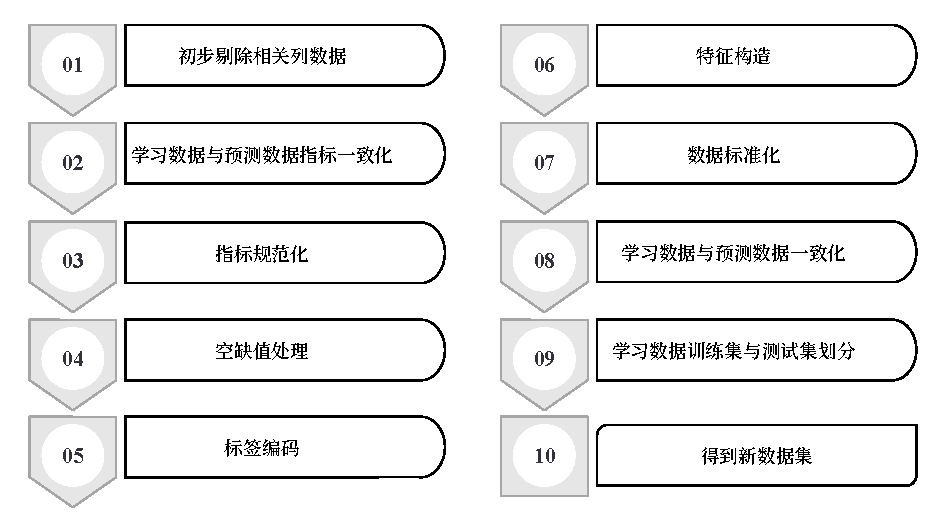
\includegraphics[scale=0.78]{数据的准备.pdf}}
		\caption{数据的准备主要过程}\label{fig:dataprepare}
	\end{figure}
	\subsection{数据的准备}
	为方便、准确、高效解决问题,我们需要对数据进行预处理,其主要过程见\textcolor{blue}{\cref{fig:dataprepare}},包括:初步剔除相关列数据、学习数据与预测数据指标一致化、指标规范化、空缺值处理、标签编码、特征构造、标准化、学习数据与预测数据一致化、学习数据训练集与测试集划分。\textbf{本文后续的模型建立都在此基础之上}。
	\subsubsection*{Step1 初步剔除相关列数据}
	由于“用户id”为连续编号,且与评分无任何关系,故本文将该列数据剔除;同时对于“用户描述”等文字性叙述指标,由于其均为文本,且描述特征难以提取,难以量化,本文将该列数据剔除,但为了获得客户相关描述,本文将绘制用户描述高频词汇云图;此外,对于“终端品牌类型”等多类别指标,由于其类别较多,量化后难以提取出有效信息,故也将其剔除,其余列暂时保留。
	\subsubsection*{Step2 学习数据与预测数据指标一致化}
	附件1与附件3为用户语音业务数据,但两表数据影响的因素存在不一致的现象,需要对指标取交集,确保两者一致,附件2与附件4同理。这里我们利用Python中集合set容器元素唯一性特征及pandas库,筛选出相同因素。而对于可能重合的指标,我们在下文也会进行一定处理。这样即可确保在学习数据上建立的模型依据的指标存在于预测数据集上,避免两者指标不一的情况。
	\subsubsection*{Step3 指标规范化}
	经过上述处理后,我们发现大部分影响因素为分类指标,其划分“是”“否”的字段不统一,故依据“附件5附件1、2、3、4的字段说明.xlsx”文件,本文对附件1、2、3、4中的分类指标进行规范化,记“是”类别为1,“否”类别为0,方便后续模型的建立。
	\subsubsection*{Step4 空缺值处理}
	在给定数据集中,部分空缺值可以依据附件5的解释进行填充。经过一定处理后,附件3与附件4中无空缺值,故本文对附件1与附件2中的空缺值进行分析与处理:
	\begin{itemize}
		\item \textbf{对于附件1}:据附件5解释进行填充后,还存在个别用户的空缺值,如\textcolor{blue}{\cref{fig:NaNView}}所示。
		\begin{figure}[h!t]
			\centerline{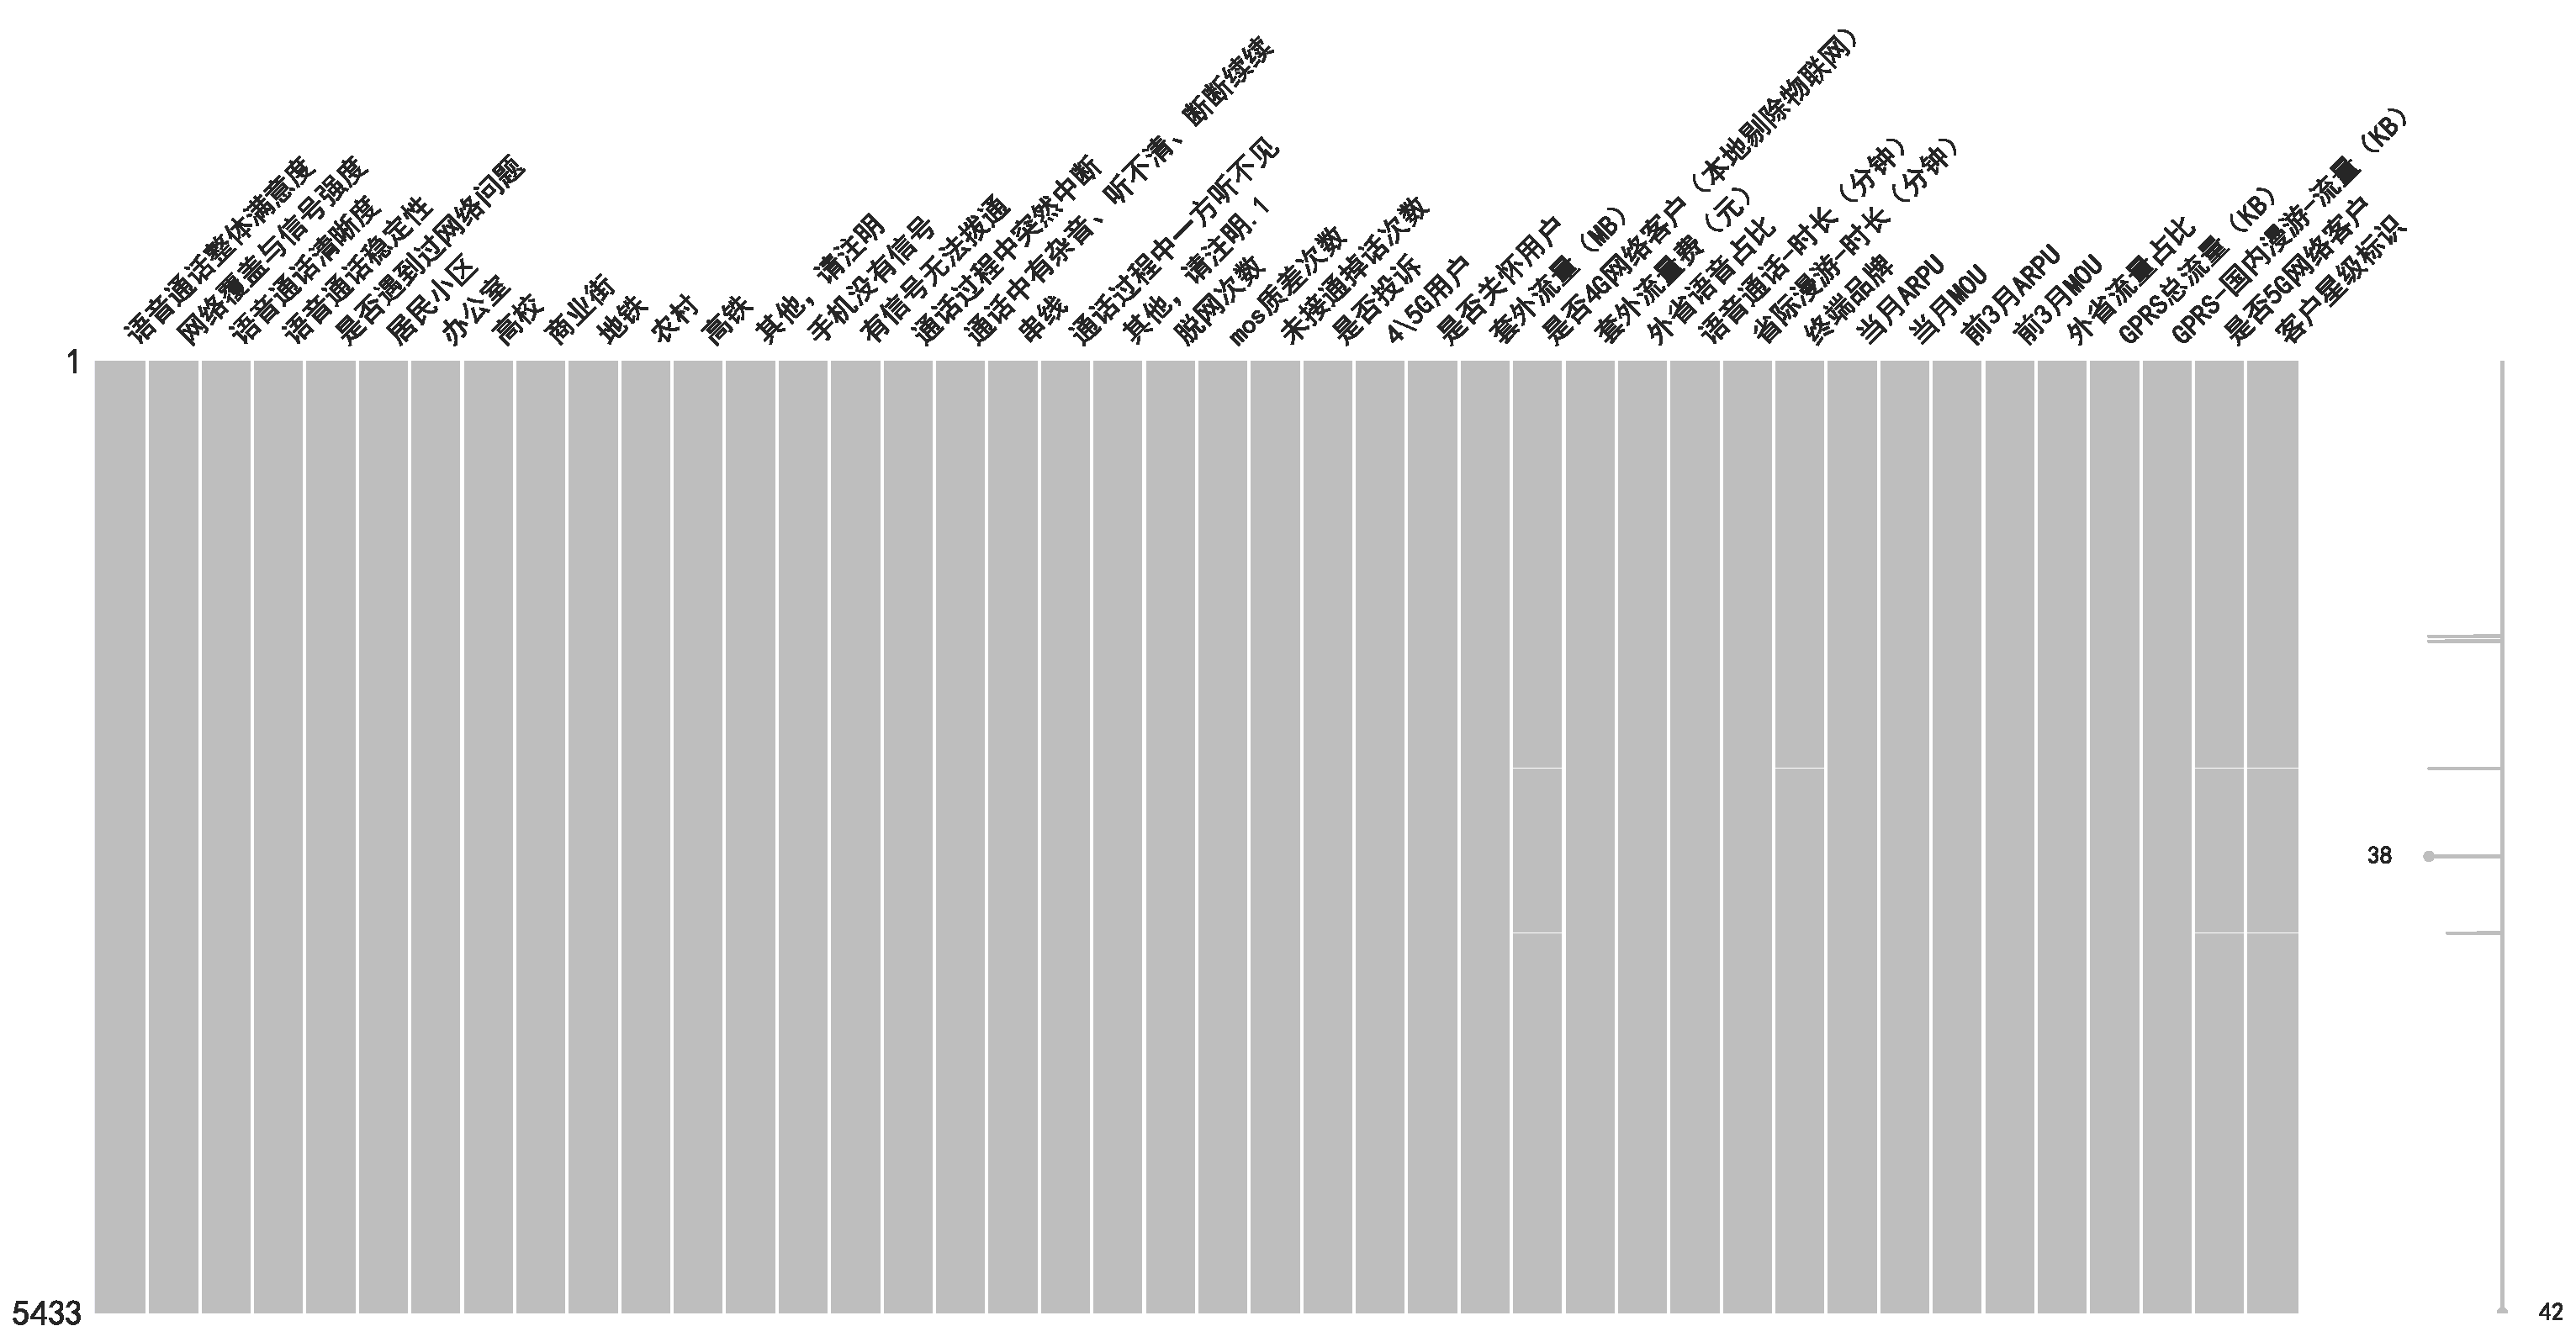
\includegraphics[scale=0.30]{[附件1]附件1空缺值可视化.pdf}}
			\caption{附件1初步处理后缺失值查看}\label{fig:NaNView}
		\end{figure}
		空缺值的列名为:“是否4G网络客户(本地剔除物联网)”“终端品牌”“是否5G网络客户”“客户星级标识”,且这些空缺值均在同一用户中出现,用户id分别为1573、1601、2326、2827、3265。附件1的空缺值有集中、个数少的特点,存有空缺值的用户仅有5个,占整体用户的$0.0920\%$,对于模型的建立影响较小,因此我们将这5行用户剔除。
		\item \textbf{对于附件2}:经过指标一致化后及初步数据空缺值的填补后,附件2中仅剩“终端品牌”列指标存在14个空缺值,根据该列数据其余特征,我们将这个14个空缺值以0填充。
	\end{itemize}
	\subsubsection*{Step5 标签编码}
	首先,对用户的评分进行编码,由于部分分类模型需要分类量值从0开始,因此,为方便后续集成学习等,本文将评分从$\left[1,10\right]$映射至$\left[0,9\right]$,且仍均为整数,即将评分减1。其次,对“终端品牌”“4\textbackslash{}5G用户”指标利用Python的sklearn库中的LabelEncoder进行标签编码。此外,对于“客户星级标识”指标,我们依据移动公司对客户星级标识的划分进行编码,编码值对应见\textcolor{blue}{\cref{tab:1}}。
	\begin{table}[htbp]
		\centering
		\caption{客户星级标识编码对应表}\label{tab:1}
		\scalebox{0.8}{
		\begin{tabular}{ccccccccc}
			\toprule
			未评级 & 准星 & 一星 & 二星 & 三星 & 银卡 & 金卡 & 白金卡 & 钻石卡 \\
			\midrule
			0 & 1 & 2 & 3 & 4 & 5 & 6 & 7 & 8 \\
			\bottomrule
		 \end{tabular}}
	\end{table}
	\subsubsection*{Step6 特征构造}
	观察并分析给定的数据,我们可以初步构造以下特征:
	\begin{itemize}
		\item \textbf{对于附件1与附件3}:观察到附件1中有“家宽投诉”与“资费投诉”两项,而在附件3中有“是否投诉”一项,因此,我们在附件1中构造“是否投诉”一项。若“家宽投诉”与“资费投诉”均为0,则“是否投诉”记为0,否则记为1。并同时删去“家宽投诉”与“资费投诉”。
		\item \textbf{对于附件2与附件4}:观察数据,我们构造三项新指标,分别为“出现问题场所或应用总”“网络卡速度慢延时大上不了网总”“质差总”。其来源为对应列指标按行求和。
	\end{itemize}
	\subsubsection*{Step7 数据标准化}
	该处标准化处理为\textbf{Z-score}方法,仅用于后续机器学习模型的使用。而在问题一的熵权法、灰色关联度分析中我们采用\textbf{Min-Max}方法,该方法在后文模型中会具体说明。

	对于某一列数据$x=\left[x_1,x_2,\cdots,x_m\right]^{\mathrm{T}}$,其平均值为
	\begin{equation}
		\mu=\frac{1}{m}\sum_{i=1}^{m}x_i \label{fmean}
	\end{equation}
	标准差为
	\begin{equation}
		\sigma=\sqrt{\frac{1}{m}\sum_{i=1}^{m}\left(x_i-\mu\right)^2} \label{fstd}
	\end{equation}
	则标准化后的数据为
	\begin{equation}
		\left(x_{\mathrm{standard}}\right)_i=\frac{x_i-\mu}{\sigma} \label{fstandardprocess}
	\end{equation}

	利用上述计算公式,我们对非分类指标进行处理,使得原数据经过处理后,其值聚集于0附近,即均值为0,标准差为1。这样处理,利于机器学习模型的建立、学习与预测,加快模型的收敛速度,并在一定程度上提升模型的准确性。同时该标准化处理方法适合当代嘈杂的大数据场景\textcolor{blue}{\cite{pstandard}}。因此对于大样本的数据,如出现部分异常值,使用该方法对最终结果影响较小。
	\subsubsection*{Step8 学习数据与预测数据一致化}
	经过上述几项处理后,我们还需要将附件1与附件3数据集一致化,包括指标一致化以及数据字段、分布排列一致化,从而保证对于需要预测的数据集附件3利用在附件1中建立的模型所利用到的数据集的一致性,避免造成数据的不一致,导致预测错误。本文对附件2与附件4进行上述相同的操作。
	\subsubsection*{Step9 学习数据训练集与测试集划分}
	为计算问题二中建立的模型的准确性等指标,需要在附件1与附件2中均划分训练集与测试集。对于语音业务划分训练集与测试集比例为8:2;而对于上网业务,其比例设为9:1。对于比例的设置,本文将在后文解释其合理性。且上述划分利用sklearn库中的train\_test\_split函数实现,且任意设定随机种子为2022,确保多次调试结果的一致性。该函数可确保划分的随机性,确保训练集与测试集数据分布规律大致相同。

	\subsection{问题一模型的建立与求解}
	对于问题一,我们综合\textbf{皮尔逊相关系数}、\textbf{熵权法}、\textbf{灰色关联度分析法},以及\textbf{随机森林分类模型},构建多元量化分析模型,尽可能准确挖掘到影响用户评分的因素。
	\subsubsection{模型的建立}
	\textbf{皮尔逊相关系数(Pearson Correlation Coefficient)}可衡量两个变量之间的相似度,我们不妨用$\rho\left(x,y\right)$表示,计算公式\textcolor{blue}{\cite{ppearson1}}如下
	\begin{equation}
	\rho\left(x,y\right)=\frac{\sum\limits_{i=1}^{n}\left(x_{i}-\mu_x\right)\left(y_{i}-\mu_y\right)}{\sqrt{\sum\limits_{i=1}^{n}\left(x_{i}-\mu_x\right)^{2}}\sqrt{\sum\limits_{i=1}^{n}\left(y_{i}-\mu_y\right)^{2}}} \label{fpearson}
	\end{equation}
	其中$\mu$计算见\textcolor{blue}{\eqref{fmean}}。

	由该定义,显然$\rho\in[-1,1]$。当$\rho>0$时,上述两变量呈正相关;当$\rho=0$时,上述两变量不相关;当$\rho<0$时,上述两变量呈负相关。当$\left|\rho\right|$越接近于$1$时,则上述两变量相关性就越强\textcolor{blue}{\cite{ppearson2}}。
\newpage
	\textbf{熵权法(Entropy Weight Method, EWM)}是一种指标客观影响程度的量化方法。当信息熵越大时,信息的无序程度越大,此时,信息价值越小,指标权重就越小\textcolor{blue}{\cite{pewm1}}。其计算步骤如下:
	\begin{itemize}
		\item \textbf{Step1},指标正向化。由于数据集构成的指标类别不一,部分指标可能数值越大越好,部分指标可能越小越好,而有的可能在某一点取值最优,为方便、高效评价,我们需要进行指标正向化处理\textcolor{blue}{\cite{pewm2}}。其处理方法如下
		\begin{itemize}
			\item {\heiti 越大越优指标}
			\begin{equation}
				x'_{ij}=x_{ij} \label{fmax}
			\end{equation}
			\item {\heiti 越小越优指标}
			\begin{equation}
				x'_{ij}=\mathrm{max}\left(x_{ij}\right)-x_{ij} \label{fmin}
			\end{equation}
			\item {\heiti 在$\beta$处取值最优指标}
			\begin{equation}
				x'_{ij}=1-\frac{\left|x_{ij}-\beta\right|}{\mathrm{max}\left(\left|x_{ij}-\beta\right|\right)} \label{fmid}
			\end{equation}
		\end{itemize}
		\item \textbf{Step2},数据标准化。由于数据集构成的指标数据数量级存在差异、量纲不一,为消除上述情况对结果的影响,我们需要将各指标进行标准化处理,这里我们使用Min-Max方法。处理方法计算公式如下
		\begin{equation}
			r_{ij}=\frac{x'_{ij}-\mathrm{min}\left(x'_{j}\right)}{\mathrm{max}\left(x'_{j}\right)-\mathrm{min}\left(x'_{j}\right)} \label{Min-Max}
		\end{equation}
		\item \textbf{Step3},计算信息熵。进行上述处理后可得到由特征数据构成的矩阵$R\left(r_{ij}\right)_{m\times n}$,对于某一项指标的数据$r_j$,其信息熵为
		\begin{equation}
			E_j=-\frac{1}{\ln m}\cdot\sum\limits_{i=1}^{m}p_{ij}\ln p_{ij} \label{fentropyj}
		\end{equation}
		其中
		\begin{equation}
			p_{ij}=\frac{r_{ij}}{\sum\limits_{i=1}^{m}r_{ij}} \label{fpij}
		\end{equation}
		观察到\textcolor{blue}{\eqref{fpij}}中分母不可为$0$,且\textcolor{blue}{\eqref{fentropyj}}对数真数部分不能为$0$,因此,我们在进行\textbf{Step2}时,标准化区间的最小值设为$0.002$,可避免计算时的不合定义。
		\item \textbf{Step4},计算指标权重。其计算公式如下
		\begin{equation}
			\omega_j=\frac{1-E_j}{\sum\limits_{j=1}^{n}\left(1-E_j\right)} \label{fwj}
		\end{equation}
	\end{itemize}
\newpage
	\textbf{灰色关联度分析(Grey Relation Analysis, GRA)}是通过指标之间的关联系数来判断指标对系统的影响程度\textcolor{blue}{\cite{pgrey1}}。其计算方法如下:
	\begin{itemize}
		\item \textbf{Step1},指标无量纲化。这里指标无量纲化与熵权法的\textbf{Step2}中的数据标准化方法处理相同,此处不再赘述。
		\item \textbf{Step2},计算每一项比较序列与参考序列绝对值差
		\begin{equation}
			\Delta i\left(k\right)=\left|R_0\left(k\right)-R_i\left(k\right)\right| \label{fDeltaik}
		\end{equation}
		\item \textbf{Step3},确定二级最小差与二级最大差
		\begin{equation}
			\underset{i=1}{\overset{n}{\max}}\underset{k=1}{\overset{m}{\max}}\left| R_0\left( k \right) -R_i\left( k \right) \right| \qquad \underset{i=1}{\overset{n}{\min}}\underset{k=1}{\overset{m}{\min}}\left| R_0\left( k \right) -R_i\left( k \right) \right| \label{fmaxmaxminmin}
		\end{equation}

		\item \textbf{Step4},计算关联系数,记分辨系数为$\eta$,本文我们取$\eta=0.5$
		\begin{equation}
			\xi_i\left(k\right)=\frac{\underset{i}{\min}\underset{k}{\min}\left| R_0\left( k \right) -R_i\left( k \right) \right|+\eta \cdot \underset{i}{\max}\underset{k}{\max}\left| R_0\left( k \right) -R_i\left( k \right) \right|}{\left| R_0\left( k \right) -R_i\left( k \right) \right|+\eta \cdot \underset{i}{\max}\underset{k}{\max}\left| R_0\left( k \right) -R_i\left( k \right) \right|} \label{fxi}
		\end{equation}
		\item \textbf{Step5},计算灰色关联度
		\begin{equation}
			\gamma_{0i}=\frac{1}{m}\sum\limits_{k=1}^{m}\xi_i\left(k\right) \label{fgamma}
		\end{equation}
	\end{itemize}

	\textbf{随机森林(Random Forest, RF)}是由多棵决策树(Decision Tree)进行组合后对预测结果投票或取均值的一种算法\textcolor{blue}{\cite{prf}}。其有分类和回归两种模型,对于本题,我们选择分类模型。其简要过程如\textcolor{blue}{\cref{fig:RF}}所示,算法伪代码如\textcolor{blue}{Algorithm\ref{RFfunction}}所示。
	
	\scalebox{0.88}{
	\begin{algorithm}[H]
		\label{RFfunction}
		\KwData{数据集$\mathcal{D}$}
		\textbf{function} DTree$\left(\mathcal{D}\right)$\
		
		\eIf{Termination}
		{\textbf{return} $\mathrm{base}\left(g_t\right)$}
		{\textbf{learn} $b\left(x\right)$并且依据$b\left(x\right)$划分$\mathcal{D}$为$\mathcal{D}_C$\

		\textbf{build} $G_C \leftarrow$ DTree($\mathcal{D}_C$)\

		\textbf{return} $G\left(x\right)=\sum\limits_{C=1}^{C}[\![b\left(x\right)=C]\!]G_C\left(x\right)$}
		
		\textbf{function} RandomForest$\left(\mathcal{D}\right)$\
		
		\For{$t=1,2,3,\cdots,T$}{\textbf{request} 数据集$\tilde{\mathcal{D}}_t \leftarrow$ BoostStrapping$\left(\mathcal{D}\right)$\
		
		\textbf{obtain} DTree $g_t\leftarrow$ DTree$\left(\tilde{\mathcal{D}}_t\right)$\

		\textbf{return} $G=$ Uniform$\left(g_t\right)$
		}
		
		\KwResult{随机森林模型$G=\mathrm{Uniform}\left(g_t\right)$}
		\caption{随机森林(RF)}
	\end{algorithm}}
	\begin{figure}[H]
		\centerline{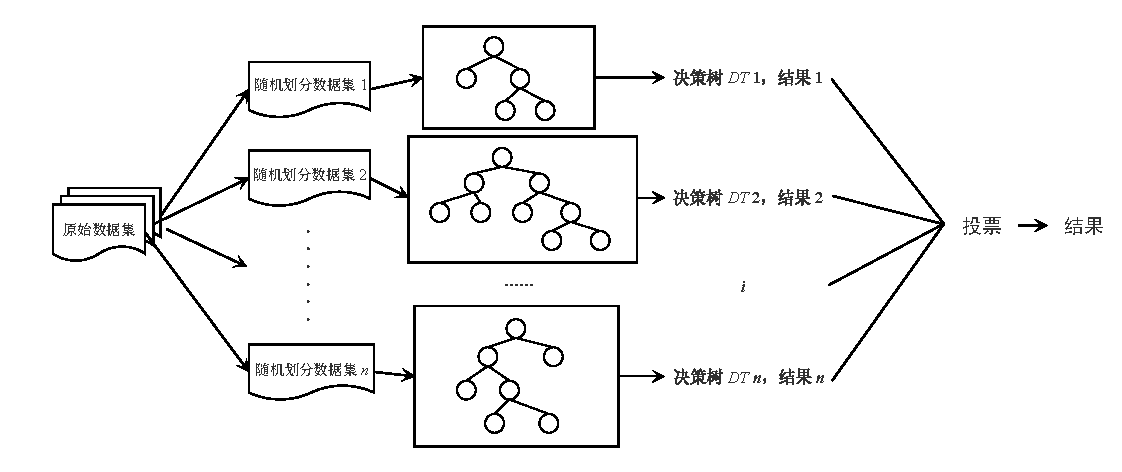
\includegraphics[scale=0.80]{随机森林简图.pdf}}
		\caption{随机森林算法简图}\label{fig:RF}
	\end{figure}
	
	对于单棵决策树而言,本文利用\textbf{CART}算法\textcolor{blue}{\cite{prf}}构建。基尼系数是衡量样本集合纯度的指标,当该值越小时,其纯度也就越高。计算公式如下
	\begin{equation}
		Gini\left( R_i \right)=\sum\limits_{k=1}^{K}\sum\limits_{k\ne k'}P_k P_{k'}=1-\sum\limits_{k=1}^{K}P_k^2 \label{fGini}
	\end{equation}
	其中,$R$为选取出的特征(影响因素),$K$表示在该特征中包含的类别数,$P_k$表示该特征中第$k$类别的出现概率。

	由上述分析可知,对于单棵决策树而言,其叶子节点的分裂特征为选择的所有特征中基尼系数最小的特征。

	\subsubsection{语音业务求解}
	首先我们绘制语音业务用户四项评分箱线图,如\textcolor{blue}{\cref{fig:a1box4mark}}所示(图中数据是原评分数据通过标签编码转化而来的)。之后依据\textcolor{blue}{\eqref{fpearson}},可以计算出各影响因素与语音业务四项评分之间的皮尔逊相关系数,并通过Python绘制其热力图,如\textcolor{blue}{\cref{fig:a1pearson}}所示,图中仅显示相关性排名前10的指标。
	\begin{figure}[htbp]
		\centering
		\begin{minipage}{0.48\linewidth}
			\centering
			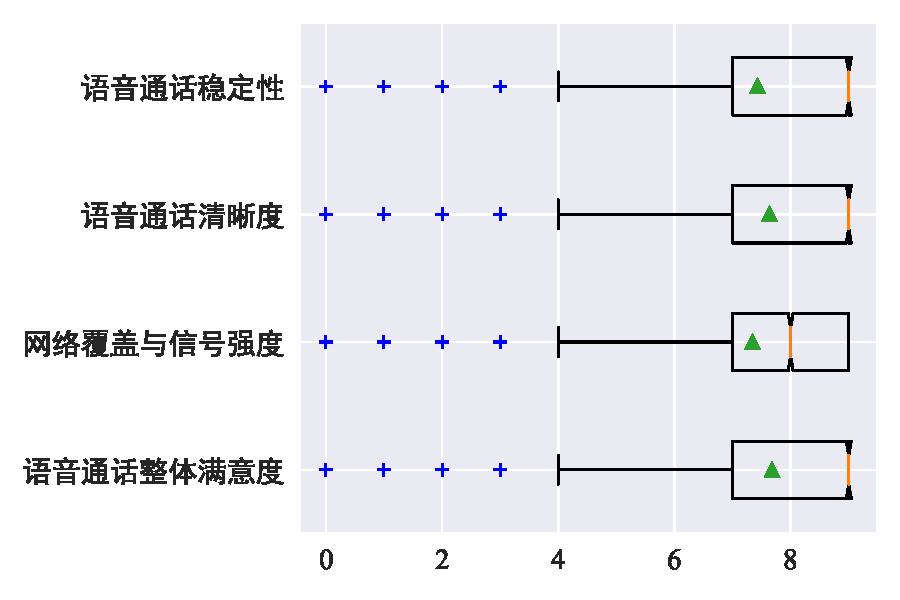
\includegraphics[width=1.0\linewidth]{[附件1][语音通话整体满意度、网络覆盖与信号强度、语音通话清晰度、语音通话稳定性]评分箱线图.pdf}
			\caption{语音业务用户四项评分箱线图}
			\label{fig:a1box4mark}
		\end{minipage}
		%\qquad
		\begin{minipage}{0.48\linewidth}
			\centering
			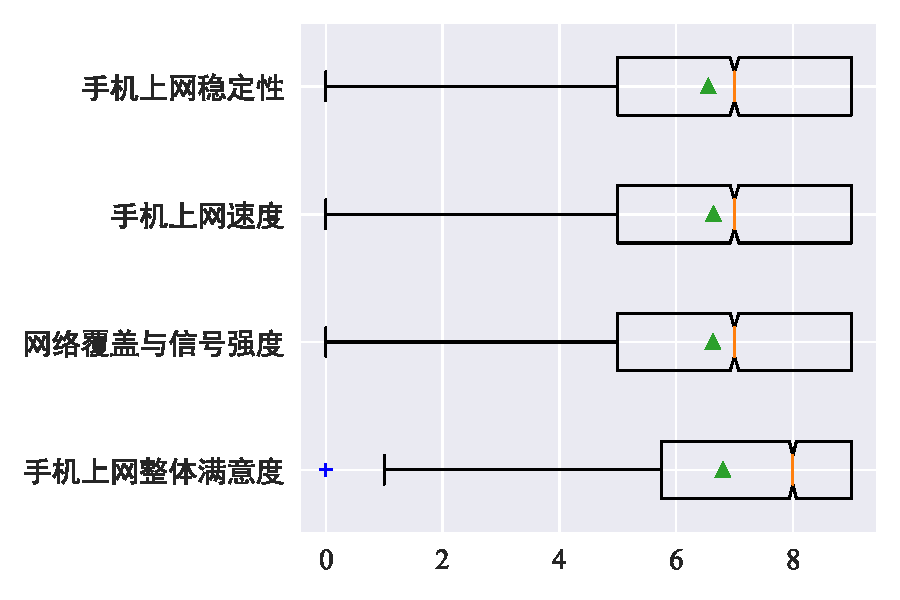
\includegraphics[width=1.0\linewidth]{[附件2][手机上网整体满意度、网络覆盖与信号强度、手机上网速度、手机上网稳定性]评分箱线图.pdf}
			\caption{上网业务用户四项评分箱线图}
			\label{fig:a2box4mark}
		\end{minipage}
	\end{figure}
	\begin{figure}[h!t]
		\centerline{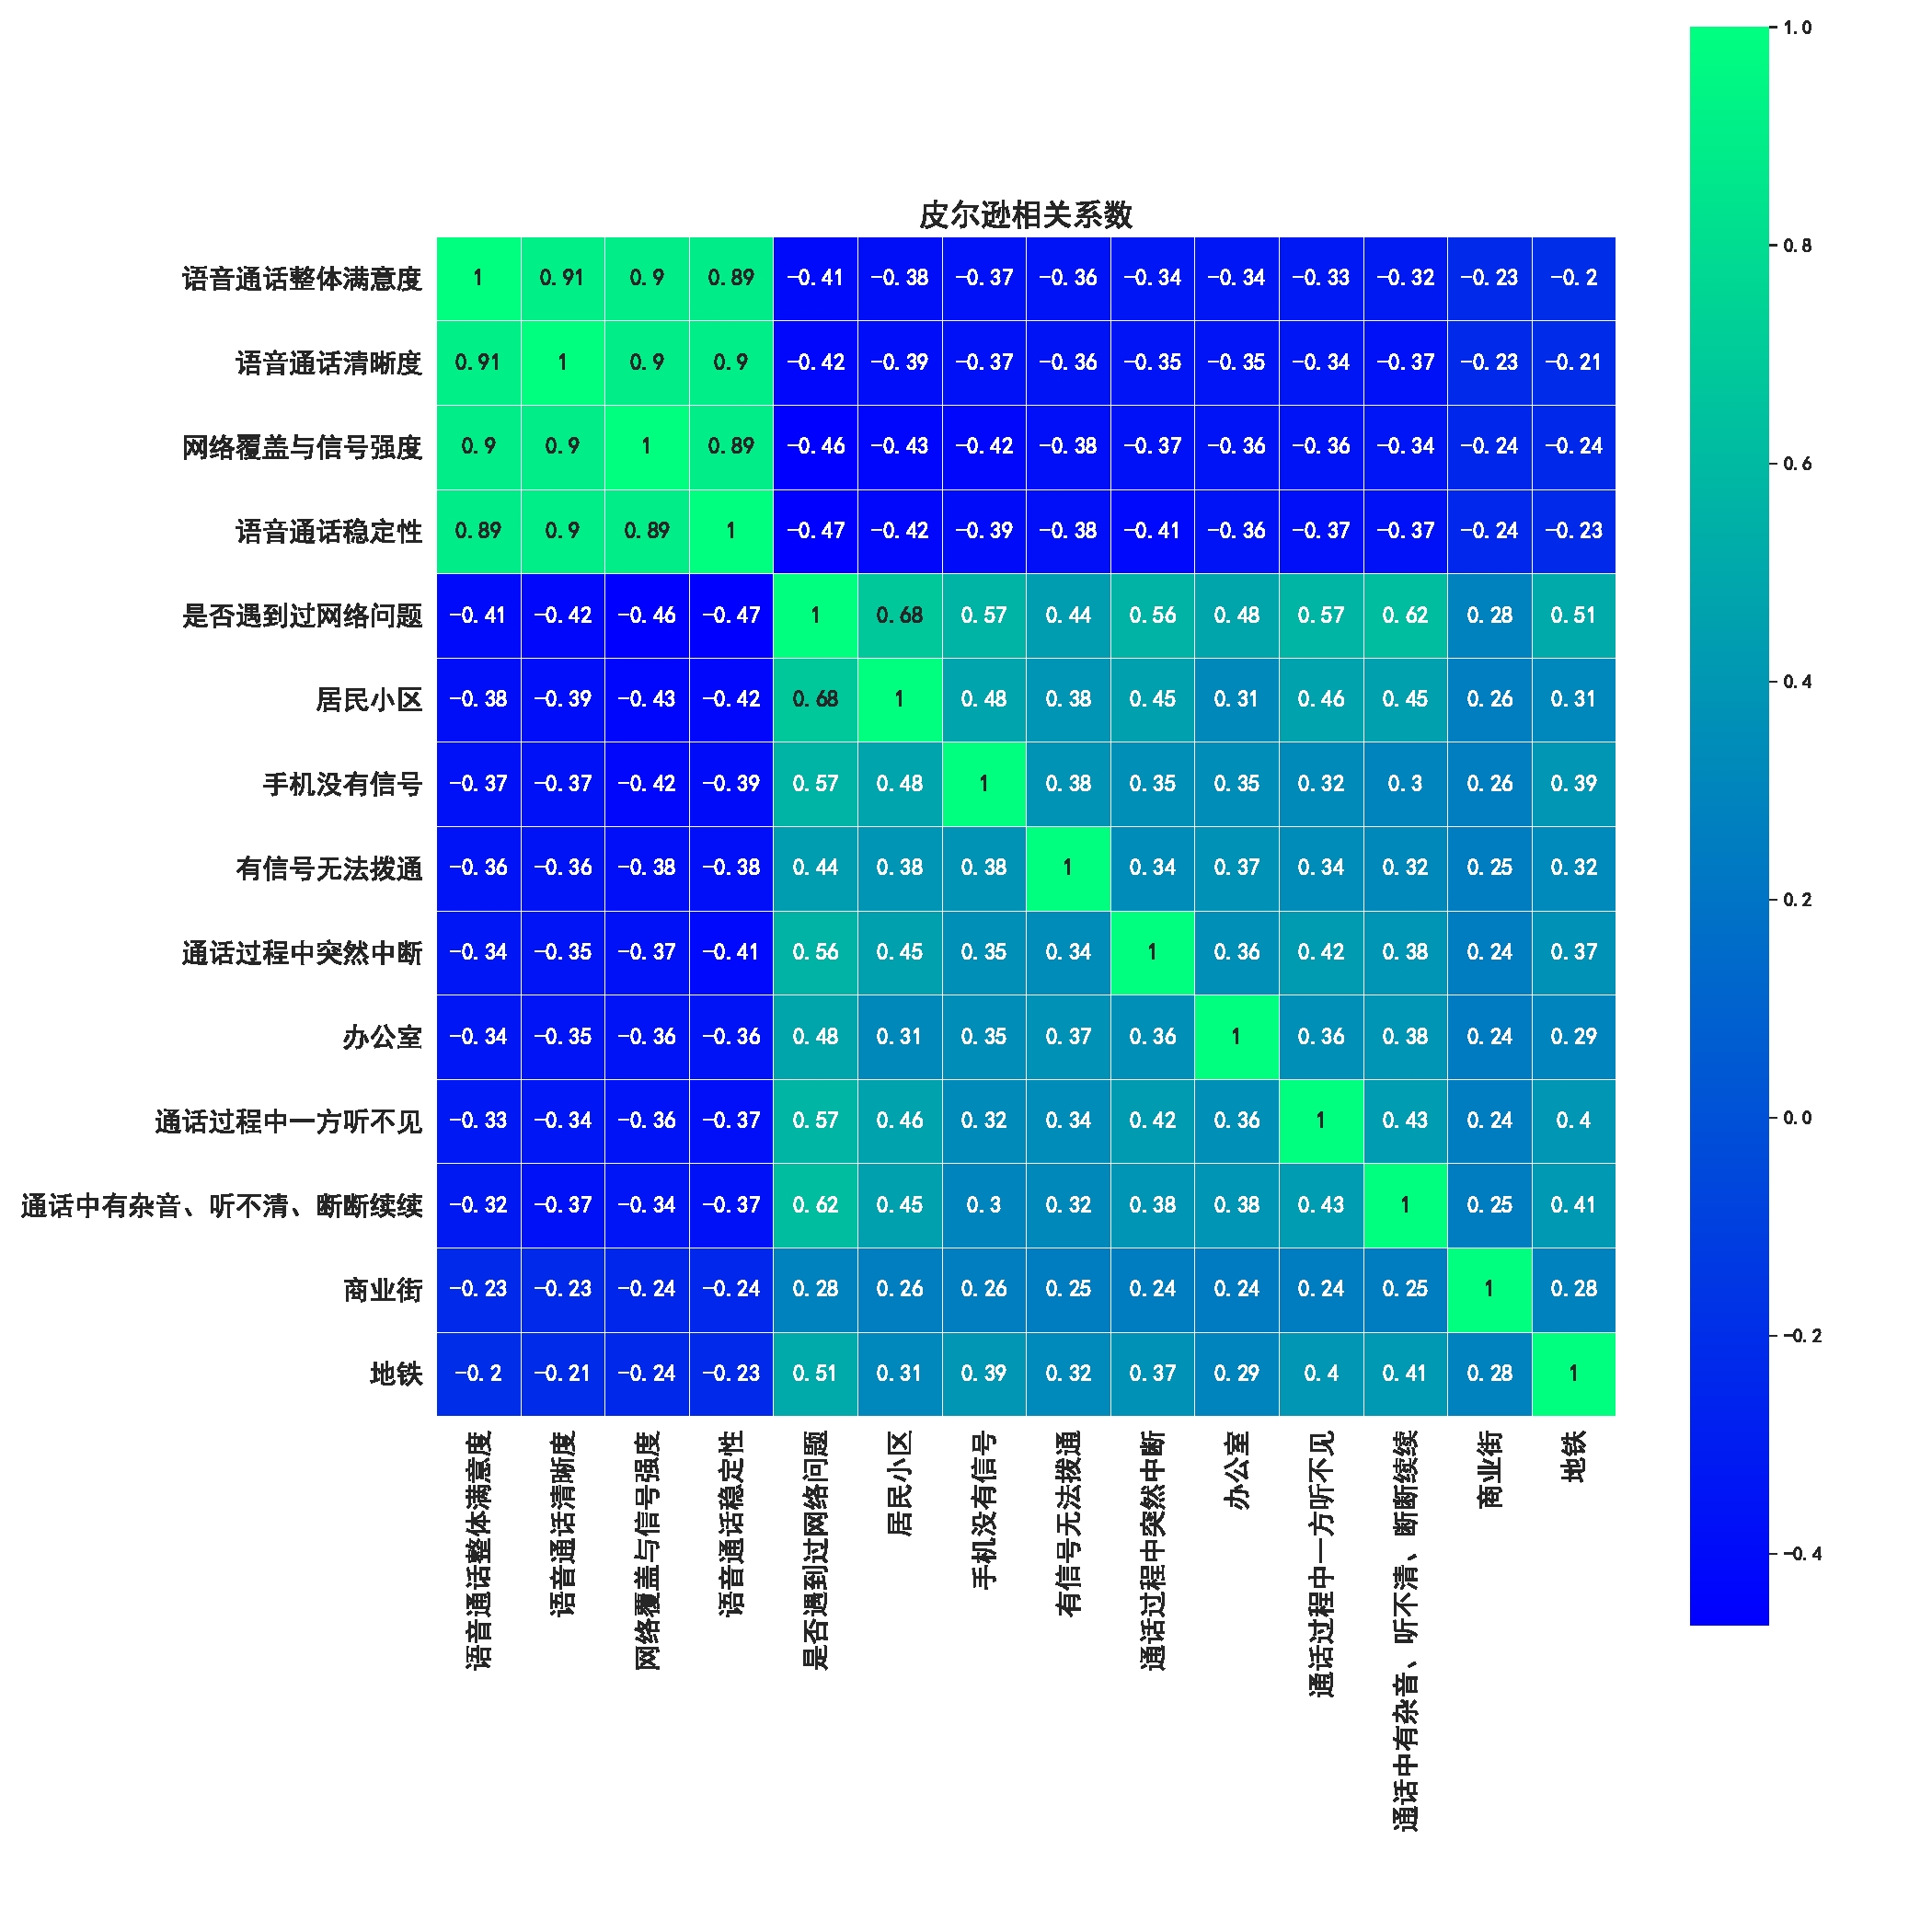
\includegraphics[scale=0.4]{[附件1]皮尔逊相关系数(14个).pdf}}
		\caption{语音业务评分与其影响因素皮尔逊相关系数热力图}\label{fig:a1pearson}
	\end{figure}
	由\textcolor{blue}{\cref{fig:a1pearson}}可以直观发现,用户对于语音业务的满意度影响较大排名在前的因素依次为“是否遇到过网络问题”、“居民小区”、“手机没有信号”、“有信号无法拨通”、“通话过程中突然中断”、“办公室”、“通话过程中一方听不见”、“通话中有杂音、听不清、断断续续”、“商业街”、“地铁”。为了更好地分析影响语音业务的因素,我们分别绘制出上述10个指标与语音业务四项评分之间的RidViz图,如\textcolor{blue}{\cref{fig:a1FirstRid}}\textasciitilde\textcolor{blue}{\cref{fig:a1FourthRid}}所示。由此我们可以发现,用户对于语音业务的四项评分,分布规律大致一致,且主要影响满意度的因素非常相似,同时噪声较小。因此我们在此分析基础上,建立熵权法、灰色关联度分析法、随机森林模型在整体上求得量化结果并得出主要因素。结果见\textcolor{blue}{\cref{tab:a1ewm}}、\textcolor{blue}{\cref{tab:a1grey}}、\textcolor{blue}{\cref{fig:a1allRF}},其中\textcolor{blue}{\cref{fig:a1allRF}}中数据见\textcolor{blue}{\cref{tab:a1allquantization}}最后一列。
	
	通过分析上述图表,我们可以发现利用熵权法、灰色关联度分析法、随机森林模型得到的排序结果大致相同,主要影响因素有:“省际漫游-时长(分钟)”、“前3月ARPU”、“套外流量(MB)”、“GPRS-总流量(KB)”、“套外流量费(元)”、“脱网次数”、“未接通掉话次数”、“mos质差次数”、“其他,请注明.1”(该指标对应的是通话过程中遇到其他问题部分的注明)、“是否投诉”(特征构造出的因素)、“是否关怀用户”、“串线”、“其他,请注明”(该指标对应的是出现问题的场所部分的注明),以及在各场所遇到语音通话各个问题的情况。而在随机森林模型中,我们可以发现有部分因素量化值也排名较前,如“当月ARPU”、“是否遇到过网络问题”、“前3月MOU”、“语音通话-时长(分钟)”、“当月MOU”、“客户星级标识”、“终端品牌”等因素。可以发现,随机森林模型可以给出更多的重要影响因素,避免了熵权法及灰色关联度分析的局限性,并且量化值可以用于后续模型的建立。

	因此我们在此分析基础上,将语音业务的四项评分分别作为因变量,所有指标作为自变量(不包括评分),建立随机森林模型,绘制出其特征重要性图示,由于篇幅原因,读者可翻阅附录,见\textcolor{blue}{\cref{fig:a1FirstRF}}\textasciitilde\textcolor{blue}{\cref{fig:a1FourthRF}}。以及量化各影响因素影响程度,量化结果见\textcolor{blue}{\cref{tab:a1allquantization}}。
	\begin{figure}[htbp]
		\centering
		\begin{minipage}{0.49\linewidth}
			\centering
			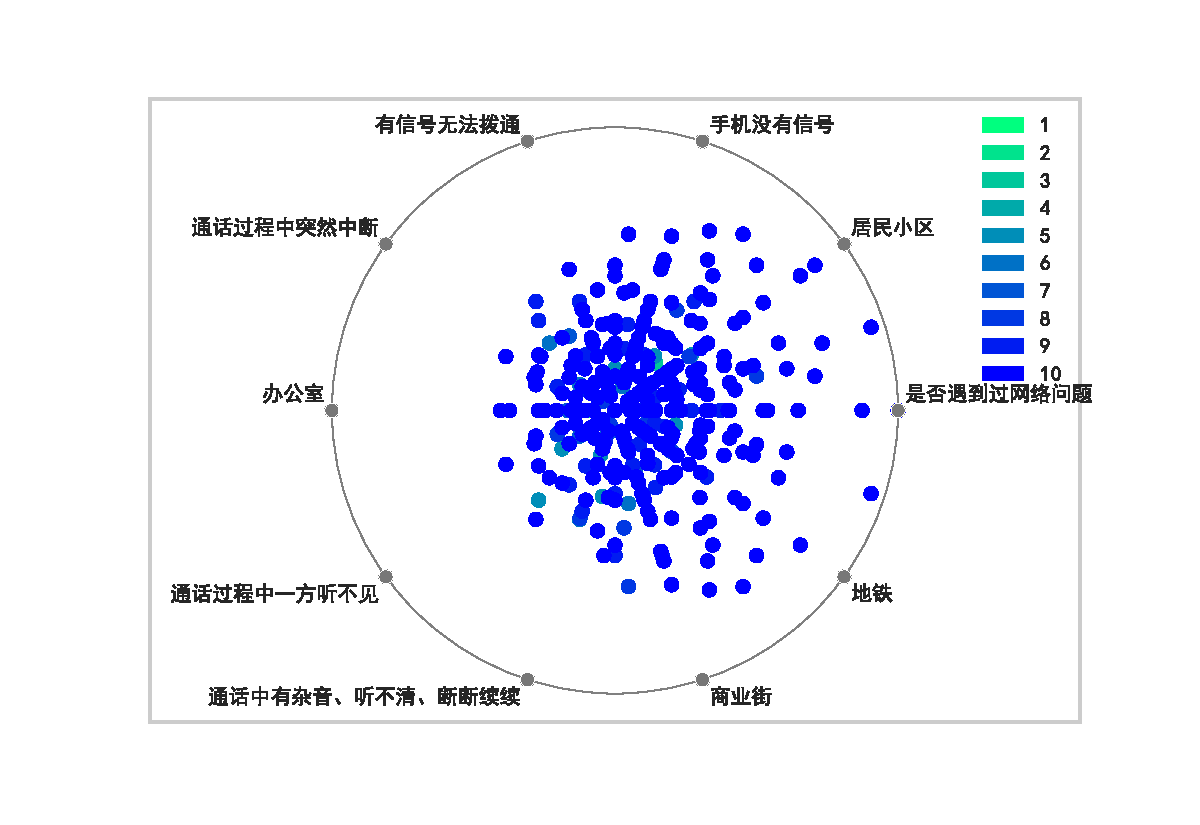
\includegraphics[width=0.9\linewidth]{[附件1]语音通话整体满意度RidViz.pdf}
			\caption{语音通话整体满意度与指标RidViz}
			\label{fig:a1FirstRid}
		\end{minipage}
		\begin{minipage}{0.49\linewidth}
			\centering
			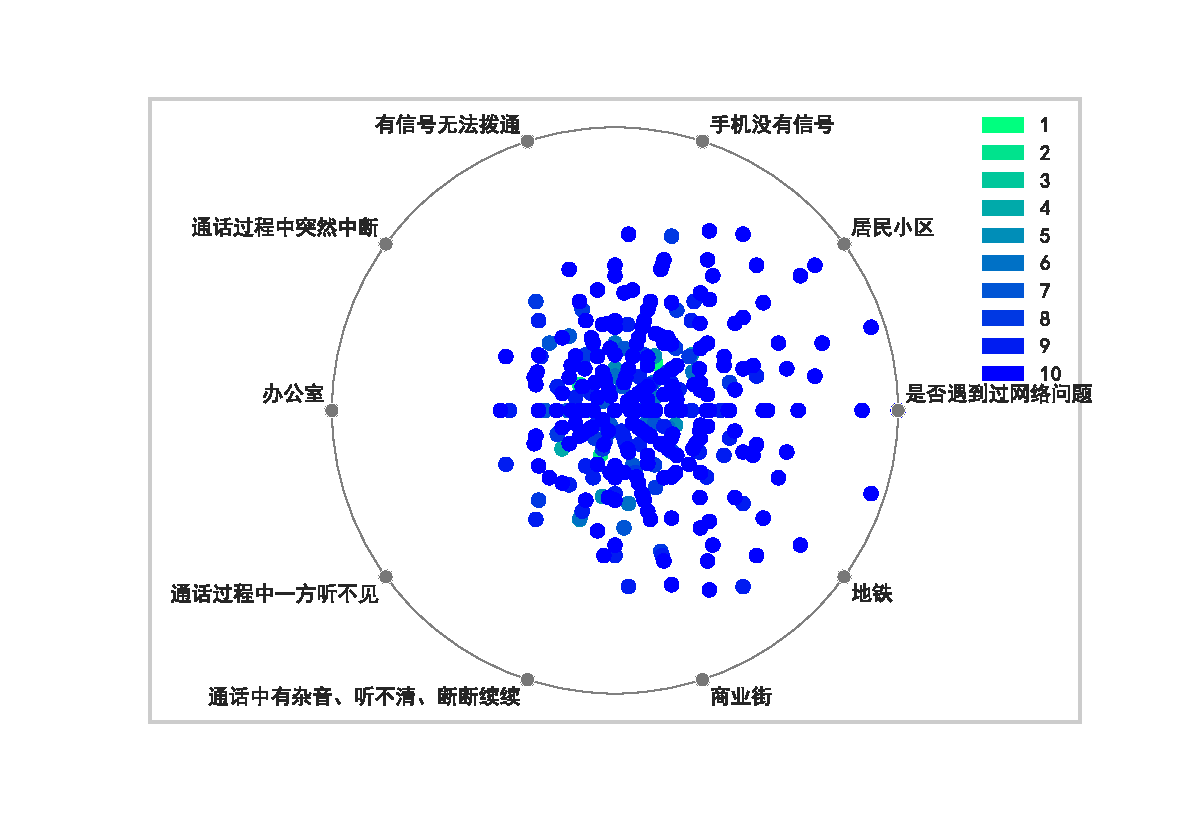
\includegraphics[width=0.9\linewidth]{[附件1]网络覆盖与信号强度RidViz.pdf}
			\caption{网络覆盖与信号强度与指标RidViz}
			\label{fig:a1SecondRid}
		\end{minipage}
		
		\begin{minipage}{0.49\linewidth}
			\centering
			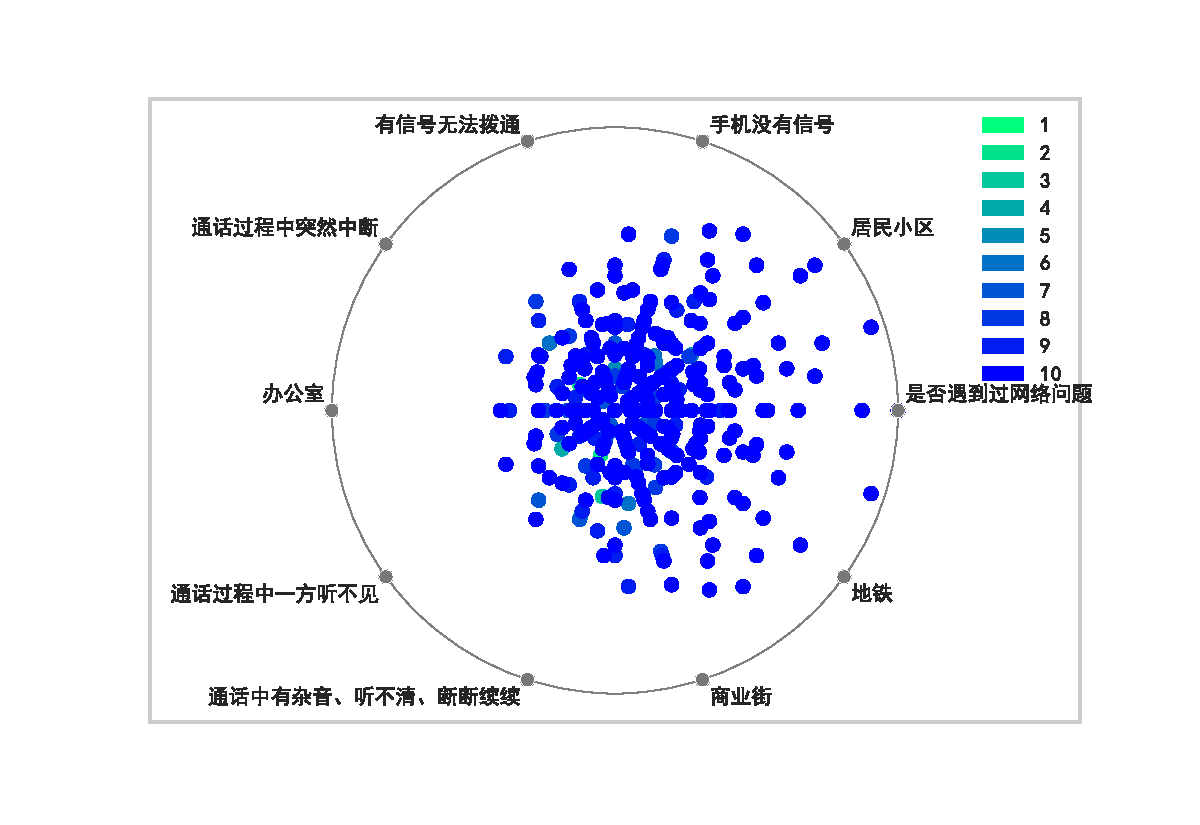
\includegraphics[width=0.9\linewidth]{[附件1]语音通话清晰度RidViz.pdf}
			\caption{语音通话清晰度与指标RidViz}
			\label{fig:a1ThirdRid}
		\end{minipage}
		\begin{minipage}{0.49\linewidth}
			\centering
			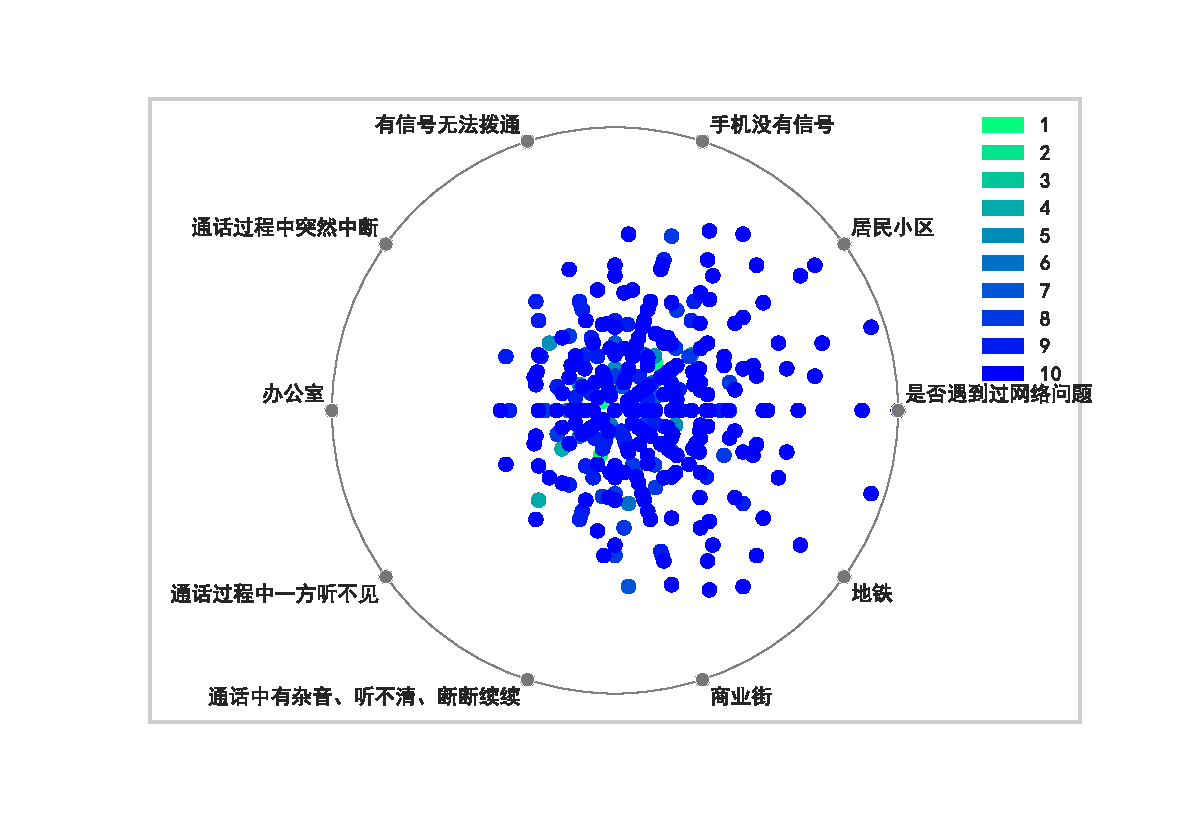
\includegraphics[width=0.9\linewidth]{[附件1]语音通话稳定性RidViz.pdf}
			\caption{语音通话稳定性RidViz}
			\label{fig:a1FourthRid}
		\end{minipage}
	\end{figure}

	\begin{figure}[h!t]
		\centerline{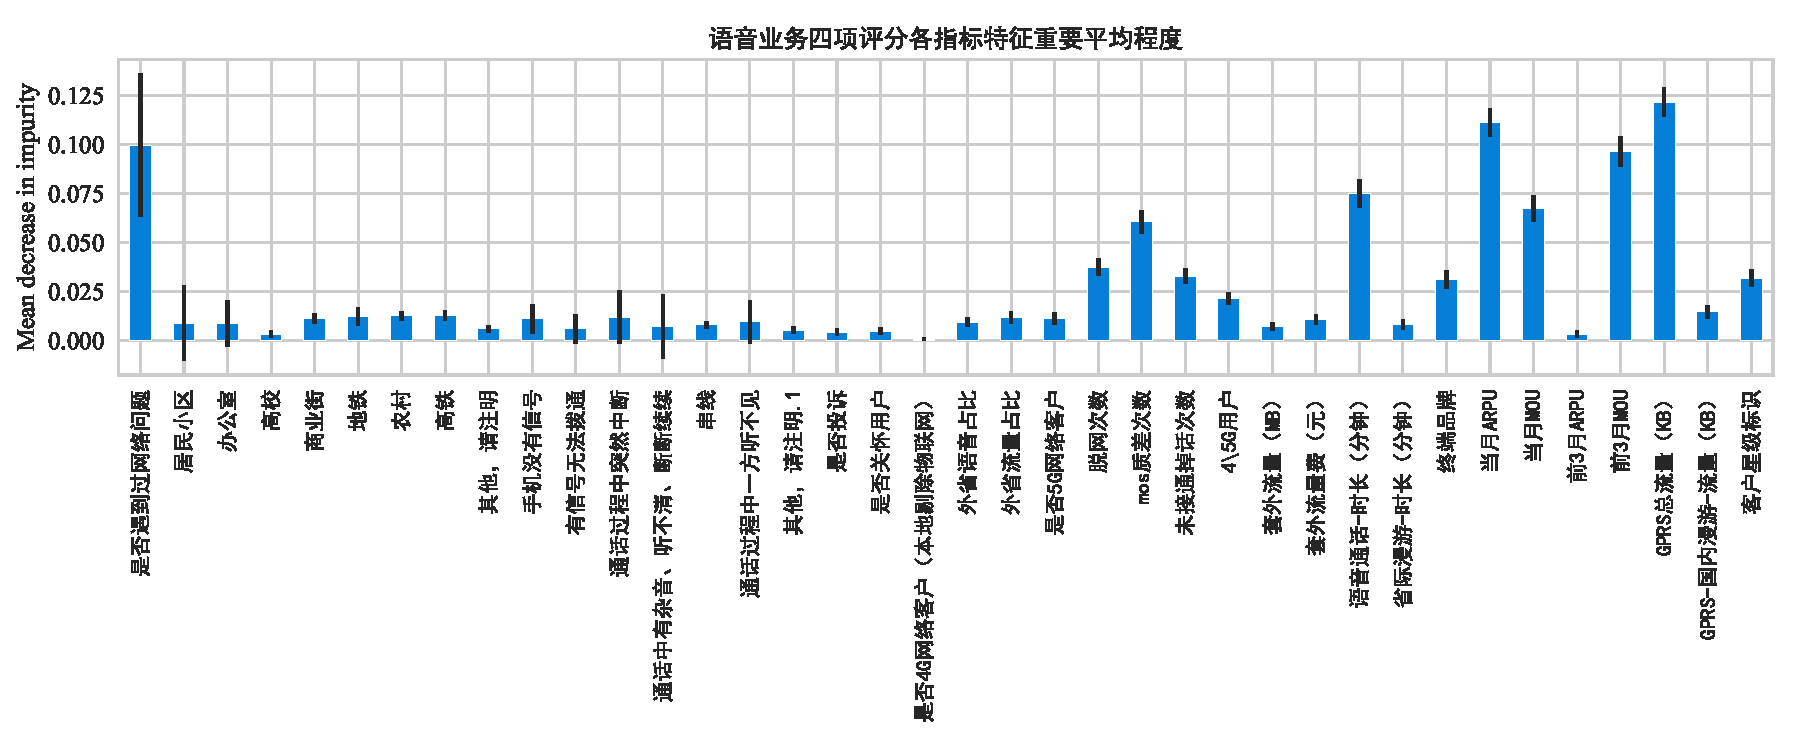
\includegraphics[scale=0.40]{[附件1]语音业务四项评分各指标特征重要平均程度.pdf}}
		\caption{语音业务四项评分各指标特征重要平均程度}\label{fig:a1allRF}
	\end{figure}

	通过分析\textcolor{blue}{\cref{fig:a1FirstRF}}\textasciitilde\textcolor{blue}{\cref{fig:a1FourthRF}}以及\textcolor{blue}{\cref{tab:a1allquantization}},我们可以得到以下结论:
	\begin{itemize}
		\item 对于\textbf{语音通话整体满意度},影响客户满意度的主要因素有:“当月ARPU”、“GPRS总流量(KB)”、“语音通话-时长(分钟)”、“mos质差次数”、“手机没有信号”、“未接通掉话次数”、“有信号无法拨通”、“通话中有杂音、听不清、断断续续”、“通话过程中突然中断”、“通话过程中一方听不见”,以及在各场所发生上述情况;
		\item 对于\textbf{网络覆盖与信号强度},影响客户满意度的主要因素有:“GPRS总流量(KB)”、“前3月MOU”、“当月ARPU”、“是否遇到过网络问题”、“mos质差次数”、“脱网次数”、“语音通话-时长(分钟)”、“手机没有信号”,以及在各场所发生上述情况;
		\item 对于\textbf{语音通话清晰度},影响客户满意度的主要因素有:“GPRS总流量(KB)”、“前3月MOU”、“当月ARPU”、“通话中有杂音、听不清、断断续续”、“mos质差次数”、“语音通话-时长(分钟)”、“未接通掉话次数”,以及在各场所发生上述情况;
		\item 对于\textbf{语音通话稳定性},影响客户满意度的主要因素有:“GPRS总流量(KB)”、“当月ARPU”、“语音通话-时长(分钟)”、“前3月MOU”、“mos质差次数”、“终端品牌”、“未接通掉话次数”、“客户星级标识”、“脱网次数”、“通话过程中突然中断”、“通话过程中一方听不见”、“手机没有信号”、“通话中有杂音、听不清、断断续续”、“有信号无法拨通”,以及在各场所发生上述情况;
		\item 对于\textbf{语音业务四项评分},我们可以发现,影响客户满意度的主要因素大致相同,在不同的评分中,其量化出的影响程度不相同,但大致趋势一致。
	\end{itemize}

	通过上述模型的建立,我们得到了符合预期的效果。本文进行综合比较,可以更全面地分析出影响的主要因素,而对于量化值,我们以随机森林结果为准,这是由于该量化值更贴近于生活、可以更好地挖掘出其中隐含的因素,同时在后续模型的建立中,本文也会利用该结果进行分析,对于影响语音业务用户评分的因素量化最终结果见\textcolor{blue}{\cref{tab:a1allquantization}}。
	\begin{table}[htbp]
	\centering
	\caption{语音业务总体以及四项评分各个指标影响程度量化结果}
	\setlength{\aboverulesep}{0pt}
	\setlength{\belowrulesep}{0pt}
	\scalebox{0.62}{
	  \begin{tabular}{c|cccc|c}
	  \toprule
	  \textbf{因素} & \textbf{语音通话整体满意度} & \textbf{网络覆盖与信号强度} & \textbf{语音通话清晰度} & \textbf{语音通话稳定性} & \textbf{语音业务总} \\
	  \midrule
	  GPRS总流量(KB) & 0.1266  & 0.1151  & 0.1181  & 0.1263  & 0.1215  \\
	  当月ARPU & 0.1154  & 0.1116  & 0.1000  & 0.1032  & 0.1111  \\
	  是否遇到过网络问题 & 0.0922  & 0.1015  & 0.0953  & 0.1080  & 0.0995  \\
	  前3月MOU & 0.0996  & 0.1232  & 0.1028  & 0.0993  & 0.0964  \\
	  语音通话-时长(分钟) & 0.0726  & 0.0762  & 0.0754  & 0.0680  & 0.0747  \\
	  当月MOU & 0.0671  & 0.0715  & 0.0722  & 0.0689  & 0.0673  \\
	  mos质差次数 & 0.0645  & 0.0512  & 0.0617  & 0.0670  & 0.0604  \\
	  脱网次数  & 0.0388  & 0.0406  & 0.0361  & 0.0444  & 0.0372  \\
	  未接通掉话次数 & 0.0334  & 0.0319  & 0.0328  & 0.0302  & 0.0327  \\
	  客户星级标识 & 0.0315  & 0.0233  & 0.0259  & 0.0243  & 0.0316  \\
	  终端品牌  & 0.0356  & 0.0297  & 0.0368  & 0.0382  & 0.0310  \\
	  4\textbackslash{}5G用户 & 0.0114  & 0.0137  & 0.0177  & 0.0119  & 0.0212  \\
	  GPRS-国内漫游-流量(KB) & 0.0105  & 0.0112  & 0.0162  & 0.0136  & 0.0145  \\
	  高铁    & 0.0107  & 0.0114  & 0.0141  & 0.0118  & 0.0124  \\
	  农村    & 0.0117  & 0.0106  & 0.0105  & 0.0076  & 0.0124  \\
	  地铁    & 0.0151  & 0.0126  & 0.0152  & 0.0129  & 0.0121  \\
	  通话过程中突然中断 & 0.0081  & 0.0134  & 0.0096  & 0.0075  & 0.0117  \\
	  外省流量占比 & 0.0133  & 0.0125  & 0.0110  & 0.0094  & 0.0115  \\
	  是否5G网络客户 & 0.0116  & 0.0090  & 0.0128  & 0.0091  & 0.0112  \\
	  商业街   & 0.0096  & 0.0080  & 0.0124  & 0.0071  & 0.0109  \\
	  手机没有信号 & 0.0167  & 0.0076  & 0.0142  & 0.0177  & 0.0108  \\
	  套外流量费(元) & 0.0063  & 0.0077  & 0.0089  & 0.0102  & 0.0106  \\
	  通话过程中一方听不见 & 0.0112  & 0.0121  & 0.0171  & 0.0085  & 0.0093  \\
	  外省语音占比 & 0.0023  & 0.0069  & 0.0051  & 0.0066  & 0.0091  \\
	  居民小区  & 0.0115  & 0.0112  & 0.0091  & 0.0148  & 0.0086  \\
	  办公室   & 0.0073  & 0.0145  & 0.0117  & 0.0085  & 0.0085  \\
	  省际漫游-时长(分钟) & 0.0086  & 0.0114  & 0.0078  & 0.0060  & 0.0081  \\
	  串线    & 0.0053  & 0.0036  & 0.0035  & 0.0057  & 0.0079  \\
	  套外流量(MB) & 0.0071  & 0.0070  & 0.0037  & 0.0070  & 0.0071  \\
	  通话中有杂音、听不清、断断续续 & 0.0105  & 0.0078  & 0.0067  & 0.0106  & 0.0070  \\
	  其他,请注明 & 0.0040  & 0.0052  & 0.0050  & 0.0065  & 0.0058  \\
	  有信号无法拨通 & 0.0076  & 0.0051  & 0.0087  & 0.0088  & 0.0058  \\
	  其他,请注明.1 & 0.0036  & 0.0065  & 0.0040  & 0.0048  & 0.0051  \\
	  是否关怀用户 & 0.0070  & 0.0041  & 0.0055  & 0.0059  & 0.0044  \\
	  是否投诉  & 0.0028  & 0.0029  & 0.0047  & 0.0032  & 0.0041  \\
	  高校    & 0.0039  & 0.0038  & 0.0049  & 0.0033  & 0.0031  \\
	  前3月ARPU & 0.0044  & 0.0037  & 0.0022  & 0.0030  & 0.0031  \\
	  是否4G网络客户(本地剔除物联网) & 0.0008  & 0.0005  & 0.0009  & 0.0004  & 0.0005  \\
	  \bottomrule
	  \end{tabular}}
	\label{tab:a1allquantization}
  	\end{table}

	此外,为了更好地利用原数据集中用户描述文本数据,我们对其提取出高频词汇,并利用Python中wordcloud库绘制出语音业务用户描述高频词汇云图,见\textcolor{blue}{\cref{fig:a1wordcloud}}。
	% \begin{figure}[h!t]
	% 	\centerline{
\includegraphics[scale=0.22]{wordcloudF.png}}
	% 	\caption{语音业务用户描述高频词汇云图}\label{fig:a1wordcloud}
	% \end{figure}

	\begin{figure}[h!t]
		\centering
		\begin{minipage}{0.48\linewidth}
			\centering
			
\includegraphics[width=1.0\linewidth]{wordcloudF.png}
			\caption{语音业务用户描述高频词汇云图}
			\label{fig:a1wordcloud}
		\end{minipage}
		%\qquad
		\begin{minipage}{0.48\linewidth}
			\centering
			
\includegraphics[width=1.0\linewidth]{wordcloudS.png}
			\caption{上网业务用户描述高频词汇云图}
			\label{fig:a2wordcloud}
		\end{minipage}
	\end{figure}

	% \begin{figure}[ht]
	% 	\centerline{
\includegraphics[scale=0.22]{wordcloudS.png}}
	% 	\caption{上网业务用户描述高频词汇云图}\label{fig:a2wordcloud}
	% \end{figure}

	根据\textcolor{blue}{\cref{fig:a1wordcloud}}结果,我们可以发现,对于原数据集中尚未提及的因素,用户进行描述,语音方面更多的问题体现在:信号、网络、断断续续、突然中断等;场所更多地出现在:车库、小区、地下室、家里、山区、电梯、高速等。

	\subsubsection{上网业务求解}
	对于上网业务的分析,与语音业务求解类似。首先我们绘制上网业务用户四项评分箱线图,如\textcolor{blue}{\cref{fig:a2box4mark}}所示。再计算出皮尔逊相关系数,绘制其热力图,如\textcolor{blue}{\cref{fig:a2perason}}所示,图中仅显示相关度排名前10的指标。

	由\textcolor{blue}{\cref{fig:a2perason}}可以直观发现,用户对于上网业务的满意度影响较大排名在前的因素依次为:“网络卡速度慢延时大上不了网总”、“出现问题场所或应用总”、“网络信号差/没有信号”、“手机上网速度慢”、“上网过程中网络时断时续或时快时慢”、“打开网页或APP图片慢”、“居民小区”、“显示有信号上不了网”、“办公室”、“看视频卡顿”。同时为了更好地分析影响上网业务的因素,我们与语音业务分析类似,绘制出上述10个指标与上网业务四项评分之间的RidViz图,由于篇幅原因,这里不再展示,读者可以在附件中查看,见\textcolor{blue}{\cref{fig:a2FirstRid}}\textasciitilde\textcolor{blue}{\cref{fig:a2FourthRid}}。

	通过观察上述所得到的图,我们可以发现,用户对于上网业务的四项评分,分布规律也大致一致,且主要影响满意度的因素同样非常相似。因此,建立熵权法、灰色关联度分析法、随机森林模型在整体上得出主要因素并求得量化结果。结果见\textcolor{blue}{\cref{tab:a2ewmgrey}}、\textcolor{blue}{\cref{fig:a2allRF}}。其中,\textcolor{blue}{\cref{fig:a2allRF}}中数据见\textcolor{blue}{\cref{tab:a2allquantizationA}}最后一列及\textcolor{blue}{\cref{tab:a2allquantizationB}}最后一列。
	\begin{table}[hb]
	\centering
	\caption{上网业务总体以及四项评分各个指标影响程度量化结果[续表见\textcolor{blue}{\cref{tab:a2allquantizationB}}]}
	\setlength{\aboverulesep}{0pt}
	\setlength{\belowrulesep}{0pt}
	\scalebox{0.62}{ 
	  \begin{tabular}{c|cccc|c}
	  \toprule
	  \textbf{因素} & \textbf{手机上网整体满意度} & \textbf{网络覆盖与信号强度} & \textbf{手机上网速度} & \textbf{手机上网稳定性} & \textbf{上网业务总} \\
	  \midrule
	  当月MOU & 0.1563  & 0.2447  & 0.2530  & 0.2436  & 0.2278  \\
	  网络卡速度慢延时大上不了网总 & 0.0899  & 0.1259  & 0.0292  & 0.1295  & 0.1244  \\
	  终端品牌  & 0.0332  & 0.0484  & 0.0643  & 0.0594  & 0.0551  \\
	  客户星级标识 & 0.0223  & 0.0596  & 0.0531  & 0.0549  & 0.0522  \\
	  出现问题场所或应用总 & 0.4678  & 0.0402  & 0.1258  & 0.0407  & 0.0394  \\
	  性别    & 0.0242  & 0.0440  & 0.0286  & 0.0315  & 0.0387  \\
	  脱网次数  & 0.0383  & 0.0282  & 0.0284  & 0.0323  & 0.0318  \\
	  质差总   & 0.0107  & 0.0289  & 0.0334  & 0.0330  & 0.0317  \\
	  是否5G网络客户 & 0.0092  & 0.0301  & 0.0350  & 0.0267  & 0.0296  \\
	  微信质差次数 & 0.0104  & 0.0251  & 0.0205  & 0.0210  & 0.0233  \\
	  是否不限量套餐到达用户 & 0.0078  & 0.0183  & 0.0189  & 0.0172  & 0.0226  \\
	  套外流量费(元) & 0.0089  & 0.0206  & 0.0249  & 0.0213  & 0.0221  \\
	  上网质差次数 & 0.0058  & 0.0185  & 0.0208  & 0.0183  & 0.0215  \\
	  农村    & 0.0067  & 0.0154  & 0.0150  & 0.0154  & 0.0163  \\
	  显示有信号上不了网 & 0.0105  & 0.0131  & 0.0146  & 0.0150  & 0.0161  \\
	  居民小区  & 0.0138  & 0.0185  & 0.0185  & 0.0170  & 0.0161  \\
	  地铁    & 0.0100  & 0.0141  & 0.0145  & 0.0169  & 0.0151  \\
	  高铁    & 0.0016  & 0.0138  & 0.0123  & 0.0123  & 0.0150  \\
	  商业街   & 0.0090  & 0.0124  & 0.0127  & 0.0149  & 0.0139  \\
	  上网过程中网络时断时续或时快时慢 & 0.0038  & 0.0102  & 0.0107  & 0.0103  & 0.0137  \\
	  网络信号差/没有信号 & 0.0046  & 0.0109  & 0.0138  & 0.0139  & 0.0133  \\
	  办公室   & 0.0091  & 0.0136  & 0.0156  & 0.0144  & 0.0120  \\
	  套外流量(MB) & 0.0029  & 0.0107  & 0.0089  & 0.0134  & 0.0119  \\
	  手机支付较慢 & 0.0000  & 0.0073  & 0.0069  & 0.0058  & 0.0086  \\
	  其他,请注明 & 0.0031  & 0.0123  & 0.0090  & 0.0100  & 0.0079  \\
	  下载速度慢 & 0.0023  & 0.0073  & 0.0071  & 0.0067  & 0.0074  \\
	  拼多多   & 0.0000  & 0.0035  & 0.0033  & 0.0038  & 0.0063  \\
	  打游戏延时大 & 0.0094  & 0.0044  & 0.0033  & 0.0025  & 0.0063  \\
	  抖音    & 0.0015  & 0.0081  & 0.0072  & 0.0051  & 0.0059  \\
	  百度    & 0.0000  & 0.0064  & 0.0048  & 0.0061  & 0.0059  \\
	  其他,请注明.1 & 0.0033  & 0.0041  & 0.0028  & 0.0056  & 0.0059  \\
	  看视频卡顿 & 0.0020  & 0.0056  & 0.0054  & 0.0055  & 0.0056  \\
	  微信    & 0.0012  & 0.0054  & 0.0042  & 0.0051  & 0.0052  \\
	  \bottomrule
	  \end{tabular}}
	\label{tab:a2allquantizationA}
  	\end{table}
	\begin{table}[htbp]
	\centering
	\caption{上网业务总体以及四项评分各个指标影响程度量化结果[\textcolor{blue}{\cref{tab:a2allquantizationA}}续表]}
	\setlength{\aboverulesep}{0pt}
	\setlength{\belowrulesep}{0pt}
	\scalebox{0.62}{
	  \begin{tabular}{c|cccc|c}
	  \toprule
	  \textbf{因素} & \textbf{手机上网整体满意度} & \textbf{网络覆盖与信号强度} & \textbf{手机上网速度} & \textbf{手机上网稳定性} & \textbf{上网业务总} \\
	  \midrule
	  高校    & 0.0000  & 0.0046  & 0.0063  & 0.0052  & 0.0051  \\
	  腾讯视频  & 0.0022  & 0.0042  & 0.0044  & 0.0040  & 0.0049  \\
	  打开网页或APP图片慢 & 0.0054  & 0.0042  & 0.0045  & 0.0042  & 0.0044  \\
	  全部网页或APP都慢 & 0.0023  & 0.0031  & 0.0030  & 0.0028  & 0.0044  \\
	  京东    & 0.0000  & 0.0064  & 0.0041  & 0.0060  & 0.0043  \\
	  快手    & 0.0000  & 0.0026  & 0.0058  & 0.0042  & 0.0041  \\
	  淘宝    & 0.0022  & 0.0044  & 0.0043  & 0.0054  & 0.0040  \\
	  手机上网速度慢 & 0.0022  & 0.0031  & 0.0032  & 0.0034  & 0.0038  \\
	  今日头条  & 0.0000  & 0.0047  & 0.0044  & 0.0048  & 0.0035  \\
	  王者荣耀  & 0.0000  & 0.0030  & 0.0021  & 0.0020  & 0.0034  \\
	  新浪微博  & 0.0000  & 0.0039  & 0.0033  & 0.0041  & 0.0029  \\
	  爱奇艺   & 0.0016  & 0.0040  & 0.0049  & 0.0035  & 0.0027  \\
	  优酷    & 0.0025  & 0.0021  & 0.0014  & 0.0026  & 0.0026  \\
	  芒果TV  & 0.0000  & 0.0014  & 0.0016  & 0.0026  & 0.0026  \\
	  全部都卡顿 & 0.0020  & 0.0033  & 0.0040  & 0.0029  & 0.0026  \\
	  手机QQ  & 0.0000  & 0.0027  & 0.0040  & 0.0023  & 0.0026  \\
	  其他,请注明.2 & 0.0000  & 0.0017  & 0.0017  & 0.0010  & 0.0019  \\
	  搜狐视频  & 0.0000  & 0.0011  & 0.0006  & 0.0013  & 0.0018  \\
	  咪咕视频  & 0.0000  & 0.0016  & 0.0009  & 0.0019  & 0.0017  \\
	  其他,请注明.3 & 0.0000  & 0.0016  & 0.0030  & 0.0024  & 0.0015  \\
	  其他,请注明.5 & 0.0000  & 0.0011  & 0.0016  & 0.0004  & 0.0013  \\
	  全部游戏都卡顿 & 0.0000  & 0.0010  & 0.0006  & 0.0005  & 0.0013  \\
	  火山    & 0.0000  & 0.0004  & 0.0003  & 0.0000  & 0.0011  \\
	  和平精英  & 0.0000  & 0.0015  & 0.0014  & 0.0011  & 0.0008  \\
	  欢乐斗地主 & 0.0000  & 0.0006  & 0.0003  & 0.0010  & 0.0008  \\
	  其他,请注明.4 & 0.0000  & 0.0012  & 0.0002  & 0.0004  & 0.0007  \\
	  梦幻西游  & 0.0000  & 0.0000  & 0.0009  & 0.0000  & 0.0003  \\
	  穿越火线  & 0.0000  & 0.0005  & 0.0003  & 0.0004  & 0.0002  \\
	  炉石传说  & 0.0000  & 0.0000  & 0.0007  & 0.0003  & 0.0001  \\
	  部落冲突  & 0.0000  & 0.0004  & 0.0000  & 0.0002  & 0.0001  \\
	  梦幻诛仙  & 0.0000  & 0.0000  & 0.0000  & 0.0000  & 0.0001  \\
	  阴阳师   & 0.0000  & 0.0000  & 0.0000  & 0.0000  & 0.0000  \\
	  龙之谷   & 0.0000  & 0.0000  & 0.0000  & 0.0000  & 0.0000  \\
	  \bottomrule
	  \end{tabular}}
	\label{tab:a2allquantizationB}
  	\end{table}
  
	
	结合分析结果,我们可以发现,利用EWM和灰色关联度分析,量化的结果大致相似,间接说明结果的准确性。对于上网业务,影响用户评分的主要因素有:“套外流量”、“其他,请注明.5”(该指标对应的是游戏部分的注明)、“火山”(视频)、“全部都卡”(特征构造出的因素)、“全部游戏都卡顿”、“看视频卡顿”、“性别”、“客户星级标识”、“上网过程中网络时断时续或时快时慢”、“下载速度慢”,“当月MOU”,以及各种游戏、APP、视频的卡顿。这些因素在日常生活中也明显影响到用户对于上网体验的满意度,可以依此验证上述分析结果的准确性。对于随机森林量化出的结果,我们可以发现,影响到用户体验的主要因素有:“当有MOU”(当月的通话时长),“网络卡速度慢延时大上不了网总”(特征构造出的因素)、“终端品牌”、“客户星级标识”、“出现问题场所或应用总”(特征构造出的因素)、“性别”、“脱网次数”、“质差总”(特征构造出的因素)、“是否5G网络客户”、“是否不限量套餐到达用户”、“显示有信号上不了网”、“上网过程中网络时断时续或时快时慢”,以及在各场所发生网络卡顿等问题。与EWM及灰色关联度分析比较,可以发现,有部分指标不一致,这可能是由于在该模型中,部分因素对于模型的训练贡献较大,有部分潜在因素未被EWM及灰色关联度分析发现,但大致结果相同,符合预期效果。
	
	其次,将语音业务的四项评分分别作为因变量,所有指标作为自变量,建立随机森林模型,绘制出其特征重要性图。由于图示与上文语音业务求解出的图为同一类型,且篇幅限制,读者可在附录中查看,见\textcolor{blue}{\cref{fig:a2FirstRF}}\textasciitilde\textcolor{blue}{\cref{fig:a2FourthRF}}。量化数据见\textcolor{blue}{\cref{tab:a2allquantizationA}}及\textcolor{blue}{\cref{tab:a2allquantizationB}}。
	通过分析上述图表,我们可以得出以下结论:
	\begin{itemize}
		\item 对于\textbf{手机上网整体满意度},影响客户满意度的主要因素有:“当月MOU”、“出现问题场所或应用总”(特征构造出的因素)、“终端品牌”、“脱网次数”、“网络卡速度慢延时大上不了网总”(特征构造出的因素)、“性别”、“客户星级标识”、“质差总”(特征构造出的因素)、“微信质差次数”、“居民小区”、“显示有信号上不了网”、“地铁”等;而类似于:“龙之谷”、“阴阳师”、“梦幻诛仙”等游戏或是APP,影响度量化值趋近于0,对于客户满意度影响较小;
		\item 对于\textbf{网络覆盖与信号强度},影响客户满意度的主要因素有:“当月MOU”、“网络卡速度慢延时大上不了网总”、“客户星级标识”、“终端品牌”、“出现问题场所或应用总”、“性别”、“是否5G网络客户”、“脱网次数”、“质差总”、“微信质差次数”、“套外流量费(元)”、“上网质差次数”、“农村”、“居民小区”等;而类似于:而类似于:“龙之谷”、“阴阳师”、“梦幻诛仙”等游戏或是APP,影响度量化值趋近于0,对于客户满意度影响较小;
		\item 对于\textbf{手机上网速度},影响客户满意度的主要因素有:“当月MOU”、“出现问题场所或应用总”、“终端品牌”、“客户星级标识”、“质差总”、“是否5G网络客户”、“网络卡速度慢延时大上不了网总”、“性别”、“脱网次数”、“套外流量费(元)”、“上网质差次数”等;而类似于:“龙之谷”、“阴阳师”、“梦幻诛仙”等游戏或是APP,影响度量化值趋近于0,对于客户满意度影响较小;
		\item 对于\textbf{手机上网稳定性},影响客户满意度的主要因素有:“当月MOU”、“网络卡速度慢延时大上不了网总”、“终端品牌”、“客户星级标识”、“出现问题场所或应用总”、“脱网次数”、“质差总”、“性别”等;而类似于:“龙之谷”、“阴阳师”、“梦幻诛仙”等游戏或是APP,影响度量化值趋近于0,对于客户满意度影响较小;
		\item 对于\textbf{上网业务四项评分},我们可以发现,影响客户满意度的主要因素大致相同,在不同的评分中,其量化出的影响程度不相同,但大致趋势一致。
	\end{itemize}
	% \begin{figure}[ht]
	% 	\centerline{
\includegraphics[scale=0.22]{wordcloudS.png}}
	% 	\caption{上网业务用户描述高频词汇云图}\label{fig:a2wordcloud}
	% \end{figure}

	通过上述模型的建立,得到的效果符合预期。本文对EWM、灰色关联度分析、随机森林的综合比较分析,可以更全面地分析出影响的主要因素。而对于量化值,我们以随机森林结果为准,这是由于,在上述的分析中,我们发现随机森林模型可以更好地解释主要影响因素,并且可以更好地利用数据挖掘出潜在信息,大大提高决策的高效性,准确性及可靠性,同时在后续模型的建立中,本文也会利用该结果进行分析,对于上网业务用户评分的因素量化最终结果见\textcolor{blue}{\cref{tab:a2allquantizationA}}及\textcolor{blue}{\cref{tab:a2allquantizationB}}。

	此外,为了更好地分析影响语音业务的因素,我们对用户描述列提取出高频词汇,并绘制出上网业务用户描述高频词汇云图,见\textcolor{blue}{\cref{fig:a2wordcloud}}。根据\textcolor{blue}{\cref{fig:a2wordcloud}}结果,我们可以发现,对于原数据集中尚未提及的因素,用户进行描述,上网业务部分问题还体现在:信号、网络、流量、网速、经常没有、打不卡APP、网页、在小区、电梯、医院、公交、家里等多个场所出现一系列问题,提及的关键词还有:5G、速度、经常、断网、单位、微信、哔哩哔哩、小红书、突然、上网、信号不好等,这一系列关键词,都能有效反映出用户在实际体验中遇到的问题。

	\subsection{问题二模型的建立与求解}
	对于问题二,我们在问题一的基础上,对附件指标采用\textbf{主成分分析法},对结果进行\textbf{累计方差解释},绘制累计解释方差图,根据问题一结果及累计解释方差图。再建立多种用于\textbf{分类}的模型,包括\textbf{随机森林}、\textbf{XGBoost}、\textbf{KNN}、\textbf{SVM}、\textbf{LightGBM}、\textbf{改进的逻辑回归}。并对上述模型进行\textbf{超参数调优},得到其最优模型。之后综合各个模型的表现,如准确率、平均绝对误差、均方误差等,有目的地进行合理组合,利用\textbf{Stacking}方法,进行集成学习,得到各评分预测模型,并且根据多方面指标对构建的集成学习进行评价分析,且解释预测的合理性。
	\subsubsection{累计解释方差}
	这里我们使用\textbf{主成分分析(Principal Component Analysis, PCA)}对附件1与附件3影响因素进行累计解释方差分析。其可对较高维度数据进行降维处理,并且保证原数据集信息丢失量最小化\textcolor{blue}{\cite{ppca}},从而方便本文后续模型的建立。对于语音及上网业务,我们分别绘制出其各指标的累计解释方差图,如\textcolor{blue}{\cref{fig:a1pca}}、\textcolor{blue}{\cref{fig:a2pca}}所示。通过分析可知:
	\begin{figure}[htbp]
		\centering
		\begin{minipage}{0.48\linewidth}
			\centering
			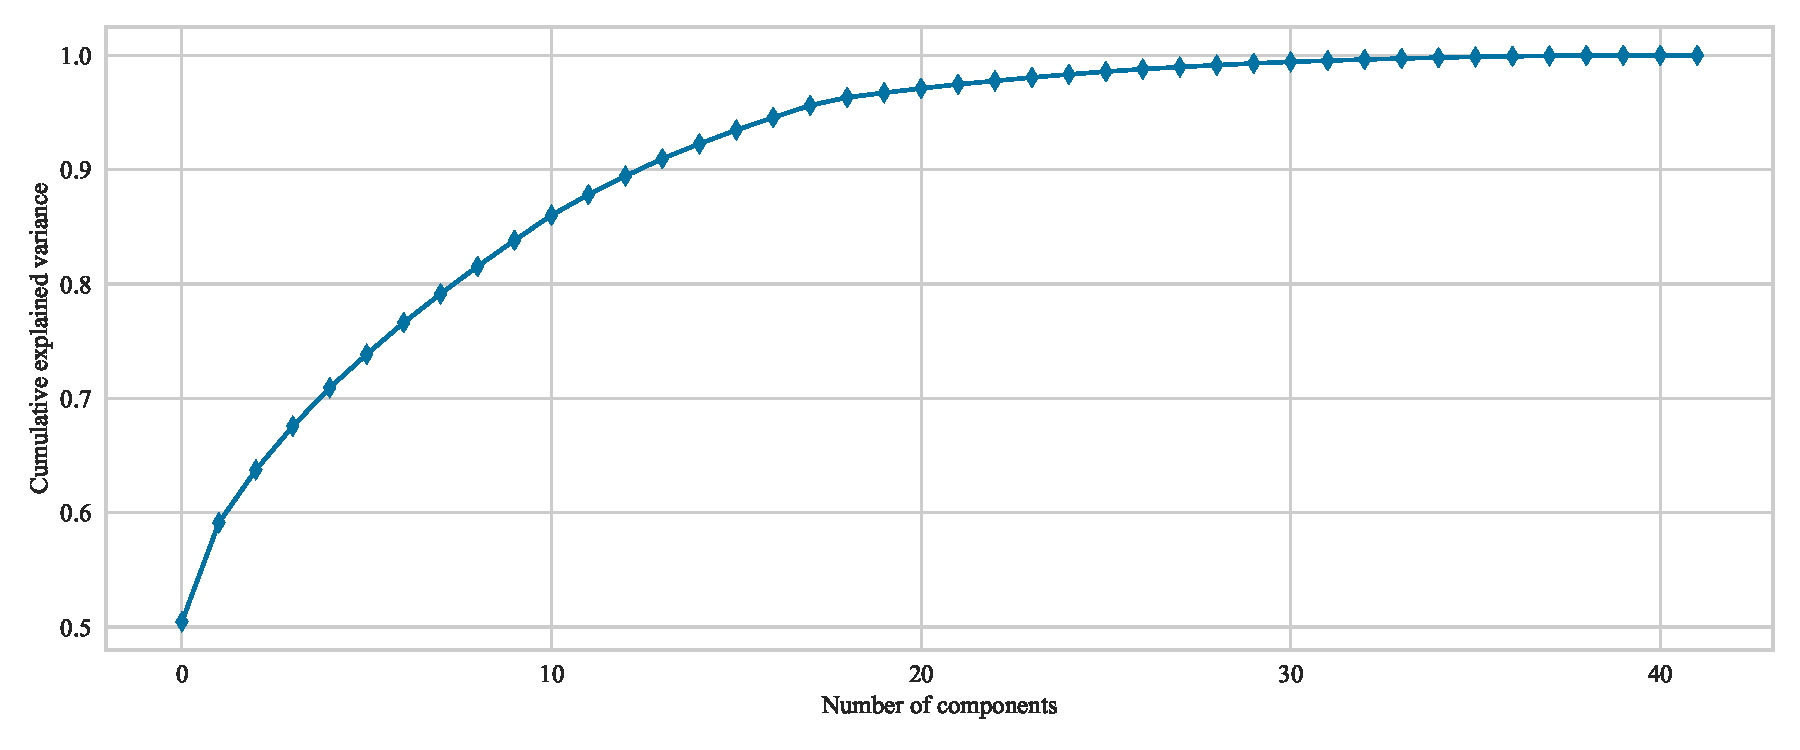
\includegraphics[width=1.0\linewidth]{[附件1]PCA累计解释方差图.pdf}
			\caption{语音业务指标累计解释方差}
			\label{fig:a1pca}
		\end{minipage}
		%\qquad
		\begin{minipage}{0.48\linewidth}
			\centering
			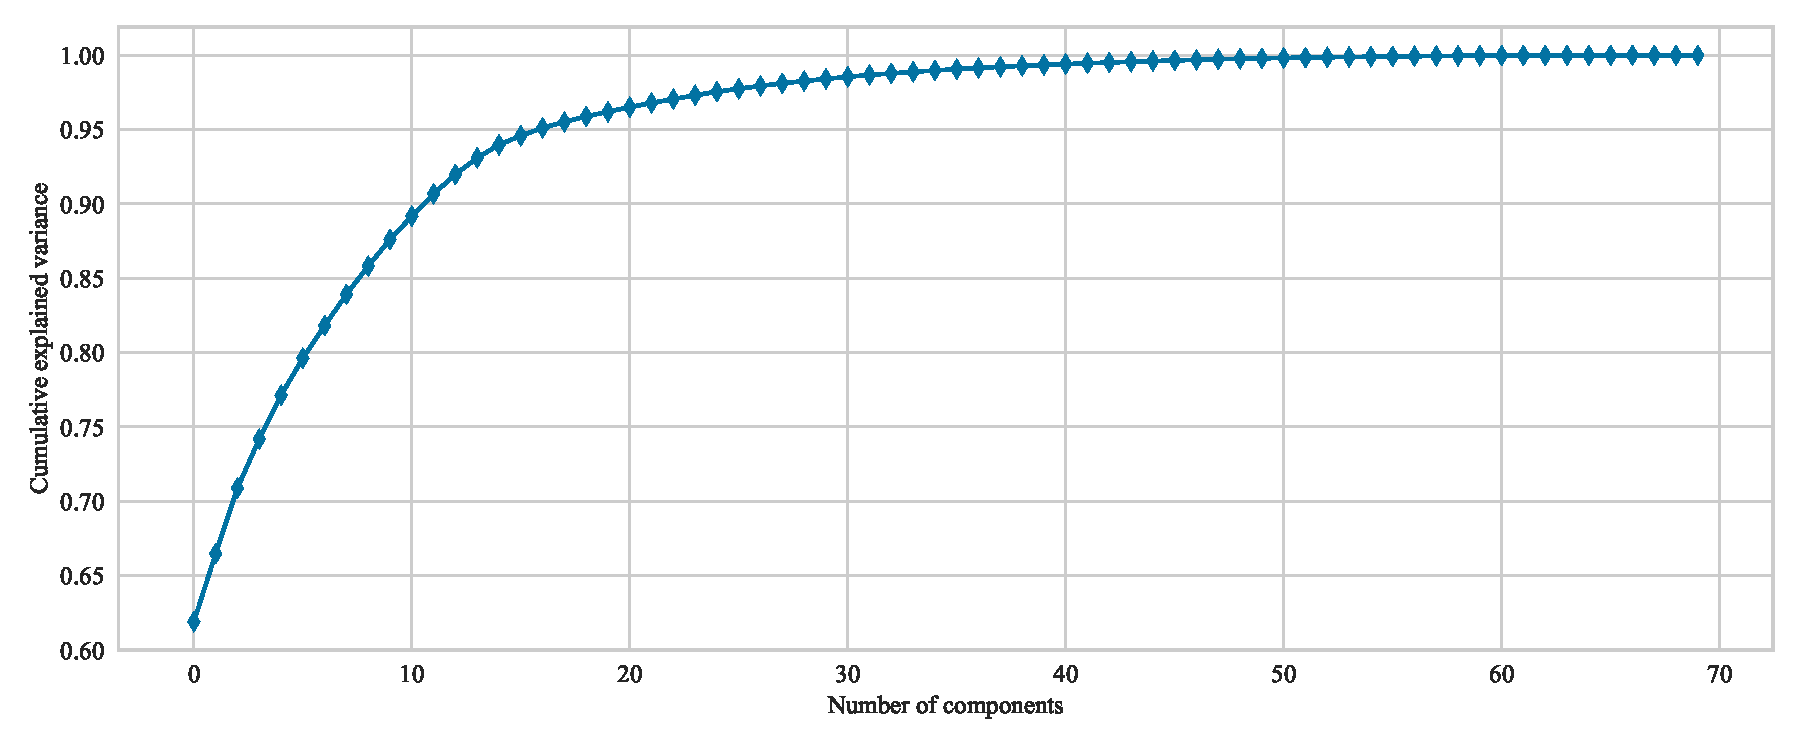
\includegraphics[width=1.0\linewidth]{[附件2]PCA累计解释方差图.pdf}
			\caption{上网业务指标累计解释方差}
			\label{fig:a2pca}
		\end{minipage}
	\end{figure}
	\begin{itemize}
		\item 对于\textbf{语音业务}:指标个数少于20个时,累计解释方差增幅较大,且约可累计解释$96\%$以上方差,在20个指标后,增幅较小,当指标个数为34个时,可解释近于$100\%$的方差。通过问题一的分析,我们可以将在其中量化结果中选择平均影响度量化值小于$0.0050$的进行特征剔除,包括:“是否关怀用户”、“是否投诉”、“高校”、“前3月ARPU”、“是否4G网络客户(本地剔除物联网)”;
		\item 对于\textbf{上网业务}:指标个数少于20个时,累计解释方差增幅较大,且约可累计解释$96\%$以上方差,在20个指标后,增幅较小,当指标个数为50个时,可解释近于$100\%$的方差。通过问题一的分析,我们可以将在其中量化结果中选择平均影响度量化值小于$0.0010$的进行特征剔除,包括:“和平精英”、“欢乐斗地主”、“其他,请注明.4”(视频类APP的特殊注明列)、“梦幻西游”、“穿越火线”、“炉石传说”、“部落冲突”、“梦幻诛仙”、“阴阳师”、“龙之谷”;
		\item 对于\textbf{剔除的因素的合理性分析}:综合问题分析,我们发现:这些因素在业务上的解释性较弱,且在量化结果中的影响度较小,且在PCA分析中,这些因素的累计解释方差较小,因此,我们认为这些因素对于业务的影响较小,故将其剔除分析。同时,我们对剔除前后的模型的准确率进行分析,发现,对于语音及上网业务的分析,模型准确率均有一定提升,介于$1.24\%\sim2.74\%$;
		\item 而对于下文\textbf{各个评分模型的建立}:我们会逐一分析,进行特征剔除,提升模型的准确性,以及模型的各项指标。上述的分析,首先在整体上确定合理方向。
	\end{itemize}

	\subsubsection{多种多分类模型的建立}
	\begin{itemize}
		\item \textbf{极端梯度提升(eXtreme Gradient Boosting, XGBoost)}。XGBoost算法是一种基于树模型的优化模型,其将弱分类器组合,训练出一个较强的分类器。该算法通过多次迭代,生成一个新的树模型用于优化前一个树模型,随着迭代次数的增多,该模型的预测精度也会相应提高\textcolor{blue}{\cite{pxgboost1}}。

		记通过数据处理后的数据集特征为$R\left(x_{ij}\right)_{m\times n}$,表示其包含$m$个用户,$n$个特征,在训练中形成的CART树的集合记为$F=\left\{f\left(x\right)=w_{q\left(x\right)},q:\mathbf{R}^n\to T,w\in \mathbf{R}^T\right\}$,其中$q$为树模型的叶节点决策规划,$T$为某一树模型叶节点数量,$w$为叶节点对应的得分\textcolor{blue}{\cite{pxgboost2}}。对于预测的$y$值,其计算公式为
		\begin{equation}
			\hat{y}=\varphi \left( x_i \right) =\sum\limits_{k=1}^K{f_k\left( x_i \right)} \label{fXGBoostypre}
		\end{equation}
	
		XGBoost算法在每一次迭代过程中会保存前面所学习的模型,会将这些模型加入到新一轮迭代过程中,因此我们记第$i$个模型为预测结果为
		\begin{equation}
			\hat{y}_{i}^{\left(t\right)}=\hat{y}_{i}^{\left(t-1\right)}+f_t\left(x_i\right) \label{fXGBoostyprei}
		\end{equation}
		
		XGBoost算法的目标函数计算公式如下
		\begin{equation}
			L^{\left(t\right)}=\sum\limits_{i=1}^{n}l\left(y_i,\hat{y}_{i}^{\left(t-1\right)}+f_t\left(x_i\right)\right)+\gamma T+\frac{1}{2}\lambda\sum\limits_{j=1}^T{w_j^2}+\mathrm{const} \label{fXGBoostL}
		\end{equation}
		% 其中
		% \begin{equation}
		% 	\Omega\left(f_t\right)=\gamma T+\frac{1}{2}\lambda\sum\limits_{j=1}^T{w_j^2} \label{fXGBoostOmega}
		% \end{equation}
		上述公式中,$l$为模型误差损失,描述在该模型下预测值与实际值之间的出差异损失,$\Omega$为模型叶节点的正则项惩罚系数,$\gamma$与$\lambda$为模型的超参数\textcolor{blue}{\cite{pxgboost2}}。
		通常情况下,我们难以用枚举法得到在模型中所训练出来的树结构,因此这里采用贪婪算法,从单叶子节点开始,通过迭代方法,将其加入到树结构中,从而得到最优解,其计算公式\textcolor{blue}{\cite{pxgboost3}}如下
		\begin{equation}
			\mathcal{L}_{split}=\frac{1}{2}\left[\frac{\left(\sum_{i\in I_L}g_i\right)^2}{\sum_{i\in I_L}h_i+\lambda}+\frac{\left(\sum_{i\in I_R}g_i\right)^2}{\sum_{i\in I_R}h_i+\lambda}-\frac{\left(\sum_{i\in I}g_i\right)^2}{\sum_{i\in I}h_i+\lambda}\right]-\gamma \label{fXGBoostLsplit}
		\end{equation}
		其中$I_j=\left\{i|q\left(x_i\right)=j\right\}$为叶节点$j$上的样本集合\textcolor{blue}{\cite{pxgboost2}},且有
		\begin{equation}
			g_i=\partial_{\hat{y}^{\left(t-1\right)}}l\left(y_i,\hat{y}_i^{\left(t-1\right)}\right)\qquad h_i=\partial_{\hat{y}^{\left(t-1\right)}}^2l\left(y_i,\hat{y}_i^{\left(t-1\right)}\right) \label{xgboostgihi}
		\end{equation}
		% \begin{equation}
		% 	h_i=\partial_{\hat{y}^{\left(t-1\right)}}^2l\left(y_i,\hat{y}_i^{\left(t-1\right)}\right) \label{xgboosthi}
		% \end{equation}
	
		通过上述分析,我们可以得到XGBoost算法简图,如\textcolor{blue}{\cref{fig:XGBoost}}所示。
		\begin{figure}[h!t]
			\centerline{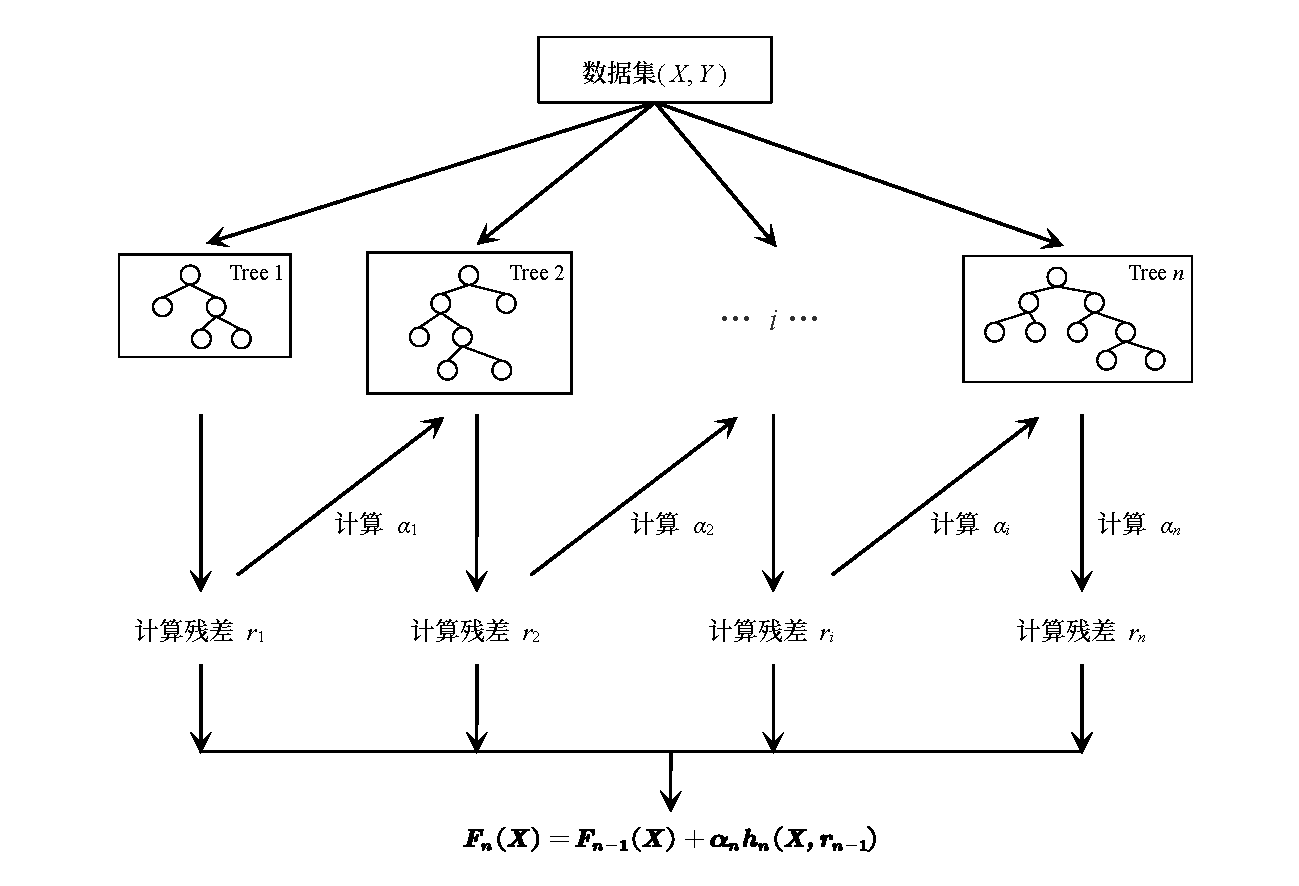
\includegraphics[scale=0.60]{XGBoost简图.pdf}}
			\caption{XGBoost算法简图}\label{fig:XGBoost}
		\end{figure}
		\item \textbf{K-近邻(K Nearest Neighbor, KNN)}。KNN算法的主要思想为:在出现新样本时从现有的训练数据中找到与其相对应的最接近的$K$个样本,并根据最相似的类别出现的样本进行分类。基于多数$K$个样本所属的类别来分辨待分类的数据集所属的类别\textcolor{blue}{\cite{pknn}}。接近度由两点之间的距离函数给出属性空间中的点决定。距离函数通常使用两个点之间的标准欧几里得距离。欧氏距离的计算公式如下
		\begin{equation}
			d(X, Y)=\sqrt{\sum\limits_{i=1}^{n}\left(X_{i}-Y_{i}\right)^{2}} \label{fdistance}
		\end{equation}
		其中$X=\left(x_{1},x_{2},\cdots,x_{m}\right)^{\mathrm{T}}$和$Y=\left(y_{1},y_{2},\cdots,y_{m}\right)^{\mathrm{T}}$表示两个样本列数据,$m$为样本数量。
		
		\item \textbf{支持向量机(Support Vector Machine, SVM)}。SVM建立在结构风险最小原理及Vapnik-Chervonenkis理论基础之上\textcolor{blue}{\cite{psvm}},以有限的数据信息,在数据样本中找出合适区分类别的决策分界面,且保证边界点与分界面尽可能远,即需要再找出合适的边界分界面,该算法示意图如\textcolor{blue}{\cref{fig:svmpicture}}所示。
		\begin{figure}[h!t]
			\centerline{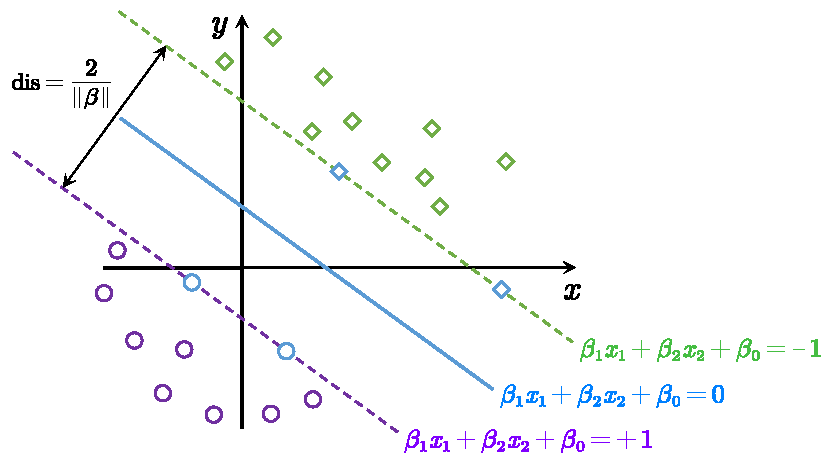
\includegraphics[scale=0.88]{SVM示意图.pdf}}
			\caption{SVM示意图}\label{fig:svmpicture}
		\end{figure}
		而由于SVM多应用于解决二分类问题,且我们需要建立多分类模型,因此需要对其进行相应的改进。本文采用OVR(One Versus Rest)方法,将该问题改进为多个二分类问题\textcolor{blue}{\cite{psvm}}。在模型的训练时,任意将某一类别记为一类,其余类别记为另一类别,依次下去,建立出多分类的SVM模型。而对于核函数的选择,本文选择高斯核函数进行求解,其定义公式如下
		\begin{equation}
			K\left(x_i, x_j\right)=\exp \left(-\frac{\left\|x_i-x_j\right\|^{2}}{2\sigma^{2}}\right)=\exp \left(-\gamma \left\|x_i-x_j\right\|^{2}\right) \label{fgauss}
		\end{equation}
		对于高斯核函数,其可以反映出样本两点之间的相似度大小。当$\sigma$确定后,若两点之间距离越小,则相似度趋近于1;若距离越大,则相似度趋近于0。
		\item \textbf{LightGBM(Light Gradient Boosting Machine)}。LightGBM模型是基于决策树算法构建的一种高效的机器学习算法\textcolor{blue}{\cite{plightgbm}}。其为XGBoost、直方图算法(Histogram)、基于梯度的单边采样(GOSS)算法以及互斥特征捆绑(EFB)算法的结合的一种算法。
		
		\item \textbf{多分类逻辑回归(Multinomial Logistic Regression)}。多分类逻辑回归是基于逻辑回归(Logistic Regression)进行学习的分类模型。对于逻辑回归模型,其属于分类模型,多用于二分类问题。若数据集为$\left(\boldsymbol{A},\boldsymbol{B}\right)=\left(\left(\boldsymbol{a}_1,b_1\right),\left(\boldsymbol{a}_2,b_2\right),\cdots,\left(\boldsymbol{a}_m,b_m\right)\right)^{\mathrm{T}}$,其中$\boldsymbol{a}_i=\left(a_i^1,a_i^2,\cdots,a_i^j\right)$,$a_i^j$为样本$\boldsymbol{a}_i$的第$j$个特征,$\boldsymbol{B}$为因变量标签矩阵,该模型使用Sigmoid函数,同时构建样本$\boldsymbol{a}_i$所属类别的概率,对于标签为$1$的结果,其概率可写为
		\begin{equation}
			P\left(b_i=1\mid \boldsymbol{a}_i,\boldsymbol{\omega}\right)=\frac{1}{1+\mathrm{e}^{-\boldsymbol{a}_ib_i\boldsymbol{\omega}^\mathrm{T}}} \label{fLRp}
		\end{equation}
		其中$\boldsymbol{\omega}=\left(\omega^0,\omega^1,\cdots,\omega^n\right)^\mathrm{T}$为权重向量,即为优化模型的超参数。
		逻辑回归中利用损失函数来评估模型的预测结果与实际值之间的误差,其计算公式如下
		\begin{equation}
			L\left(\boldsymbol{A},\boldsymbol{B},\boldsymbol{\omega}\right)=\frac{1}{m}\sum\limits_{i=1}^{m}\log \left(1+\mathrm{e}^{-\boldsymbol{a}_ib_i \boldsymbol{\omega}^{\mathrm{T}}}\right) \label{fLRl}
		\end{equation}
		而对于$\boldsymbol{\omega}$,常采用梯度下降法来获得模型参数的最优解,其通过
		\begin{equation}
			\boldsymbol{\omega}^{\alpha+1}=\boldsymbol{\omega}^\alpha-\frac{\gamma}{m}\sum\limits_{i=1}^{m}\left(\frac{1}{1+\mathrm{e}^{-\boldsymbol{a}_ib_i \boldsymbol{\omega}^{\mathrm{T}}}}-1\right)\boldsymbol{a}_ib_i \label{fLRw}
		\end{equation}
		进行迭代更新,其中$\gamma$为模型的学习率,当$\left|  \boldsymbol{\omega}^{\alpha}-\boldsymbol{\omega}^{\alpha+1} \right|<\eta$或达到最大迭代次数时,停止训练,输出最终模型,其中$\eta$为人为给定的阈值\textcolor{blue}{\cite{plr}}。
	\end{itemize}
	
	\subsubsection{Stacking集成学习原理解释}
	Stacking集成学习是通过建立多个机器学习模型,将其有目的地进行合理组合,从各模型中学到优点,有利于模型的效果的提升。其基本过程为,首先将已经经过处理的原数据集划分成若干个子集数据,在第一层建立多个模型的融合模型,输入数据,并采用五折交叉验证,获得每个模型的对于因变量标签的预测结果;之后第一层的输出结果作为第二层较弱分类模型的输入数据,第二层单个模型进行训练学习,得到最终预测结果\textcolor{blue}{\cite{pstacking}}。算法示意图如\textcolor{blue}{\cref{fig:StackingPicture}}所示,算法伪代码如\textcolor{blue}{Algorithm\ref{StackingFunciton}}所示。

	\scalebox{0.88}{
	\begin{algorithm}[H]
		\label{StackingFunciton}
		\KwIn{训练集$\mathcal{D}$\

		第一层学习模型$\mathcal{F}_1$,$\mathcal{F}_2$,$\cdots$,$\mathcal{F}_n$\

		第二层学习模型$\mathcal{S}$}
		\For{$t=1,2,3,\cdots,n$}{$h_n=\mathcal{F}_n\left(\mathcal{D}\right)$}
		$\mathcal{D}'=\varnothing$\

		\For{$i=1,2,\cdots,m$}{\For{$t=1,2,\cdots,n$}{$z_{in}=h_n\left(x_i\right)$}
		$\mathcal{D}'=\mathcal{D}'\cup\left(\left(z_{i1},z_{i2},\cdots,z_{in}\right),y_i\right)$}
		$h'=\mathcal{S}\left(D'\right)$

		\KwOut{$\mathcal{H}\left(x\right)=h'\left(h_1\left(x\right),h_2\left(x\right),\cdots,h_n\left(x\right)\right)$}
		\caption{Stacking集成学习}
	\end{algorithm}}
	\begin{figure}[H]
		\centerline{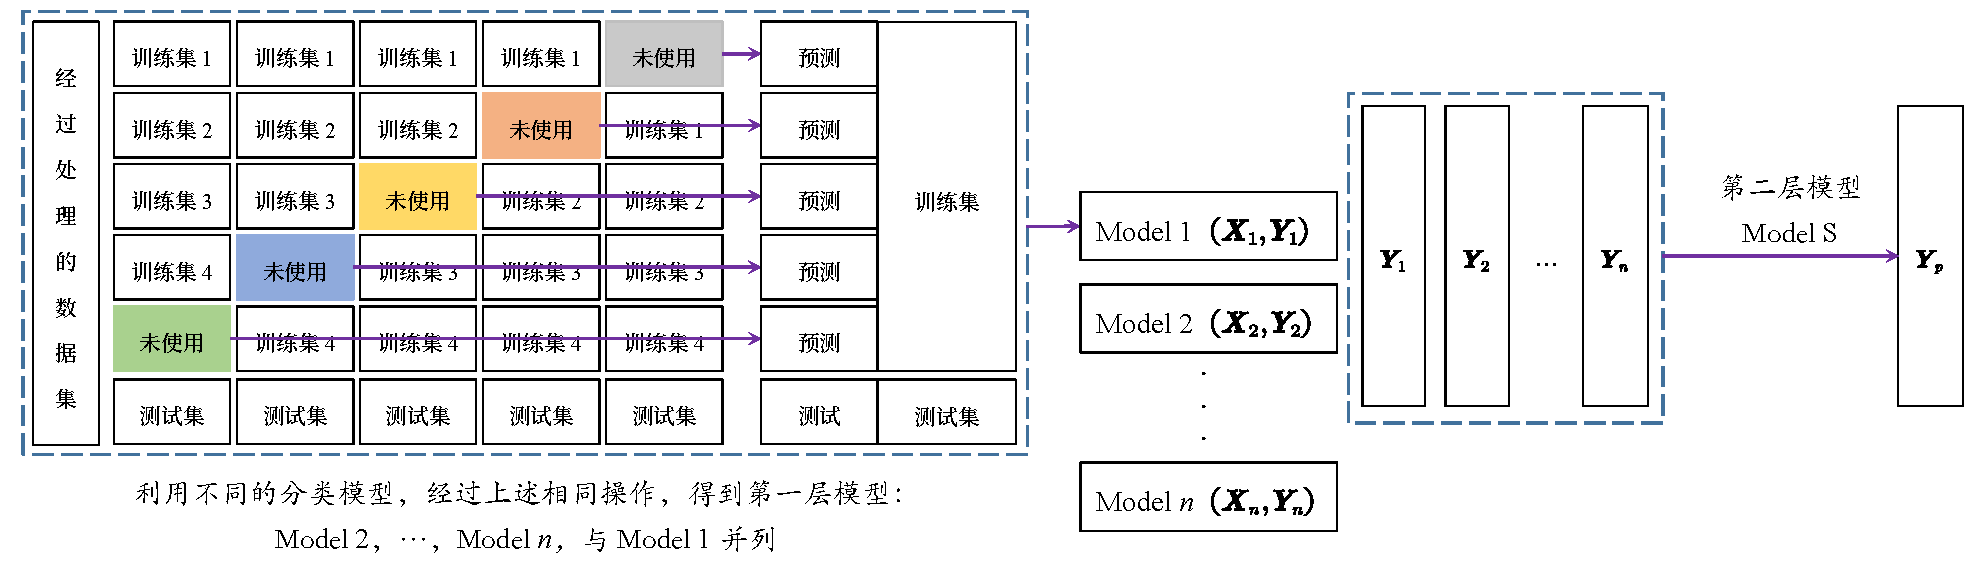
\includegraphics[scale=0.56]{Stacking示意图.pdf}}
		\caption{Stacking集成学习示意图}\label{fig:StackingPicture}
	\end{figure}

	\subsubsection{模型的超参数调优}
	为了更好地预测用户评分,我们在建立上述模型的基础上,对模型进行超参数调优,以提高模型的预测准确性,减小平均绝对误差以及均方误差。
	\begin{itemize}
		\item \textbf{随机森林调优}:这边我们以语音业务中“网络覆盖与信号强度”评分为研究对象,进行调参,其他评分下建立的模型调参与此大致相同。随机森林最需要调节的参数为树的棵数(n\_estimators),而森林深度、信息计算方法、叶节点等为辅助调参参数。首先我们绘制模型“Acc-n\_estimators”图像,见\textcolor{blue}{\cref{fig:a1RFturningF}},图像纵坐标为模型准确率,横坐标为n\_estimators值。
		\begin{figure}[htbp]
			\centerline{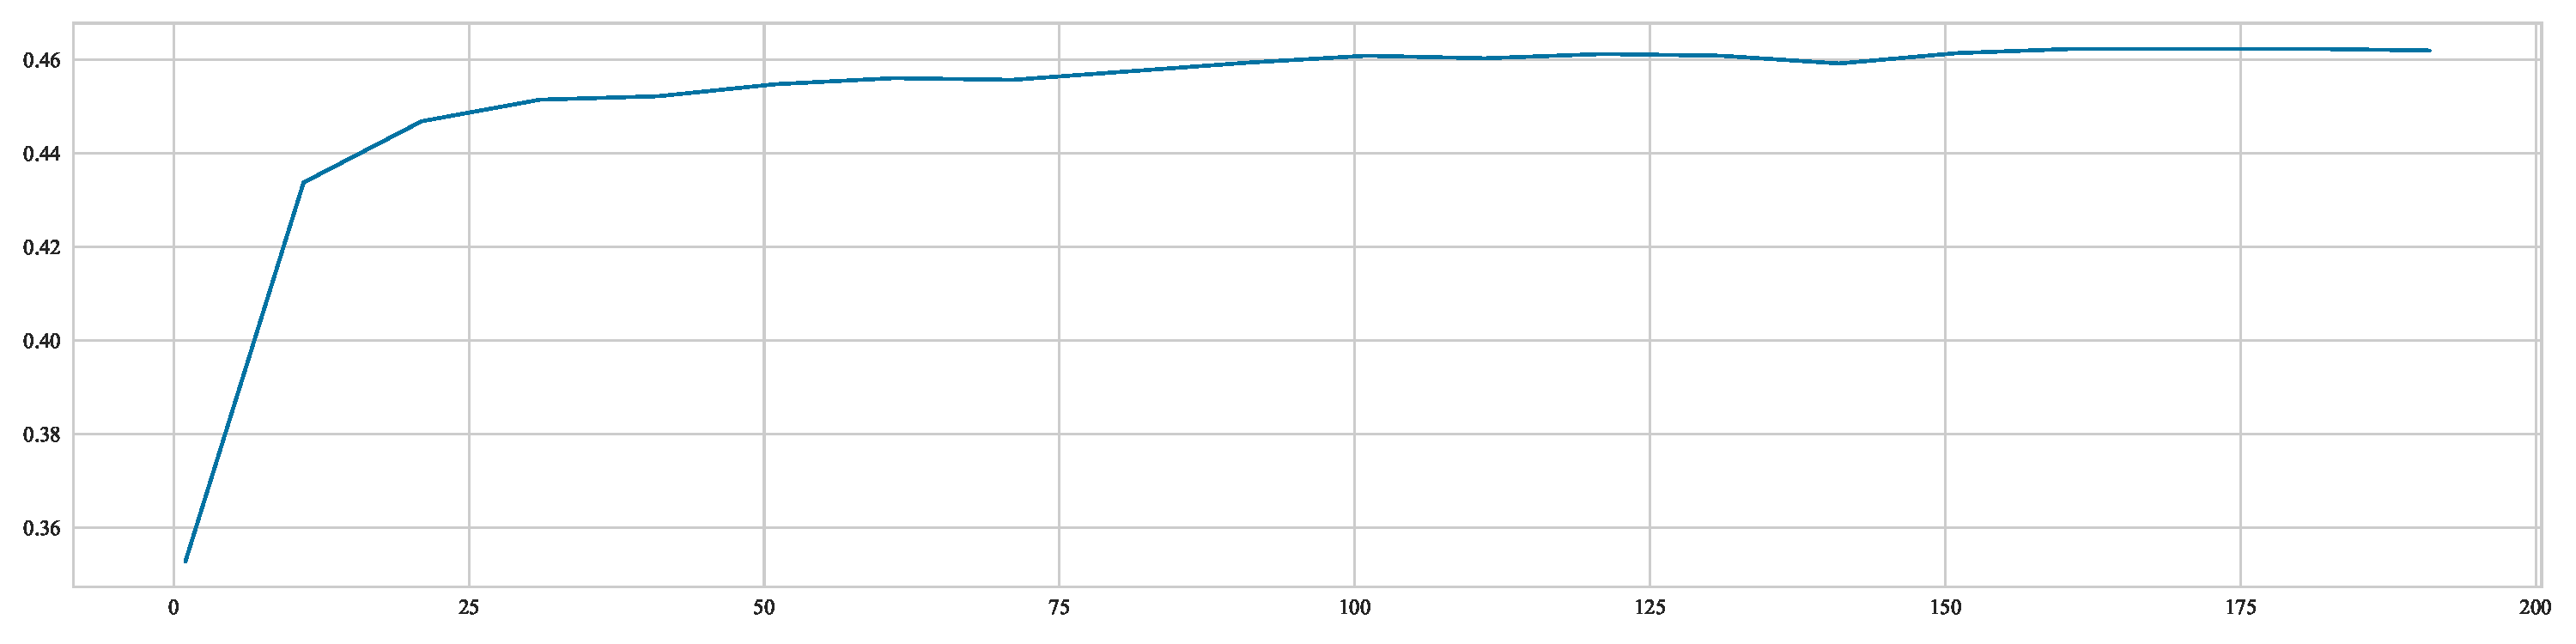
\includegraphics[scale=0.24]{[附件1]随机森林调参F.pdf}}
			\caption{随机森林n\_estimators调优图像,第一次}\label{fig:a1RFturningF}
		\end{figure}	
		\begin{figure}[htbp]
			\centerline{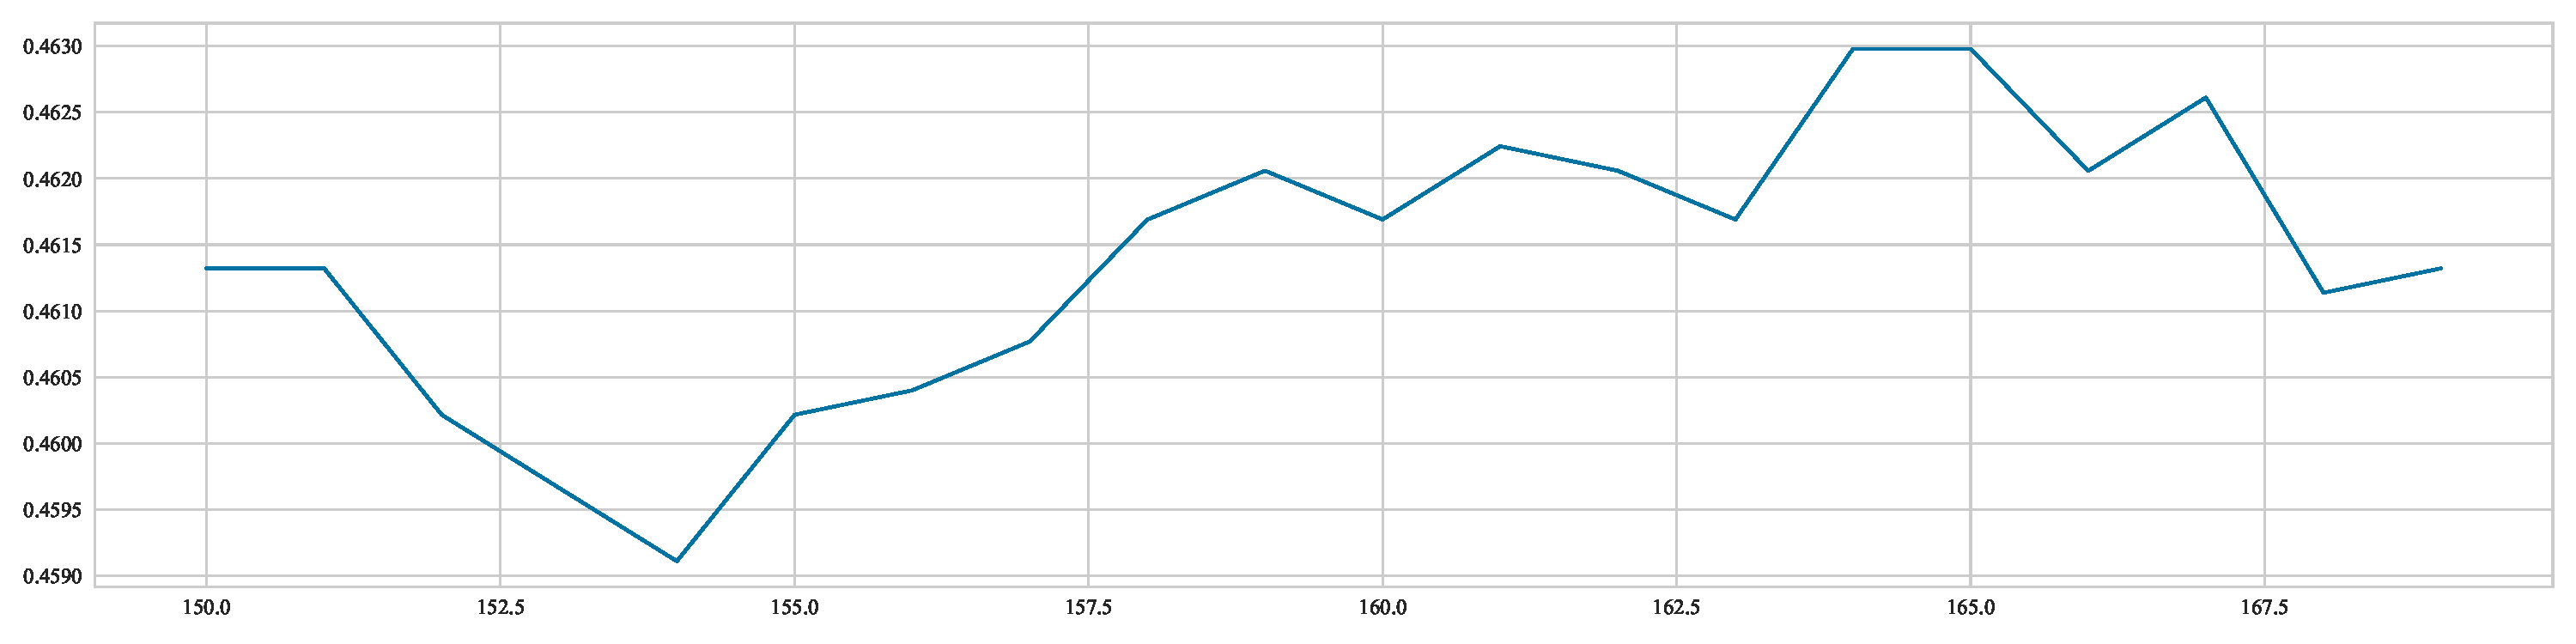
\includegraphics[scale=0.24]{[附件1]随机森林调参S.pdf}}
			\caption{随机森林n\_estimators调优图像,第二次}\label{fig:a1RFturningS}
		\end{figure}
		通过观察可以发现,该模型对于该数据在n\_estimators=161附近时,准确率最高,故我们选择n\_estimators=161作为参数值。根据上述分析结果,进一步细化随机森林学习曲线,我们将在$150\sim170$之间寻找最佳值。我们绘制出n\_estimators在$150\sim170$之间的学习曲线,见\textcolor{blue}{\cref{fig:a1RFturningS}}。通过观察该图,我们发现对于该数据集,该模型的n\_estimators最佳值为164,故我们选择n\_estimators=164作为参数值。

		之后我们对参数max\_features,min\_samples\_leaf,criterion,max\_depth利用Python的sklearn.model\_selection中的GridSearchCV模块进行调节,最终得到在该评分下,随机森林模型最优参数,结果见\textcolor{blue}{\cref{tab:a1RFturning}}。
		\begin{table}[htbp]
			\centering
			\caption{语音业务-网络覆盖与信号强度评分下随机森林模型最优参数}
			\setlength{\aboverulesep}{0pt}
			\setlength{\belowrulesep}{0pt}
			\scalebox{0.88}{
				\begin{tabular}{cc}
				\toprule
				\textbf{参数} & \textbf{最优选取} \\
				\midrule
					n\_estimators & 164 \\
					max\_features & log2 \\
					min\_samples\_leaf & 8 \\
					criterion & gini \\
					max\_depth & 19 \\
				\bottomrule
				\end{tabular}}
			\label{tab:a1RFturning}
		\end{table}
		
		通过计算,该模型调参前准确率为$45.67\%$,调节最优参数后,准确率上升至$51.01\%$,较原先提升了$11.69\%$,可以发现,调参效果良好。
		\item \textbf{XGBoost、KNN、SVM、LightGBM、多分类逻辑回归调优}:对于这些模型,我们采用网格搜索的方法进行调参,设置好需要调参的对象及范围,利用Python的sklearn库中的model\_selection.GridSearchCV模块,进行调优。具体代码可以参看附录[D]。通过分析,可以发现,各个模型在调参后,准确率均有一定提升,较原模型准确率的提升部分模型可以达到$14.25\%$,提升的百分点约为$6.28\%$,调参效果良好,符合预期效果。
	\end{itemize}

	\subsubsection{特征选择}
	为了更好地预测用户评分,尽可能地提升模型的准确率、泛化能力,以及降低其预测的平均绝对误差、均方误差,我们在问题一的基础上,对特征进行了筛选,并且结合XGBoost模型的特种重要性可视化进行综合分析。对语言及上网业务共计八项评分,每一个进行了综合特征筛选。这里我们以语音业务-语音通话整体满意度评分为例,进行特征选择的分析。根据XGBoost模型,我们绘制出该评分下影响因素的重要性可视化图,如\textcolor{blue}{\cref{fig:a1FirstXGBoost}}所示。\textcolor{blue}{\footnote{其中由于上网业务的特征较多,对于其下的四项评分,我们仅选取了20个特征进行了可视化,但对评分特征选择的分析,本文是对所有特征进行选择的。}}
	\begin{figure}[htbp]
		\centerline{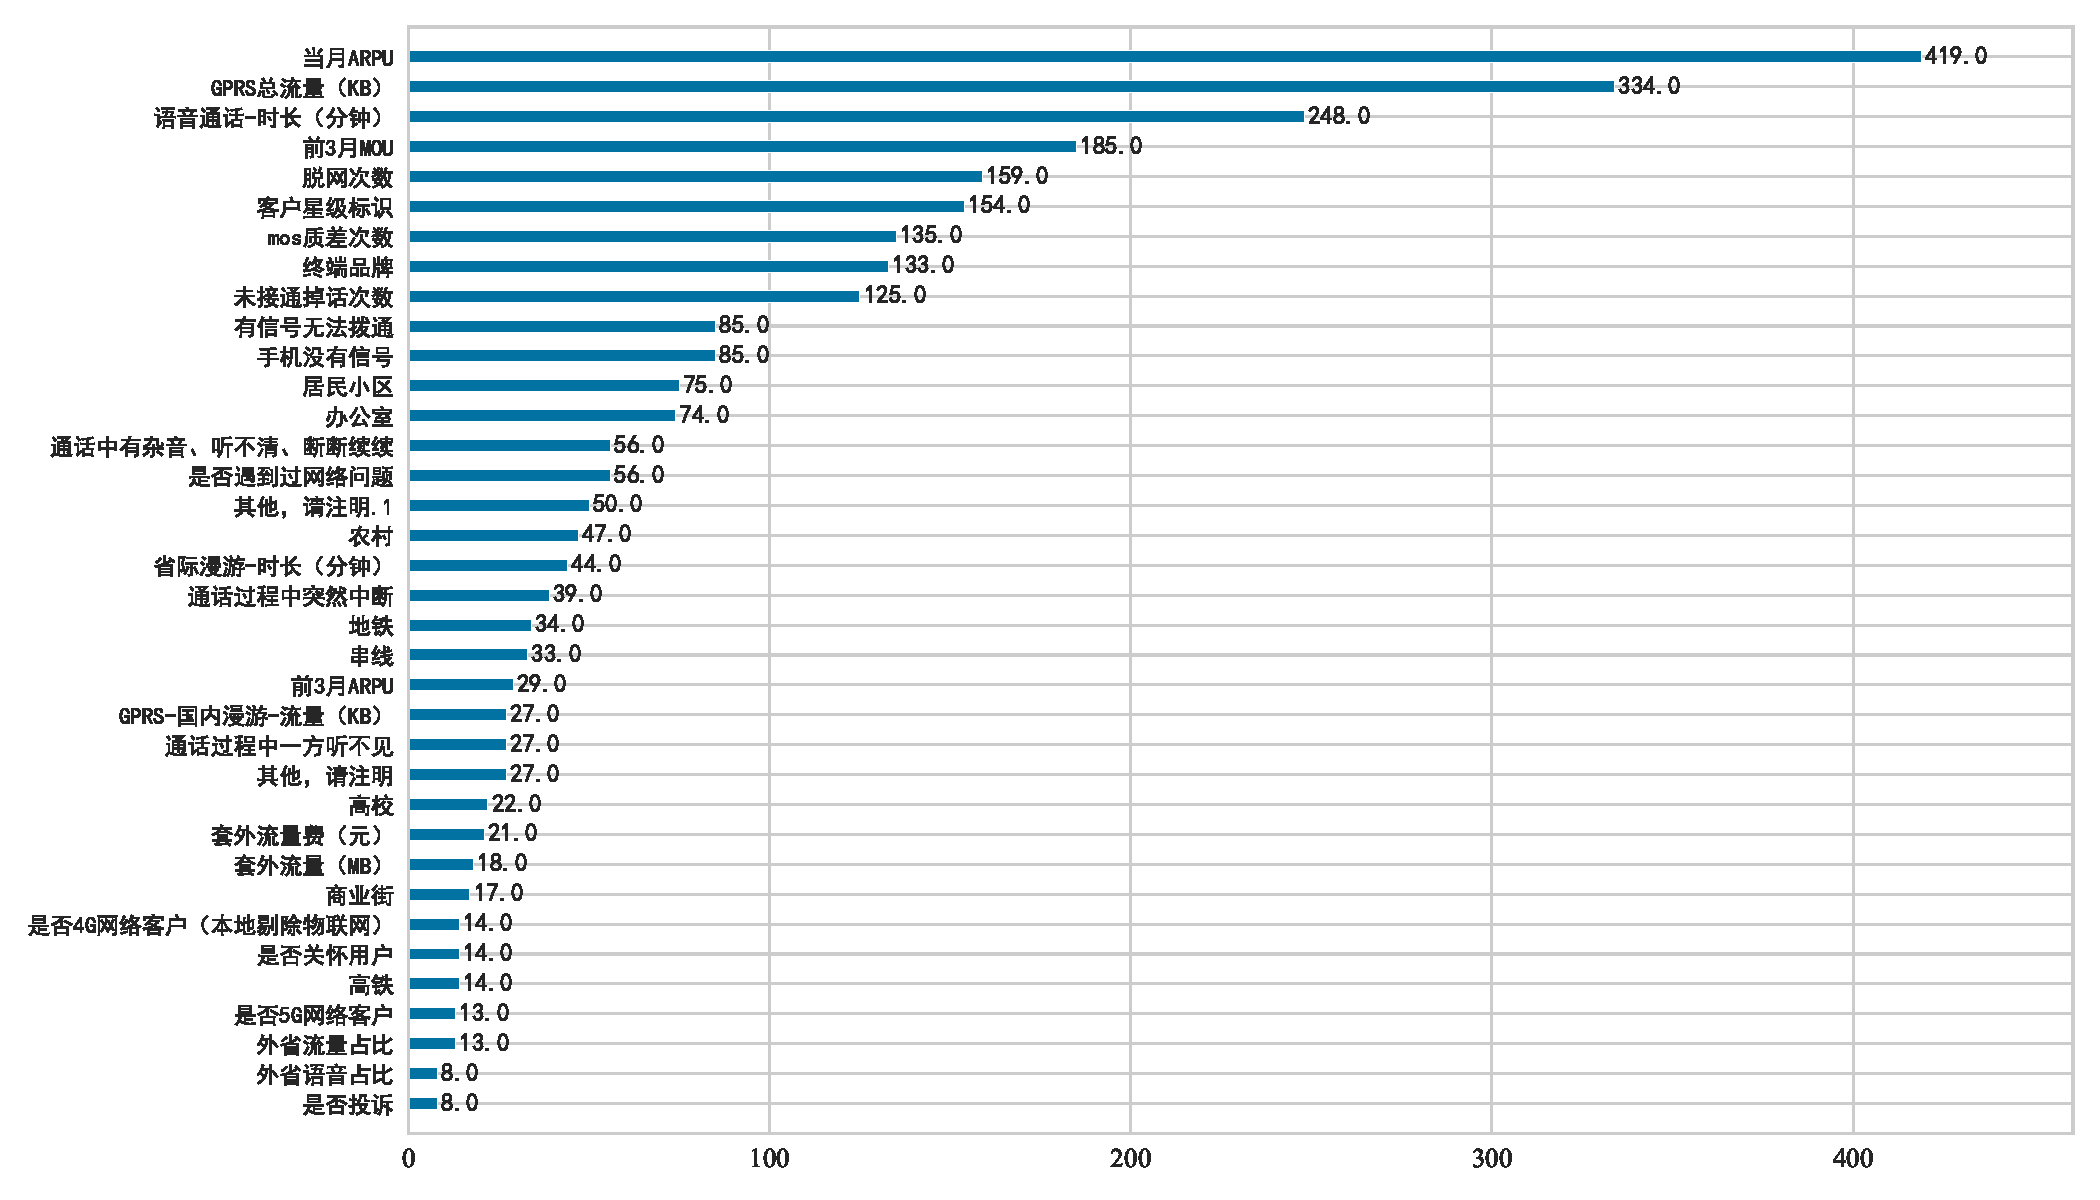
\includegraphics[scale=0.34]{[附件1]语音通话整体满意度各项指标重要程度(XGBoost,F-score).pdf}}
		\caption{语音通话整体满意度各项指标重要程度,XGBoost}\label{fig:a1FirstXGBoost}
	\end{figure}

	观察该图,我们可以发现,对于语音业务的语音通话整体满意度评分的影响因素,XGBoost模型计算的结果与随机森林模型大致相似。我们综合\textcolor{blue}{\cref{tab:a1allquantization}}以及\textcolor{blue}{\cref{fig:a1FirstXGBoost}}结果,选择两个模型分析出的重要性高的特征,且剔除随机森林模型量化结果在$0.0010$以下,以及XGBoost模型量化结果在$10$以下的特征,它们为:“是否4G网络客户(本地剔除物联网)”、“外省语音占比”、“是否投诉”三项,并在这基础上建立后续模型,进行分析、预测。

	而对于语音及上网业务的其余评分,思路与上述一致,由于篇幅原因,这里不再赘述。对于各评分的XGBoost特征重要性可视图,读者可以在附件中查看,见\textcolor{blue}{\cref{fig:a1SecondXGBoost}}\textasciitilde\textcolor{blue}{\cref{fig:a2FourthXGBoost}}。
	\subsubsection{模型的选择及集成}
	对八项评分,我们均建立\textbf{随机森林、XGBoost、KNN、SVM、LightGBM、多分类逻辑回归}模型,且进行参数调优,得到每一个最优模型。并且计算每一个模型的准确率(Accuracy)、平均绝对误差(Mean Absolute Error,MAE)、均方误差(Mean Square Error, MSE)。对于多分类模型,该三项指标,计算公式如下:
	\begin{itemize}
		\item \textbf{准确率}
			\begin{equation}
			\mathrm{Accuracy}=\frac{N_{\mathrm{TruePredict}}}{N_{\mathrm{Sample}}} \label{Accuracy}
			\end{equation}
		其中,$N_{\mathrm{TruePredict}}$为预测正确的样本数,$N_{\mathrm{Sample}}$为被预测的样本总数;
		\item \textbf{平均绝对误差}
			\begin{equation}
			\mathrm{MAE}=\frac{1}{n}\sum_{i=1}^{n}\left|y_{i}-\hat{y}_{i}\right| \label{MAE}
			\end{equation}
		其中,$y_i$为实际值,$\hat{y}_i$为预测值;
		\item \textbf{均方误差}
			\begin{equation}
			\mathrm{MSE}=\frac{1}{n}\sum_{i=1}^{n}\left(y_{i}-\hat{y}_{i}\right)^{2} \label{MSE}
			\end{equation}
	\end{itemize}
	利用上述公式,我们可以计算出每个模型这三项指标,结果见\textcolor{blue}{\cref{tab:RFXGBoost}}、\textcolor{blue}{\cref{tab:KNNSVM}}以及\textcolor{blue}{\cref{tab:LightGBMLR}}。
	\begin{table}[H]
	\centering
	\caption{随机森林、XGBoost各评分三项指标结果}
	\setlength{\aboverulesep}{0pt}
	\setlength{\belowrulesep}{0pt}
	\scalebox{0.76}{
	  \begin{tabular}{ccccccc}
	  \toprule
	  \multirow{2}[4]{*}{\textbf{评分项目}} & \multicolumn{3}{c}{\textbf{随机森林}} & \multicolumn{3}{c}{\textbf{XGBoost}} \\
  \cmidrule{2-7}          & \textbf{准确率} & \textbf{平均绝对误差} & \textbf{均方误差} & \textbf{准确率} & \textbf{平均绝对误差} & \textbf{均方误差} \\
	  \midrule
	  语音通话整体满意度 & 0.5829  & 1.2910  & 6.5378  & 0.5949  & 1.2320  & 6.0331  \\
	  网络覆盖与信号强度 & 0.5101  & 1.5304  & 7.6077  & 0.4936  & 1.4926  & 7.0562  \\
	  语音通话清晰度 & 0.5424  & 1.2864  & 6.0691  & 0.5331  & 1.3039  & 6.0976  \\
	  语音通话稳定性 & 0.5184  & 1.3996  & 6.5433  & 0.5184  & 1.4282  & 6.7928  \\
	  \midrule
	  手机上网整体满意度 & 0.4459  & 1.7692  & 8.6752  & 0.4359  & 1.7222  & 8.2265  \\
	  网络覆盖与信号强度 & 0.3903  & 1.7322  & 7.5214  & 0.3775  & 1.7863  & 7.8775  \\
	  手机上网速度 & 0.3775  & 1.7892  & 7.7664  & 0.3533  & 1.7222  & 6.9587  \\
	  手机上网稳定性 & 0.3803  & 1.8348  & 8.0912  & 0.3889  & 1.7792  & 7.8846  \\
	  \bottomrule
	  \end{tabular}}
	\label{tab:RFXGBoost}
  	\end{table}
	\begin{table}[H]
	\centering
	\caption{KNN、SVM各评分三项指标结果}
	\setlength{\aboverulesep}{0pt}
	\setlength{\belowrulesep}{0pt}
	\scalebox{0.76}{
	  \begin{tabular}{ccccccc}
	  \toprule
	  \multirow{2}[4]{*}{\textbf{评分项目}} & \multicolumn{3}{c}{\textbf{KNN}} & \multicolumn{3}{c}{\textbf{SVM}} \\
  \cmidrule{2-7}          & \textbf{准确率} & \textbf{平均绝对误差} & \textbf{均方误差} & \textbf{准确率} & \textbf{平均绝对误差} & \textbf{均方误差} \\
	  \midrule
	  语音通话整体满意度 & 0.5893  & 1.2680  & 6.5055  & 0.5884  & 1.3582  & 7.3103  \\
	  网络覆盖与信号强度 & 0.5009  & 1.5506  & 7.6924  & 0.4991  & 1.5948  & 8.0571  \\
	  语音通话清晰度 & 0.5543  & 1.3002  & 6.2063  & 0.5543  & 1.3932  & 7.1133  \\
	  语音通话稳定性 & 0.5239  & 1.4162  & 6.7385  & 0.5267  & 1.4678  & 7.2652  \\
	  \midrule
	  手机上网整体满意度 & 0.4217  & 1.8148  & 8.6268  & 0.4330  & 1.8575  & 9.3846  \\
	  网络覆盖与信号强度 & 0.3946  & 1.7792  & 8.0271  & 0.3960  & 1.8504  & 8.6966  \\
	  手机上网速度 & 0.3818  & 1.7806  & 7.7094  & 0.3732  & 1.8519  & 8.5071  \\
	  手机上网稳定性 & 0.3832  & 1.7977  & 8.1054  & 0.3818  & 1.9259  & 9.0057  \\
	  \bottomrule
	  \end{tabular}}
	\label{tab:KNNSVM}
  	\end{table}
	\begin{table}[H]
	\centering
	\caption{LightGBM、多分类逻辑回归各评分三项指标结果}
	\setlength{\aboverulesep}{0pt}
	\setlength{\belowrulesep}{0pt}
	\scalebox{0.76}{
	  \begin{tabular}{ccccccc}
	  \toprule
	  \multirow{2}[4]{*}{\textbf{评分项目}} & \multicolumn{3}{c}{\textbf{LightGBM}} & \multicolumn{3}{c}{\textbf{多分类逻辑回归}} \\
  \cmidrule{2-7}          & \textbf{准确率} & \textbf{平均绝对误差} & \textbf{均方误差} & \textbf{准确率} & \textbf{平均绝对误差} & \textbf{均方误差} \\
	  \midrule
	  语音通话整体满意度 & 0.5737  & 1.2366  & 5.8131  & 0.5829  & 1.2330  & 6.0230  \\
	  网络覆盖与信号强度 & 0.4899  & 1.5037  & 7.1298  & 0.5000  & 1.4797  & 7.0101  \\
	  语音通话清晰度 & 0.5396  & 1.2606  & 5.6860  & 0.5451  & 1.2845  & 5.9843  \\
	  语音通话稳定性 & 0.5110  & 1.3517  & 6.1455  & 0.5285  & 1.3923  & 6.5727  \\
	  \midrule
	  手机上网整体满意度 & 0.4444  & 1.7123  & 8.1852  & 0.4302  & 1.7821  & 8.7365  \\
	  网络覆盖与信号强度 & 0.3846  & 1.7393  & 7.4772  & 0.3718  & 1.8547  & 8.4530  \\
	  手机上网速度 & 0.3704  & 1.7222  & 7.2464  & 0.3761  & 1.8219  & 8.0840  \\
	  手机上网稳定性 & 0.3675  & 1.8433  & 8.1140  & 0.3818  & 1.8305  & 8.2550  \\
	  \bottomrule
	  \end{tabular}}
	\label{tab:LightGBMLR}
  	\end{table}
	通过分析上述表格,我们综合模型的准确率、平均绝对误差、均方误差的表现,对每一项评分选择基模型以及第二层模型,选择好的组合见\textcolor{blue}{\cref{tab:StackingChoose}}。
	\begin{table}[H]
	\centering
	\caption{各个评分预测Stacking集成学习模型的建立}
	\setlength{\aboverulesep}{0pt}
	\setlength{\belowrulesep}{0pt}
	\scalebox{0.78}{
	  \begin{tabular}{ccccccc}
	  \toprule
	  \textbf{评分项目} & \multicolumn{5}{c}{\textbf{基模型}}      & \textbf{第二层模型} \\
	  \midrule
	  语音通话整体满意度 & XGBoost & KNN   & SVM   & LightGBM & LR    & RF \\
	  网络覆盖与信号强度 & RF    & XGBoost & KNN   & SVM   & LR    & LightGBM \\
	  语音通话清晰度 & XGBoost & KNN   & SVM   & LightGBM & LR    & RF \\
	  语音通话稳定性 & RF    & SVM   & KNN   & LightGBM & LR    & XGBoost \\
	  \midrule
	  手机上网整体满意度 & RF    & XGBoost & KNN   & LightGBM & LR    & SVM \\
	  网络覆盖与信号强度 & RF    & XGBoost & KNN   & LightGBM & LR    & SVM \\
	  手机上网速度 & RF    & XGBoost & KNN   & LightGBM & LR    & SVM \\
	  手机上网稳定性 & RF    & XGBoost & KNN   & LightGBM & LR    & SVM \\
	  \bottomrule
	  \end{tabular}}
	\label{tab:StackingChoose}
 	\end{table}
	
	依据\textcolor{blue}{\cref{tab:StackingChoose}}的融合组合,我们最终建立对于语音及上网业务每一项评分的用户评分预测模型,用于对附件2以及附件4中的用户评分进行预测。
	\subsubsection{客户评分预测}
	在“5.1 数据的准备”中,我们提到对学习数据与预测数据进行一致化,这是为了统一预测的自变量,避免不同的自变量的混乱,导致预测错误。经过对预测数据集的处理,利用上述已建立好的八个模型,对每一位用户的评分进行预测。这里我们需要注意的是:首先,要保证传入模型的变量要与训练时传入的指标一致;其次,在上文中我们提到我们选用多分类解决,而需要对评分进行标签编码,即将原评分$y\in\left[1,10\right]$映射至新评分标签$y'\in\left[0,9\right]$,即有关系式$y'=y-1$,而对于新数据的预测,我们要在模型的每个预测结果上加$1$,避免预测结果出错。由于被预测用户过多,我们将不在论文中展示,而将以文件形式保存至“result.xlsx”。
	\subsubsection{模型预测结果合理性分析}
	本文对于数据集充分分析,多方面考虑,建立多模型调参融合的Stacking集成学习模型,且对模型训练采用五折交叉验证,保证模型的稳健性。对于语音业务数据的处理,我们将数据集划分训练集与测试集,比例为8:2;对于上网业务数据的处理,我们将数据集划分训练集与测试集,比例为9:1。对于两项业务这样处理有以下几点原因:
	\begin{itemize}
		\item 为验证模型的效果、分析模型的合理性、对模型参数进行调优、有监督地在数据上进行学习,更好地分析模型对于重要特征的选择,进行特征选择等,因此我们需要对数据集划分训练集与测试集;
		\item 对于语音业务,我们划分训练集与测试集比例为8:2,这是由于我们观察到,语音业务的数据分布较优,且需要学习的特征相对于上网业务较少,若过分提高该比例,模型可能会产生过拟合的情况,无法对未知数据进行高效分析,泛化能力差;
		\item 对于上网业务,我们划分训练集与测试集比例为9:1,这是由于我们观察到,上网业务需要学习的特征较多,若训练集样本过少,可能导致训练的模型发生欠拟合的情况,未能更好地学习到数据的内在规律,导致模型的多项指标为达到期望值。
	\end{itemize}
	
	此外,由于用户评分性质,我们选择多分类模型解决,为了更好地学习、预测,我们建立多个分类模型,且对各模型进行超参数的调节,在一定程度上提高模型的预测精度,分析各个影响因素的特征重要性。此外利用Stacking,对多模型进行集成学习,使得最终模型可以学习到各个模型的特性,且在一定程度上提升模型的泛化能力。
	\begin{figure}[H]
		\centerline{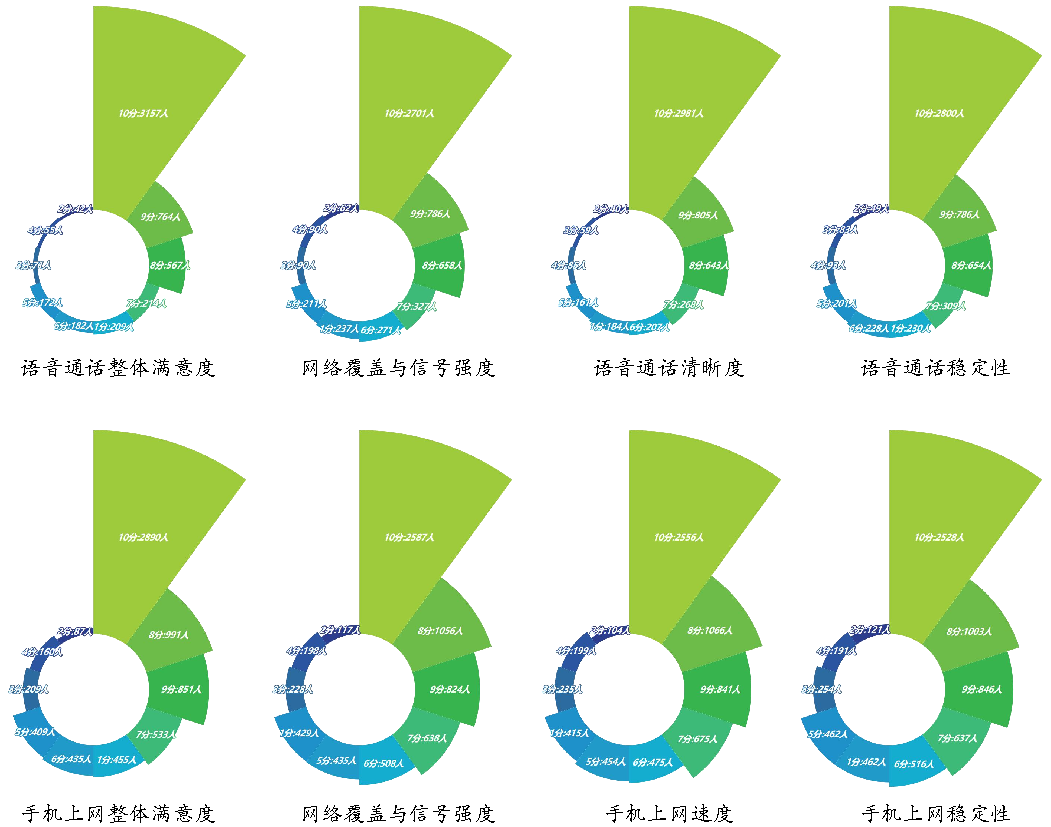
\includegraphics[scale=0.72]{南丁格尔玫瑰图F.pdf}}
		\caption{[附件1、附件2]各类评分人数南丁格尔玫瑰图}\label{fig:NightingaleRoseDiagramF}
	\end{figure}

	同时我们计算出各个最终模型(即八个Stacking集成学习后的模型)的准确率。然而观察到,各评分的分类不平衡,即某些评分的样本量要远远大于某些评分,见\textcolor{blue}{\cref{fig:NightingaleRoseDiagramF}}。因此,仅由准确率评估模型效果过于片面,且可能得到错误结论,因此我们还计算出各模型的平均绝对误差、均方误差,且准确率取五折交叉验证平均值,结果见\textcolor{blue}{\cref{tab:StackingResult}}。
	\begin{table}[htbp]
	\centering
	\caption{各评分预测模型效果}
	\setlength{\aboverulesep}{0pt}
	\setlength{\belowrulesep}{0pt}
	\scalebox{0.84}{
	  \begin{tabular}{cccc}
	  \toprule
	  \textbf{模型} & \textbf{五折交叉验证平均准确率} & \textbf{平均绝对误差} & \textbf{均方误差} \\
	  \midrule
	  模型一[预测语音业务,语音通话整体满意度] & 0.5773  & 1.2937  & 6.3877  \\
	  模型二[预测语音业务,网络覆盖与信号强度] & 0.4880  & 1.5387  & 7.3416  \\
	  模型三[预测语音业务,语音通话清晰度] & 0.5405  & 1.3527  & 6.4540  \\
	  模型四[预测语音业务,语音通话稳定性] & 0.5212  & 1.3913  & 6.3748  \\
	  模型五[预测上网业务,手机上网整体满意度] & 0.4359  & 1.7094  & 8.0684  \\
	  模型六[预测上网业务,网络覆盖与信号强度] & 0.3803  & 1.7650  & 7.7764  \\
	  模型七[预测上网业务,手机上网速度] & 0.3761  & 1.7208  & 7.3134  \\
	  模型八[预测上网业务,手机上网稳定性] & 0.3875  & 1.8276  & 8.0897  \\
	  \bottomrule
	  \end{tabular}}
	\label{tab:StackingResult}
	\end{table}
  
	我们将\textcolor{blue}{\cref{tab:RFXGBoost}}、\textcolor{blue}{\cref{tab:KNNSVM}}、\textcolor{blue}{\cref{tab:LightGBMLR}}与\textcolor{blue}{\cref{tab:StackingResult}}进行对比分析,可以发现,Stacking模型较其组成的模型各结果均有一定优化,且预测结果有良好的稳健性。Stacking学习其组成模型的优势,更大范围地高效利用数据集间隐藏的关系,具有良好的预测效果。


	为了更好地评估模型,对预测结果的合理性进行分析,我们绘制出各个模型的\textbf{混淆矩阵热力图}、\textbf{分类报告}、\textbf{ROC/AUC曲线}。这里由于篇幅原因,我们仅展示“预测语音业务-语音通话整体满意度”三幅模型效果可视化图形,其余模型的分析与其一致。对于其余模型的可视化图形,读者可在附录中查看。其余七个模型的混淆矩阵热力图见\textcolor{blue}{\cref{fig:SecondModelConfusionMatrix}}\textasciitilde\textcolor{blue}{\cref{fig:EighthModelConfusionMatrix}};分类报告见\textcolor{blue}{\cref{fig:SecondModelClassificationReport}}\textasciitilde\textcolor{blue}{\cref{fig:EighthModelClassificationReport}};ROC/AUC曲线见\textcolor{blue}{\cref{fig:SecondModelROCAUC}}\textasciitilde\textcolor{blue}{\cref{fig:EighthModelROCAUC}}。
	\begin{itemize}
		\item \textbf{混淆矩阵热力图}。该可视化图形的每一行表示样本标签的实际类别,在本题中表示用户评分的实际值\textcolor{blue}{\footnote{上文中提到我们对用户评分进行标签编码,从原来的$\left[1,10\right]$映射至新评分标签$\left[0,9\right]$,即在原评分基础上减$1$,而在混淆矩阵热力图及分类报告图示中我们将标签编码已映射回原评分,对于模型的ROC/AUC曲线,我们未映射回原评分。}},而每一行表示样本标签的预测类别,在本题中表示用户评分的预测值。因此该图示的主对角线数据之和即为模型预测准确的样本数。对于多分类模型,我们可以随机指定一类为正类,而其余就为对应的负类。这里我们需要引入四项值,分别为$TP$、$FN$、$FP$、$TN$,其中T为True,F为False,这两个字母表示预测值与实际值是否相同;P为Positive,N为Negative,这两个字母表示预测出的是属于正类(阳性)还是负类(阴性)。而混淆矩阵热力图即为这些值组成,该图示可以直观地观察到预测准确与错误的情况,以及模型对于每一类别的区分程度。模型一的混淆矩阵热力图见\textcolor{blue}{\cref{fig:FirstModelConfusionMatrix}}。
		\begin{figure}[H]
			\centerline{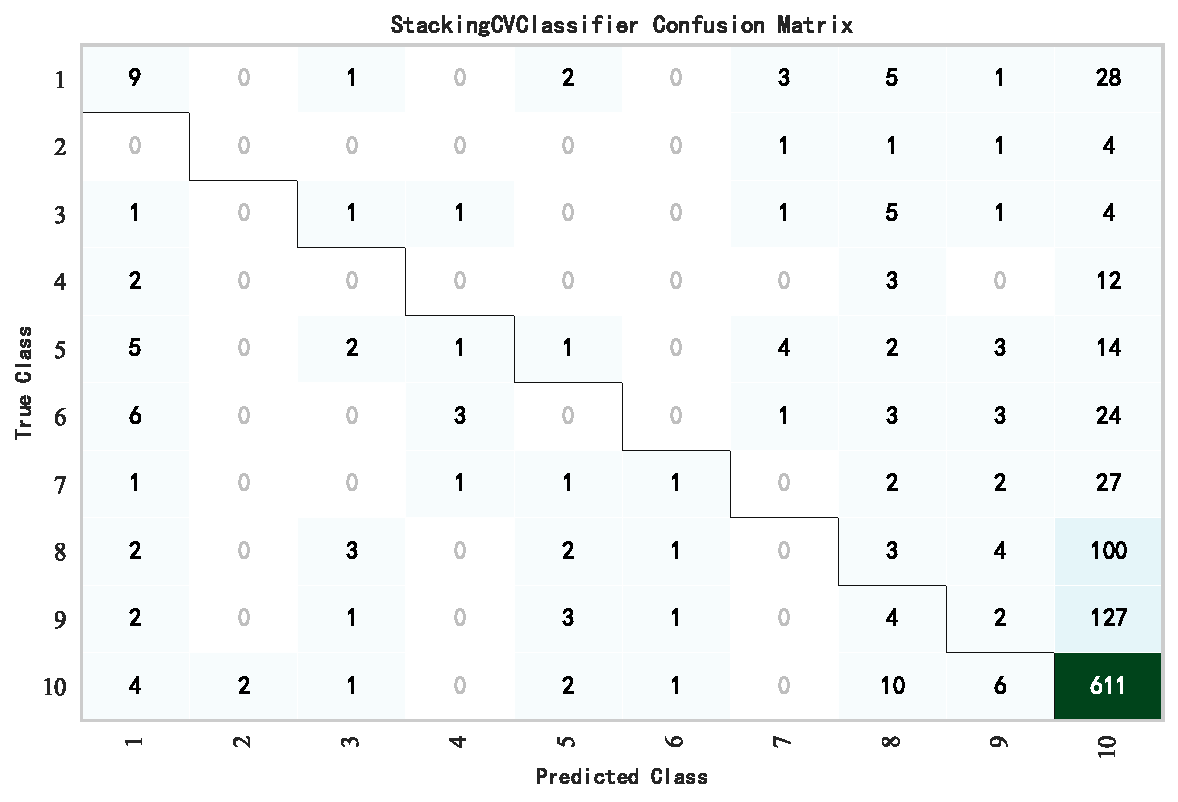
\includegraphics[scale=0.60]{[附件1]模型一混淆矩阵热力图.pdf}}
			\caption{模型一混淆矩阵热力图[语音业务-语音通话整体满意度]}\label{fig:FirstModelConfusionMatrix}
		\end{figure}

		观察该图,我们可以发现,该模型对于预测用户评分具有较好的效果,主对角线附近元素较多,说明模型预测正确的误差较小,预测得分与用户实际评分比较接近,可以较好预测用户评分。

		\item \textbf{分类报告}。分类报告图示可以直观得到模型各项参数,包括每一类别的精确率(Precision),召回率(Recall),F1分数值(F1-Score)。对于这三项值,其计算公式如下:
		\begin{itemize}
			\item {\heiti 精确率}
			\begin{equation}
				\mathrm{Precision} = \frac{TP}{TP+FP} \label{Precision}
			\end{equation}
			\item {\heiti 召回率}
			\begin{equation}
				\mathrm{Recall} = \frac{TP}{TP+FN} \label{Recall}
			\end{equation}
			\item {\heiti F1分数值} 
			\begin{equation}
				\mathrm{F}1 = \frac{2\times \mathrm{Precision}\times \mathrm{Recall}}{\mathrm{Precision}+\mathrm{Recall}}=\frac{TP}{TP+\frac{1}{2}\left(FP+FN\right)} \label{F1-Score}
			\end{equation}
		\end{itemize}
		根据上述\textcolor{blue}{\eqref{Precision}}、\textcolor{blue}{\eqref{Recall}}、\textcolor{blue}{\eqref{F1-Score}},我们可以计算出每一个模型对于每一类别的三项指标值,并绘制分类报告图,对于模型一的分类报告,见\textcolor{blue}{\cref{fig:FirstModelClassificationReport}}。此外我们还利用宏观(Macro)、微观(Micro)、权重(Weighted)三种方法计算模型的精确率、召回率以及F1分数值。宏观方法即取所有类别得出的值的平均值,不考虑样本的不平衡性;微观方法将所有样本视为整体;权重方法计算的是加权平均值。结果见\textcolor{blue}{\cref{tab:MacroMicroWeighted}}。
		\begin{figure}[htbp]
			\centerline{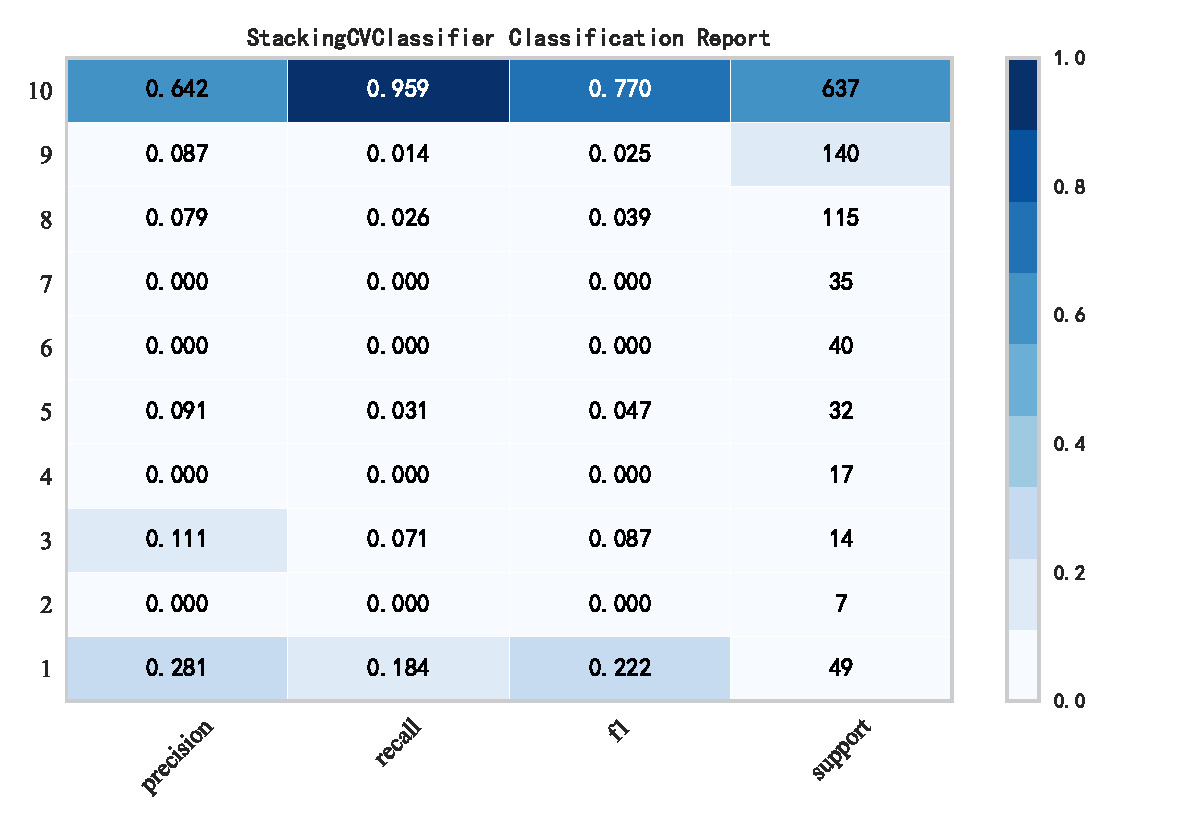
\includegraphics[scale=0.50]{[附件1]模型一分类报告.pdf}}
			\caption{模型一分类报告[语音业务-语音通话整体满意度]}\label{fig:FirstModelClassificationReport}
		\end{figure}

		\begin{table}[htbp]
			\centering
			\caption{模型一宏观、微观、权重计算准确率、召回率、F1分数值}
			\setlength{\aboverulesep}{0pt}
			\setlength{\belowrulesep}{0pt}
			\scalebox{0.88}{
			\begin{tabular}{cccc}
			\toprule
			\textbf{Method} & \textbf{Precision} & \textbf{Recall} & \textbf{F1-Score} \\
			\midrule
			Macro & 0.1291  & 0.1285  & 0.1190  \\
			Micro & 0.5773  & 0.5773  & 0.5773  \\
			Weighted & 0.4373  & 0.5855  & 0.4841  \\
			\bottomrule
			\end{tabular}}
			\label{tab:MacroMicroWeighted}
		\end{table}
		根据上述图表,我们可以发现,对于不平衡的样本数据,若仅仅计算模型的准确率,显然不能很好体现模型的效果,同时我们也应该根据实际业务需求,对Macro及Micro方法进行综合分析。在样本类别的数目分布不均衡时,Macro方法会同等对待每一种分类;而Micro方法较Macro方法更加趋向于客观结果的分析。此外,对于模型的精确率、召回率,我们可以根据定义发现,这两项值显然较大,模型效果较好。同时根据定义,我们可以发现模型的精确率、召回率在理想情况下是相差较小的,我们可以根据图表结果验证,符合预期效果。对于模型的F1分数值,其为精确率与召回率的调和平均数,因此当精确率与召回率均有较好表现时,F1分数值会有较优秀表现。我们也可对\textcolor{blue}{\eqref{F1-Score}}进行一定变换,可以得到
		\begin{equation}
			\mathrm{F}1=\frac{2}{\frac{1}{\mathrm{Precision}}+\frac{1}{\mathrm{Recall}}} \label{ReacllNew}
		\end{equation}
		根据该式,我们可以得出上述结论。
		\item \textbf{ROC/AUC曲线}。在分析特征曲线及曲线下面积(Receiver Operating Characteristic/Area Under the Curve, ROC/AUC)图之前,我们需要了解模型的相关参数,定义如下:
		\begin{itemize}
			\item {\heiti 灵敏度}\textbf{(Sensitivity)}。灵敏度又被称为真阳性率,即$TP$率,定义为:
			\begin{equation}
				\mathrm{Sensitivity}=TPR=\frac{TP}{TP+FN} \label{Sensitivity}
			\end{equation}
			\item {\heiti 特异性}\textbf{(Specificity)}。特异性又被称为真阴性率,即$TN$率,定义为:
			\begin{equation}
				\mathrm{Specificity}=TNR=\frac{TN}{TN+FP} \label{Specificity}
			\end{equation}
			\item \textbf{1-Specificity}。称为假阳性率(False Positive Rate, $FPR$),定义为:
			\begin{equation}
				FPR=1-\mathrm{Specificity}=\frac{FP}{FP+TN} \label{FPR}
			\end{equation}
			\item \textbf{1-Sensitivity}。称为假阴性率(False Negative Rate, $FNR$),定义为:
			\begin{equation}
				FNR=1-\mathrm{Sensitivity}=\frac{FN}{FN+TP} \label{FNR}
			\end{equation}
		\end{itemize}
		$FPR$和$FNR$均对数据分布的变化不敏感\textcolor{blue}{\cite{procauc}},因此这两个指标可以用于在不平衡的数据上建立的模型效果的评价。
		
		对于ROC/AUC曲线,其以每一类别的$1-\mathrm{Specificity}$即$FPR$为横坐标,以$\mathrm{Sensitivity}$即$TPR$为纵坐标,其可体现出模型的灵敏度与特异性之间的关系与差异。因此,该图的理想点位于左上角,即$FPR=0$且$TPR=1$,换言之,当曲线越靠近左上角,模型效果就越优。从而,我们可以得到另一项指标,即曲线下面积(Area Under the Curve, AUC),由上述分析可知,AUC值越高,模型的整体效果也就越优。对于模型一的ROC/AUC曲线,见\textcolor{blue}{\cref{fig:FirstModelROCAUC}}。
		\begin{figure}[H]
			\centerline{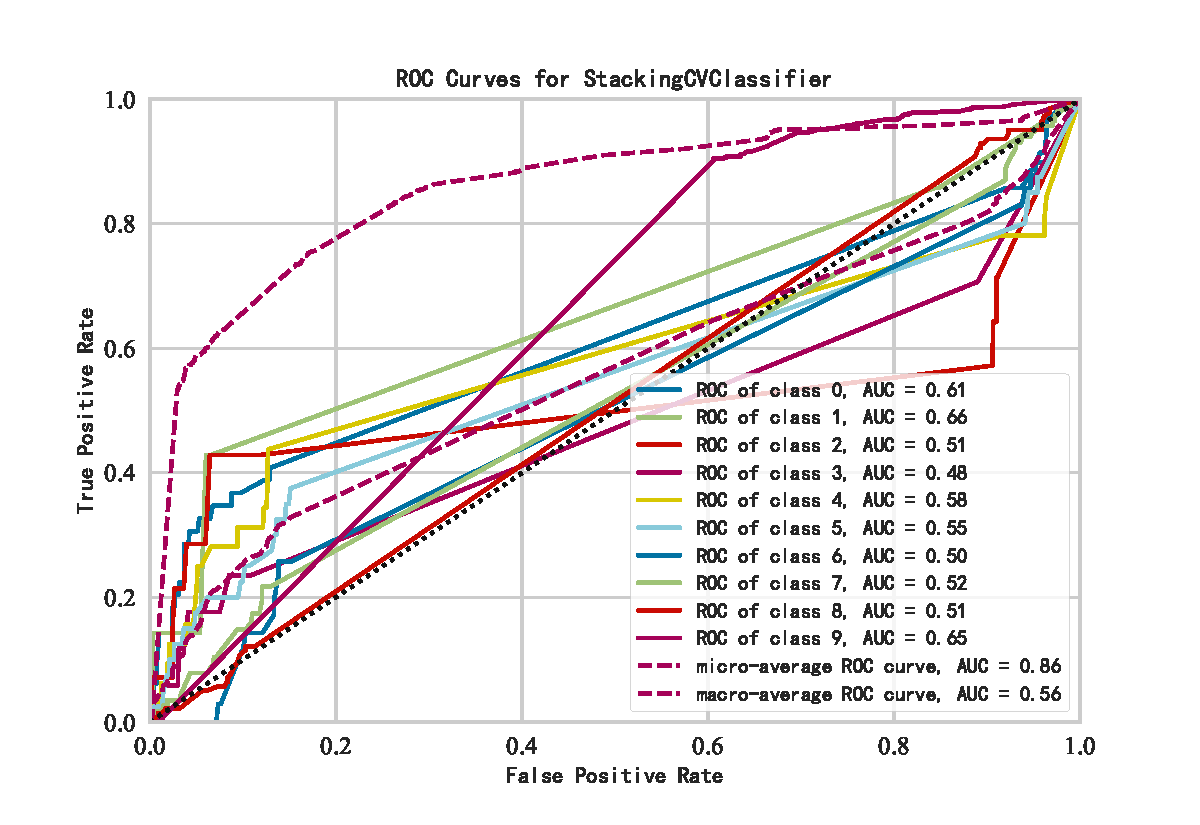
\includegraphics[scale=0.60]{[附件1]模型一ROCAUC.pdf}}
			\caption{模型一ROC/AUC曲线[语音业务-语音通话整体满意度]}\label{fig:FirstModelROCAUC}
		\end{figure}
		根据上图结果,我们可以发现,模型一预测用户对于“语音业务-语音通话整体满意度”的评分结果中,除对于类别$3$(即实际评分为$4$分)的$\mathrm{AUC}<0.50$之外,其余的$\mathrm{AUC}\geqslant0.50$,即以$y=x$为分界线。同时,我们可以发现“macro-average ROC curve”指标,其是通过Macro方法求得,在上文中我们提到,该数据样本的标签分类是严重不平衡的,该方法能够平等对待每一项分类,在此方法下,我们可以对于小样本类别的准确率有一定把握,其曲线下面积$\mathrm{AUC}=0.56$,位于分界线左上,预测效果良好;而对于“micro-average ROC curve”指标,其$\mathrm{AUC}=0.86$,这指的是利用Micro方法求得曲线,曲线下面积为0.86,曲线下面积较大,且曲线有向左上角最优点靠近的趋势,可以说明模型整体能力较优。
	\end{itemize}
	
	此外,为观察预测出的评分分布是否大体与已知评分数据集评分分布大致一致,我们再次绘制南丁格尔玫瑰图,见\textcolor{blue}{\cref{fig:NightingaleRoseDiagramP}}。观察该图及\textcolor{blue}{\cref{fig:NightingaleRoseDiagramF}},我们可以发现预测出的评分分布与已知评分数据集评分分布大体一致,符合数据的一般性及内在规律。
	\begin{figure}[H]
		\centerline{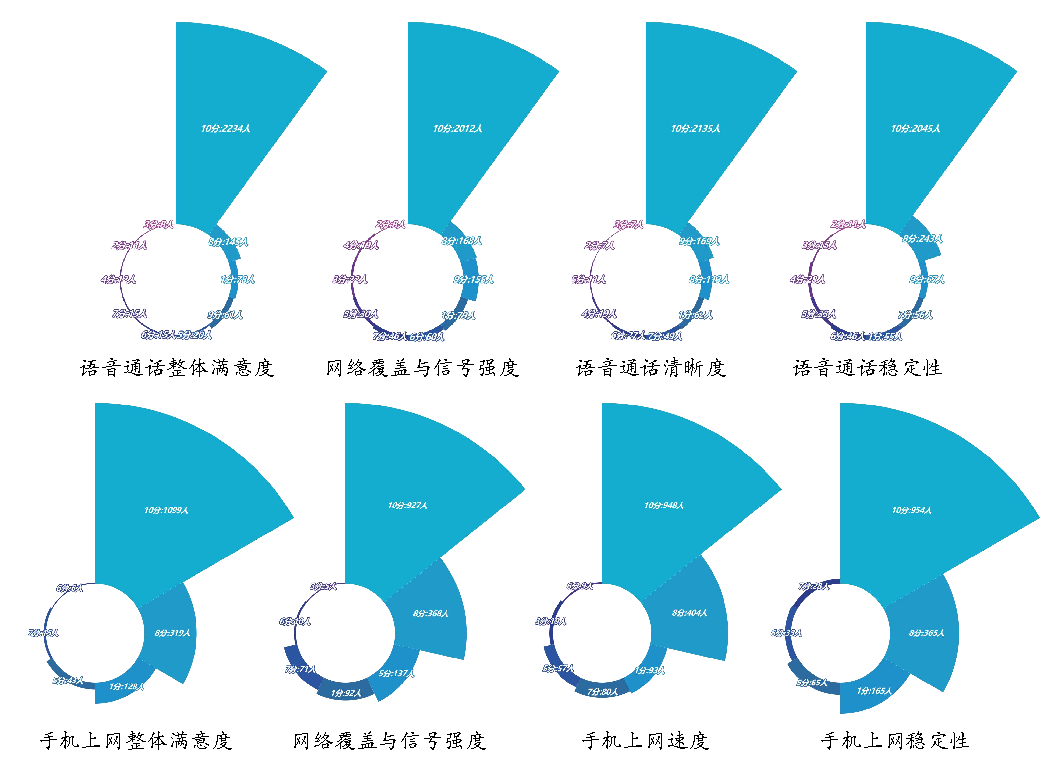
\includegraphics[scale=0.70]{南丁格尔玫瑰图P.pdf}}
		\caption{[附件3、附件4]各类评分人数南丁格尔玫瑰图}\label{fig:NightingaleRoseDiagramP}
	\end{figure}

	对于模型一[预测语音业务,语音通话整体满意度],根据\textcolor{blue}{\cref{tab:StackingResult}},我们可以发现,其五折交叉验证平均准确率为$57.73\%$,平均绝对误差为$1.2937$,均方误差为$6.3877$,即平均每位用户评分预测误差控制在$1$分左右,易得均方根误差为$\sqrt{6.3877}\approx2.5274$,可以发现,预测值与准确值误差程度在可接受范围内,预测效果较好。而此外,我们知道,对于用户评分,其属于主观性评分,而该评分难以准确量化,给模型带来一定复杂性,即在相近的分数处,较难以区分。此外,对于部分用户,可能存在未详细阅读问卷,导致乱评、错评现象,这一类属于明显异常值,显然,该预测模型可以在一定程度上识别出异常值,且效果良好。同时,我们绘制模型的混淆矩阵热力图、分类报告、ROC/AUC曲线,从上述分析中,我们有理由认为模型的预测效果较好,但同时也存在一定缺陷,如对小类样本的预测有一定难以区分的现象,而若我们要更多地分析研究小样本用户的情况,这会带来一定的局限性,我们也将在后文提及改进措施。
	\section{模型的评价与推广}
	\subsection{模型的评价}
	\begin{itemize}
		\item \textbf{模型的优点}:
			\begin{enumerate}
				\item 对数据进行综合处理,层次清晰,模型具有一定解释性;
				\item 数据标准化,避免量纲不一造成的偏向学习影响的情况;
				\item 特征筛选,减少不重要性因素占比,减少数据维度,提升模型学习效率,一定程度上避免数据噪声,适当降低模型复杂度,使模型高效化,防止过拟合;
				\item 特征构造,由原数据构造出新数据特征,适当增多数据维度,防止欠拟合;
				\item 综合熵权法、灰色关联度分析及随机森林量化影响程度,避免局部最优;
				\item 对各模型进行参数调优,尽可能提高模型的多方面能力;
				\item 加入正则化方法,一定程度上也可防止过拟合;
				\item 交叉验证,更好地利用数据集,减少数据浪费,提高模型的泛化能力,验证模型的稳健性,防止过拟合情况的发生;
				\item 模型设置任意随机种子,在保证划分训练集及测试集的一般性、随机性的同时,确保可重复性的结果,方便后续处理;
				\item 通过主成分分析及随机森林进行特征选择,保证客观性;
				\item 多模型Stacking集成学习,更好地利用已有数据,多方面学习数据中内在联系,结合多个模型优良方面,避免陷入局部最优,对数据有更好的把控能力,提升模型的泛化能力、提高预测准确率、提高模型稳健性、鲁棒性,同时减小预测误差,且对异常值有一定识别能力。
			\end{enumerate}
		\item \textbf{模型的缺点}:
			\begin{enumerate}
				\item 模型对于小样本分类的识别能力较差,难以对这些用户进行深入分析;
				\item 模型对于预测主观性评分,难以提供完全一致的评分结果;
				\item Stacking在构造时,有一定复杂度,对基模型的要求较高;
				\item 对于部分评分,特征构造出的因素有一定局限性;
				\item 用户评分为主观性结果,本文大多模型选用客观性较强的模型进行解决,对数据利用有一定失真。
			\end{enumerate}
		\newpage
		\item \textbf{模型的改进}:
			\begin{enumerate}
				\item 在收集数据时,问卷设计需要更加合理化,多方面考虑其余未考虑到的影响因素对用户评分的影响;
				\item 在允许条件下获得更多训练样本;
				\item 对各模型可以选用非完全一致的特征,提升各模型的独特性,有目的地进行选择,减少学习的数据维度,加快模型收敛速度,使得模型学习高效化,结果准确化;
				\item 适当增加或减少数据维度,建立复杂度适中的模型;
				\item 对不平衡的多分类,可以采用“下采样”或“上采样”方法,使得分类平衡,但需要更多的数据集;
				\item 可适当增加基模型个数,并提高对基模型的筛选要求;
				\item 对主观性评分,可以建立主客观相结合的模型,从而优化模型各项指标。
			\end{enumerate}
	\end{itemize}
	\subsection{模型的推广}
	机器学习可利用现有的数据集进行有目的的训练,在此基础上预测分类标签下人为难以确定的结果,极大方便了当今对复杂数据的处理;多种机器学习相互结合,利用Stacking集成学习的方法,可以有效提高模型各方面能力,减少判断错误的情况。针对小部分样本的学习,需要更容易区分类别的特征进行学习,以及利用特征工程等方法进行解决。对于机器学习模型,我们可以作出其可视化图像,观察到模型的各项指标不易发现的问题,如欠拟合、过拟合等情况,我们可以依据模型效果评估可视化来对模型进行一定的调优。本文是以移动用户对业务的评分为基础,我们运用了多种机器学习的模型,再结合Stacking进行集成学习,可以发现模型的效果较优,对主观性评分模型有较好把控能力。利用该模型,可以根据用户对某些影响因素的情况,预测用户对于这项业务的满意程度,再结合相关描述性信息,有的放矢地解决用户遇到的问题,提升客户的满意程度,提升产品的服务质量,从而为业务创造更多价值。该模型在一定程度上虽有一定欠缺,但不仅仅可用于该领域的评分,也可用于其余领域,如用户对于某一产品的评价预测,根据用户评价,改善产品质量,提升经济效益,实现双赢。

	\newpage
	\phantomsection
	\addcontentsline{toc}{section}{\textbf{参考文献}}
	\begin{spacing}{1.08}
	\begin{thebibliography}{99}
	\bibitem{pstandard}CSDN.【数据预处理】sklearn实现数据预处理(归一化、标准化)[EB/OL].
	
	\url{https://blog.csdn.net/weixin_44109827/article/details/124786873}.

	\bibitem{ppearson1}肖杨,李亚,王海瑞,常梦容.基于皮尔逊相关系数的滚动轴承混合域特征选择方法[J].化工自动化及仪表,2022,49(03):308-315.DOI:10.20030/j.cnki.1000-3932.202203009.
	
	\bibitem{ppearson2}王殿武,赵云斌,尚丽英,王凤刚,张震.皮尔逊相关系数算法在B油田优选化学防砂措施井的应用[J].精细与专用化学品,2022,30(07):26-28.DOI:10.19482/j.cn11-3237.2022.07.07.

	\bibitem{pewm1}姚文宇,李杰,李岩峰,高娜,王涛. 基于熵权法的呼吸机质量综合评价研究[C]//.中国医学装备大会暨2022医学装备展览会论文汇编(下册).[出版者不详],2022:162-167.DOI:10.26914/c.cnkihy.2022.042155.

	\bibitem{pewm2}谢赤,钟赞.熵权法在银行经营绩效综合评价中的应用[J].中国软科学,2002(09):109-111+108.

	\bibitem{pgrey1}张广海,董跃蕾.青岛市旅游业影响因素灰色关联度分析及其发展路径[J].德州学院学报,2022,38(04):54-58.

	\bibitem{prf}饶雷,冉军,陶建权,胡号朋,吴沁,熊圣新.基于随机森林的海上风电机组发电机轴承异常状态监测方法[J].船舶工程,2022,44(S2):27-31.DOI:10.13788/j.cnki.cbgc.2022.S2.06.

	\bibitem{pxgboost1}陈振宇,刘金波,李晨,季晓慧,李大鹏,黄运豪,狄方春,高兴宇,徐立中.基于LSTM与XGBoost组合模型的超短期电力负荷预测[J].电网技术,2020,44(02):614-620.DOI:10.13335/j.1000-3673.pst.2019.1566.

	\bibitem{pxgboost2}杨贵军,徐雪,赵富强.基于XGBoost算法的用户评分预测模型及应用[J].数据分析与知识发现,2019,3(01):118-126.

	\bibitem{pxgboost3}Tianqi Chen and Carlos Guestrin. 2016. XGBoost: A Scalable Tree Boosting System. In Proceedings of the 22nd ACM SIGKDD International Conference on Knowledge Discovery and Data Mining (KDD '16). Association for Computing Machinery, New York, NY, USA, 785–794. \url{https://doi.org/10.1145/2939672.2939785}.

	\bibitem{ppca}傅湘,纪昌明.区域水资源承载能力综合评价——主成分分析法的应用[J].长江流域资源与环境,1999(02):168-173.

	\bibitem{pknn}张著英,黄玉龙,王翰虎.一个高效的KNN分类算法[J].计算机科学,2008(03):170-172.

	\bibitem{psvm}汪海燕,黎建辉,杨风雷.支持向量机理论及算法研究综述[J].计算机应用研究,2014,31(05):1281-1286.

	\bibitem{plightgbm}马晓君,沙靖岚,牛雪琪.基于LightGBM算法的P2P项目信用评级模型的设计及应用[J].数量经济技术经济研究,2018,35(05):144-160.DOI:10.13653/j.cnki.jqte.20180503.001.

	\bibitem{plr}唐敏,张宇浩,邓国强.高效的非交互式隐私保护逻辑回归模型[J/OL].计算机工程:1-11[2023-01-04].DOI:10.19678/j.issn.1000-3428.0065549.

	\bibitem{pstacking}史佳琪,张建华.基于多模型融合Stacking集成学习方式的负荷预测方法[J].中国电机工程学报,2019,39(14):4032-4042.DOI:10.13334/j.0258-8013.pcsee.181510.


	\bibitem{procauc}A.Tharwat, Applied Computing and Informatics (2018). \url{https://doi.org/10.1016/j.aci.2018.08.003}.

	\end{thebibliography}
	\end{spacing}
	\newpage

	\phantomsection
	\addcontentsline{toc}{section}{\textbf{附\hspace{2pc}录}}

	% \appendix
	% \ctexset{section={format={\zihao{-4}\heiti\raggedright}}}
	\begin{center}
		\heiti\zihao{4} 附\hspace{2pc}录
	\end{center}

% \phantomsection
% \addcontentsline{toc}{subsection}{[A]图示}
% 	% \section*{[A]图表}
	\noindent{\heiti [A]图表}
	\begin{figure}[H]
		\centerline{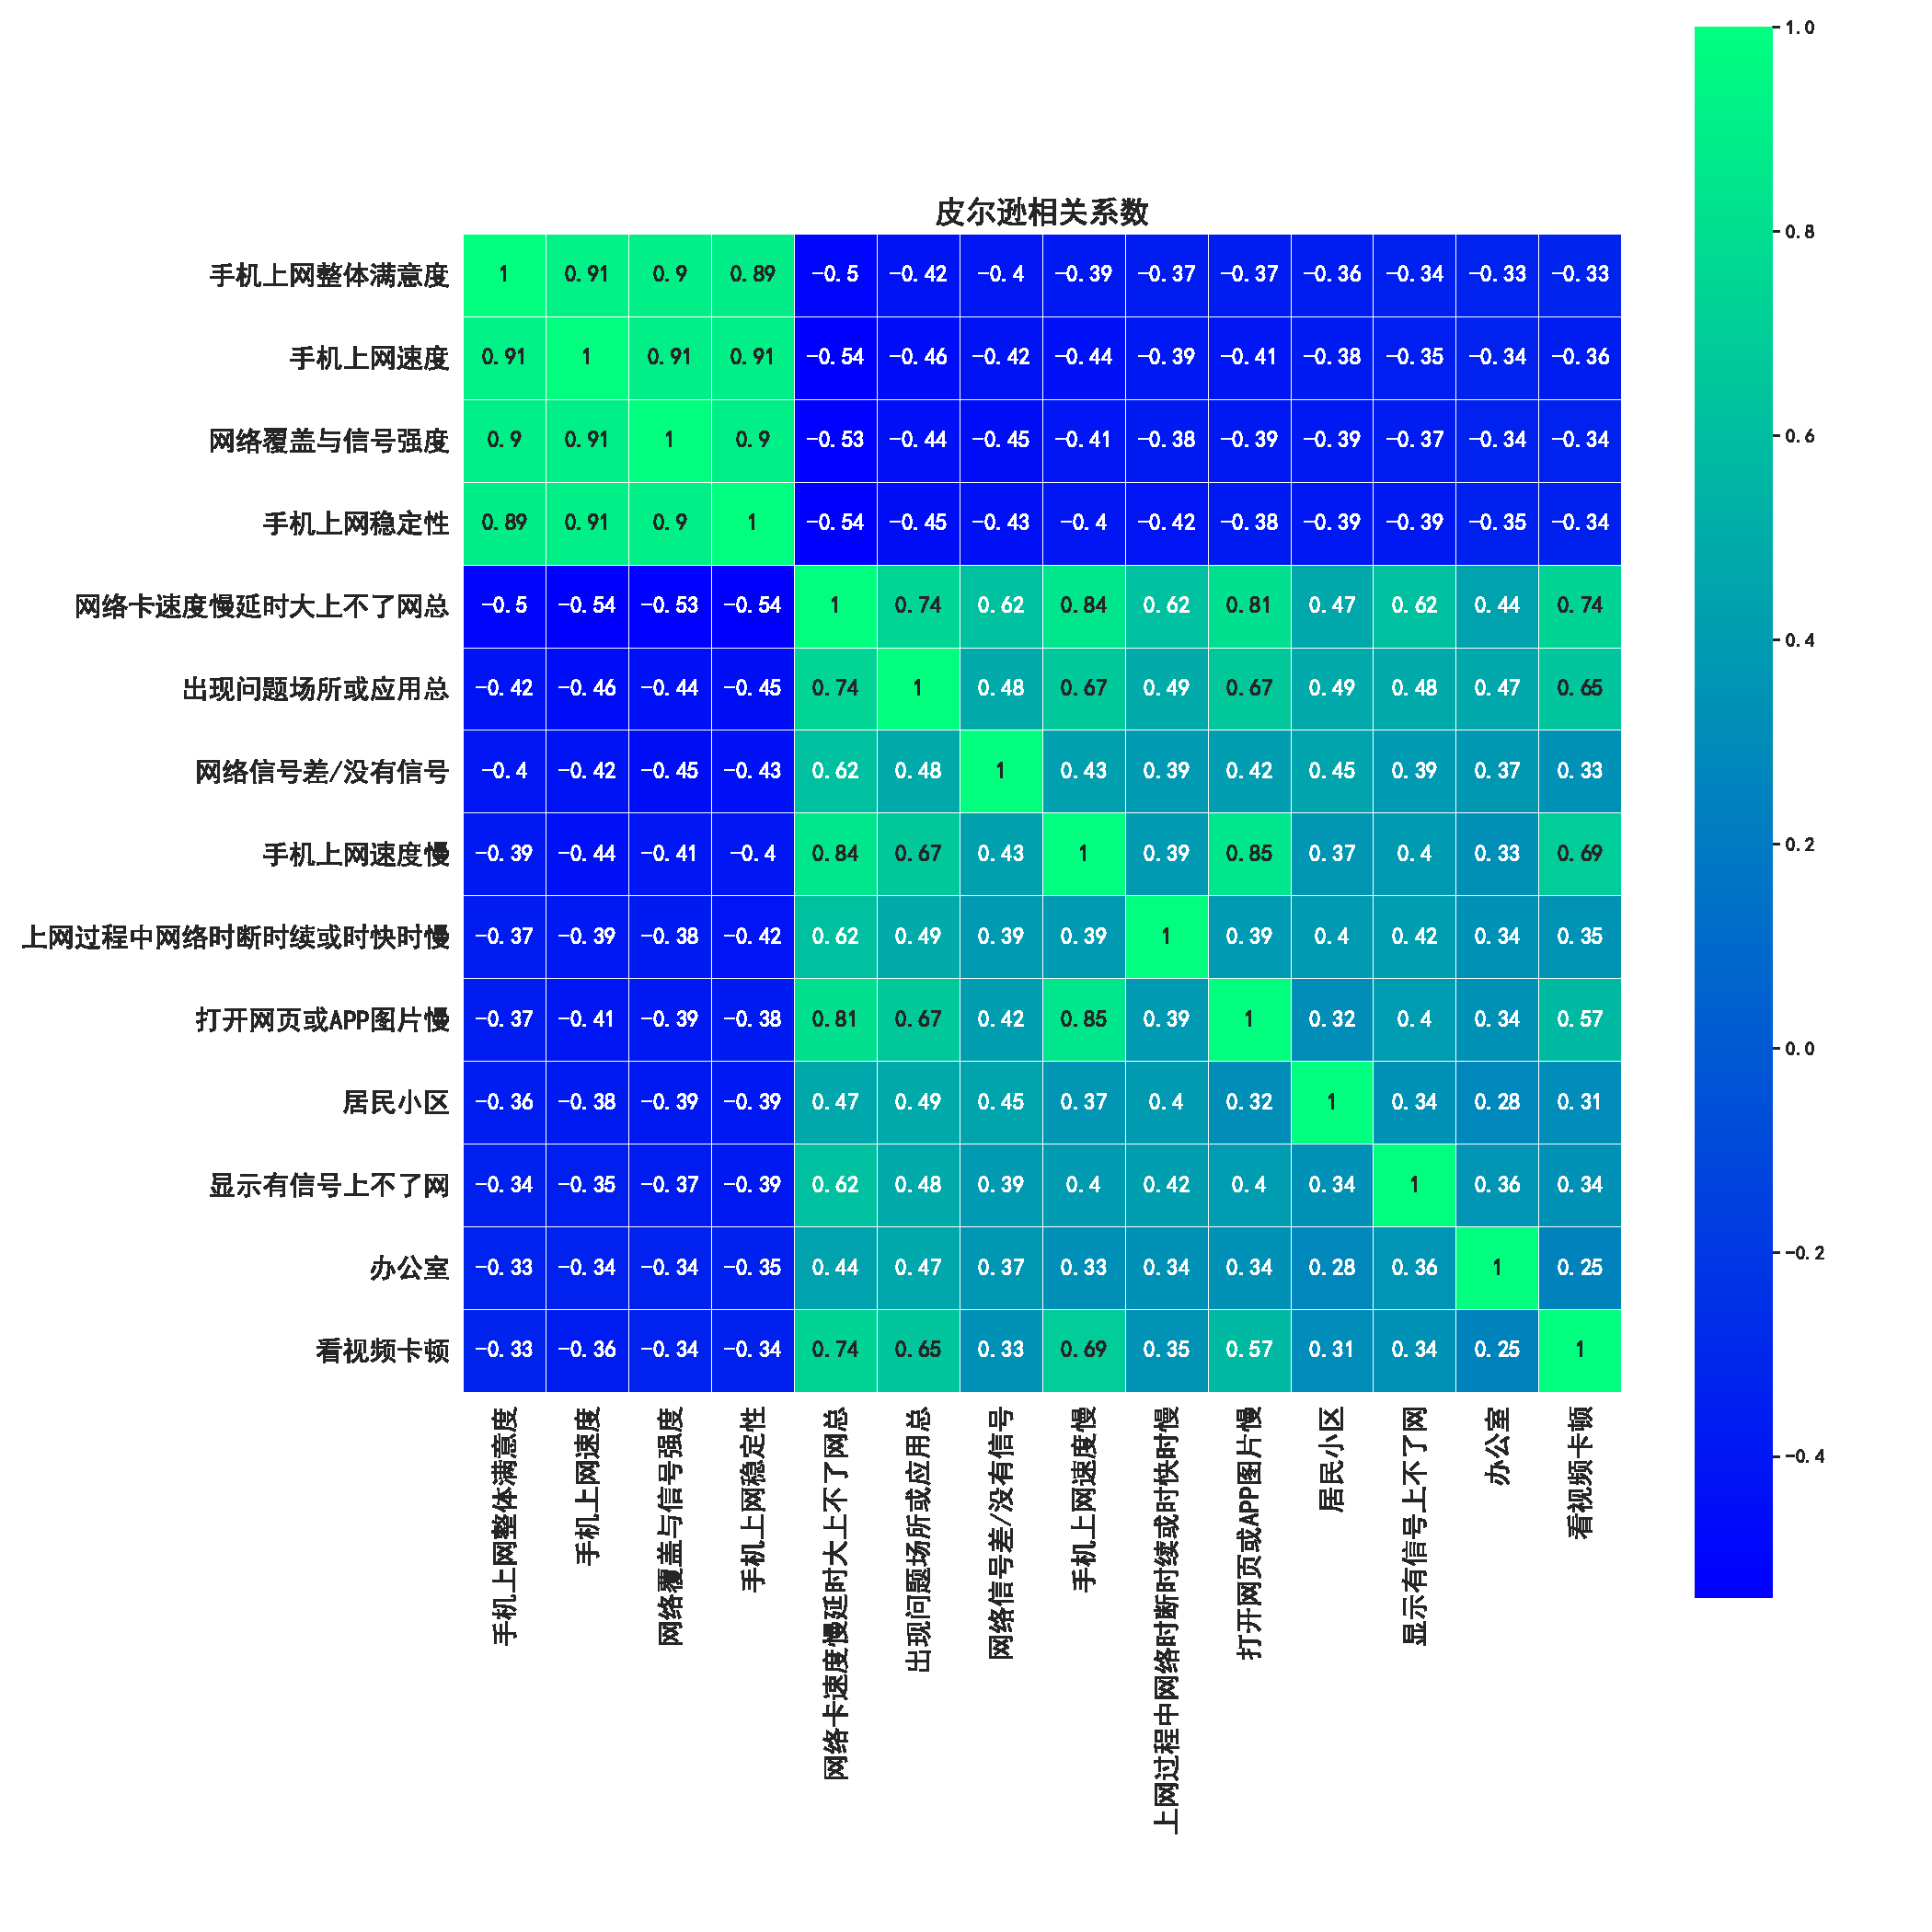
\includegraphics[scale=0.4]{[附件2]皮尔逊相关系数(14个).pdf}}
		\caption{上网业务评分与其影响因素皮尔逊相关系数热力图}\label{fig:a2perason}
	\end{figure}
	\begin{figure}[H]
		\centerline{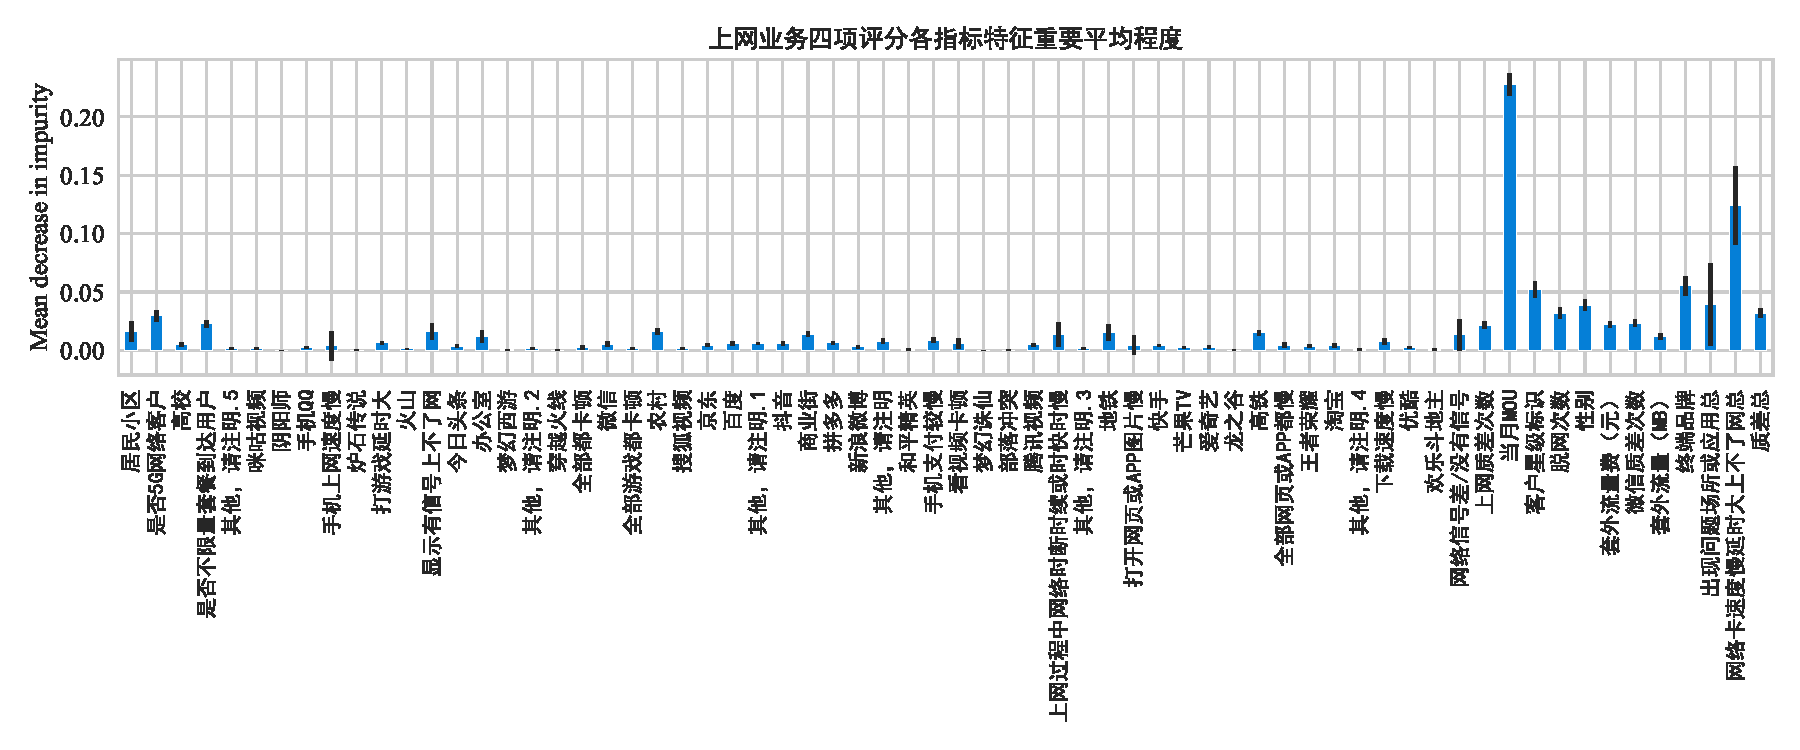
\includegraphics[scale=0.52]{[附件2]上网业务四项评分各指标特征重要平均程度.pdf}}
		\caption{上网业务四项评分各指标特征重要平均程度}\label{fig:a2allRF}
		\end{figure}
	\begin{figure}[H]
		\centerline{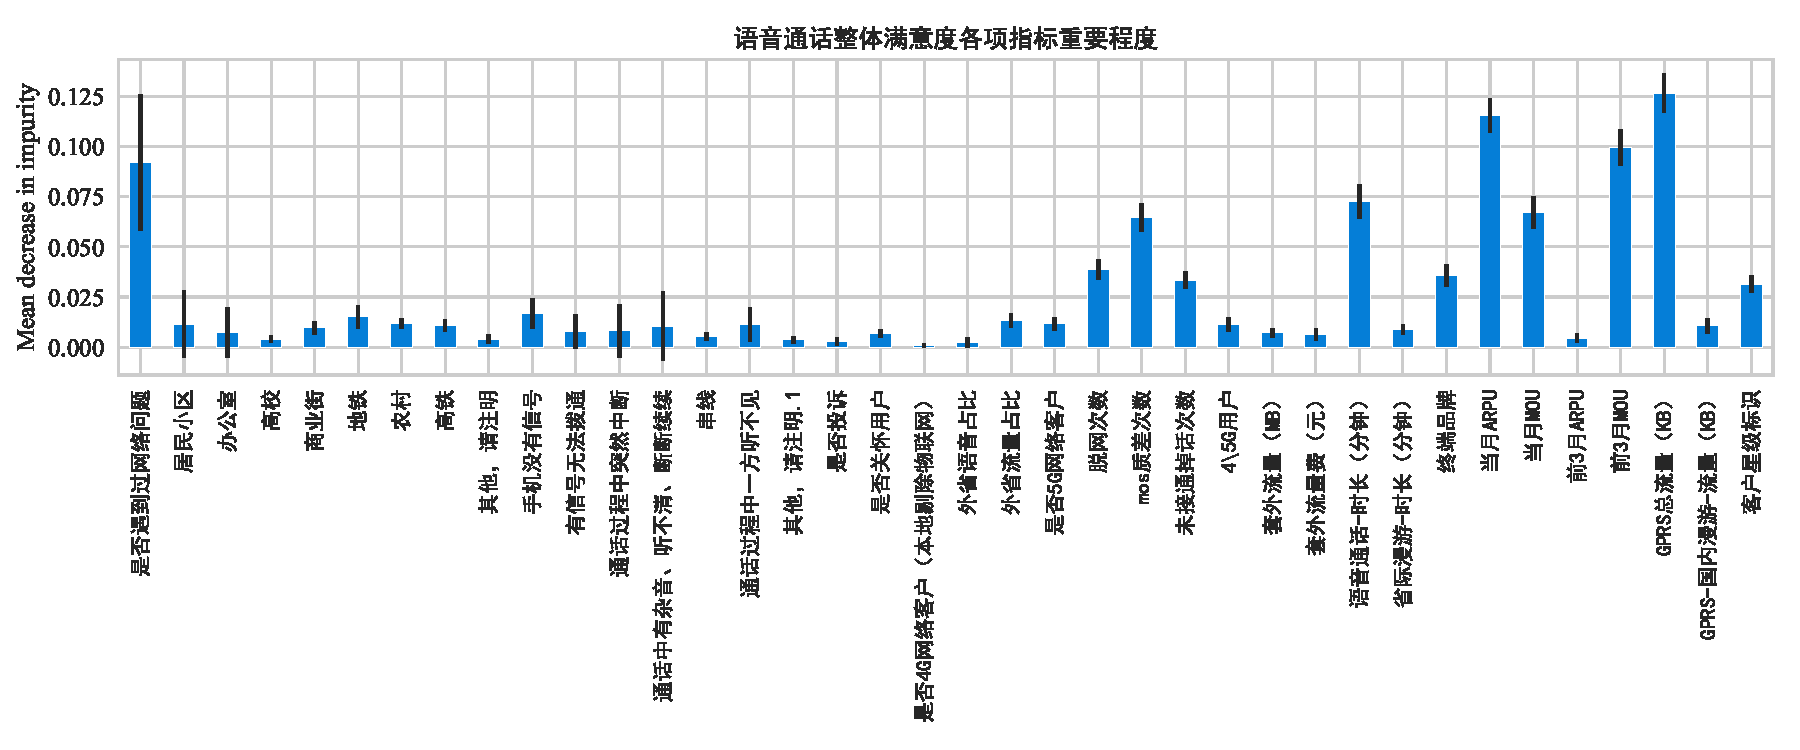
\includegraphics[scale=0.5]{[附件1]语音通话整体满意度各项指标重要程度.pdf}}
		\caption{语音业务-语音通话整体满意度各项指标重要程度}\label{fig:a1FirstRF}
	\end{figure}
	\begin{figure}[H]
		\centerline{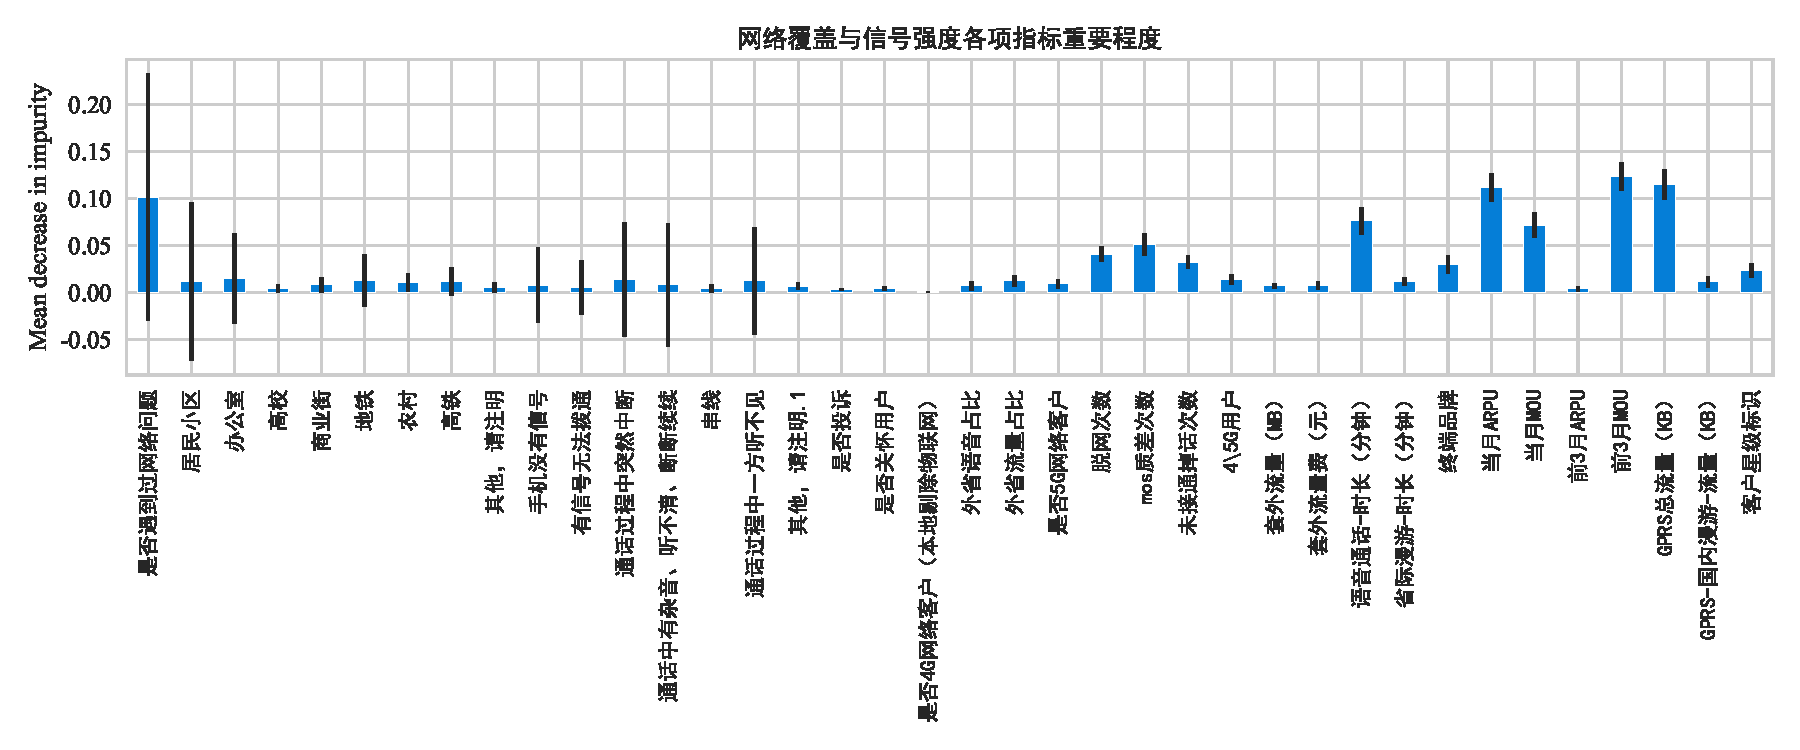
\includegraphics[scale=0.5]{[附件1]网络覆盖与信号强度各项指标重要程度.pdf}}
		\caption{语音业务-网络覆盖与信号强度各项指标重要程度}\label{fig:a1SecondRF}
	\end{figure}
	\begin{figure}[H]
		\centerline{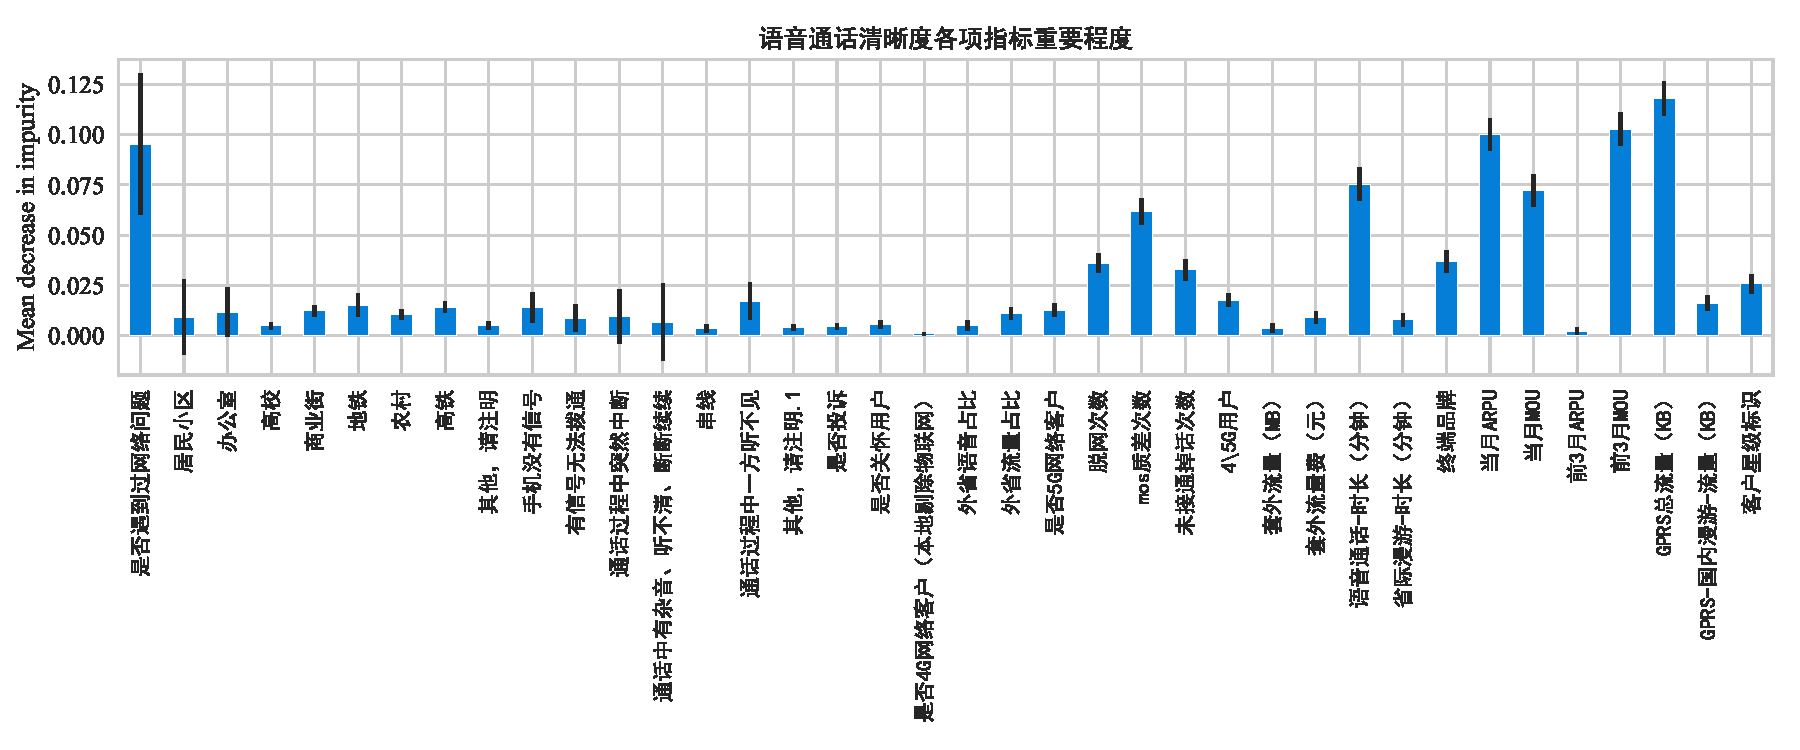
\includegraphics[scale=0.5]{[附件1]语音通话清晰度各项指标重要程度.pdf}}
		\caption{语音业务-语音通话清晰度各项指标重要程度}\label{fig:a1ThirdRF}
	\end{figure}
	\begin{figure}[H]
		\centerline{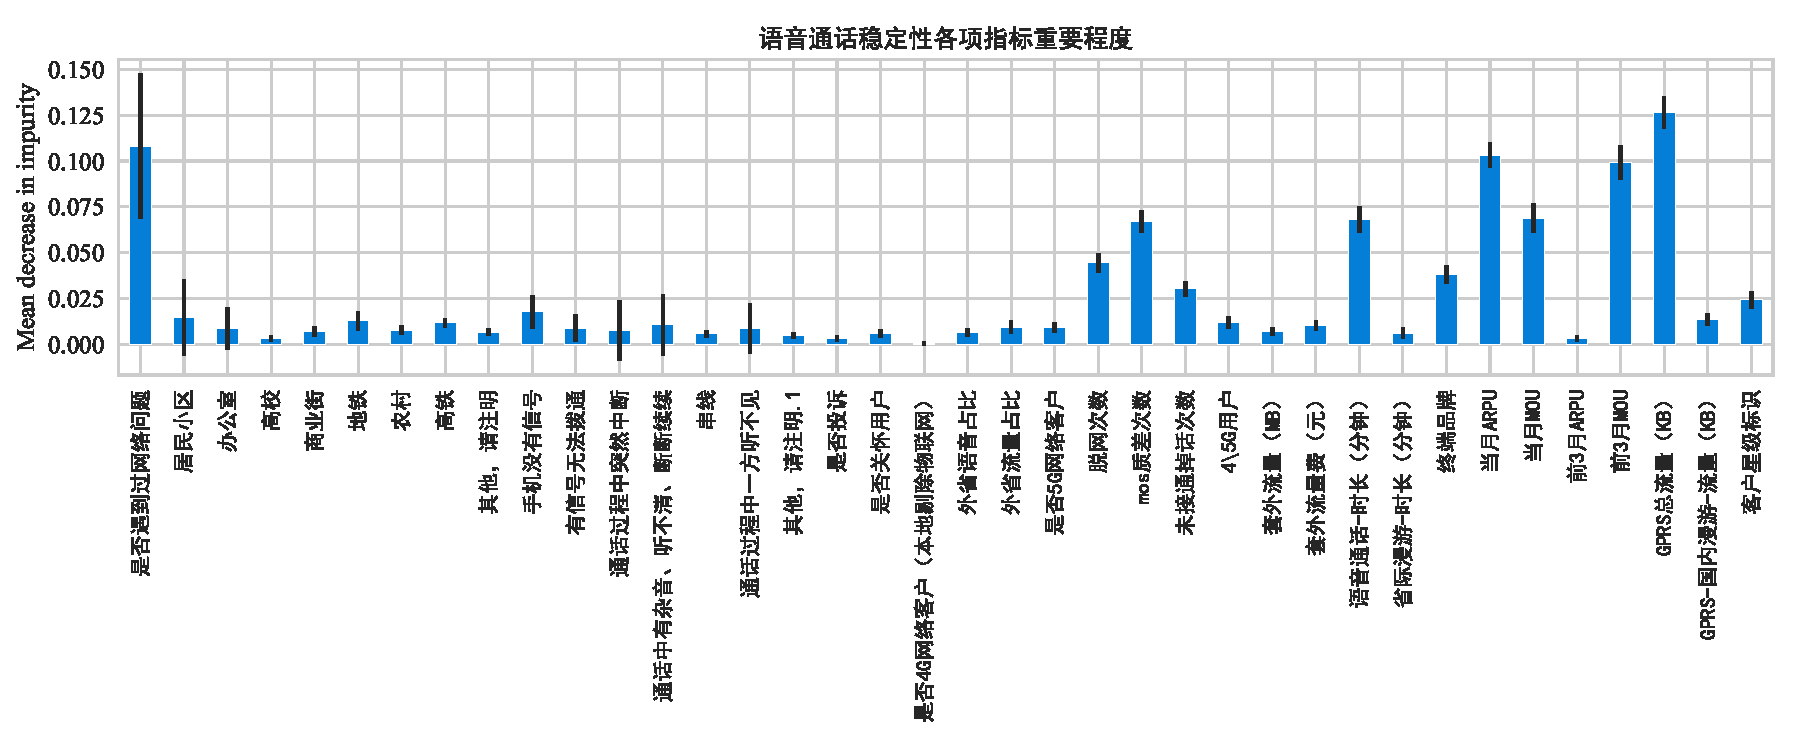
\includegraphics[scale=0.5]{[附件1]语音通话稳定性各项指标重要程度.pdf}}
		\caption{语音业务-语音通话稳定性各项指标重要程度}\label{fig:a1FourthRF}
	\end{figure}

	\begin{figure}[H]
		\centering
		\begin{minipage}{0.49\linewidth}
			\centering
			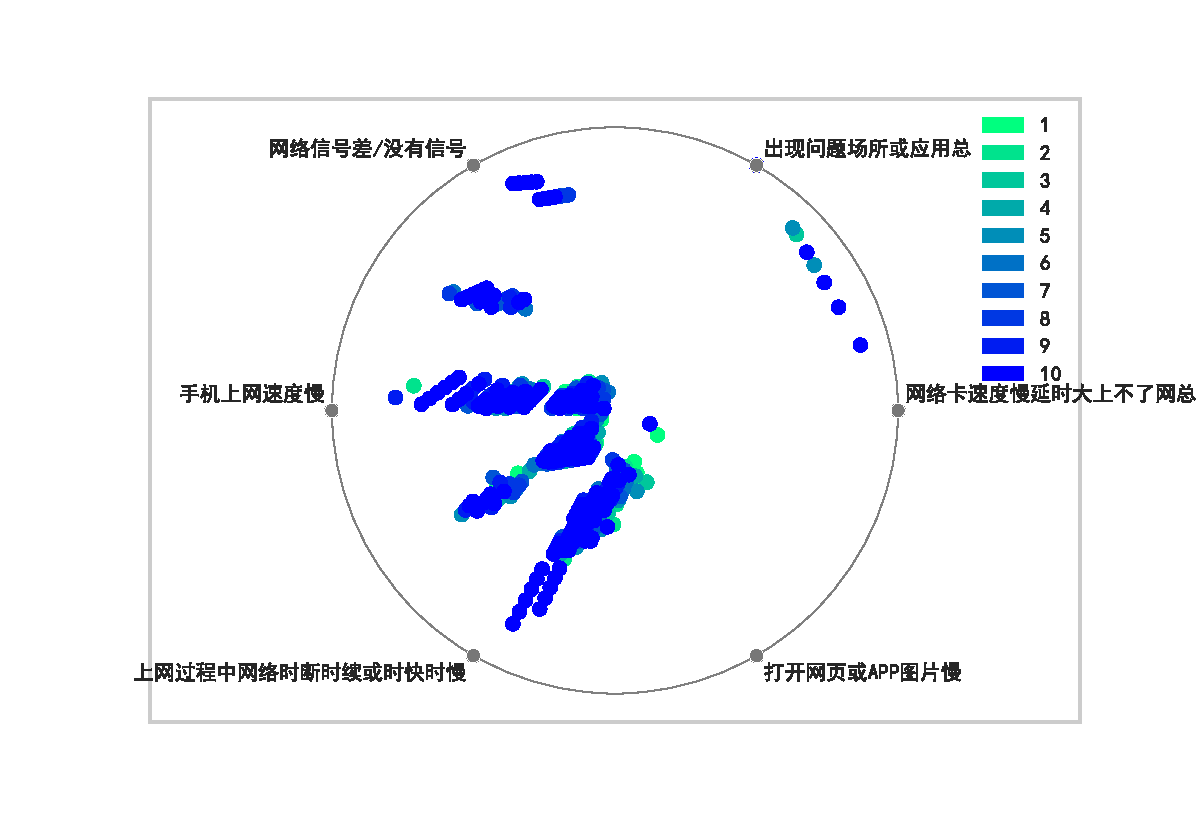
\includegraphics[width=0.9\linewidth]{[附件2]手机上网整体满意度RidViz.pdf}
			\caption{手机上网整体满意度RidViz}
			\label{fig:a2FirstRid}
		\end{minipage}
		\begin{minipage}{0.49\linewidth}
			\centering
			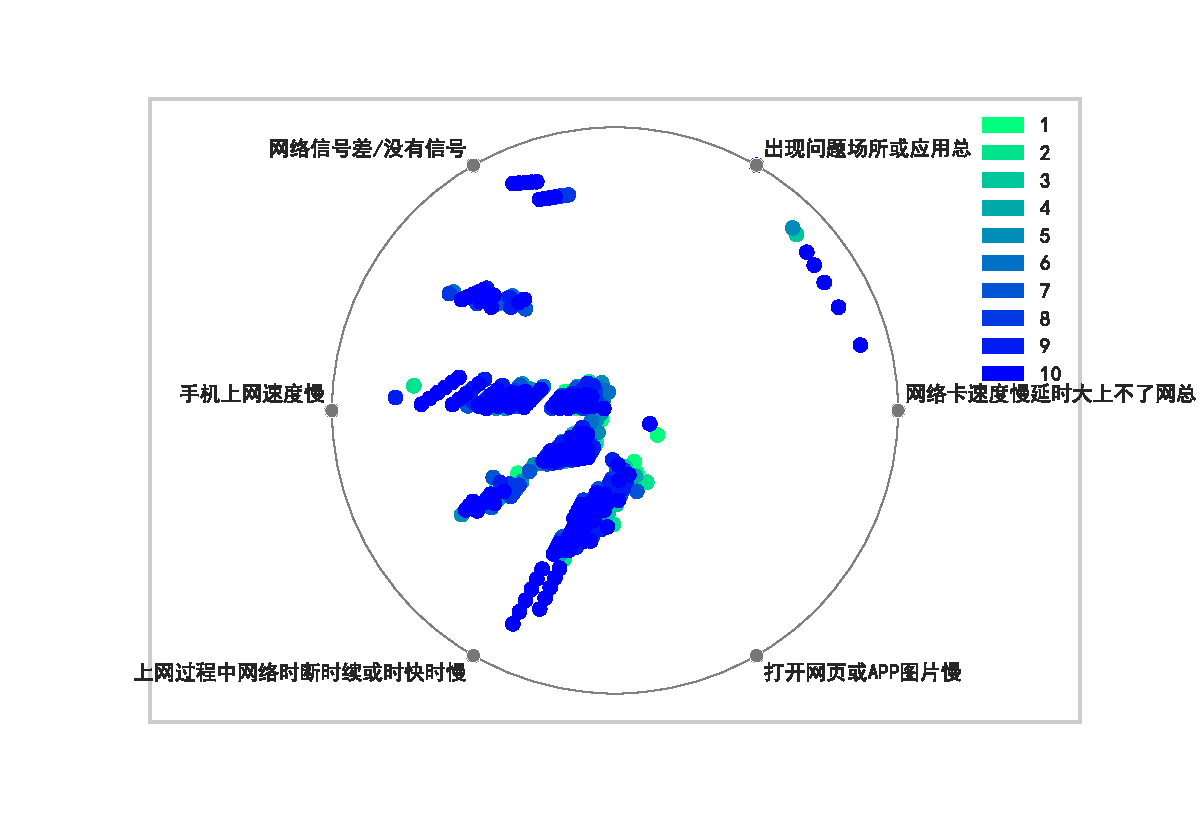
\includegraphics[width=0.9\linewidth]{[附件2]网络覆盖与信号强度RidViz.pdf}
			\caption{网络覆盖与信号强度与指标RidViz}
			\label{fig:a2SecondRid}
		\end{minipage}
		
		\begin{minipage}{0.49\linewidth}
			\centering
			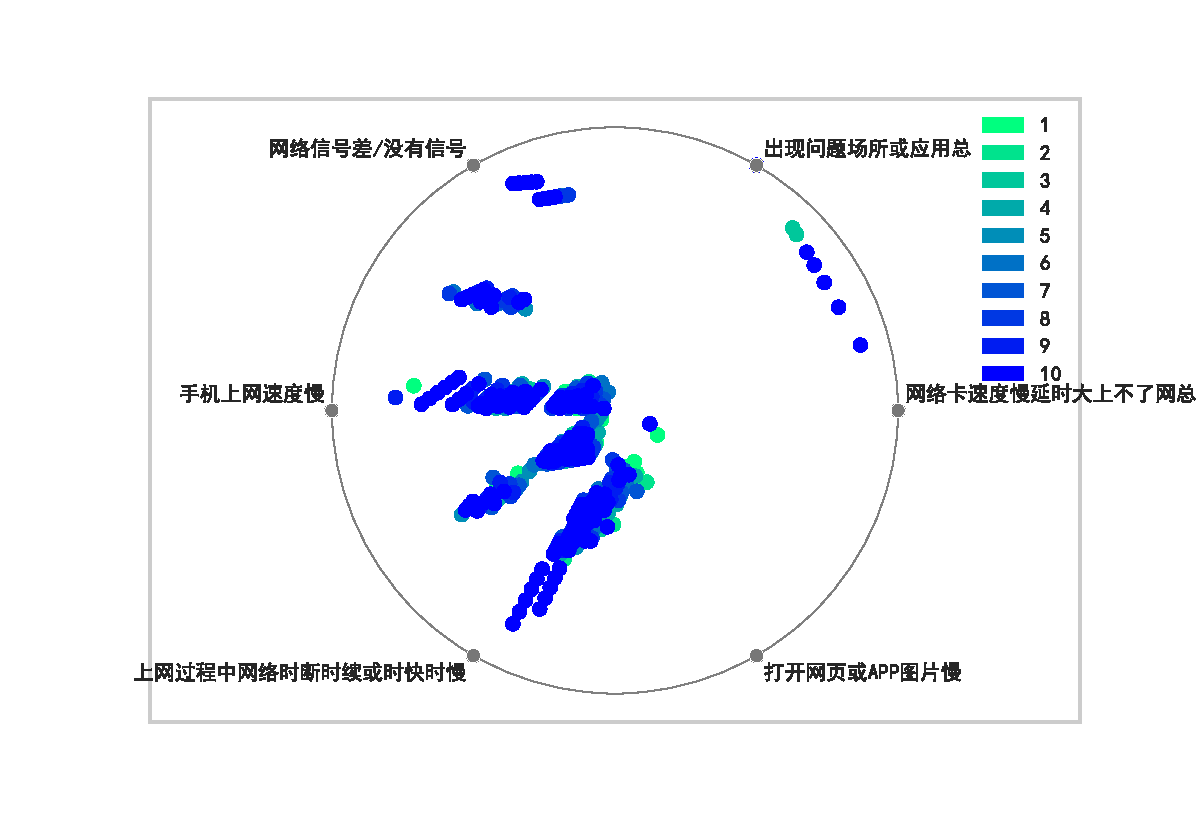
\includegraphics[width=0.9\linewidth]{[附件2]手机上网速度RidViz.pdf}
			\caption{手机上网速度RidViz}
			\label{fig:a2ThirdRid}
		\end{minipage}
		\begin{minipage}{0.49\linewidth}
			\centering
			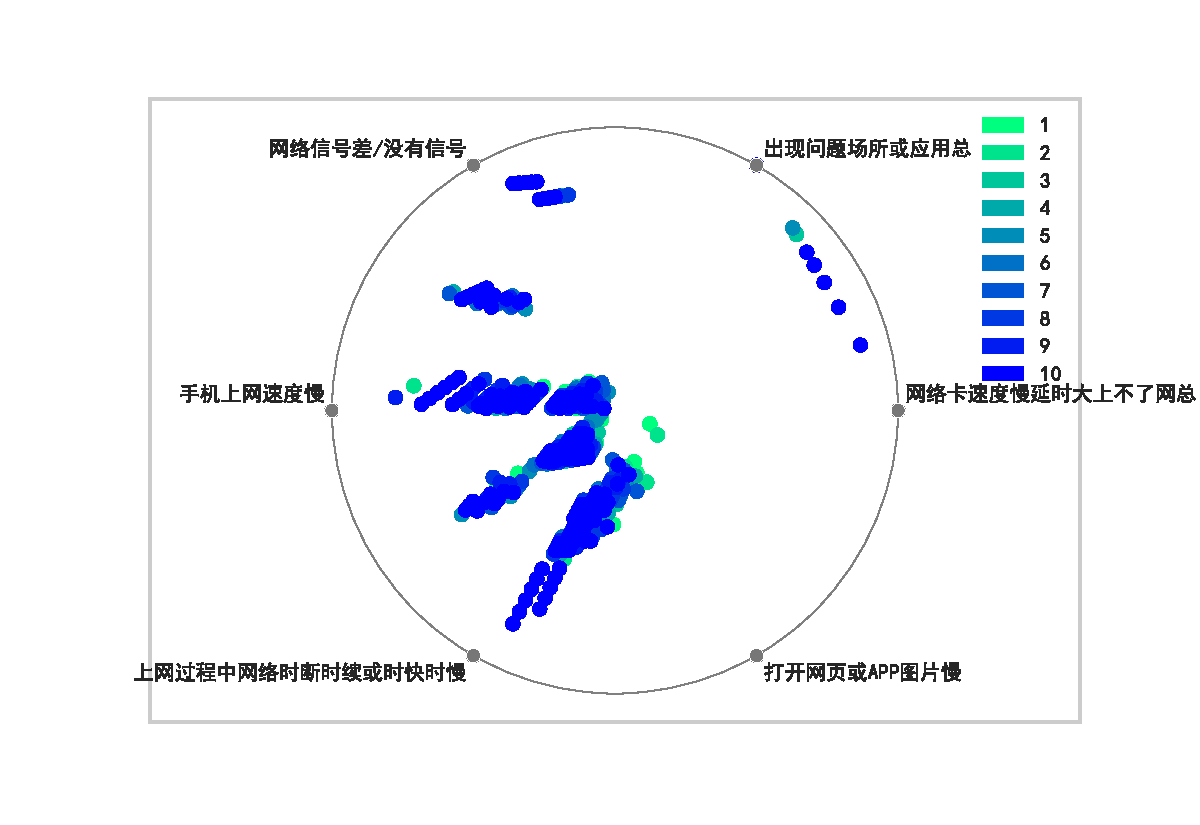
\includegraphics[width=0.9\linewidth]{[附件2]手机上网稳定性RidViz.pdf}
			\caption{手机上网稳定性RidViz}
			\label{fig:a2FourthRid}
		\end{minipage}
	\end{figure}

	\begin{figure}[H]
		\centerline{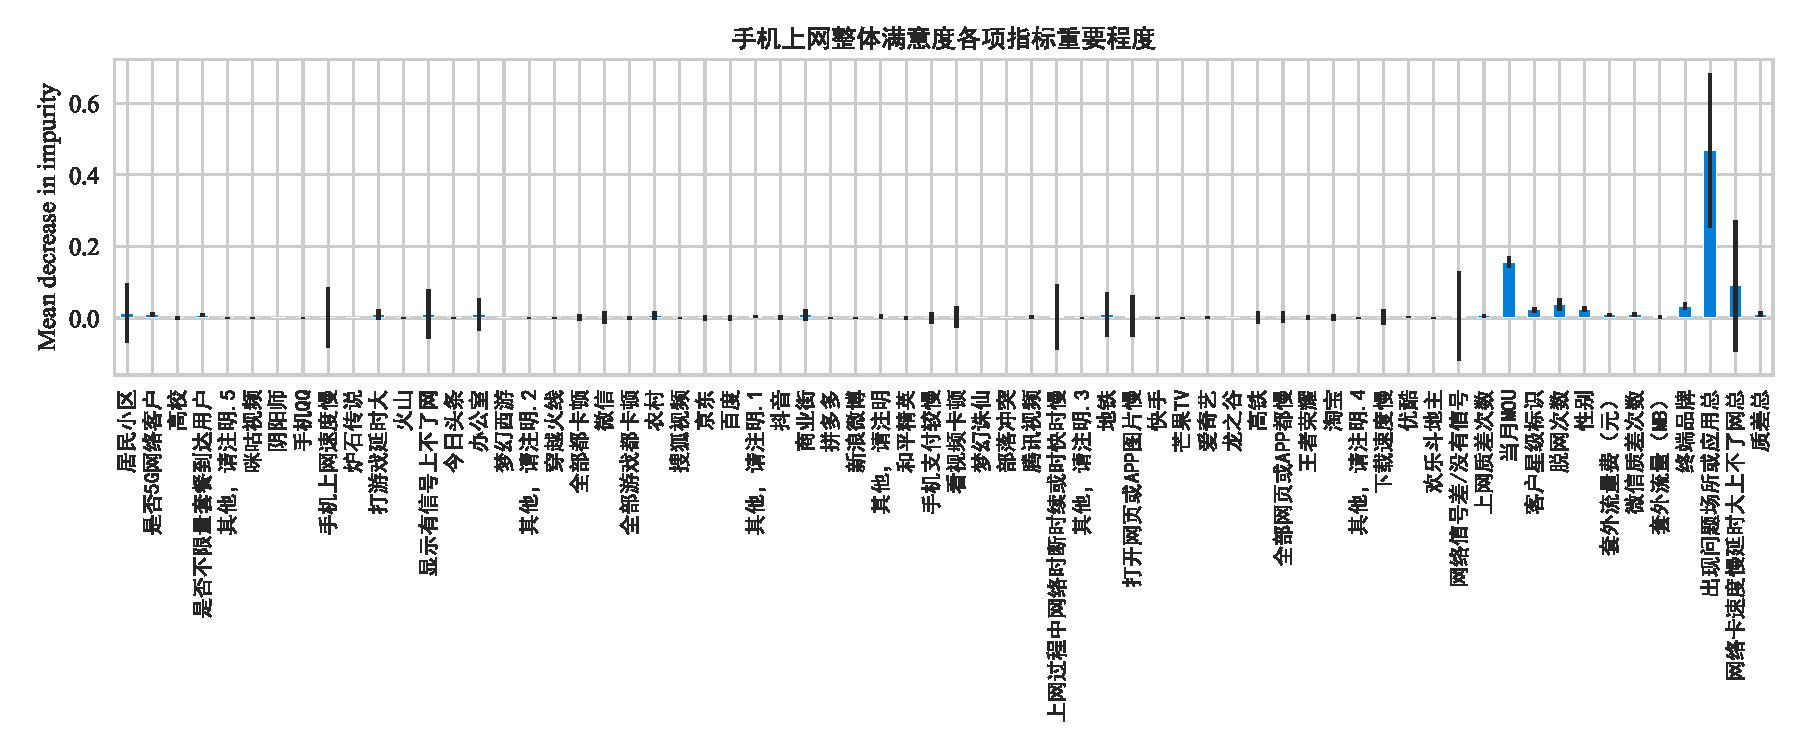
\includegraphics[scale=0.5]{[附件2]手机上网整体满意度各项指标重要程度.pdf}}
		\caption{上网业务-手机上网整体满意度各项指标重要程度}\label{fig:a2FirstRF}
	\end{figure}
	\begin{figure}[H]
		\centerline{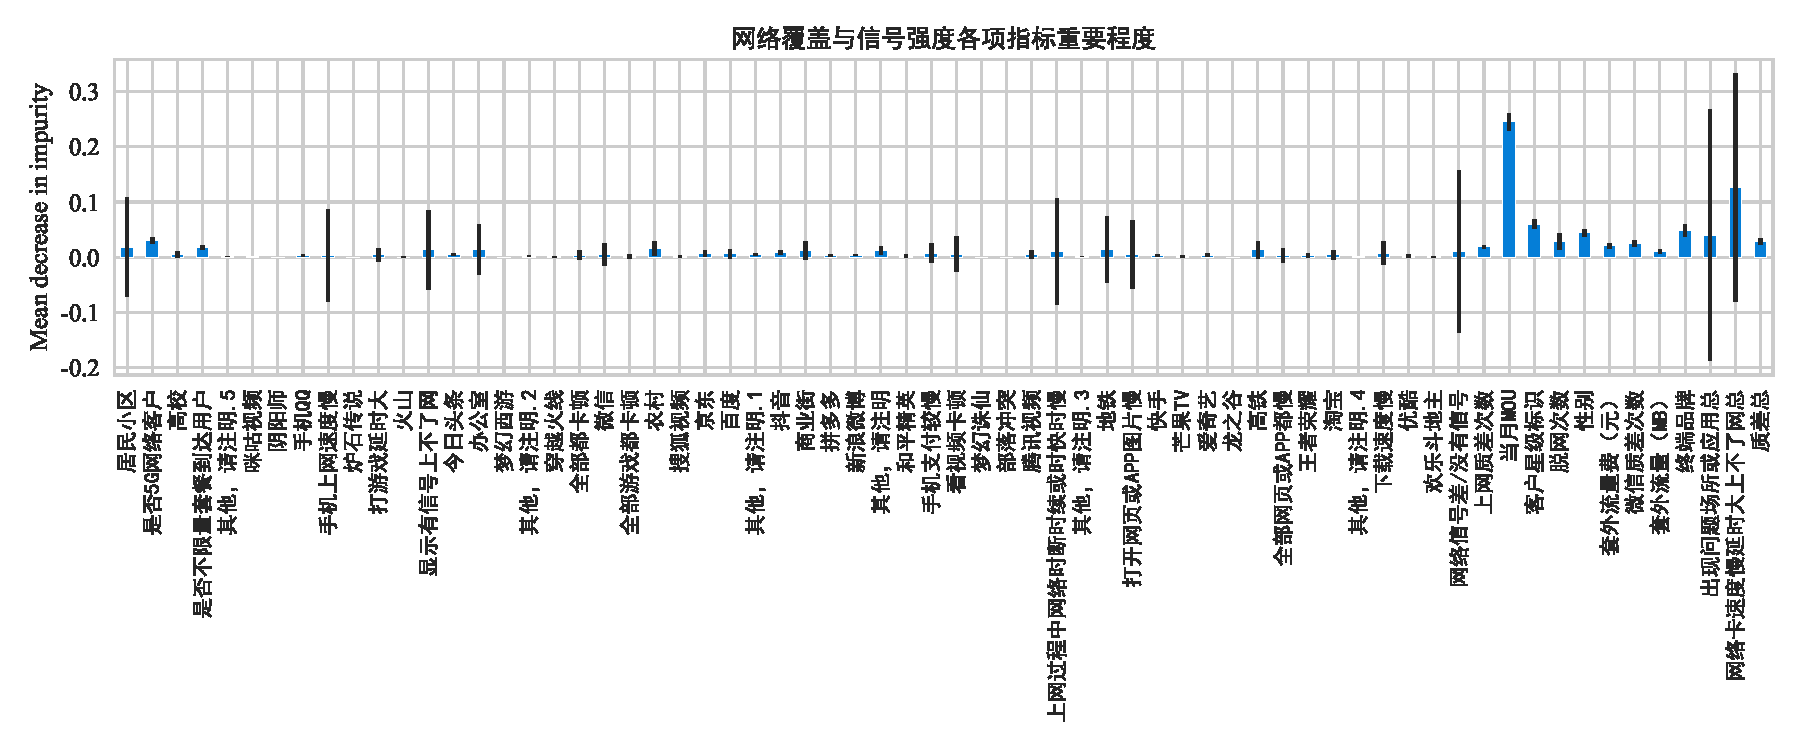
\includegraphics[scale=0.5]{[附件2]网络覆盖与信号强度各项指标重要程度.pdf}}
		\caption{上网业务-网络覆盖与信号强度各项指标重要程度}\label{fig:a2SecondRF}
	\end{figure}
	\begin{figure}[H]
		\centerline{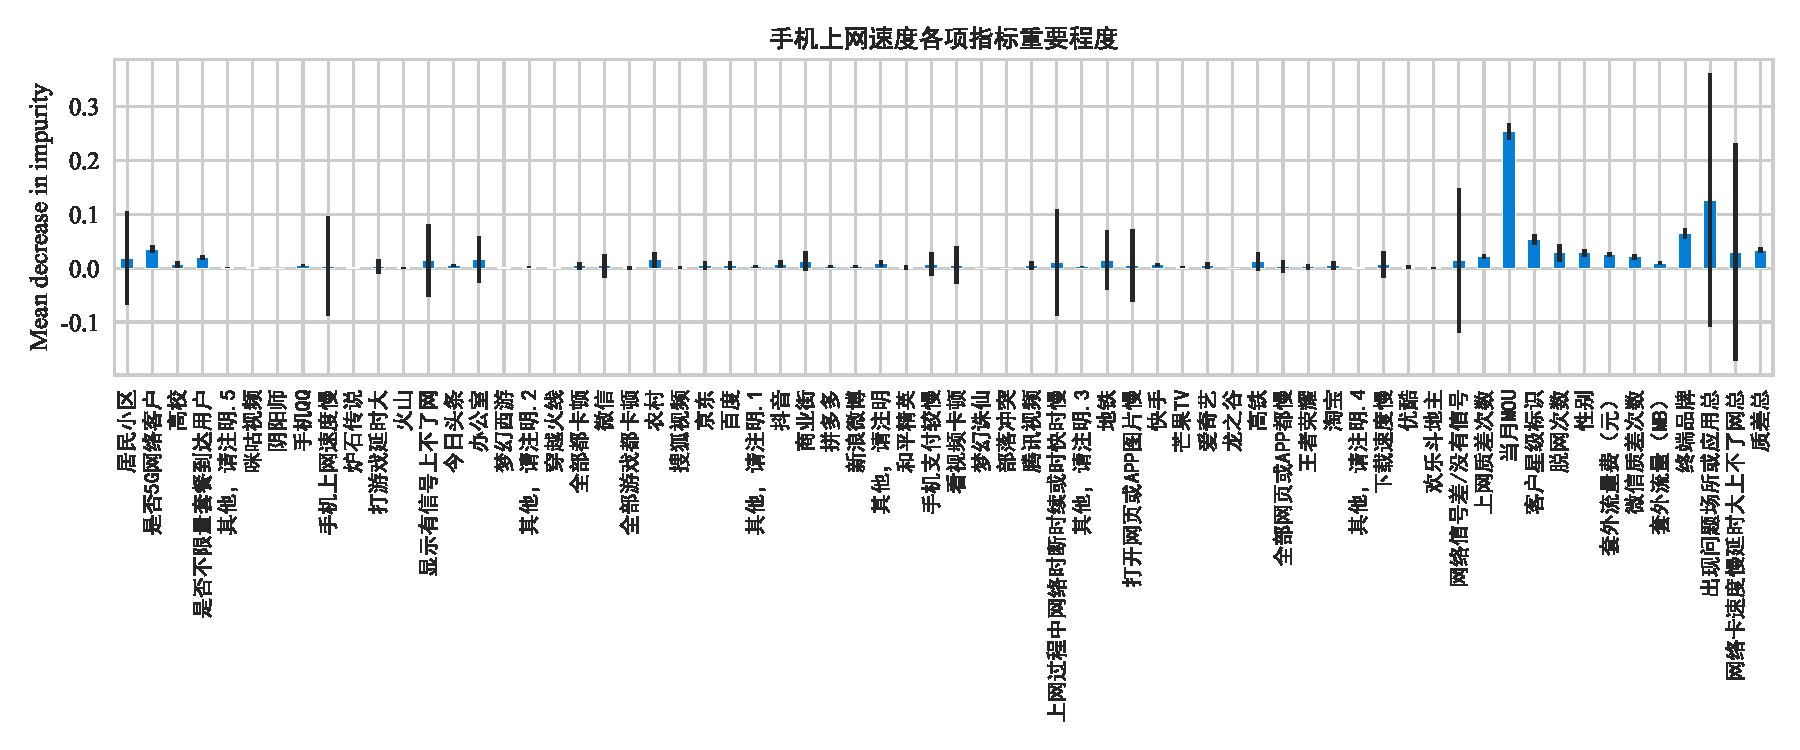
\includegraphics[scale=0.5]{[附件2]手机上网速度各项指标重要程度.pdf}}
		\caption{上网业务-手机上网速度各项指标重要程度}\label{fig:a2ThirdRF}
	\end{figure}
	\begin{figure}[H]
		\centerline{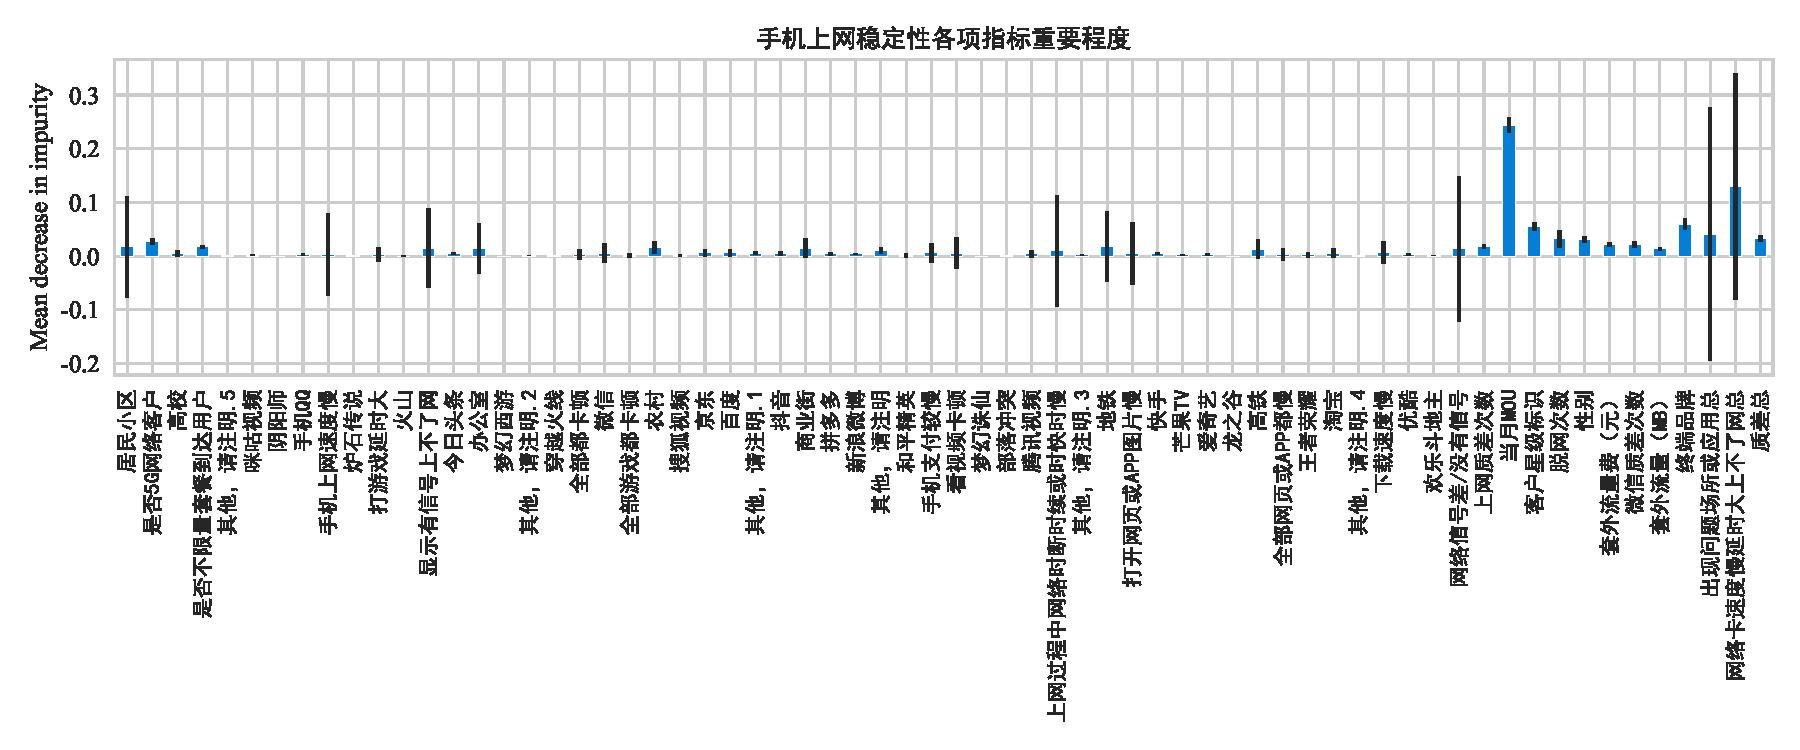
\includegraphics[scale=0.5]{[附件2]手机上网稳定性各项指标重要程度.pdf}}
		\caption{上网业务-手机上网稳定性各项指标重要程度}\label{fig:a2FourthRF}
	\end{figure}

	\begin{figure}[H]
		\centerline{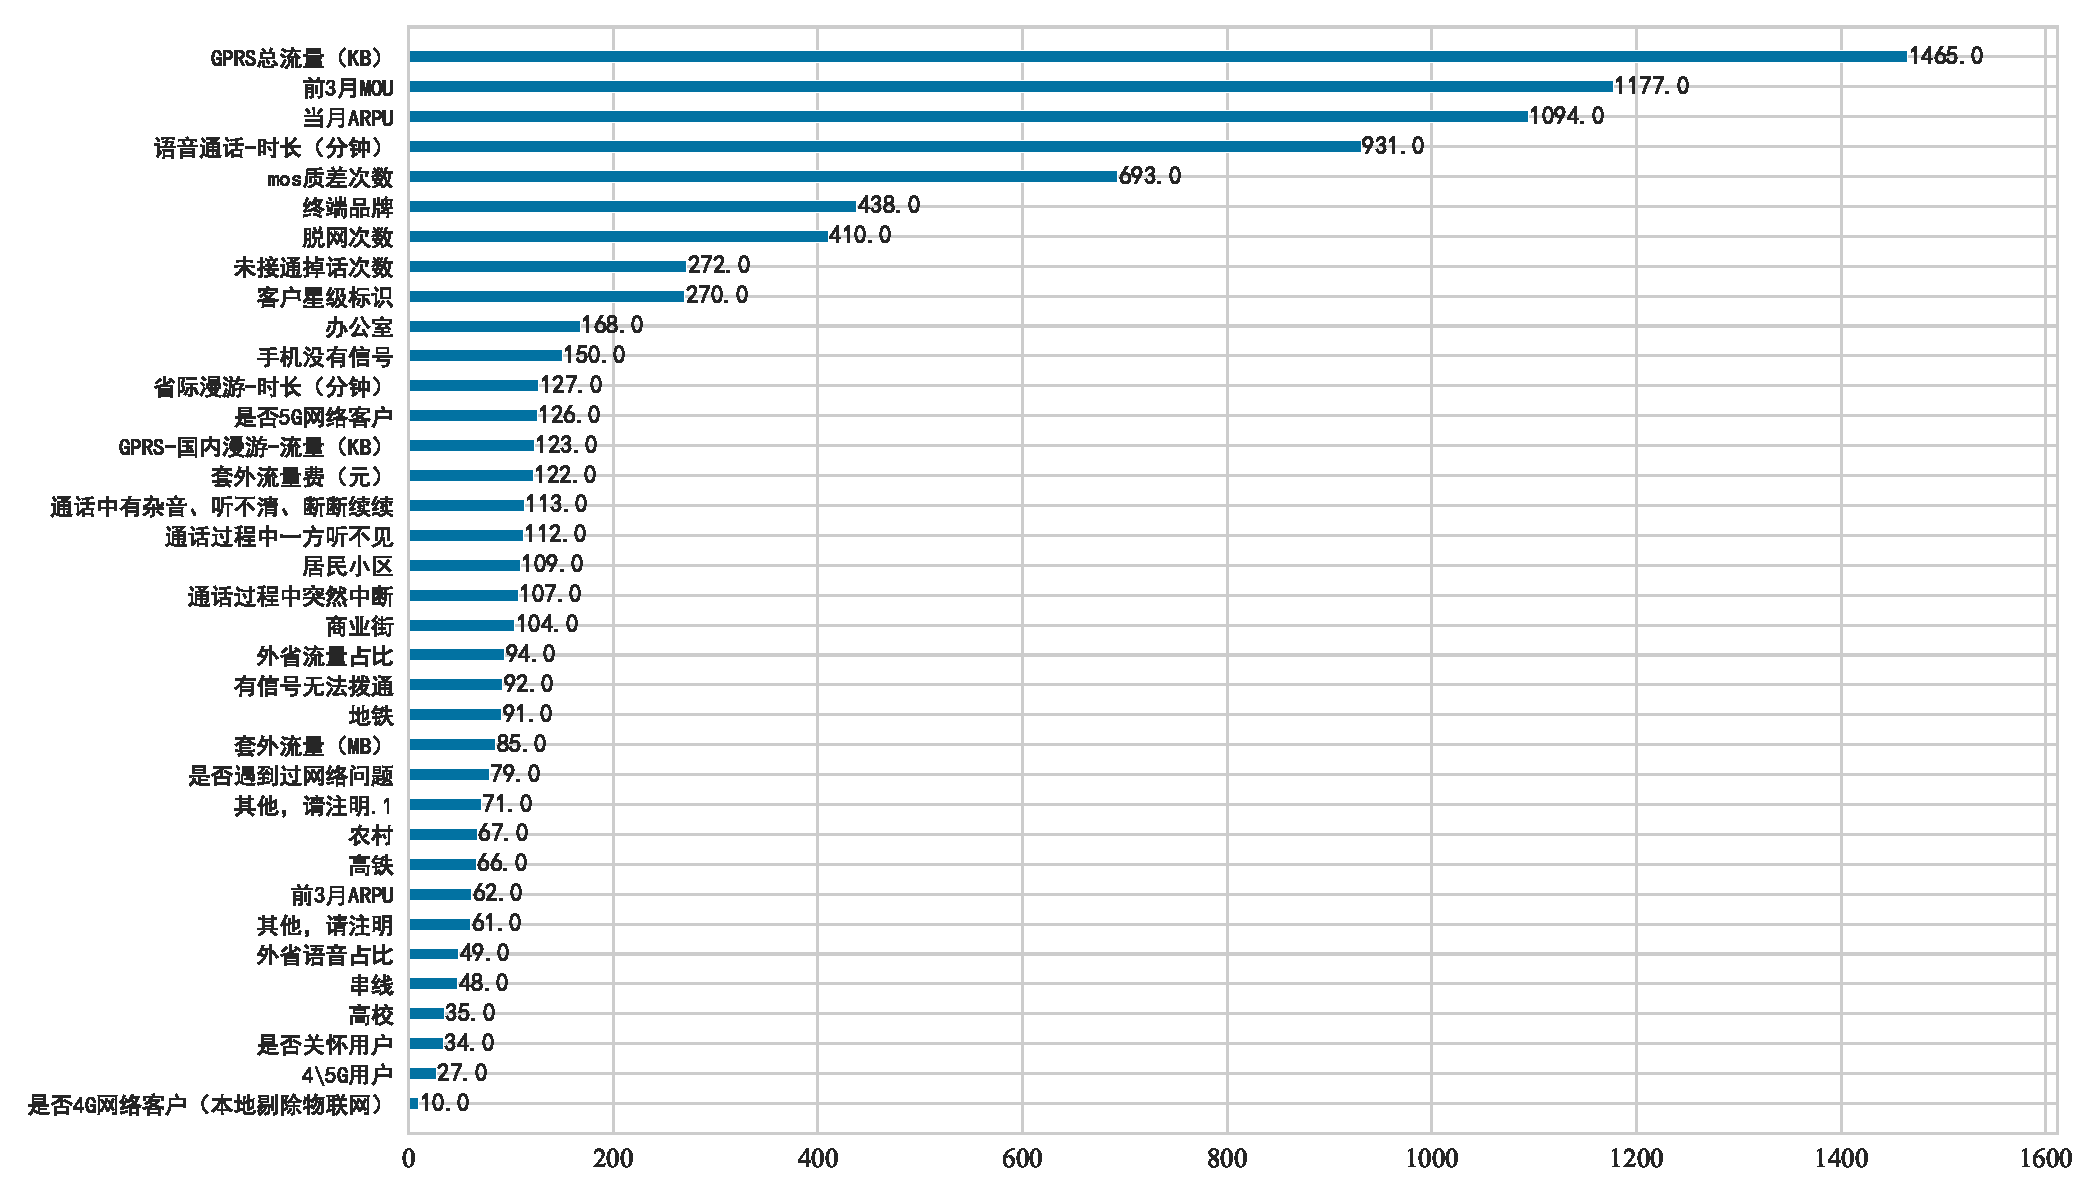
\includegraphics[scale=0.52]{[附件1]网络覆盖与信号强度各项指标重要程度(XGBoost,F-score).pdf}}
		\caption{语音业务-网络覆盖与信号强度各项指标重要程度,XGBoost}\label{fig:a1SecondXGBoost}
	\end{figure}
	\begin{figure}[H]
		\centerline{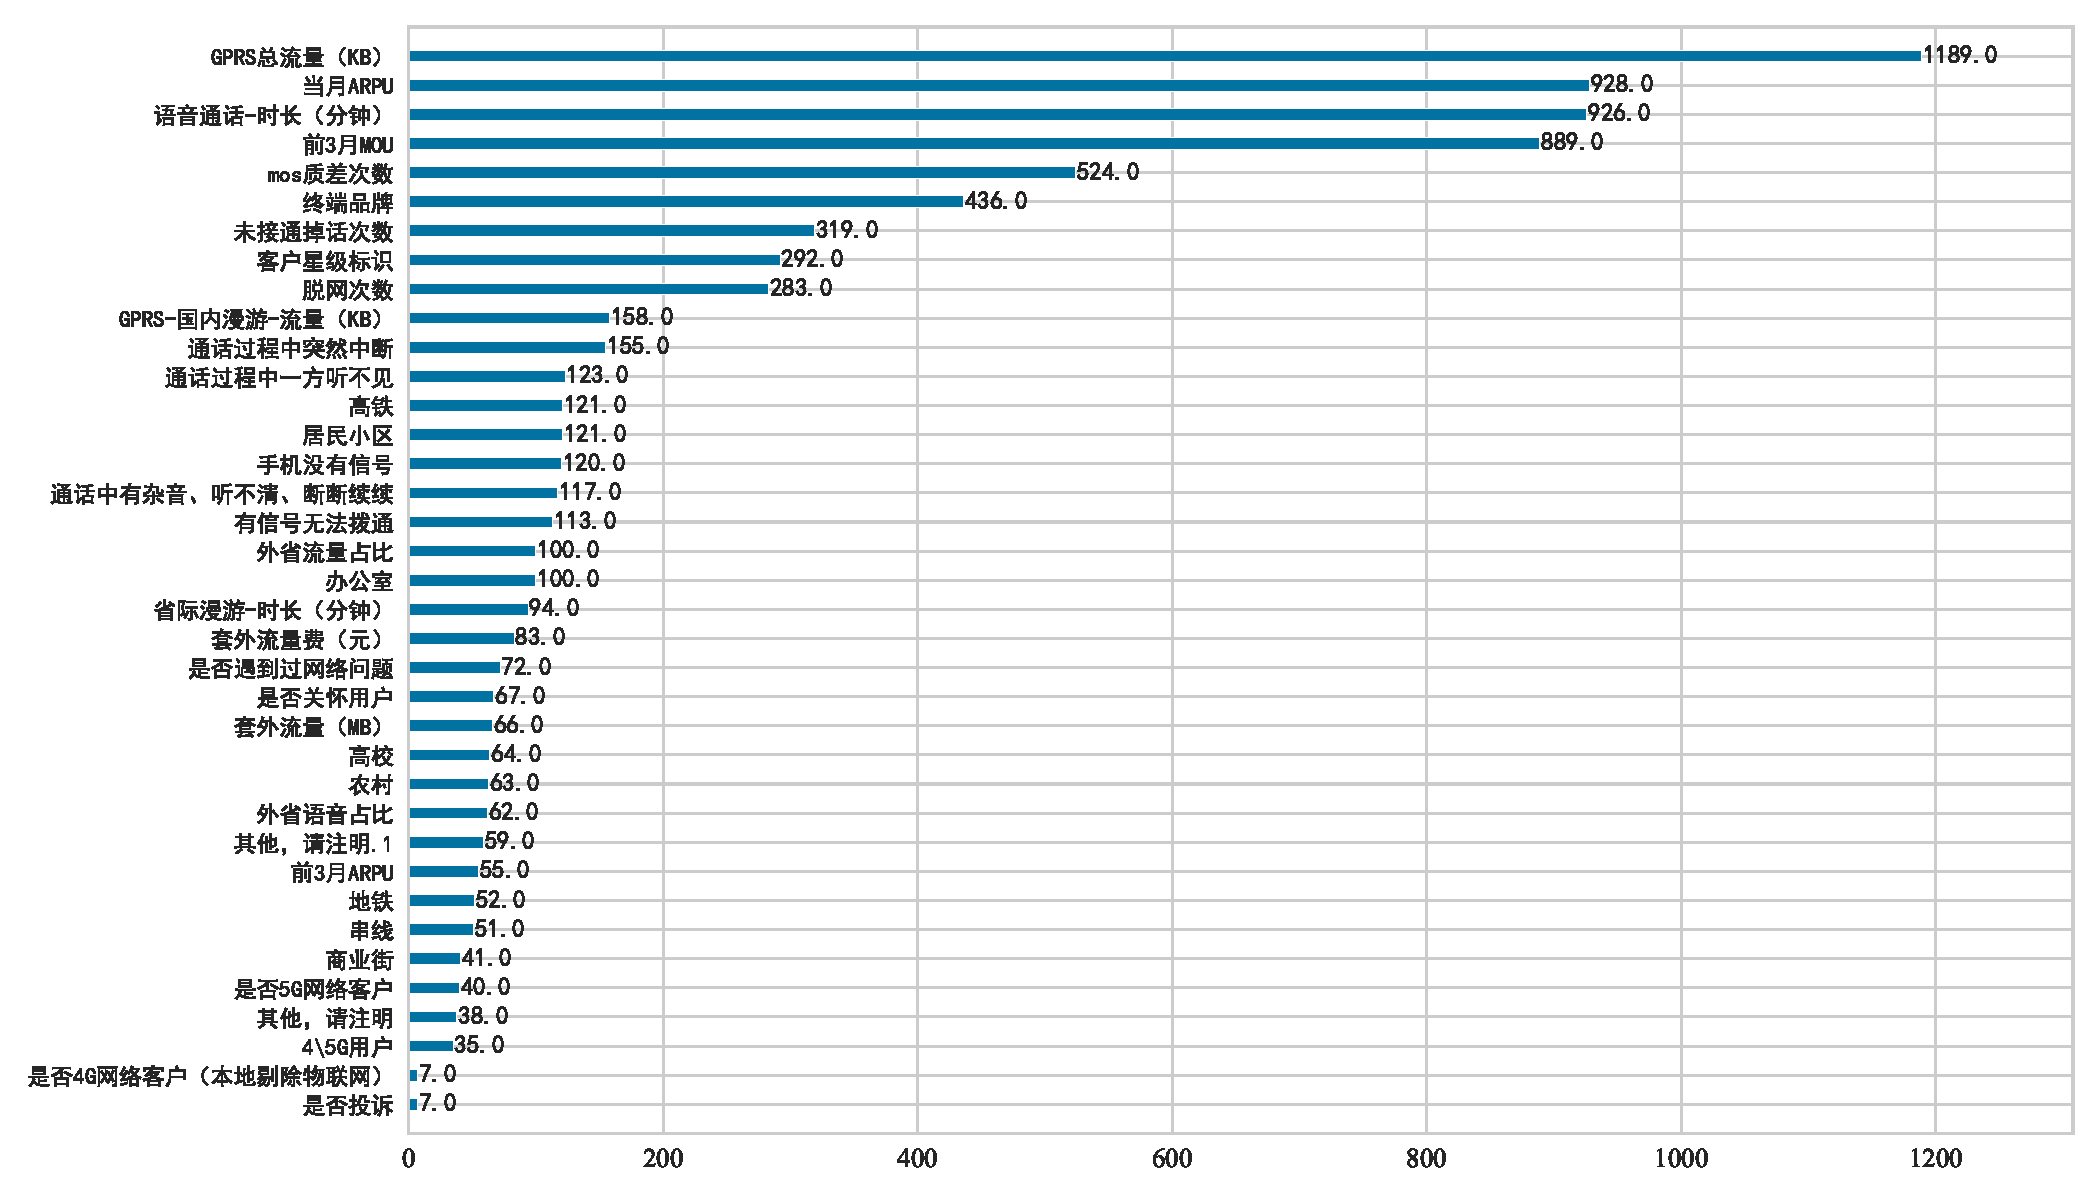
\includegraphics[scale=0.52]{[附件1]语音通话清晰度各项指标重要程度(XGBoost,F-score).pdf}}
		\caption{语音业务-语音通话清晰度各项指标重要程度,XGBoost}\label{fig:a1ThirdXGBoost}
	\end{figure}
	\begin{figure}[H]
		\centerline{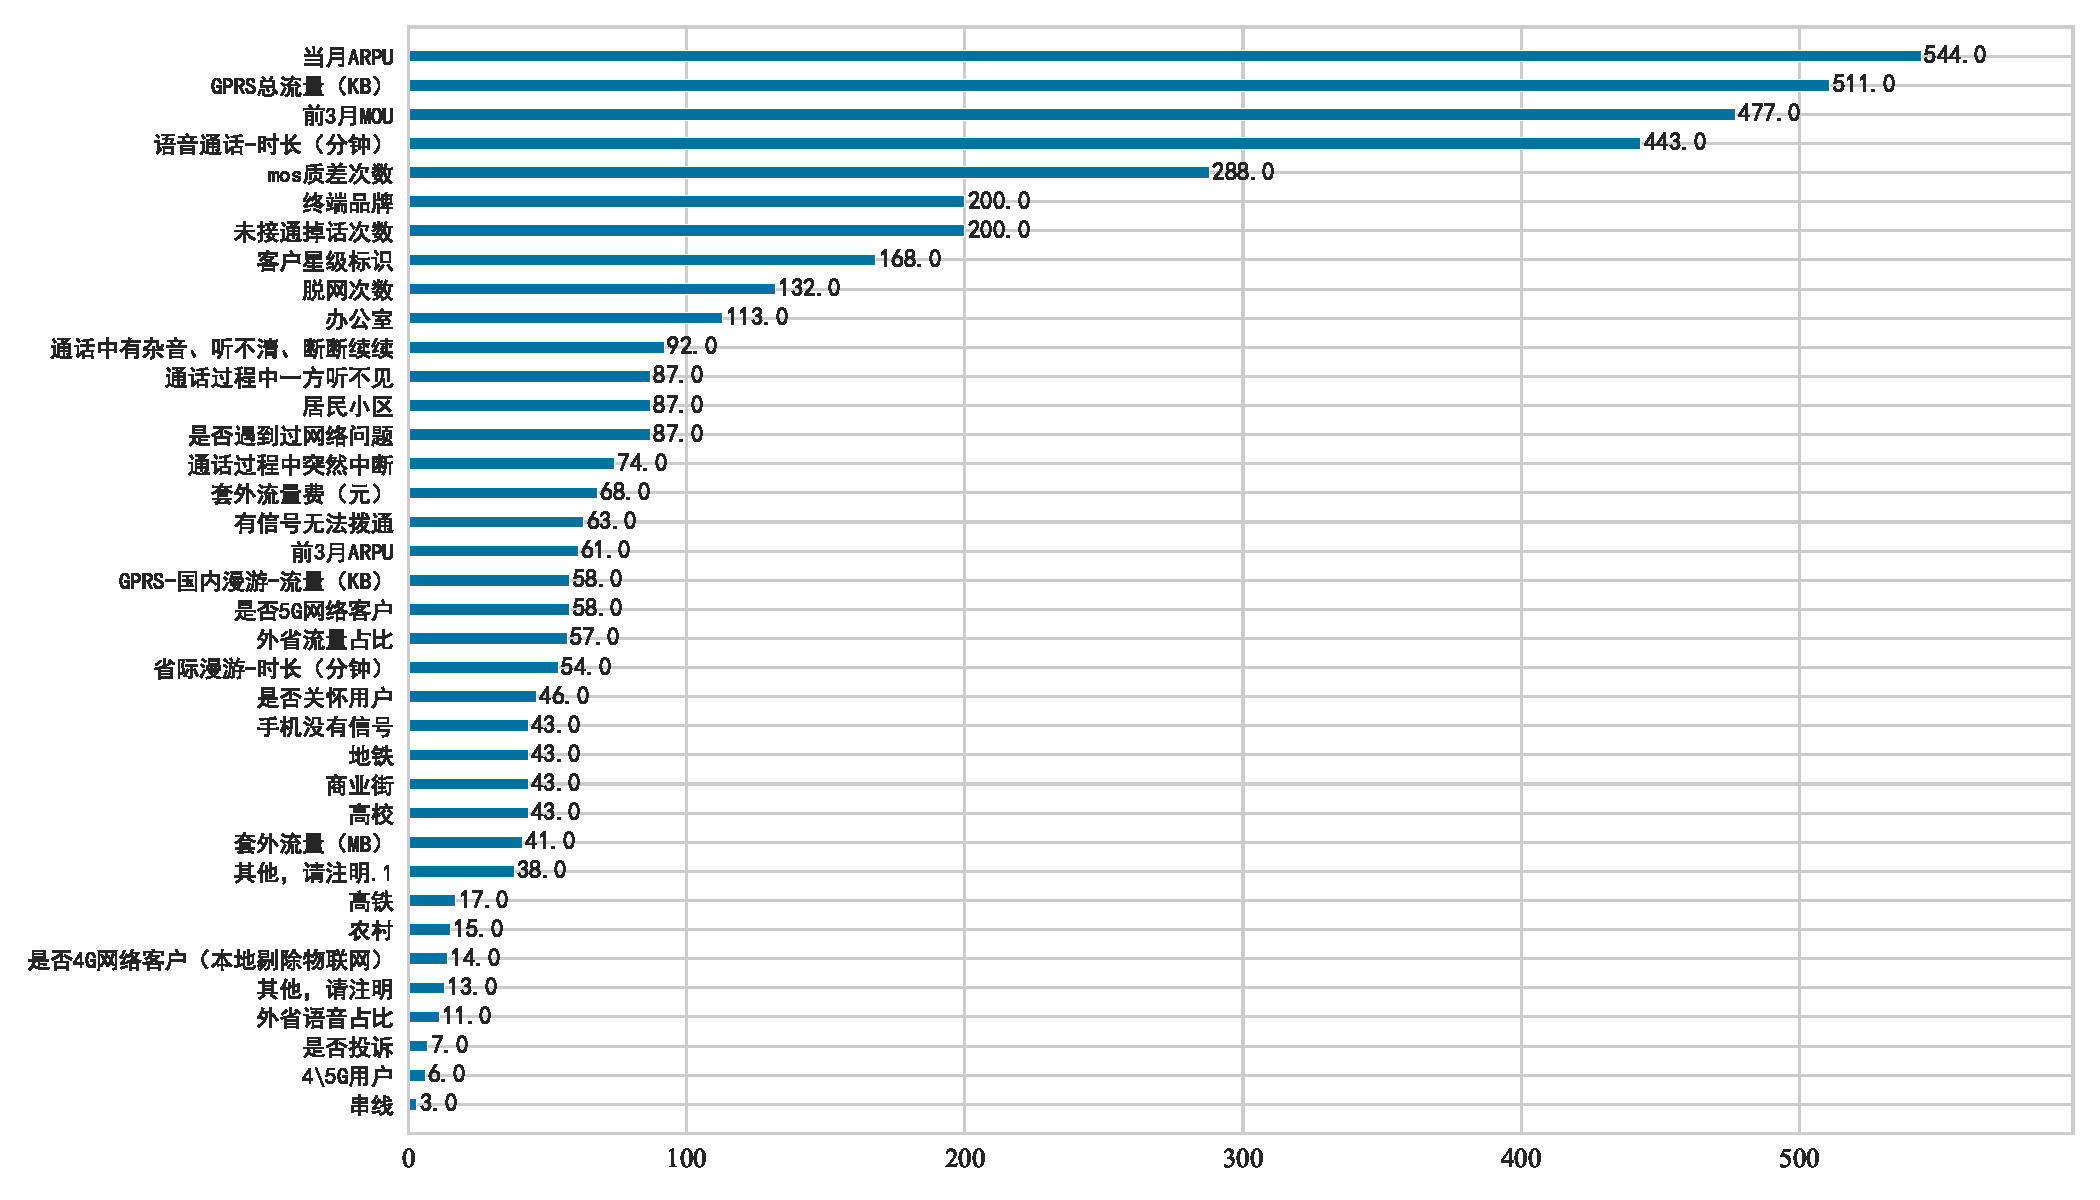
\includegraphics[scale=0.52]{[附件1]语音通话稳定性各项指标重要程度(XGBoost,F-score).pdf}}
		\caption{语音业务-语音通话稳定性各项指标重要程度,XGBoost}\label{fig:a1FourthXGBoost}
	\end{figure}
	\begin{figure}[H]
		\centerline{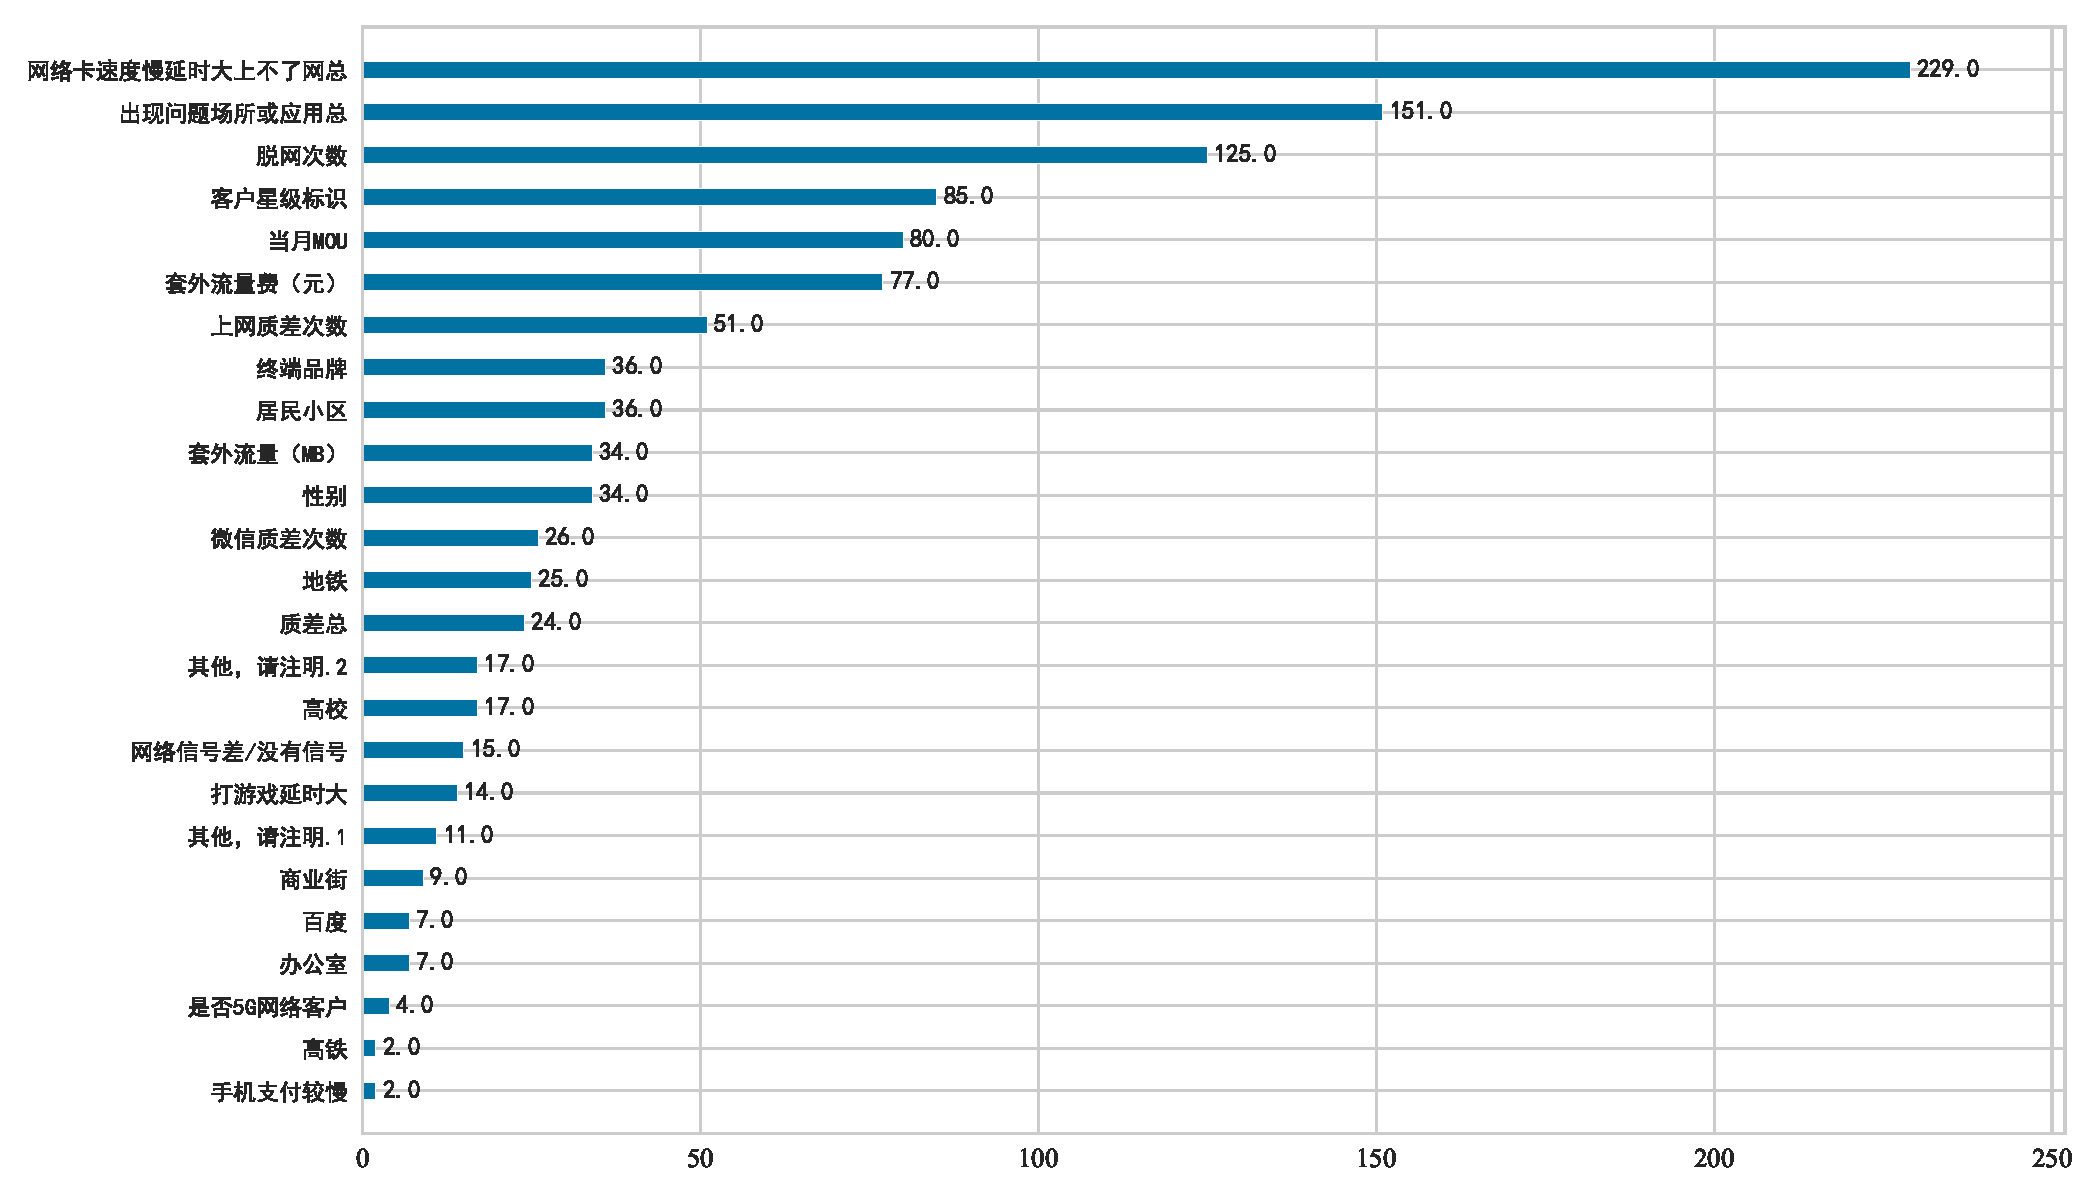
\includegraphics[scale=0.52]{[附件2]手机上网整体满意度各项指标重要程度(XGBoost,F-score).pdf}}
		\caption{上网业务-手机上网整体满意度各项指标重要程度,XGBoost}\label{fig:a2FirstXGBoost}
	\end{figure}
	\begin{figure}[H]
		\centerline{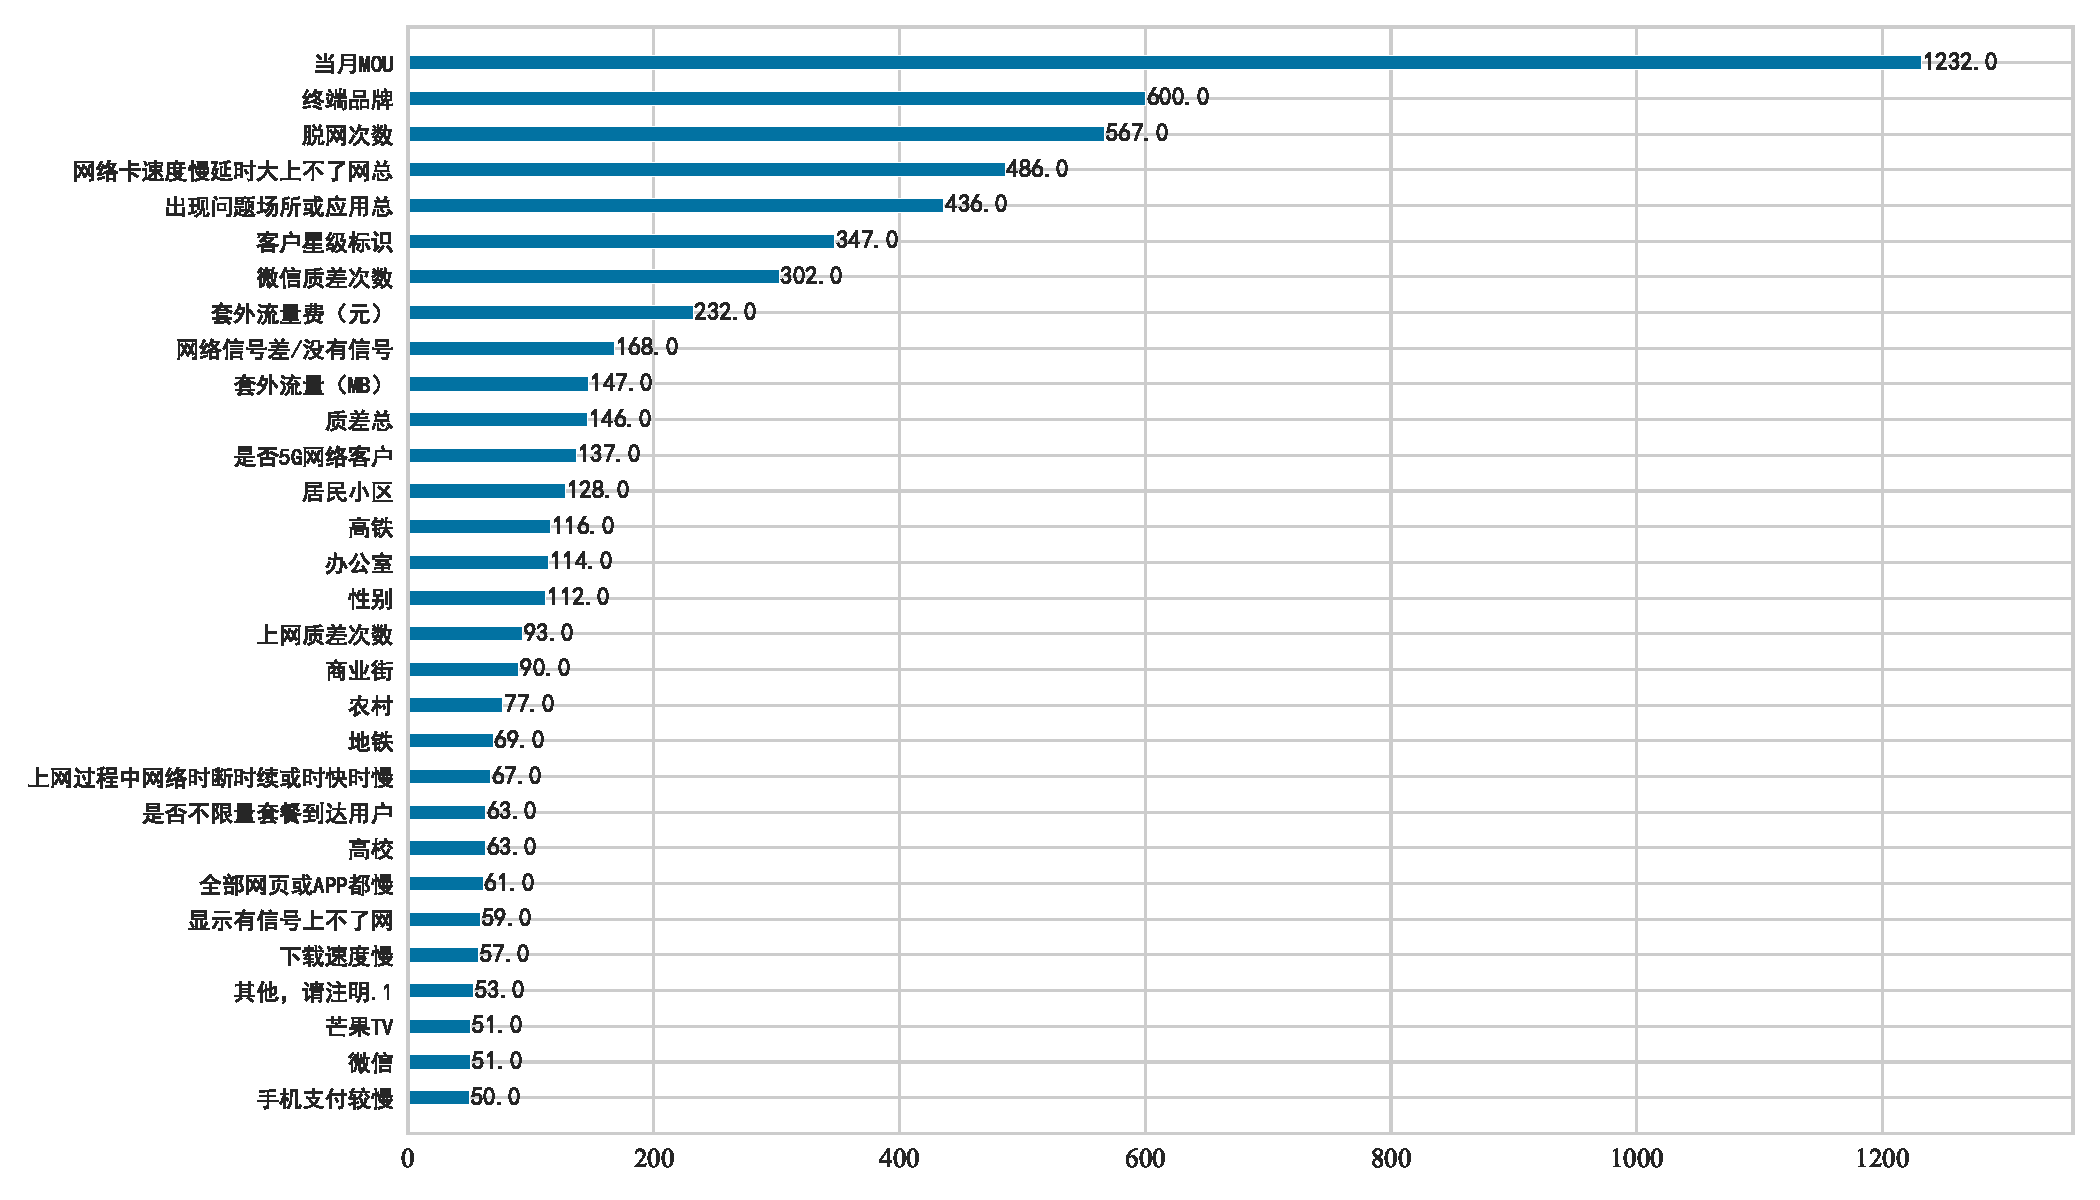
\includegraphics[scale=0.52]{[附件2]网络覆盖与信号强度各项指标重要程度(XGBoost,F-score).pdf}}
		\caption{上网业务-网络覆盖与信号强度各项指标重要程度,XGBoost}\label{fig:a2SecondXGBoost}
	\end{figure}
	\begin{figure}[H]
		\centerline{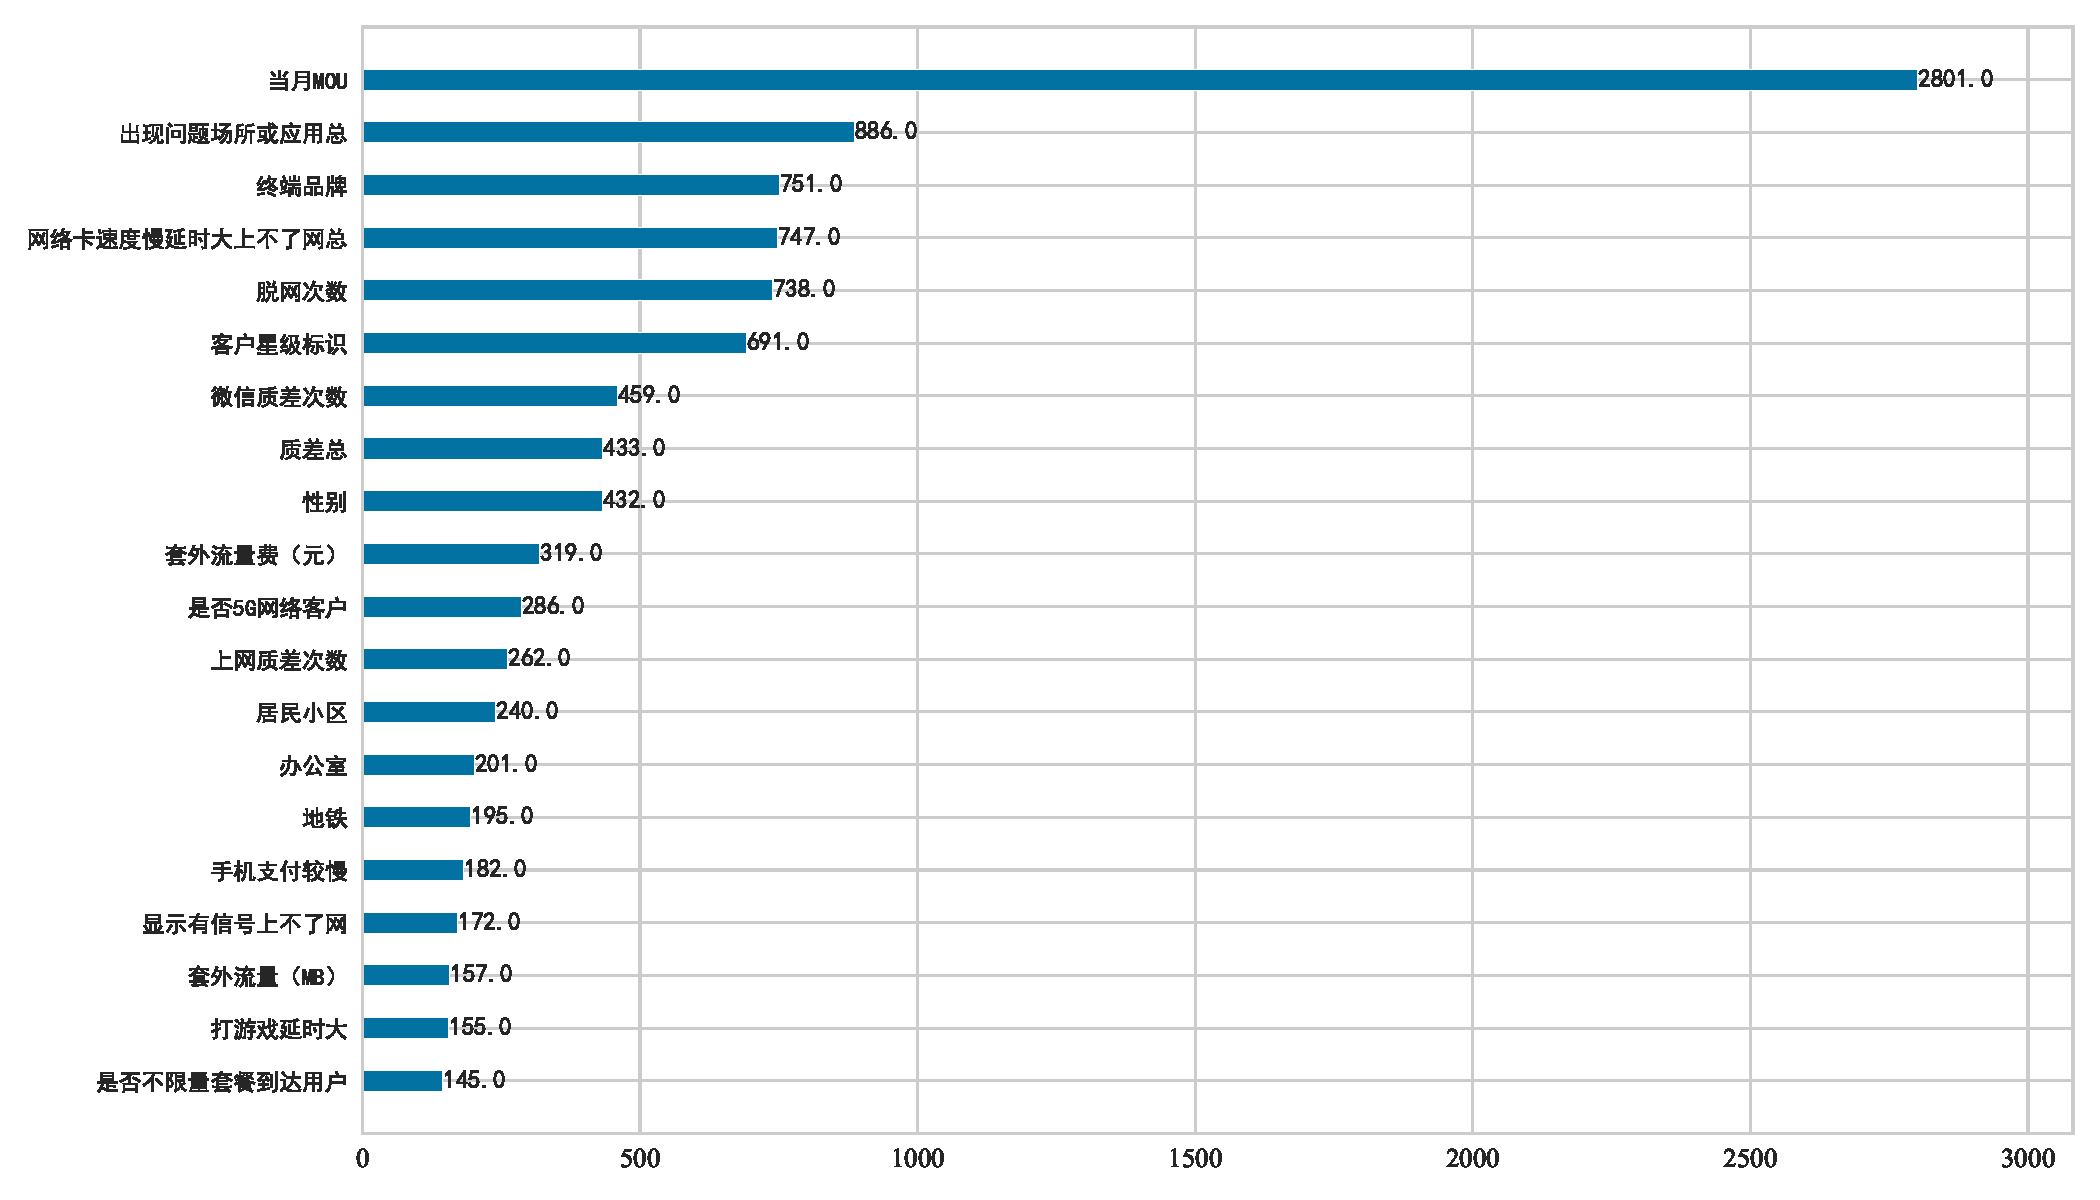
\includegraphics[scale=0.52]{[附件2]手机上网速度各项指标重要程度(XGBoost,F-score).pdf}}
		\caption{上网业务-手机上网速度各项指标重要程度,XGBoost}\label{fig:a2ThirdXGBoost}
	\end{figure}
	\begin{figure}[H]
		\centerline{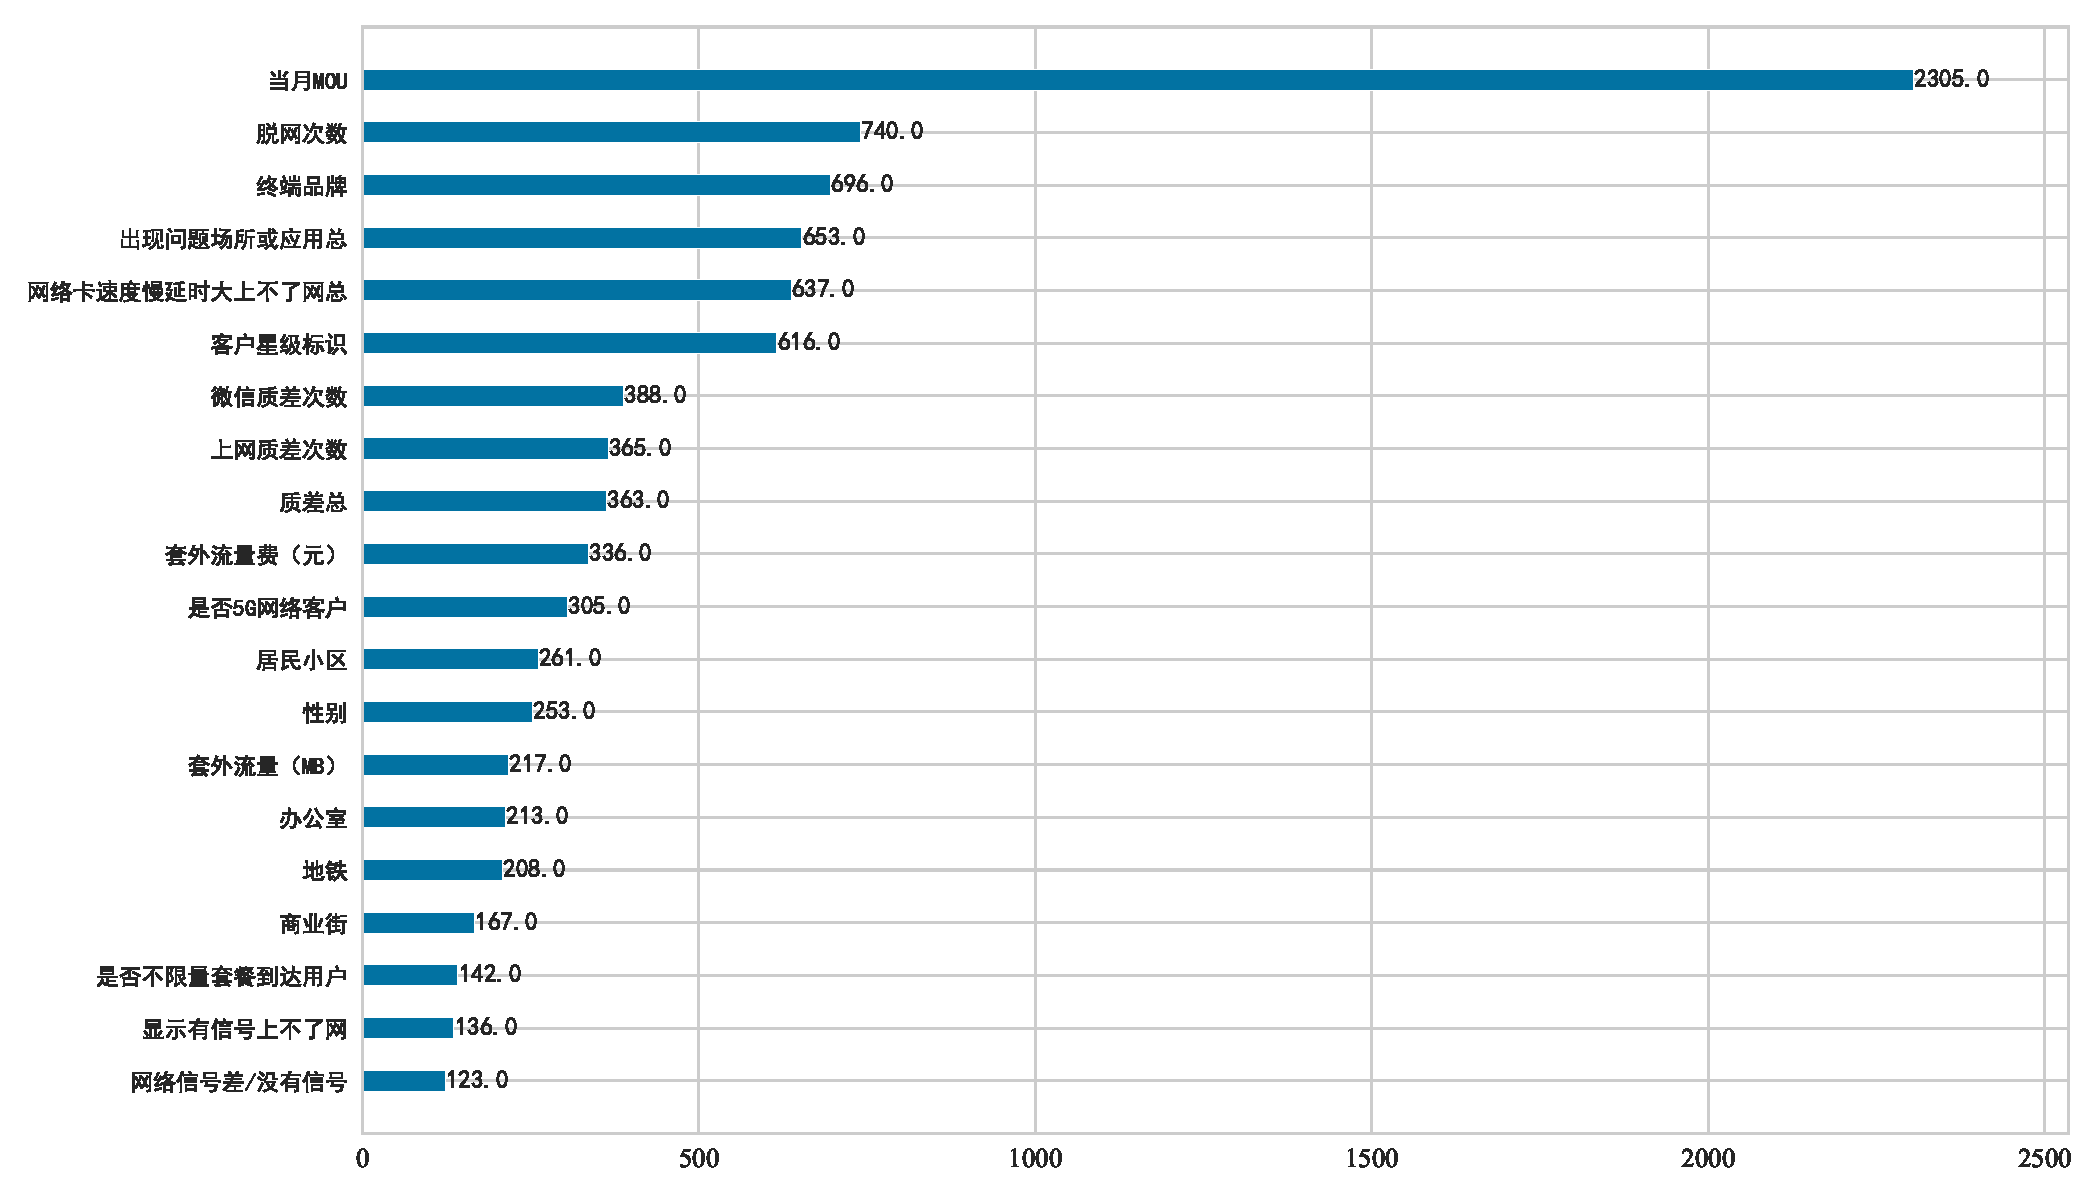
\includegraphics[scale=0.52]{[附件2]手机上网稳定性各项指标重要程度(XGBoost,F-score).pdf}}
		\caption{上网业务-手机上网稳定性各项指标重要程度,XGBoost}\label{fig:a2FourthXGBoost}
	\end{figure}
	\begin{figure}[H]
		\centerline{\includegraphics[scale=0.68]{[附件1]模型二混淆矩阵热力图.pdf}}
		\caption{模型二混淆矩阵热力图[语音业务-网络覆盖与信号强度]}\label{fig:SecondModelConfusionMatrix}
	\end{figure}
	\begin{figure}[H]
		\centerline{\includegraphics[scale=0.68]{[附件1]模型三混淆矩阵热力图.pdf}}
		\caption{模型三混淆矩阵热力图[语音业务-语音通话清晰度]}\label{fig:ThirdModelConfusionMatrix}
	\end{figure}
	\begin{figure}[H]
		\centerline{\includegraphics[scale=0.68]{[附件2]模型四混淆矩阵热力图.pdf}}
		\caption{模型四混淆矩阵热力图[语音业务-语音通话稳定性]}\label{fig:FourthModelConfusionMatrix}
	\end{figure}
	\begin{figure}[H]
		\centerline{\includegraphics[scale=0.68]{[附件2]模型一混淆矩阵热力图.pdf}}
		\caption{模型五混淆矩阵热力图[上网业务-手机上网整体满意度]}\label{fig:FifthModelConfusionMatrix}
	\end{figure}
	\begin{figure}[H]
		\centerline{\includegraphics[scale=0.68]{[附件2]模型二混淆矩阵热力图.pdf}}
		\caption{模型六混淆矩阵热力图[上网业务-网络覆盖与信号强度]}\label{fig:SixthModelConfusionMatrix}
	\end{figure}
	\begin{figure}[H]
		\centerline{\includegraphics[scale=0.68]{[附件2]模型三混淆矩阵热力图.pdf}}
		\caption{模型七混淆矩阵热力图[上网业务-手机上网速度]}\label{fig:SeventhModelConfusionMatrix}
	\end{figure}
	\begin{figure}[H]
		\centerline{\includegraphics[scale=0.68]{[附件1]模型四混淆矩阵热力图.pdf}}
		\caption{模型八混淆矩阵热力图[上网业务-手机上网稳定性]}\label{fig:EighthModelConfusionMatrix}
	\end{figure}
	\begin{figure}[H]
		\centerline{\includegraphics[scale=0.68]{[附件1]模型二分类报告.pdf}}
		\caption{模型二分类报告[语音业务-网络覆盖与信号强度]}\label{fig:SecondModelClassificationReport}
	\end{figure}
	\begin{figure}[H]
		\centerline{\includegraphics[scale=0.68]{[附件1]模型三分类报告.pdf}}
		\caption{模型三分类报告[语音业务-语音通话清晰度]}\label{fig:ThirdModelClassificationReport}
	\end{figure}
	\begin{figure}[H]
		\centerline{\includegraphics[scale=0.68]{[附件1]模型四分类报告.pdf}}
		\caption{模型四分类报告[语音业务-语音通话稳定性]}\label{fig:FourthModelClassificationReport}
	\end{figure}
	\begin{figure}[H]
		\centerline{\includegraphics[scale=0.68]{[附件2]模型一分类报告.pdf}}
		\caption{模型五分类报告[上网业务-手机上网整体满意度]}\label{fig:FifthModelClassificationReport}
	\end{figure}
	\begin{figure}[H]
		\centerline{\includegraphics[scale=0.68]{[附件2]模型二分类报告.pdf}}
		\caption{模型六分类报告[上网业务-网络覆盖与信号强度]}\label{fig:SixthModelClassificationReport}
	\end{figure}
	\begin{figure}[H]
		\centerline{\includegraphics[scale=0.68]{[附件2]模型三分类报告.pdf}}
		\caption{模型七分类报告[上网业务-手机上网速度]}\label{fig:SeventhModelClassificationReport}
	\end{figure}
	\begin{figure}[H]
		\centerline{\includegraphics[scale=0.68]{[附件2]模型四分类报告.pdf}}
		\caption{模型八分类报告[上网业务-手机上网稳定性]}\label{fig:EighthModelClassificationReport}
	\end{figure}
	\begin{figure}[H]
		\centerline{\includegraphics[scale=0.68]{[附件1]模型二ROCAUC.pdf}}
		\caption{模型二ROC/AUC曲线[语音业务-网络覆盖与信号强度]}\label{fig:SecondModelROCAUC}
	\end{figure}
	\begin{figure}[H]
		\centerline{\includegraphics[scale=0.68]{[附件1]模型三ROCAUC.pdf}}
		\caption{模型三ROC/AUC曲线[语音业务-语音通话清晰度]}\label{fig:ThirdModelROCAUC}
	\end{figure}
	\begin{figure}[H]
		\centerline{\includegraphics[scale=0.68]{[附件1]模型四ROCAUC.pdf}}
		\caption{模型四ROC/AUC曲线[语音业务-语音通话稳定性]}\label{fig:FourthModelROCAUC}
	\end{figure}
	\begin{figure}[H]
		\centerline{\includegraphics[scale=0.68]{[附件2]模型一ROCAUC.pdf}}
		\caption{模型五ROC/AUC曲线[上网业务-手机上网整体满意度]}\label{fig:FifthModelROCAUC}
	\end{figure}
	\begin{figure}[H]
		\centerline{\includegraphics[scale=0.68]{[附件2]模型二ROCAUC.pdf}}
		\caption{模型六ROC/AUC曲线[上网业务-网络覆盖与信号强度]}\label{fig:SixthModelROCAUC}
	\end{figure}
	\begin{figure}[H]
		\centerline{\includegraphics[scale=0.68]{[附件2]模型三ROCAUC.pdf}}
		\caption{模型七ROC/AUC曲线[上网业务-手机上网速度]}\label{fig:SeventhModelROCAUC}
	\end{figure}
	\begin{figure}[H]
		\centerline{\includegraphics[scale=0.68]{[附件2]模型四ROCAUC.pdf}}
		\caption{模型八ROC/AUC曲线[上网业务-手机上网稳定性]}\label{fig:EighthModelROCAUC}
	\end{figure}

	\begin{table}[H]
		\centering
		\caption{语音业务熵权法关联分析影响程度量化结果}
		\setlength{\aboverulesep}{0pt}
		\setlength{\belowrulesep}{0pt}
		\scalebox{0.72}{
		\begin{tabular}{cc||cc}
		\toprule
		\textbf{因素} & \textbf{量化值} & \textbf{因素} & \textbf{量化值} \\
		\midrule
		省际漫游-时长(分钟)  & 0.1404  & 有信号无法拨通  & 0.0398  \\
		前3月ARPU  & 0.1360  & 办公室   & 0.0364  \\
		套外流量(MB)  & 0.1330  & 地铁    & 0.0345  \\
		GPRS-国内漫游-流量(KB)  & 0.1288  & 通话过程中突然中断  & 0.0312  \\
		套外流量费(元)  & 0.1232  & 手机没有信号  & 0.0306  \\
		脱网次数  & 0.0848  & 通话过程中一方听不见  & 0.0305  \\
		其他,请注明.1  & 0.0777  & 通话中有杂音、听不清、断断续续  & 0.0279  \\
		未接通掉话次数 & 0.0773  & GPRS总流量(KB)  & 0.0255  \\
		高校    & 0.0770  & 居民小区  & 0.0251  \\
		是否投诉  & 0.0741  & 语音通话-时长(分钟)  & 0.0246  \\
		是否关怀用户  & 0.0700  & 当月MOU  & 0.0246  \\
		串线    & 0.0690  & 是否5G网络客户 & 0.0222  \\
		其他,请注明  & 0.0648  & 前3月MOU  & 0.0220  \\
		外省语音占比  & 0.0591  & 当月ARPU  & 0.0180  \\
		外省流量占比  & 0.0586  & 是否遇到过网络问题  & 0.0150  \\
		商业街   & 0.0560  & 4\textbackslash{}\textbackslash{}5G用户 & 0.0045  \\
		农村    & 0.0535  & 终端品牌  & 0.0039  \\
		mos质差次数 & 0.0512  & 客户星级标识 & 0.0021  \\
		高铁    & 0.0469  & 是否4G网络客户(本地剔除物联网)  & 0.0001  \\
		\bottomrule
		\end{tabular}}
		\label{tab:a1ewm}
	\end{table}
	\begin{table}[H]
		\centering
		\caption{语音业务灰度关联分析影响程度量化结果}
		\setlength{\aboverulesep}{0pt}
		\setlength{\belowrulesep}{0pt}
		\scalebox{0.72}{
		  \begin{tabular}{cc||cc}
		  \toprule
		  \textbf{因素} & \textbf{量化值} & \textbf{因素} & \textbf{量化值} \\
		  \midrule
		  前3月ARPU & 0.9920  & 商业街   & 0.9424  \\
		  套外流量(MB) & 0.9918  & 农村    & 0.9351  \\
		  套外流量费(元) & 0.9890  & mos质差次数 & 0.9275  \\
		  GPRS-国内漫游-流量(KB) & 0.9878  & 高铁    & 0.9123  \\
		  脱网次数  & 0.9858  & 有信号无法拨通 & 0.8797  \\
		  省际漫游-时长(分钟) & 0.9856  & 办公室   & 0.8603  \\
		  其他,请注明.1 & 0.9827  & 当月ARPU & 0.8487  \\
		  高校    & 0.9819  & 地铁    & 0.8482  \\
		  未接通掉话次数 & 0.9790  & 通话过程中突然中断 & 0.8244  \\
		  GPRS总流量(KB) & 0.9781  & 手机没有信号 & 0.8200  \\
		  是否投诉  & 0.9777  & 通话过程中一方听不见 & 0.8192  \\
		  是否关怀用户 & 0.9716  & 通话中有杂音、听不清、断断续续 & 0.7973  \\
		  串线    & 0.9699  & 居民小区  & 0.7711  \\
		  前3月MOU & 0.9683  & 是否5G网络客户 & 0.7416  \\
		  语音通话-时长(分钟) & 0.9671  & 是否遇到过网络问题 & 0.6471  \\
		  当月MOU & 0.9671  & 客户星级标识 & 0.4986  \\
		  其他,请注明 & 0.9626  & 终端品牌  & 0.4616  \\
		  外省语音占比 & 0.9556  & 4\textbackslash{}5G用户 & 0.4386  \\
		  外省流量占比 & 0.9546  & 是否4G网络客户(本地剔除物联网) & 0.3375  \\
		  \bottomrule
		  \end{tabular}}
		\label{tab:a1grey}
	\end{table}
	\begin{table}[H]
		\centering
		\caption{上网业务主要因素及其量化结果,EWM及灰色关联分析}
		\setlength{\aboverulesep}{0pt}
		\setlength{\belowrulesep}{0pt}
		\scalebox{0.6}{
		  \begin{tabular}{ccc||ccc}
		  \toprule
		  \textbf{因素} & \textbf{EWM量化} & \textbf{灰色关联度量化} & \textbf{因素} & \textbf{EWM量化} & \textbf{灰色关联度量化} \\
		  \midrule
		  套外流量(MB) & 0.0238  & 0.9891  & 新浪微博  & 0.0164  & 0.9415  \\
		  其他,请注明.5 & 0.0238  & 0.9893  & 爱奇艺   & 0.0164  & 0.9948  \\
		  火山    & 0.0238  & 0.9895  & 梦幻诛仙  & 0.0160  & 0.9370  \\
		  全部都卡顿 & 0.0238  & 0.9897  & 脱网次数  & 0.0155  & 0.9323  \\
		  拼多多   & 0.0236  & 0.9863  & 打开网页或APP图片慢 & 0.0139  & 0.9129  \\
		  王者荣耀  & 0.0235  & 0.9856  & 部落冲突  & 0.0136  & 0.9087  \\
		  优酷    & 0.0234  & 0.9852  & 是否不限量套餐到达用户 & 0.0132  & 0.9040  \\
		  咪咕视频  & 0.0234  & 0.9851  & 商业街   & 0.0132  & 0.9039  \\
		  全部游戏都卡顿 & 0.0232  & 0.9918  & 套外流量费(元) & 0.0132  & 0.9036  \\
		  京东    & 0.0231  & 0.9839  & 上网质差次数 & 0.0129  & 0.8989  \\
		  性别    & 0.0231  & 0.9920  & 搜狐视频  & 0.0127  & 0.8960  \\
		  看视频卡顿 & 0.0229  & 0.9829  & 抖音    & 0.0118  & 0.9865  \\
		  地铁    & 0.0228  & 0.9824  & 快手    & 0.0112  & 0.8690  \\
		  其他,请注明.2 & 0.0220  & 0.9930  & 手机支付较慢 & 0.0104  & 0.9929  \\
		  上网过程中网络时断时续或时快时慢 & 0.0207  & 0.9721  & 梦幻西游  & 0.0103  & 0.9893  \\
		  客户星级标识 & 0.0207  & 0.9718  & 办公室   & 0.0097  & 0.8380  \\
		  手机QQ  & 0.0206  & 0.9717  & 其他,请注明.4 & 0.0091  & 0.8232  \\
		  下载速度慢 & 0.0206  & 0.9715  & 百度    & 0.0087  & 0.9909  \\
		  腾讯视频  & 0.0205  & 0.9709  & 淘宝    & 0.0081  & 0.7952  \\
		  龙之谷   & 0.0203  & 0.9938  & 显示有信号上不了网 & 0.0080  & 0.7898  \\
		  高校    & 0.0202  & 0.9689  & 质差总   & 0.0077  & 0.9864  \\
		  微信质差次数 & 0.0201  & 0.9685  & 手机上网速度慢 & 0.0076  & 0.7778  \\
		  炉石传说  & 0.0200  & 0.9939  & 其他,请注明 & 0.0072  & 0.9899  \\
		  农村    & 0.0196  & 0.9654  & 居民小区  & 0.0066  & 0.7422  \\
		  其他,请注明.3 & 0.0189  & 0.9612  & 全部网页或APP都慢 & 0.0065  & 0.7389  \\
		  今日头条  & 0.0187  & 0.9601  & 终端品牌  & 0.0056  & 0.7044  \\
		  网络信号差/没有信号 & 0.0183  & 0.9944  & 是否5G网络客户 & 0.0054  & 0.6964  \\
		  欢乐斗地主 & 0.0182  & 0.9561  & 出现问题场所或应用总 & 0.0049  & 0.8886  \\
		  阴阳师   & 0.0179  & 0.9945  & 网络卡速度慢延时大上不了网总 & 0.0047  & 0.7801  \\
		  高铁    & 0.0175  & 0.9507  & 穿越火线  & 0.0041  & 0.9102  \\
		  当月MOU & 0.0175  & 0.9507  & 其他,请注明.1 & 0.0028  & 0.5579  \\
		  打游戏延时大 & 0.0172  & 0.9485  & 芒果TV  & 0.0015  & 0.8814  \\
		  和平精英  & 0.0166  & 0.9431  & 微信    & 0.0003  & 0.5094  \\
		  \bottomrule
		  \end{tabular}}
		\label{tab:a2ewmgrey}
	\end{table}
\newpage
% \phantomsection
% \addcontentsline{toc}{subsection}{[B]支撑文件列表}
% 	% \section*{[B]支撑文件列表}
	\noindent{\heiti [B]支撑文件列表}
	~\\

	支撑文件列表如下(列表中不包含原始数据集):
	% Table generated by Excel2LaTeX from sheet 'Sheet2'
	\begin{table}[htbp]
	\centering
	\scalebox{0.88}{
	  \begin{tabular}{cc}
	  \toprule
	  \textbf{文件(夹)名} & \textbf{描述} \\
	  \midrule
	  result.xlsx & 用户评分预测结果 \\
	  所有量化结果.xlsx & 问题一量化结果 \\
	  模型参数.xlsx & 各个模型评估参数以及模型选择依据 \\
	  语音业务词云.txt & 语音业务词云图文本内容 \\
	  上网业务词云.txt & 上网业务词云图文本内容 \\
	  语音业务数据分析.ipynb & 语音业务分析Jupyter文件 \\
	  上网业务数据分析.ipynb & 上网业务分析Jupyter文件 \\
	  语音业务数据分析.html & 语音业务分析运行结果 \\
	  上网业务数据分析.html & 上网业务分析运行结果 \\
	  bg.jpg & 词语底图 \\
	  figuresNightingaleRoseDiagramF.py & 原始数据用户评分南丁格尔玫瑰图程序 \\
	  figuresNightingaleRoseDiagramP.py & 预测数据用户评分南丁格尔玫瑰图程序 \\
	  figuresOne & 语音业务所有图示文件夹 \\
	  figuresTwo & 上网业务所有图示文件夹 \\
	  figuresNightingaleRoseDiagramF & 原始数据用户评分南丁格尔玫瑰图示(八项评分) \\
	  figuresNightingaleRoseDiagramP & 预测数据用户评分南丁格尔玫瑰图示(八项评分) \\
	  \bottomrule
	  \end{tabular}}
  	\end{table}
  
\newpage
% \phantomsection
% \addcontentsline{toc}{subsection}{[C]使用的软件、环境}
	% \section*{[C]使用的软件、环境}
	\noindent{\heiti [C]使用的软件、环境}
	~\\

	为解决该问题,我们所使用的主要软件有:
	\begin{itemize}
		\item TeX Live 2022
		\item Visual Studio Code 1.74.2
		\item WPS Office 2022冬季更新(13703)
		\item Python 3.10.4
		\item Pycharm Professional 2022.3
	\end{itemize}
	
	Python环境下所用使用到的库及其版本如下:
\begin{table}[htbp]
	\centering
	\setlength{\aboverulesep}{0pt}
	\setlength{\belowrulesep}{0pt}
	\scalebox{0.88}{
	  \begin{tabular}{cc||cc}
	  \toprule
	  \textbf{库} & \textbf{版本} & \textbf{库} & \textbf{版本} \\
	  \midrule
	  copy  & 内置库   & missingno & 0.5.1 \\
	  jieba & 0.42.1 & mlxtend & 0.20.2 \\
	  jupyter & 1.0.0 & numpy & 1.22.4+mkl \\
	  jupyter-client & 7.3.1 & openpyxl & 3.0.10 \\
	  jupyter-console & 6.4.3 & pandas & 1.4.2 \\
	  jupyter-contrib-core & 0.4.0 & pyecharts & 1.9.1 \\
	  jupyter-contrib-nbextensions & 0.5.1 & scikit-learn & 0.22.2.post1 \\
	  jupyter-core & 4.10.0 & seaborn & 0.11.2 \\
	  jupyter-highlight-selected-word & 0.2.0 & sklearn & 0.0  \\
	  jupyterlab-pygments & 0.2.2 & snapshot\_phantomjs & 0.0.3 \\
	  jupyterlab-widgets & 1.1.0 & warnings & 内置库 \\
	  jupyter-latex-envs & 1.4.6 & wordcloud & 1.8.1 \\
	  jupyter-nbextensions-configurator & 0.5.0 & xgboost & 1.6.1 \\
	  matplotlib & 3.5.2 & yellowbrick & 1.4 \\
	  \bottomrule
	  \end{tabular}}
\end{table}

\newpage
% \phantomsection
% \addcontentsline{toc}{subsection}{[D]问题解决源程序}
	% \section*{[D]问题解决源程序}
\noindent{\heiti [D]问题解决源程序}

% \phantomsection
% \addcontentsline{toc}{subsubsection}{D.1 语音业务分析代码[针对附件1与附件3]}
\textbf{D.1 语音业务分析代码[针对附件1与附件3]}
\begin{python}
	#!/usr/bin/env python
	# coding: utf-8
	
	# # 2022 MathorCup 大数据 IssueB
	
	# # 语音业务数据分析
	
	# ## 初步导入相关第三方库
	
	# In[1]:
	
	
	import pandas as pd
	import numpy as np
	import sklearn.preprocessing as sp
	import warnings
	
	warnings.filterwarnings("ignore")
	
	# ## 读取附件1与附件3
	
	# In[2]:
	
	
	dataOne = pd.read_excel("附件1语音业务用户满意度数据.xlsx", sheet_name='Sheet1')
	dataThree = pd.read_excel("附件3语音业务用户满意度预测数据.xlsx", sheet_name='语音')
	
	# In[3]:
	
	
	dataOne
	
	# In[4]:
	
	
	dataThree
	
	# ## 处理附件1与附件3
	
	# ### 查看附件1与附件3表头
	
	# In[5]:
	
	
	dataOneColumnsList = list(dataOne.columns)
	dataThreeColumnsList = list(dataThree.columns)
	
	# In[6]:
	
	
	dataOneColumnsList
	
	# In[7]:
	
	
	dataThreeColumnsList
	
	# In[8]:
	
	
	set(dataOneColumnsList) & set(dataThreeColumnsList)
	
	# In[9]:
	
	
	set(dataOneColumnsList) - set(dataThreeColumnsList)
	
	# ### 对附件1增加一项指标[是否投诉],来源于[家宽投诉 与 资费投诉],并删除[家宽投诉 与 资费投诉]
	
	# In[10]:
	
	
	dataOne['资费投诉'] = dataOne.loc[:, ['家宽投诉', '资费投诉']].apply(lambda x1: x1.sum(), axis=1)
	dataOne.drop(['家宽投诉'], axis=1, inplace=True)
	dataOne.rename(columns={'资费投诉': '是否投诉'}, inplace=True)
	dataOne
	
	# In[11]:
	
	
	dataOneColumnsList = list(dataOne.columns)
	dataOneColumnsList
	
	# In[12]:
	
	
	dataThreeColumnsList = list(dataThree.columns)
	dataThreeColumnsList
	
	# In[13]:
	
	
	set(dataOneColumnsList) - set(dataThreeColumnsList)
	
	# ### 剔除附件1中在附件3中没有的列指标,以及剔除四项不重要列
	
	# In[14]:
	
	
	dataOne.drop(['用户id', '用户描述', '用户描述.1', '重定向次数', '重定向驻留时长', '语音方式', '是否去过营业厅', 'ARPU(家庭宽带)', '是否实名登记用户', '当月欠费金额', '前第3个月欠费金额', '终端品牌类型'], axis=1, inplace=True)
	dataOne
	
	# ### 填补空缺值、数据利于理解化、清洗处理
	
	# In[15]:
	
	
	dataOne.info()
	
	# In[16]:
	
	
	dataOne.isnull().sum()
	
	# In[17]:
	
	
	dataOne['外省流量占比'] = dataOne['外省流量占比'].fillna(0)
	dataOne["是否关怀用户"] = dataOne["是否关怀用户"].fillna(0)
	dataOne["外省流量占比"] = dataOne["外省流量占比"].astype(str).replace('%', '')
	dataOne["外省语音占比"] = dataOne["外省语音占比"].astype(str).replace('%', '')
	dataOne
	
	# In[18]:
	
	
	dataOne.replace({"是否遇到过网络问题": {2: 0}, "居民小区": {-1: 0}, "办公室": {-1: 0, 2: 1}, "高校": {-1: 0, 3: 1}, "商业街": {-1: 0, 4: 1}, "地铁": {-1: 0, 5: 1}, "农村": {-1: 0, 6: 1}, "高铁": {-1: 0, 7: 1}, "其他,请注明": {-1: 0, 98: 1}, "手机没有信号": {-1: 0}, "有信号无法拨通": {-1: 0, 2: 1}, "通话过程中突然中断": {-1: 0, 3: 1}, "通话中有杂音、听不清、断断续续": {-1: 0, 4: 1}, "串线": {-1: 0, 5: 1}, "通话过程中一方听不见": {-1: 0, 6: 1}, "其他,请注明.1": {-1: 0, 98: 1}, "是否关怀用户": {'是': 1}, "是否4G网络客户(本地剔除物联网)": {'是': 1, "否": 0}, "是否5G网络客户": {'是': 1, "否": 0}, "客户星级标识": {'未评级': 0, '准星': 1, '一星': 2, '二星': 3, '三星': 4, '银卡': 5, '金卡': 6, '白金卡': 7, '钻石卡': 8}}, inplace=True)
	dataOne
	
	# In[19]:
	
	
	dataOne.isnull().sum()
	
	# ### 空缺值可视化
	
	# In[20]:
	
	
	import missingno
	import matplotlib.pyplot as plt
	
	plt.rcParams['font.sans-serif'] = ['SimHei']
	plt.rcParams['axes.unicode_minus'] = False
	missingno.bar(dataOne, color='blue')
	plt.tight_layout()
	
	# In[21]:
	
	
	missingno.matrix(dataOne, color=(190 / 255, 190 / 255, 190 / 255))
	plt.savefig('figuresOne\\[附件1]附件1空缺值可视化.pdf', bbox_inches='tight')
	
	# ### 空缺值处理
	
	# In[22]:
	
	
	dataOneMiss = dataOne.isnull()
	dataOne[dataOneMiss.any(axis=1) == True]
	
	# In[23]:
	
	
	dataOne.dropna(inplace=True)
	dataOne = dataOne.reset_index(drop=True)
	dataOne
	
	# In[24]:
	
	
	dataOne.dtypes
	
	# ### 格式转化
	
	# In[25]:
	
	
	dataOne['外省语音占比'] = dataOne['外省语音占比'].astype('float64')
	dataOne['外省流量占比'] = dataOne['外省流量占比'].astype('float64')
	dataOne['是否4G网络客户(本地剔除物联网)'] = dataOne['是否4G网络客户(本地剔除物联网)'].astype('int64')
	dataOne['4\\5G用户'] = dataOne['4\\5G用户'].astype(str)
	dataOne['终端品牌'] = dataOne['终端品牌'].astype(str)
	dataOne
	
	# ### 标签编码,包括四项评分,视为分类问题
	
	# In[26]:
	
	
	le = sp.LabelEncoder()
	
	OverallSatisfactionVoiceCalls = le.fit_transform(dataOne["语音通话整体满意度"])
	NetworkCoverageSignalStrength = le.fit_transform(dataOne["网络覆盖与信号强度"])
	VoiceCallDefinition = le.fit_transform(dataOne["语音通话清晰度"])
	VoiceCallStability = le.fit_transform(dataOne["语音通话稳定性"])
	
	FourFiveUser = le.fit_transform(dataOne["4\\5G用户"])
	TerminalBrand = le.fit_transform(dataOne["终端品牌"])
	
	dataOne["语音通话整体满意度"] = pd.DataFrame(OverallSatisfactionVoiceCalls)
	dataOne["网络覆盖与信号强度"] = pd.DataFrame(NetworkCoverageSignalStrength)
	dataOne["语音通话清晰度"] = pd.DataFrame(VoiceCallDefinition)
	dataOne["语音通话稳定性"] = pd.DataFrame(VoiceCallStability)
	
	dataOne["4\\5G用户"] = pd.DataFrame(FourFiveUser)
	dataOne["终端品牌"] = pd.DataFrame(TerminalBrand)
	dataOne
	
	
	# ### 处理"是否投诉"指标
	
	# In[27]:
	
	
	def complain(x):
		if x != 0:
			return 1
		else:
			return 0
	
	
	for i in range(len(dataOne)):
		dataOne.loc[i, '是否投诉'] = complain(dataOne.loc[i, '是否投诉'])
	
	dataOne
	
	# In[28]:
	
	
	dataOne.dtypes
	
	# ### 格式转化
	
	# In[29]:
	
	
	dataOne['是否5G网络客户'] = dataOne['是否5G网络客户'].astype('int64')
	dataOne['客户星级标识'] = dataOne['客户星级标识'].astype('int64')
	dataOne
	
	# In[30]:
	
	
	dataOne.describe()
	
	# ### 数据可视化
	
	# In[31]:
	
	
	import matplotlib.pyplot as plt
	
	plt.rcParams['font.sans-serif'] = ['SimHei']
	plt.rcParams['axes.unicode_minus'] = False
	
	box_data = dataOne[['语音通话整体满意度', '网络覆盖与信号强度', '语音通话清晰度', '语音通话稳定性', ]]
	plt.grid(True)
	plt.boxplot(box_data,
				notch=True,
				sym="b+",
				vert=False,
				showmeans=True,
				labels=['语音通话整体满意度', '网络覆盖与信号强度', '语音通话清晰度', '语音通话稳定性', ])
	plt.yticks(size=14)
	plt.xticks(size=14, font='Times New Roman')
	plt.tight_layout()
	plt.savefig('figuresOne\\[附件1][语音通话整体满意度、网络覆盖与信号强度、语音通话清晰度、语音通话稳定性]评分箱线图.pdf')
	
	# In[32]:
	
	
	import seaborn as sns
	
	plt.style.use('ggplot')
	sns.set_style('whitegrid')
	plt.rcParams['font.sans-serif'] = ['SimHei']
	plt.rcParams['axes.unicode_minus'] = False
	CorrDataOneAll = dataOne.corr().abs()
	N = 14
	ColDataOneRange = CorrDataOneAll.nlargest(N, '语音通话整体满意度')['语音通话整体满意度'].index
	plt.subplots(figsize=(N, N))
	plt.title('皮尔逊相关系数', size=16)
	sns.heatmap(dataOne[ColDataOneRange].corr(),
				linewidths=0.1,
				vmax=1.0,
				square=True,
				cmap=plt.cm.winter,
				linecolor='white',
				annot=True,
				annot_kws={"size": 12})
	plt.xticks(fontsize=14)
	plt.yticks(fontsize=14)
	plt.tight_layout()
	plt.savefig('figuresOne\\[附件1]皮尔逊相关系数(14个).pdf')
	
	# In[33]:
	
	
	from yellowbrick.features.radviz import RadViz
	
	plt.rcParams['font.sans-serif'] = ['SimHei']
	plt.rcParams['axes.unicode_minus'] = False
	
	x = dataOne[['是否遇到过网络问题', '居民小区', '手机没有信号', '有信号无法拨通', '通话过程中突然中断', '办公室', '通话过程中一方听不见', '通话中有杂音、听不清、断断续续', '商业街', '地铁']]
	y = dataOne['语音通话整体满意度']
	
	classes = ['1', '2', '3', '4', '5', '6', '7', '8', '9', '10']
	visualizer = RadViz(classes=classes, colormap='winter_r')
	visualizer.fit(x, y)
	visualizer.transform(x)
	visualizer.show(outpath='figuresOne\\[附件1]语音通话整体满意度RidViz.pdf')
	
	# In[34]:
	
	
	from yellowbrick.features.radviz import RadViz
	
	plt.rcParams['font.sans-serif'] = ['SimHei']
	plt.rcParams['axes.unicode_minus'] = False
	
	x = dataOne[['是否遇到过网络问题', '居民小区', '手机没有信号', '有信号无法拨通', '通话过程中突然中断', '办公室', '通话过程中一方听不见', '通话中有杂音、听不清、断断续续', '商业街', '地铁']]
	y = dataOne['网络覆盖与信号强度']
	
	classes = ['1', '2', '3', '4', '5', '6', '7', '8', '9', '10']
	visualizer = RadViz(classes=classes, colormap='winter_r')
	visualizer.fit(x, y)
	visualizer.transform(x)
	visualizer.show(outpath='figuresOne\\[附件1]网络覆盖与信号强度RidViz.pdf')
	
	# In[35]:
	
	
	from yellowbrick.features.radviz import RadViz
	
	plt.rcParams['font.sans-serif'] = ['SimHei']
	plt.rcParams['axes.unicode_minus'] = False
	
	x = dataOne[['是否遇到过网络问题', '居民小区', '手机没有信号', '有信号无法拨通', '通话过程中突然中断', '办公室', '通话过程中一方听不见', '通话中有杂音、听不清、断断续续', '商业街', '地铁']]
	y = dataOne['语音通话清晰度']
	
	classes = ['1', '2', '3', '4', '5', '6', '7', '8', '9', '10']
	visualizer = RadViz(classes=classes, colormap='winter_r')
	visualizer.fit(x, y)
	visualizer.transform(x)
	visualizer.show(outpath='figuresOne\\[附件1]语音通话清晰度RidViz.pdf')
	
	# In[36]:
	
	
	from yellowbrick.features.radviz import RadViz
	
	plt.rcParams['font.sans-serif'] = ['SimHei']
	plt.rcParams['axes.unicode_minus'] = False
	
	x = dataOne[['是否遇到过网络问题', '居民小区', '手机没有信号', '有信号无法拨通', '通话过程中突然中断', '办公室', '通话过程中一方听不见', '通话中有杂音、听不清、断断续续', '商业街', '地铁']]
	y = dataOne['语音通话稳定性']
	
	classes = ['1', '2', '3', '4', '5', '6', '7', '8', '9', '10']
	visualizer = RadViz(classes=classes, colormap='winter_r')
	visualizer.fit(x, y)
	visualizer.transform(x)
	visualizer.show(outpath='figuresOne\\[附件1]语音通话稳定性RidViz.pdf')
	
	# ### 数据标准化
	
	# In[37]:
	
	
	StandardTransform = dataOne[['脱网次数', 'mos质差次数', '未接通掉话次数', '4\\5G用户', '套外流量(MB)', '套外流量费(元)', '语音通话-时长(分钟)', '省际漫游-时长(分钟)', '终端品牌', '当月ARPU', '当月MOU', '前3月ARPU', '前3月MOU', 'GPRS总流量(KB)', 'GPRS-国内漫游-流量(KB)', '客户星级标识']]
	StandardTransformScaler = sp.StandardScaler()
	StandardTransformScaler = StandardTransformScaler.fit(StandardTransform)
	StandardTransform = StandardTransformScaler.transform(StandardTransform)
	StandardTransform = pd.DataFrame(StandardTransform)
	StandardTransform.columns = ['脱网次数', 'mos质差次数', '未接通掉话次数', '4\\5G用户', '套外流量(MB)', '套外流量费(元)', '语音通话-时长(分钟)', '省际漫游-时长(分钟)', '终端品牌', '当月ARPU', '当月MOU', '前3月ARPU', '前3月MOU', 'GPRS总流量(KB)', 'GPRS-国内漫游-流量(KB)', '客户星级标识']
	StandardTransform
	
	# In[38]:
	
	
	dataOneLeave = dataOne.loc[:, ~dataOne.columns.isin(['脱网次数', 'mos质差次数', '未接通掉话次数', '4\\5G用户', '套外流量(MB)', '套外流量费(元)', '语音通话-时长(分钟)', '省际漫游-时长(分钟)', '终端品牌', '当月ARPU', '当月MOU', '前3月ARPU', '前3月MOU', 'GPRS总流量(KB)', 'GPRS-国内漫游-流量(KB)', '客户星级标识'])]
	
	# In[39]:
	
	
	dataOneNewStandard = pd.concat([dataOneLeave, StandardTransform], axis=1)
	dataOneNewStandard
	
	# In[40]:
	
	
	dataOneNewStandard.columns = ['语音通话整体满意度', '网络覆盖与信号强度', '语音通话清晰度', '语音通话稳定性', '是否遇到过网络问题', '居民小区', '办公室', '高校', '商业街', '地铁', '农村', '高铁', '其他,请注明', '手机没有信号', '有信号无法拨通', '通话过程中突然中断', '通话中有杂音、听不清、断断续续', '串线', '通话过程中一方听不见', '其他,请注明.1', '是否投诉', '是否关怀用户', '是否4G网络客户(本地剔除物联网)', '外省语音占比', '外省流量占比', '是否5G网络客户', '脱网次数', 'mos质差次数', '未接通掉话次数', '4\\5G用户', '套外流量(MB)', '套外流量费(元)', '语音通话-时长(分钟)', '省际漫游-时长(分钟)', '终端品牌', '当月ARPU', '当月MOU', '前3月ARPU', '前3月MOU', 'GPRS总流量(KB)', 'GPRS-国内漫游-流量(KB)', '客户星级标识']
	dataOneNewStandard
	
	# ### 数据归一化
	
	# In[41]:
	
	
	MinMaxTransform = dataOne[['脱网次数', 'mos质差次数', '未接通掉话次数', '4\\5G用户', '套外流量(MB)', '套外流量费(元)', '语音通话-时长(分钟)', '省际漫游-时长(分钟)', '终端品牌', '当月ARPU', '当月MOU', '前3月ARPU', '前3月MOU', 'GPRS总流量(KB)', 'GPRS-国内漫游-流量(KB)', '客户星级标识']]
	MinMaxTransformScaler = sp.MinMaxScaler()
	MinMaxTransformScaler = MinMaxTransformScaler.fit(MinMaxTransform)
	MinMaxTransform = MinMaxTransformScaler.transform(MinMaxTransform)
	MinMaxTransform = pd.DataFrame(MinMaxTransform)
	MinMaxTransform.columns = ['脱网次数', 'mos质差次数', '未接通掉话次数', '4\\5G用户', '套外流量(MB)', '套外流量费(元)', '语音通话-时长(分钟)', '省际漫游-时长(分钟)', '终端品牌', '当月ARPU', '当月MOU', '前3月ARPU', '前3月MOU', 'GPRS总流量(KB)', 'GPRS-国内漫游-流量(KB)', '客户星级标识']
	MinMaxTransform
	
	# In[42]:
	
	
	dataOneNewMinMax = pd.concat([dataOneLeave, MinMaxTransform], axis=1)
	dataOneNewMinMax.columns = ['语音通话整体满意度', '网络覆盖与信号强度', '语音通话清晰度', '语音通话稳定性', '是否遇到过网络问题', '居民小区', '办公室', '高校', '商业街', '地铁', '农村', '高铁', '其他,请注明', '手机没有信号', '有信号无法拨通', '通话过程中突然中断', '通话中有杂音、听不清、断断续续', '串线', '通话过程中一方听不见', '其他,请注明.1', '是否投诉', '是否关怀用户', '是否4G网络客户(本地剔除物联网)', '外省语音占比', '外省流量占比', '是否5G网络客户', '脱网次数', 'mos质差次数', '未接通掉话次数', '4\\5G用户', '套外流量(MB)', '套外流量费(元)', '语音通话-时长(分钟)', '省际漫游-时长(分钟)', '终端品牌', '当月ARPU', '当月MOU', '前3月ARPU', '前3月MOU', 'GPRS总流量(KB)', 'GPRS-国内漫游-流量(KB)', '客户星级标识']
	dataOneNewMinMax
	
	# ## 熵权法
	
	# In[43]:
	
	
	import copy
	
	
	def ewm(data):
		label_need = data.keys()[:]
		data1 = data[label_need].values
		data2 = data1
		[m, n] = data2.shape
		data3 = copy.deepcopy(data2)
		y_min = 0.002
		y_max = 1
		for j in range(0, n):
			d_max = max(data2[:, j])
			d_min = min(data2[:, j])
			data3[:, j] = (y_max - y_min) * (data2[:, j] - d_min) / (d_max - d_min) + y_min
		p = copy.deepcopy(data3)
		for j in range(0, n):
			p[:, j] = data3[:, j] / sum(data3[:, j])
		e = copy.deepcopy(data3[0, :])
		for j in range(0, n):
			e[j] = -1 / np.log(m) * sum(p[:, j] * np.log(p[:, j]))
		w = (1 - e) / sum(1 - e)
		total = 0
		for sum_w in range(0, len(w)):
			total = total + w[sum_w]
		print(f'权重为:{w},权重之和为:{total}')
	
	
	# In[44]:
	
	
	ewm(dataOneLeave.iloc[:, 4:])
	
	# In[45]:
	
	
	dataOneTransform = dataOne[['脱网次数', 'mos质差次数', '未接通掉话次数', '4\\5G用户', '套外流量(MB)', '套外流量费(元)', '语音通话-时长(分钟)', '省际漫游-时长(分钟)', '终端品牌', '当月ARPU', '当月MOU', '前3月ARPU', '前3月MOU', 'GPRS总流量(KB)', 'GPRS-国内漫游-流量(KB)', '客户星级标识']]
	dataOneTransform
	
	# In[46]:
	
	
	ewm(dataOneTransform)
	
	
	# ## 灰色关联
	
	# In[47]:
	
	
	def grey(data):
		label_need = data.keys()[:]
		data1 = data[label_need].values
		[m, n] = data1.shape
		data2 = data1.astype('float')
		data3 = data2
		ymin = 0.002
		ymax = 1
		for j in range(0, n):
			d_max = max(data2[:, j])
			d_min = min(data2[:, j])
			data3[:, j] = (ymax - ymin) * (data2[:, j] - d_min) / (d_max - d_min) + ymin
	
		for i in range(0, n):
			data3[:, i] = np.abs(data3[:, i] - data3[:, 0])
		data4 = data3
		d_max = np.max(data4)
		d_min = np.min(data4)
		a = 0.5
		data4 = (d_min + a * d_max) / (data4 + a * d_max)
		xs = np.mean(data4, axis=0)
		print(xs)
	
	
	# In[48]:
	
	
	grey(dataOne.loc[:, ~dataOne.columns.isin(['网络覆盖与信号强度', '语音通话清晰度', '语音通话稳定性'])])
	
	# In[49]:
	
	
	grey(dataOne.loc[:, ~dataOne.columns.isin(['语音通话整体满意度', '语音通话清晰度', '语音通话稳定性'])])
	
	# In[50]:
	
	
	grey(dataOne.loc[:, ~dataOne.columns.isin(['语音通话整体满意度', '网络覆盖与信号强度', '语音通话稳定性'])])
	
	# In[51]:
	
	
	grey(dataOne.loc[:, ~dataOne.columns.isin(['语音通话整体满意度', '网络覆盖与信号强度', '语音通话清晰度'])])
	
	# ## 特征工程与机器学习
	
	# ### 多输出多类别分类
	
	# In[52]:
	
	
	XdataOneMulti = dataOneNewStandard.loc[:, ~dataOneNewStandard.columns.isin(['语音通话整体满意度', '网络覆盖与信号强度', '语音通话清晰度', '语音通话稳定性'])]
	ydataOneMulti = dataOneNewStandard[['语音通话整体满意度', '网络覆盖与信号强度', '语音通话清晰度', '语音通话稳定性']]
	
	# In[53]:
	
	
	from sklearn.model_selection import train_test_split
	
	XdataOneMulti_train, XdataOneMulti_test, ydataOneMulti_train, ydataOneMulti_test = train_test_split(XdataOneMulti, ydataOneMulti, test_size=0.2, random_state=2022)
	
	# In[54]:
	
	
	from sklearn.tree import DecisionTreeClassifier
	from sklearn.ensemble import RandomForestClassifier
	
	DecisionTreeMulti = DecisionTreeClassifier(random_state=2022)
	RandomForestMulti = RandomForestClassifier(random_state=2022)
	DecisionTreeMulti = DecisionTreeMulti.fit(XdataOneMulti_train, ydataOneMulti_train)
	RandomForestMulti = RandomForestMulti.fit(XdataOneMulti_train, ydataOneMulti_train)
	
	# In[55]:
	
	
	from sklearn.metrics import mean_absolute_error
	from sklearn.metrics import mean_squared_error
	
	print(f'决策树平均绝对误差:'
		  f'{mean_absolute_error(ydataOneMulti_test, DecisionTreeMulti.predict(XdataOneMulti_test), sample_weight=None, multioutput="uniform_average")}\n'
		  f'决策树均方误差:'
		  f'{mean_squared_error(ydataOneMulti_test, DecisionTreeMulti.predict(XdataOneMulti_test), sample_weight=None, multioutput="uniform_average")}')
	print(f'随机森林平均绝对误差:'
		  f'{mean_absolute_error(ydataOneMulti_test, RandomForestMulti.predict(XdataOneMulti_test), sample_weight=None, multioutput="uniform_average")}\n'
		  f'随机森林均方误差:'
		  f'{mean_squared_error(ydataOneMulti_test, RandomForestMulti.predict(XdataOneMulti_test), sample_weight=None, multioutput="uniform_average")}')
	
	# In[56]:
	
	
	std = np.std([i.feature_importances_ for i in RandomForestMulti.estimators_], axis=0)
	importances = DecisionTreeMulti.feature_importances_
	feat_with_importance = pd.Series(importances, XdataOneMulti.columns)
	fig, ax = plt.subplots(figsize=(12, 5))
	feat_with_importance.plot.bar(yerr=std, ax=ax, color=(5 / 255, 127 / 255, 215 / 255))
	ax.set_title("语音业务四项评分各指标特征重要平均程度")
	ax.set_ylabel("Mean decrease in impurity", font='Times New Roman')
	plt.yticks(font='Times New Roman')
	plt.tight_layout()
	plt.savefig('figuresOne\\[附件1]语音业务四项评分各指标特征重要平均程度.pdf')
	
	# In[57]:
	
	
	feat_with_importance
	
	# In[58]:
	
	
	from sklearn.decomposition import PCA
	
	pca = PCA()
	pca.fit(dataOneNewStandard)
	evr = pca.explained_variance_ratio_
	
	plt.figure(figsize=(12, 5))
	plt.plot(range(0, len(evr)), evr.cumsum(), marker="d", linestyle="-")
	plt.xlabel("Number of components", font='Times New Roman')
	plt.ylabel("Cumulative explained variance", font='Times New Roman')
	plt.xticks(font='Times New Roman')
	plt.yticks(font='Times New Roman')
	plt.tight_layout()
	plt.savefig("figuresOne\\[附件1]PCA累计解释方差图.pdf")
	
	# In[59]:
	
	
	from sklearn.multioutput import MultiOutputClassifier
	
	RandomForestMulti = MultiOutputClassifier(RandomForestClassifier(random_state=2022))
	RandomForestMulti = RandomForestMulti.fit(XdataOneMulti_train, ydataOneMulti_train)
	RandomForestMulti_score = RandomForestMulti.score(XdataOneMulti_test, ydataOneMulti_test)
	print(f'随机森林平均绝对误差:'
		  f'{mean_absolute_error(ydataOneMulti_test, RandomForestMulti.predict(XdataOneMulti_test), sample_weight=None, multioutput="uniform_average")}\n'
		  f'随机森林均方误差:'
		  f'{mean_squared_error(ydataOneMulti_test, RandomForestMulti.predict(XdataOneMulti_test), sample_weight=None, multioutput="uniform_average")}')
	RandomForestMulti_score
	
	# ### "语音通话整体满意度"学习
	
	# In[60]:
	
	
	XdataOneFirst = dataOneNewStandard.loc[:, ~dataOneNewStandard.columns.isin(['语音通话整体满意度', '网络覆盖与信号强度', '语音通话清晰度', '语音通话稳定性'])]
	ydataOneFirst = dataOneNewStandard['语音通话整体满意度']
	XdataOneFirst_train, XdataOneFirst_test, ydataOneFirst_train, ydataOneFirst_test = train_test_split(XdataOneFirst, ydataOneFirst, test_size=0.2, random_state=2022)
	
	# #### 决策树,随机森林
	
	# In[61]:
	
	
	DecisionTreeFirst = DecisionTreeClassifier(random_state=2022)
	RandomForestFirst = RandomForestClassifier(random_state=2022)
	DecisionTreeFirst = DecisionTreeFirst.fit(XdataOneFirst_train, ydataOneFirst_train)
	RandomForestFirst = RandomForestFirst.fit(XdataOneFirst_train, ydataOneFirst_train)
	RandomForestFirst_score = RandomForestFirst.score(XdataOneFirst_test, ydataOneFirst_test)
	RandomForestFirst_score
	
	# In[62]:
	
	
	std = np.std([i.feature_importances_ for i in RandomForestFirst.estimators_], axis=0)
	importances = DecisionTreeFirst.feature_importances_
	feat_with_importance = pd.Series(importances, XdataOneFirst.columns)
	fig, ax = plt.subplots(figsize=(12, 5))
	feat_with_importance.plot.bar(yerr=std, ax=ax, color=(5 / 255, 126 / 255, 215 / 255))
	ax.set_title("语音通话整体满意度各项指标重要程度")
	ax.set_ylabel("Mean decrease in impurity", font='Times New Roman')
	plt.yticks(font='Times New Roman')
	plt.tight_layout()
	plt.savefig("figuresOne\\[附件1]语音通话整体满意度各项指标重要程度.pdf")
	
	# In[63]:
	
	
	feat_with_importance
	
	# #### XGBoost
	
	# In[64]:
	
	
	from xgboost import XGBClassifier
	
	XGBFirst = XGBClassifier(learning_rate=0.01,
							 n_estimators=14,
							 max_depth=5,
							 min_child_weight=1,
							 gamma=0.,
							 subsample=1,
							 colsample_btree=1,
							 scale_pos_weight=1,
							 random_state=2022,
							 slient=0)
	XGBFirst.fit(XdataOneFirst_train, ydataOneFirst_train)
	XGBFirst_score = XGBFirst.score(XdataOneFirst_test, ydataOneFirst_test)
	XGBFirst_score
	
	# In[65]:
	
	
	from xgboost import plot_importance
	
	fig, ax = plt.subplots(figsize=(14, 8))
	plot_importance(XGBFirst, height=0.4, ax=ax)
	plt.xticks(fontsize=13, font='Times New Roman')
	plt.yticks(fontsize=11)
	ax.set_title("")
	ax.set_ylabel("")
	ax.set_xlabel("")
	plt.tight_layout()
	plt.savefig('figuresOne\\[附件1]语音通话整体满意度各项指标重要程度(XGBoost,F-score).pdf')
	
	# #### KNN
	
	# In[66]:
	
	
	from sklearn.neighbors import KNeighborsClassifier
	
	KNNFirst = KNeighborsClassifier()
	KNNFirst.fit(XdataOneFirst_train, ydataOneFirst_train)
	KNNFirst_score = KNNFirst.score(XdataOneFirst_test, ydataOneFirst_test)
	KNNFirst_score
	
	# In[67]:
	
	
	from sklearn.neighbors import KNeighborsClassifier
	from sklearn.model_selection import GridSearchCV
	
	KNN_turing_param_grid = [{'weights': ['uniform'],
							  'n_neighbors': [k for k in range(2, 20)]},
							 {'weights': ['distance'],
							  'n_neighbors': [k for k in range(2, 20)],
							  'p': [p for p in range(1, 5)]}]
	KNN_turing = KNeighborsClassifier()
	KNN_turing_grid_search = GridSearchCV(KNN_turing,
										  param_grid=KNN_turing_param_grid,
										  n_jobs=-1,
										  verbose=2)
	KNN_turing_grid_search.fit(XdataOneFirst_train, ydataOneFirst_train)
	
	# In[68]:
	
	
	KNN_turing_grid_search.best_score_
	
	# In[69]:
	
	
	KNN_turing_grid_search.best_params_
	
	# In[70]:
	
	
	KNNFirst_new = KNeighborsClassifier(n_neighbors=23, p=1, weights='distance')
	KNNFirst_new.fit(XdataOneFirst_train, ydataOneFirst_train)
	KNNFirst_new_score = KNNFirst_new.score(XdataOneFirst_test, ydataOneFirst_test)
	KNNFirst_new_score
	
	# #### 支持向量机
	
	# In[71]:
	
	
	from sklearn.svm import SVC
	
	SVMFirst = SVC(random_state=2022)
	SVMFirst.fit(XdataOneFirst_train, ydataOneFirst_train)
	SVMFirst_score = SVMFirst.score(XdataOneFirst_test, ydataOneFirst_test)
	SVMFirst_score
	
	# #### lightgbm
	
	# In[72]:
	
	
	from lightgbm import LGBMClassifier
	
	LightgbmFirst = LGBMClassifier(learning_rate=0.1,
								   lambda_l1=0.1,
								   lambda_l2=0.2,
								   max_depth=4,
								   objective='multiclass',
								   num_class=3,
								   random_state=2022)
	LightgbmFirst.fit(XdataOneFirst_train, ydataOneFirst_train)
	LightgbmFirst_score = LightgbmFirst.score(XdataOneFirst_test, ydataOneFirst_test)
	LightgbmFirst_score
	
	# #### 逻辑回归
	
	# In[73]:
	
	
	from sklearn.linear_model import LogisticRegression
	
	LogisticRegressionFirst = LogisticRegression(multi_class="multinomial", solver="newton-cg", max_iter=1000)
	LogisticRegressionFirst = LogisticRegressionFirst.fit(XdataOneFirst_train, ydataOneFirst_train)
	LogisticRegressionFirst_score = LogisticRegressionFirst.score(XdataOneFirst_test, ydataOneFirst_test)
	LogisticRegressionFirst_score
	
	# In[74]:
	
	
	print(f'模型一中RF平均绝对误差:'
		  f'{mean_absolute_error(ydataOneFirst_test, RandomForestFirst.predict(XdataOneFirst_test), sample_weight=None, multioutput="uniform_average")}\n'
		  f'模型一中RF均方误差:'
		  f'{mean_squared_error(ydataOneFirst_test, RandomForestFirst.predict(XdataOneFirst_test), sample_weight=None, multioutput="uniform_average")}')
	print(f'模型一中XGBoost平均绝对误差:'
		  f'{mean_absolute_error(ydataOneFirst_test, XGBFirst.predict(XdataOneFirst_test), sample_weight=None, multioutput="uniform_average")}\n'
		  f'模型一中XGBoost均方误差:'
		  f'{mean_squared_error(ydataOneFirst_test, XGBFirst.predict(XdataOneFirst_test), sample_weight=None, multioutput="uniform_average")}')
	print(f'模型一中KNN平均绝对误差:'
		  f'{mean_absolute_error(ydataOneFirst_test, KNNFirst_new.predict(XdataOneFirst_test), sample_weight=None, multioutput="uniform_average")}\n'
		  f'模型一中KNN均方误差:'
		  f'{mean_squared_error(ydataOneFirst_test, KNNFirst_new.predict(XdataOneFirst_test), sample_weight=None, multioutput="uniform_average")}')
	print(f'模型一中SVM平均绝对误差:'
		  f'{mean_absolute_error(ydataOneFirst_test, SVMFirst.predict(XdataOneFirst_test), sample_weight=None, multioutput="uniform_average")}\n'
		  f'模型一中SVM均方误差:'
		  f'{mean_squared_error(ydataOneFirst_test, SVMFirst.predict(XdataOneFirst_test), sample_weight=None, multioutput="uniform_average")}')
	print(f'模型一中LightGBM平均绝对误差:'
		  f'{mean_absolute_error(ydataOneFirst_test, LightgbmFirst.predict(XdataOneFirst_test), sample_weight=None, multioutput="uniform_average")}\n'
		  f'模型一中LightGBM均方误差:'
		  f'{mean_squared_error(ydataOneFirst_test, LightgbmFirst.predict(XdataOneFirst_test), sample_weight=None, multioutput="uniform_average")}')
	print(f'模型一中LR平均绝对误差:'
		  f'{mean_absolute_error(ydataOneFirst_test, LogisticRegressionFirst.predict(XdataOneFirst_test), sample_weight=None, multioutput="uniform_average")}\n'
		  f'模型一中LR均方误差:'
		  f'{mean_squared_error(ydataOneFirst_test, LogisticRegressionFirst.predict(XdataOneFirst_test), sample_weight=None, multioutput="uniform_average")}')
	
	# #### 集成学习
	
	# In[75]:
	
	
	from mlxtend.classifier import StackingCVClassifier
	
	FirstModel = StackingCVClassifier(
		classifiers=[LogisticRegressionFirst, XGBFirst, KNNFirst_new, SVMFirst, LightgbmFirst],
		meta_classifier=RandomForestClassifier(random_state=2022), random_state=2022, cv=5)
	FirstModel.fit(XdataOneFirst_train, ydataOneFirst_train)
	FirstModel_score = FirstModel.score(XdataOneFirst_test, ydataOneFirst_test)
	FirstModel_score
	
	# In[76]:
	
	
	print(f'模型一平均绝对误差:'
		  f'{mean_absolute_error(ydataOneFirst_test, FirstModel.predict(XdataOneFirst_test), sample_weight=None, multioutput="uniform_average")}\n'
		  f'模型一均方误差:'
		  f'{mean_squared_error(ydataOneFirst_test, FirstModel.predict(XdataOneFirst_test), sample_weight=None, multioutput="uniform_average")}')
	
	# ### "网络覆盖与信号强度"学习
	
	# In[77]:
	
	
	XdataOneSecond = dataOneNewStandard.loc[:, ~dataOneNewStandard.columns.isin(['语音通话整体满意度', '网络覆盖与信号强度', '语音通话清晰度', '语音通话稳定性'])]
	ydataOneSecond = dataOneNewStandard['网络覆盖与信号强度']
	XdataOneSecond_train, XdataOneSecond_test, ydataOneSecond_train, ydataOneSecond_test = train_test_split(XdataOneSecond, ydataOneSecond, test_size=0.2, random_state=2022)
	
	# #### 决策树、随机森林
	
	# In[78]:
	
	
	DecisionTreeSecond = DecisionTreeClassifier(random_state=2022)
	RandomForestSecond = RandomForestClassifier(random_state=2022)
	DecisionTreeSecond = DecisionTreeSecond.fit(XdataOneSecond_train, ydataOneSecond_train)
	RandomForestSecond = RandomForestSecond.fit(XdataOneSecond_train, ydataOneSecond_train)
	RandomForestSecond_score = RandomForestSecond.score(XdataOneSecond_test, ydataOneSecond_test)
	RandomForestSecond_score
	
	# In[79]:
	
	
	from sklearn.model_selection import cross_val_score
	
	scorel = []
	for i in range(0, 200, 10):
		RFC = RandomForestClassifier(n_estimators=i + 1,
									 n_jobs=-1,
									 random_state=2022)
		score = cross_val_score(RFC, XdataOneSecond, ydataOneSecond, cv=10).mean()
		scorel.append(score)
	
	print(max(scorel), (scorel.index(max(scorel)) * 10) + 1)
	plt.figure(figsize=[20, 5])
	plt.plot(range(1, 201, 10), scorel)
	plt.xticks(fontsize=12, font='Times New Roman')
	plt.yticks(fontsize=12, font='Times New Roman')
	plt.tight_layout()
	plt.savefig("figuresOne\\[附件1]随机森林调参F.pdf")
	
	# In[80]:
	
	
	scorel = []
	for i in range(150, 170):
		RFC = RandomForestClassifier(n_estimators=i,
									 n_jobs=-1,
									 random_state=2022)
		score = cross_val_score(RFC, XdataOneSecond, ydataOneSecond, cv=10).mean()
		scorel.append(score)
	
	print(max(scorel), ([*range(150, 170)][scorel.index(max(scorel))]))
	plt.figure(figsize=[20, 5])
	plt.plot(range(150, 170), scorel)
	plt.xticks(fontsize=12, font='Times New Roman')
	plt.yticks(fontsize=12, font='Times New Roman')
	plt.tight_layout()
	plt.savefig("figuresOne\\[附件1]随机森林调参S.pdf")
	
	# In[81]:
	
	
	import numpy as np
	
	param_grid = {'max_features': ['auto', 'sqrt', 'log2']}
	RFC = RandomForestClassifier(n_estimators=164, random_state=2022)
	GS = GridSearchCV(RFC, param_grid, cv=10)
	GS.fit(XdataOneSecond, ydataOneSecond)
	GS.best_params_
	
	# In[82]:
	
	
	param_grid = {'min_samples_leaf': np.arange(1, 11, 1)}
	RFC = RandomForestClassifier(n_estimators=164, random_state=2022, max_features='log2')
	GS = GridSearchCV(RFC, param_grid, cv=10)
	GS.fit(XdataOneSecond, ydataOneSecond)
	GS.best_params_
	
	# In[83]:
	
	
	param_grid = {'criterion': ['gini', 'entropy']}
	RFC = RandomForestClassifier(n_estimators=164, random_state=2022, max_features='log2', min_samples_leaf=8)
	GS = GridSearchCV(RFC, param_grid, cv=10)
	GS.fit(XdataOneSecond, ydataOneSecond)
	GS.best_params_
	
	# In[84]:
	
	
	from sklearn.model_selection import GridSearchCV
	
	param_grid = {'max_depth': np.arange(1, 20, 1)}
	RFC = RandomForestClassifier(n_estimators=164, random_state=2022, max_features='log2', min_samples_leaf=8)
	GS = GridSearchCV(RFC, param_grid, cv=10)
	GS.fit(XdataOneSecond, ydataOneSecond)
	GS.best_params_
	
	# In[85]:
	
	
	RandomForestSecond = RandomForestClassifier(n_estimators=164, random_state=2022, min_samples_leaf=8, max_depth=19)
	RandomForestSecond = RandomForestSecond.fit(XdataOneSecond_train, ydataOneSecond_train)
	RandomForestSecond_score = RandomForestSecond.score(XdataOneSecond_test, ydataOneSecond_test)
	RandomForestSecond_score
	
	# In[86]:
	
	
	std = np.std([i.feature_importances_ for i in RandomForestSecond.estimators_], axis=0)
	importances = DecisionTreeSecond.feature_importances_
	feat_with_importance = pd.Series(importances, XdataOneSecond.columns)
	fig, ax = plt.subplots(figsize=(12, 5))
	feat_with_importance.plot.bar(yerr=std, ax=ax, color=(5 / 255, 126 / 255, 215 / 255))
	ax.set_title("网络覆盖与信号强度各项指标重要程度")
	ax.set_ylabel("Mean decrease in impurity", font='Times New Roman')
	plt.yticks(font='Times New Roman')
	plt.tight_layout()
	plt.savefig("figuresOne\\[附件1]网络覆盖与信号强度各项指标重要程度.pdf")
	
	# In[87]:
	
	
	feat_with_importance
	
	# #### XGBoost
	
	# In[88]:
	
	
	from xgboost import XGBClassifier
	
	XGBSecond = XGBClassifier(learning_rate=0.02,
							  n_estimators=13,
							  max_depth=8,
							  min_child_weight=1,
							  gamma=0.05,
							  subsample=1,
							  colsample_btree=1,
							  scale_pos_weight=1,
							  random_state=2022,
							  slient=0)
	XGBSecond.fit(XdataOneSecond_train, ydataOneSecond_train)
	XGBSecond_score = XGBSecond.score(XdataOneSecond_test, ydataOneSecond_test)
	XGBSecond_score
	
	# In[89]:
	
	
	from xgboost import plot_importance
	
	fig, ax = plt.subplots(figsize=(14, 8))
	plot_importance(XGBSecond, height=0.4, ax=ax)
	plt.xticks(fontsize=13, font='Times New Roman')
	plt.yticks(fontsize=11)
	ax.set_title("")
	ax.set_ylabel("")
	ax.set_xlabel("")
	plt.tight_layout()
	plt.savefig('figuresOne\\[附件1]网络覆盖与信号强度各项指标重要程度(XGBoost,F-score).pdf')
	
	# #### KNN
	
	# In[90]:
	
	
	from sklearn.neighbors import KNeighborsClassifier
	
	KNNSecond = KNeighborsClassifier()
	KNNSecond.fit(XdataOneSecond_train, ydataOneSecond_train)
	KNNSecond_score = KNNSecond.score(XdataOneSecond_test, ydataOneSecond_test)
	KNNSecond_score
	
	# In[91]:
	
	
	from sklearn.neighbors import KNeighborsClassifier
	from sklearn.model_selection import GridSearchCV
	
	KNN_turing_param_grid = [{'weights': ['uniform'],
							  'n_neighbors': [k for k in range(40, 50)]},
							 {'weights': ['distance'],
							  'n_neighbors': [k for k in range(40, 50)],
							  'p': [p for p in range(1, 5)]}]
	KNN_turing = KNeighborsClassifier()
	KNN_turing_grid_search = GridSearchCV(KNN_turing,
										  param_grid=KNN_turing_param_grid,
										  n_jobs=-1,
										  verbose=2)
	KNN_turing_grid_search.fit(XdataOneSecond_train, ydataOneSecond_train)
	
	# In[92]:
	
	
	KNN_turing_grid_search.best_score_
	
	# In[93]:
	
	
	KNN_turing_grid_search.best_params_
	
	# In[94]:
	
	
	KNNSecond_new = KNeighborsClassifier(algorithm='auto', leaf_size=30,
										 metric='minkowski',
										 n_jobs=-1,
										 n_neighbors=46, p=1,
										 weights='distance')
	KNNSecond_new.fit(XdataOneSecond_train, ydataOneSecond_train)
	KNNSecond_new_score = KNNSecond_new.score(XdataOneSecond_test, ydataOneSecond_test)
	KNNSecond_new_score
	
	# #### 支持向量机
	
	# In[95]:
	
	
	from sklearn.svm import SVC
	
	SVMSecond = SVC(random_state=2022)
	SVMSecond.fit(XdataOneSecond_train, ydataOneSecond_train)
	SVMSecond_score = SVMSecond.score(XdataOneSecond_test, ydataOneSecond_test)
	SVMSecond_score
	
	# #### lightgbm
	
	# In[96]:
	
	
	from lightgbm import LGBMClassifier
	
	LightgbmSecond = LGBMClassifier(learning_rate=0.1,
									lambda_l1=0.1,
									lambda_l2=0.2,
									max_depth=3,
									objective='multiclass',
									num_class=3,
									random_state=2022)
	LightgbmSecond.fit(XdataOneSecond_train, ydataOneSecond_train)
	LightgbmSecond_score = LightgbmSecond.score(XdataOneSecond_test, ydataOneSecond_test)
	LightgbmSecond_score
	
	# #### 逻辑回归
	
	# In[97]:
	
	
	from sklearn.linear_model import LogisticRegression
	
	LogisticRegressionSecond = LogisticRegression(multi_class="multinomial", solver="newton-cg", max_iter=2000)
	LogisticRegressionSecond = LogisticRegressionSecond.fit(XdataOneSecond_train, ydataOneSecond_train)
	LogisticRegressionSecond_score = LogisticRegressionSecond.score(XdataOneSecond_test, ydataOneSecond_test)
	LogisticRegressionSecond_score
	
	# In[98]:
	
	
	print(f'模型二中RF平均绝对误差:'
		  f'{mean_absolute_error(ydataOneSecond_test, RandomForestSecond.predict(XdataOneSecond_test), sample_weight=None, multioutput="uniform_average")}\n'
		  f'模型二中RF均方误差:'
		  f'{mean_squared_error(ydataOneSecond_test, RandomForestSecond.predict(XdataOneSecond_test), sample_weight=None, multioutput="uniform_average")}')
	print(f'模型二中XGBoost平均绝对误差:'
		  f'{mean_absolute_error(ydataOneSecond_test, XGBSecond.predict(XdataOneSecond_test), sample_weight=None, multioutput="uniform_average")}\n'
		  f'模型二中XGBoost均方误差:'
		  f'{mean_squared_error(ydataOneSecond_test, XGBSecond.predict(XdataOneSecond_test), sample_weight=None, multioutput="uniform_average")}')
	print(f'模型二中KNN平均绝对误差:'
		  f'{mean_absolute_error(ydataOneSecond_test, KNNSecond_new.predict(XdataOneSecond_test), sample_weight=None, multioutput="uniform_average")}\n'
		  f'模型二中KNN均方误差:'
		  f'{mean_squared_error(ydataOneSecond_test, KNNSecond_new.predict(XdataOneSecond_test), sample_weight=None, multioutput="uniform_average")}')
	print(f'模型二中SVM平均绝对误差:'
		  f'{mean_absolute_error(ydataOneSecond_test, SVMSecond.predict(XdataOneSecond_test), sample_weight=None, multioutput="uniform_average")}\n'
		  f'模型二中SVM均方误差:'
		  f'{mean_squared_error(ydataOneSecond_test, SVMSecond.predict(XdataOneSecond_test), sample_weight=None, multioutput="uniform_average")}')
	print(f'模型二中LightGBM平均绝对误差:'
		  f'{mean_absolute_error(ydataOneSecond_test, LightgbmSecond.predict(XdataOneSecond_test), sample_weight=None, multioutput="uniform_average")}\n'
		  f'模型二中LightGBM均方误差:'
		  f'{mean_squared_error(ydataOneSecond_test, LightgbmSecond.predict(XdataOneSecond_test), sample_weight=None, multioutput="uniform_average")}')
	print(f'模型二中LR平均绝对误差:'
		  f'{mean_absolute_error(ydataOneSecond_test, LogisticRegressionSecond.predict(XdataOneSecond_test), sample_weight=None, multioutput="uniform_average")}\n'
		  f'模型二中LR均方误差:'
		  f'{mean_squared_error(ydataOneSecond_test, LogisticRegressionSecond.predict(XdataOneSecond_test), sample_weight=None, multioutput="uniform_average")}')
	
	# #### 集成学习
	
	# In[99]:
	
	
	from mlxtend.classifier import StackingCVClassifier
	
	SecondModel = StackingCVClassifier(
		classifiers=[RandomForestSecond, XGBSecond, KNNSecond_new, SVMSecond, LogisticRegressionSecond],
		meta_classifier=LGBMClassifier(random_state=2022), random_state=2022, cv=5)
	SecondModel.fit(XdataOneSecond_train, ydataOneSecond_train)
	SecondModel_score = SecondModel.score(XdataOneSecond_test, ydataOneSecond_test)
	SecondModel_score
	
	# In[100]:
	
	
	print(f'模型二平均绝对误差:'
		  f'{mean_absolute_error(ydataOneSecond_test, SecondModel.predict(XdataOneSecond_test), sample_weight=None, multioutput="uniform_average")}\n'
		  f'模型二均方误差:'
		  f'{mean_squared_error(ydataOneSecond_test, SecondModel.predict(XdataOneSecond_test), sample_weight=None, multioutput="uniform_average")}')
	
	# ### "语音通话清晰度"学习
	
	# In[101]:
	
	
	XdataOneThird = dataOneNewStandard.loc[:, ~dataOneNewStandard.columns.isin(['语音通话整体满意度', '网络覆盖与信号强度', '语音通话清晰度', '语音通话稳定性'])]
	ydataOneThird = dataOneNewStandard['语音通话清晰度']
	XdataOneThird_train, XdataOneThird_test, ydataOneThird_train, ydataOneThird_test = train_test_split(XdataOneThird, ydataOneThird, test_size=0.2, random_state=2022)
	
	# #### 决策树、随机森林
	
	# In[102]:
	
	
	DecisionTreeThird = DecisionTreeClassifier(random_state=2022)
	RandomForestThird = RandomForestClassifier(random_state=2022)
	DecisionTreeThird = DecisionTreeThird.fit(XdataOneThird_train, ydataOneThird_train)
	RandomForestThird = RandomForestThird.fit(XdataOneThird_train, ydataOneThird_train)
	RandomForestThird_score = RandomForestThird.score(XdataOneThird_test, ydataOneThird_test)
	RandomForestThird_score
	
	# In[103]:
	
	
	std = np.std([i.feature_importances_ for i in RandomForestThird.estimators_], axis=0)
	importances = DecisionTreeThird.feature_importances_
	feat_with_importance = pd.Series(importances, XdataOneThird.columns)
	fig, ax = plt.subplots(figsize=(12, 5))
	feat_with_importance.plot.bar(yerr=std, ax=ax, color=(5 / 255, 126 / 255, 215 / 255))
	ax.set_title("语音通话清晰度各项指标重要程度")
	ax.set_ylabel("Mean decrease in impurity", font='Times New Roman')
	plt.yticks(font='Times New Roman')
	plt.tight_layout()
	plt.savefig("figuresOne\\[附件1]语音通话清晰度各项指标重要程度.pdf")
	
	# In[104]:
	
	
	feat_with_importance
	
	# #### XGBoost
	
	# In[105]:
	
	
	from xgboost import XGBClassifier
	
	XGBThird = XGBClassifier(learning_rate=0.02,
							 n_estimators=14,
							 max_depth=8,
							 min_child_weight=1,
							 gamma=0.05,
							 subsample=1,
							 colsample_btree=1,
							 scale_pos_weight=1,
							 random_state=2022,
							 slient=0)
	XGBThird.fit(XdataOneThird_train, ydataOneThird_train)
	XGBThird_score = XGBThird.score(XdataOneThird_test, ydataOneThird_test)
	XGBThird_score
	
	# In[106]:
	
	
	from xgboost import plot_importance
	
	fig, ax = plt.subplots(figsize=(14, 8))
	plot_importance(XGBThird, height=0.4, ax=ax)
	plt.xticks(fontsize=13, font='Times New Roman')
	plt.yticks(fontsize=11)
	ax.set_title("")
	ax.set_ylabel("")
	ax.set_xlabel("")
	plt.tight_layout()
	plt.savefig('figuresOne\\[附件1]语音通话清晰度各项指标重要程度(XGBoost,F-score).pdf')
	
	# #### KNN
	
	# In[107]:
	
	
	from sklearn.neighbors import KNeighborsClassifier
	
	KNNThird = KNeighborsClassifier()
	KNNThird.fit(XdataOneThird_train, ydataOneThird_train)
	KNNThird_score = KNNThird.score(XdataOneThird_test, ydataOneThird_test)
	KNNThird_score
	
	# In[108]:
	
	
	from sklearn.neighbors import KNeighborsClassifier
	from sklearn.model_selection import GridSearchCV
	
	KNN_turing_param_grid = [{'weights': ['uniform'],
							  'n_neighbors': [k for k in range(30, 40)]},
							 {'weights': ['distance'],
							  'n_neighbors': [k for k in range(30, 40)],
							  'p': [p for p in range(1, 5)]}]
	KNN_turing = KNeighborsClassifier()
	KNN_turing_grid_search = GridSearchCV(KNN_turing,
										  param_grid=KNN_turing_param_grid,
										  n_jobs=-1,
										  verbose=2)
	KNN_turing_grid_search.fit(XdataOneThird_train, ydataOneThird_train)
	
	# In[109]:
	
	
	KNN_turing_grid_search.best_score_
	
	# In[110]:
	
	
	KNN_turing_grid_search.best_params_
	
	# In[111]:
	
	
	KNNThird_new = KNeighborsClassifier(algorithm='auto', leaf_size=30,
										metric='minkowski',
										n_jobs=-1,
										n_neighbors=40, p=1,
										weights='uniform')
	KNNThird_new.fit(XdataOneThird_train, ydataOneThird_train)
	KNNThird_new_score = KNNThird_new.score(XdataOneThird_test, ydataOneThird_test)
	KNNThird_new_score
	
	# #### 支持向量机
	
	# In[112]:
	
	
	from sklearn.svm import SVC
	
	SVMThird = SVC(random_state=2022)
	SVMThird.fit(XdataOneThird_train, ydataOneThird_train)
	SVMThird_score = SVMThird.score(XdataOneThird_test, ydataOneThird_test)
	SVMThird_score
	
	# #### lightgbm
	
	# In[113]:
	
	
	from lightgbm import LGBMClassifier
	
	LightgbmThird = LGBMClassifier(learning_rate=0.1,
								   lambda_l1=0.1,
								   lambda_l2=0.2,
								   max_depth=9,
								   objective='multiclass',
								   num_class=4,
								   random_state=2022)
	LightgbmThird.fit(XdataOneThird_train, ydataOneThird_train)
	LightgbmThird_score = LightgbmThird.score(XdataOneThird_test, ydataOneThird_test)
	LightgbmThird_score
	
	# #### 逻辑回归
	
	# In[114]:
	
	
	from sklearn.linear_model import LogisticRegression
	
	LogisticRegressionThird = LogisticRegression(multi_class="multinomial", solver="newton-cg", max_iter=2000)
	LogisticRegressionThird = LogisticRegressionThird.fit(XdataOneThird_train, ydataOneThird_train)
	LogisticRegressionThird_score = LogisticRegressionThird.score(XdataOneThird_test, ydataOneThird_test)
	LogisticRegressionThird_score
	
	# In[115]:
	
	
	print(f'模型三中RF平均绝对误差:'
		  f'{mean_absolute_error(ydataOneThird_test, RandomForestThird.predict(XdataOneThird_test), sample_weight=None, multioutput="uniform_average")}\n'
		  f'模型三中RF均方误差:'
		  f'{mean_squared_error(ydataOneThird_test, RandomForestThird.predict(XdataOneThird_test), sample_weight=None, multioutput="uniform_average")}')
	print(f'模型三中XGBoost平均绝对误差:'
		  f'{mean_absolute_error(ydataOneThird_test, XGBThird.predict(XdataOneThird_test), sample_weight=None, multioutput="uniform_average")}\n'
		  f'模型三中XGBoost均方误差:'
		  f'{mean_squared_error(ydataOneThird_test, XGBThird.predict(XdataOneThird_test), sample_weight=None, multioutput="uniform_average")}')
	print(f'模型三中KNN平均绝对误差:'
		  f'{mean_absolute_error(ydataOneThird_test, KNNThird_new.predict(XdataOneThird_test), sample_weight=None, multioutput="uniform_average")}\n'
		  f'模型三中KNN均方误差:'
		  f'{mean_squared_error(ydataOneThird_test, KNNThird_new.predict(XdataOneThird_test), sample_weight=None, multioutput="uniform_average")}')
	print(f'模型三中SVM平均绝对误差:'
		  f'{mean_absolute_error(ydataOneThird_test, SVMThird.predict(XdataOneThird_test), sample_weight=None, multioutput="uniform_average")}\n'
		  f'模型三中SVM均方误差:'
		  f'{mean_squared_error(ydataOneThird_test, SVMThird.predict(XdataOneThird_test), sample_weight=None, multioutput="uniform_average")}')
	print(f'模型三中LightGBM平均绝对误差:'
		  f'{mean_absolute_error(ydataOneThird_test, LightgbmThird.predict(XdataOneThird_test), sample_weight=None, multioutput="uniform_average")}\n'
		  f'模型三中LightGBM均方误差:'
		  f'{mean_squared_error(ydataOneThird_test, LightgbmThird.predict(XdataOneThird_test), sample_weight=None, multioutput="uniform_average")}')
	print(f'模型三中LR平均绝对误差:'
		  f'{mean_absolute_error(ydataOneThird_test, LogisticRegressionThird.predict(XdataOneThird_test), sample_weight=None, multioutput="uniform_average")}\n'
		  f'模型三中LR均方误差:'
		  f'{mean_squared_error(ydataOneThird_test, LogisticRegressionThird.predict(XdataOneThird_test), sample_weight=None, multioutput="uniform_average")}')
	
	# #### 集成学习
	
	# In[116]:
	
	
	from mlxtend.classifier import StackingCVClassifier
	
	ThirdModel = StackingCVClassifier(
		classifiers=[XGBThird, LightgbmThird, KNNThird_new, SVMThird, LogisticRegressionThird],
		meta_classifier=RandomForestClassifier(random_state=2022), random_state=2022, cv=5)
	ThirdModel.fit(XdataOneThird_train, ydataOneThird_train)
	ThirdModel_score = ThirdModel.score(XdataOneThird_test, ydataOneThird_test)
	ThirdModel_score
	
	# In[117]:
	
	
	print(f'模型三平均绝对误差:'
		  f'{mean_absolute_error(ydataOneThird_test, ThirdModel.predict(XdataOneThird_test), sample_weight=None, multioutput="uniform_average")}\n'
		  f'模型三均方误差:'
		  f'{mean_squared_error(ydataOneThird_test, ThirdModel.predict(XdataOneThird_test), sample_weight=None, multioutput="uniform_average")}')
	
	# ### "语音通话稳定性"学习
	
	# In[118]:
	
	
	XdataOneFourth = dataOneNewStandard.loc[:, ~dataOneNewStandard.columns.isin(['语音通话整体满意度', '网络覆盖与信号强度', '语音通话清晰度', '语音通话稳定性'])]
	ydataOneFourth = dataOneNewStandard['语音通话稳定性']
	XdataOneFourth_train, XdataOneFourth_test, ydataOneFourth_train, ydataOneFourth_test = train_test_split(XdataOneFourth, ydataOneFourth, test_size=0.2, random_state=2022)
	
	# #### 决策树、随机森林
	
	# In[119]:
	
	
	DecisionTreeFourth = DecisionTreeClassifier(random_state=2022)
	RandomForestFourth = RandomForestClassifier(random_state=2022)
	DecisionTreeFourth = DecisionTreeFourth.fit(XdataOneFourth_train, ydataOneFourth_train)
	RandomForestFourth = RandomForestFourth.fit(XdataOneFourth_train, ydataOneFourth_train)
	RandomForestFourth_score = RandomForestFourth.score(XdataOneFourth_test, ydataOneFourth_test)
	RandomForestFourth_score
	
	# In[120]:
	
	
	std = np.std([i.feature_importances_ for i in RandomForestFourth.estimators_], axis=0)
	importances = DecisionTreeFourth.feature_importances_
	feat_with_importance = pd.Series(importances, XdataOneFourth.columns)
	fig, ax = plt.subplots(figsize=(12, 5))
	feat_with_importance.plot.bar(yerr=std, ax=ax, color=(5 / 255, 126 / 255, 215 / 255))
	ax.set_title("语音通话稳定性各项指标重要程度")
	ax.set_ylabel("Mean decrease in impurity", font='Times New Roman')
	plt.yticks(font='Times New Roman')
	plt.tight_layout()
	plt.savefig("figuresOne\\[附件1]语音通话稳定性各项指标重要程度.pdf")
	
	# In[121]:
	
	
	feat_with_importance
	
	# #### XGBoost
	
	# In[122]:
	
	
	from xgboost import XGBClassifier
	
	XGBFourth = XGBClassifier(learning_rate=0.02,
							  n_estimators=14,
							  max_depth=6,
							  min_child_weight=1,
							  gamma=0.05,
							  subsample=1,
							  colsample_btree=1,
							  scale_pos_weight=1,
							  random_state=2022,
							  slient=0)
	XGBFourth.fit(XdataOneFourth_train, ydataOneFourth_train)
	XGBFourth_score = XGBFourth.score(XdataOneFourth_test, ydataOneFourth_test)
	XGBFourth_score
	
	# In[123]:
	
	
	from xgboost import plot_importance
	
	fig, ax = plt.subplots(figsize=(14, 8))
	plot_importance(XGBFourth, height=0.4, ax=ax)
	plt.xticks(fontsize=13, font='Times New Roman')
	plt.yticks(fontsize=11)
	ax.set_title("")
	ax.set_ylabel("")
	ax.set_xlabel("")
	plt.tight_layout()
	plt.savefig('figuresOne\\[附件1]语音通话稳定性各项指标重要程度(XGBoost,F-score).pdf')
	
	# #### KNN
	
	# In[124]:
	
	
	from sklearn.neighbors import KNeighborsClassifier
	
	KNNFourth = KNeighborsClassifier()
	KNNFourth.fit(XdataOneFourth_train, ydataOneFourth_train)
	KNNFourth_score = KNNFourth.score(XdataOneFourth_test, ydataOneFourth_test)
	KNNFourth_score
	
	# In[125]:
	
	
	from sklearn.neighbors import KNeighborsClassifier
	from sklearn.model_selection import GridSearchCV
	
	KNN_turing_param_grid = [{'weights': ['uniform'],
							  'n_neighbors': [k for k in range(35, 45)]},
							 {'weights': ['distance'],
							  'n_neighbors': [k for k in range(35, 45)],
							  'p': [p for p in range(1, 5)]}]
	KNN_turing = KNeighborsClassifier()
	KNN_turing_grid_search = GridSearchCV(KNN_turing,
										  param_grid=KNN_turing_param_grid,
										  n_jobs=-1,
										  verbose=2)
	KNN_turing_grid_search.fit(XdataOneFourth_train, ydataOneFourth_train)
	
	# In[126]:
	
	
	KNN_turing_grid_search.best_score_
	
	# In[127]:
	
	
	KNN_turing_grid_search.best_params_
	
	# In[128]:
	
	
	KNNFourth_new = KNeighborsClassifier(algorithm='auto', leaf_size=30,
										 metric='minkowski',
										 n_jobs=-1,
										 n_neighbors=43, p=1,
										 weights='distance')
	KNNFourth_new.fit(XdataOneFourth_train, ydataOneFourth_train)
	KNNFourth_new_score = KNNFourth_new.score(XdataOneFourth_test, ydataOneFourth_test)
	KNNFourth_new_score
	
	# #### 支持向量机
	
	# In[129]:
	
	
	from sklearn.svm import SVC
	
	SVMFourth = SVC(random_state=2022)
	SVMFourth.fit(XdataOneFourth_train, ydataOneFourth_train)
	SVMFourth_score = SVMFourth.score(XdataOneFourth_test, ydataOneFourth_test)
	SVMFourth_score
	
	# #### lightgbm
	
	# In[130]:
	
	
	from lightgbm import LGBMClassifier
	
	LightgbmFourth = LGBMClassifier(learning_rate=0.1,
									lambda_l1=0.1,
									lambda_l2=0.2,
									max_depth=10,
									objective='multiclass',
									num_class=4,
									random_state=2022)
	LightgbmFourth.fit(XdataOneFourth_train, ydataOneFourth_train)
	LightgbmFourth_score = LightgbmFourth.score(XdataOneFourth_test, ydataOneFourth_test)
	LightgbmFourth_score
	
	# #### 逻辑回归
	
	# In[131]:
	
	
	from sklearn.linear_model import LogisticRegression
	
	LogisticRegressionFourth = LogisticRegression(multi_class="multinomial", solver="newton-cg", max_iter=2000)
	LogisticRegressionFourth = LogisticRegressionFourth.fit(XdataOneFourth_train, ydataOneFourth_train)
	LogisticRegressionFourth_score = LogisticRegressionFourth.score(XdataOneFourth_test, ydataOneFourth_test)
	LogisticRegressionFourth_score
	
	# In[132]:
	
	
	print(f'模型四中RF平均绝对误差:'
		  f'{mean_absolute_error(ydataOneFourth_test, RandomForestFourth.predict(XdataOneFourth_test), sample_weight=None, multioutput="uniform_average")}\n'
		  f'模型四中RF均方误差:'
		  f'{mean_squared_error(ydataOneFourth_test, RandomForestFourth.predict(XdataOneFourth_test), sample_weight=None, multioutput="uniform_average")}')
	print(f'模型四中XGBoost平均绝对误差:'
		  f'{mean_absolute_error(ydataOneFourth_test, XGBFourth.predict(XdataOneFourth_test), sample_weight=None, multioutput="uniform_average")}\n'
		  f'模型四中XGBoost均方误差:'
		  f'{mean_squared_error(ydataOneFourth_test, XGBFourth.predict(XdataOneFourth_test), sample_weight=None, multioutput="uniform_average")}')
	print(f'模型四中KNN平均绝对误差:'
		  f'{mean_absolute_error(ydataOneFourth_test, KNNFourth_new.predict(XdataOneFourth_test), sample_weight=None, multioutput="uniform_average")}\n'
		  f'模型四中KNN均方误差:'
		  f'{mean_squared_error(ydataOneFourth_test, KNNFourth_new.predict(XdataOneFourth_test), sample_weight=None, multioutput="uniform_average")}')
	print(f'模型四中SVM平均绝对误差:'
		  f'{mean_absolute_error(ydataOneFourth_test, SVMFourth.predict(XdataOneFourth_test), sample_weight=None, multioutput="uniform_average")}\n'
		  f'模型四中SVM均方误差:'
		  f'{mean_squared_error(ydataOneFourth_test, SVMFourth.predict(XdataOneFourth_test), sample_weight=None, multioutput="uniform_average")}')
	print(f'模型四中LightGBM平均绝对误差:'
		  f'{mean_absolute_error(ydataOneFourth_test, LightgbmFourth.predict(XdataOneFourth_test), sample_weight=None, multioutput="uniform_average")}\n'
		  f'模型四中LightGBM均方误差:'
		  f'{mean_squared_error(ydataOneFourth_test, LightgbmFourth.predict(XdataOneFourth_test), sample_weight=None, multioutput="uniform_average")}')
	print(f'模型四中LR平均绝对误差:'
		  f'{mean_absolute_error(ydataOneFourth_test, LogisticRegressionFourth.predict(XdataOneFourth_test), sample_weight=None, multioutput="uniform_average")}\n'
		  f'模型四中LR均方误差:'
		  f'{mean_squared_error(ydataOneFourth_test, LogisticRegressionFourth.predict(XdataOneFourth_test), sample_weight=None, multioutput="uniform_average")}')
	
	# #### 集成学习
	
	# In[133]:
	
	
	from mlxtend.classifier import StackingCVClassifier
	
	FourthModel = StackingCVClassifier(
		classifiers=[RandomForestFourth, LightgbmFourth, KNNFourth_new, LogisticRegressionFourth, SVMFourth],
		meta_classifier=XGBClassifier(random_state=2022), random_state=2022, cv=5)
	FourthModel.fit(XdataOneFourth_train, ydataOneFourth_train)
	FourthModel_score = FourthModel.score(XdataOneFourth_test, ydataOneFourth_test)
	FourthModel_score
	
	# In[134]:
	
	
	print(f'模型四平均绝对误差:'
		  f'{mean_absolute_error(ydataOneFourth_test, FourthModel.predict(XdataOneFourth_test), sample_weight=None, multioutput="uniform_average")}\n'
		  f'模型四均方误差:'
		  f'{mean_squared_error(ydataOneFourth_test, FourthModel.predict(XdataOneFourth_test), sample_weight=None, multioutput="uniform_average")}')
	
	# ## 预测附件3四项评分
	
	# In[135]:
	
	
	dataThree = pd.read_excel("附件3语音业务用户满意度预测数据.xlsx", sheet_name='语音')
	dataThree
	
	# ### 附件格式统一
	
	# In[136]:
	
	
	dataThree.drop(['用户id', '用户描述', '用户描述.1', '性别', '终端品牌类型', '是否不限量套餐到达用户'], axis=1, inplace=True)
	
	# In[137]:
	
	
	dataThree
	
	# In[138]:
	
	
	dataThree.isnull().sum()
	
	# In[139]:
	
	
	dataThree["外省流量占比"] = dataThree["外省流量占比"].astype(str).replace('%', '')
	dataThree["外省语音占比"] = dataThree["外省语音占比"].astype(str).replace('%', '')
	dataThree
	
	# In[140]:
	
	
	dataThree.replace({"是否遇到过网络问题": {2: 0}, "居民小区": {-1: 0}, "办公室": {-1: 0, 2: 1}, "高校": {-1: 0, 3: 1}, "商业街": {-1: 0, 4: 1}, "地铁": {-1: 0, 5: 1}, "农村": {-1: 0, 6: 1}, "高铁": {-1: 0, 7: 1}, "其他,请注明": {-1: 0, 98: 1}, "手机没有信号": {-1: 0}, "有信号无法拨通": {-1: 0, 2: 1}, "通话过程中突然中断": {-1: 0, 3: 1}, "通话中有杂音、听不清、断断续续": {-1: 0, 4: 1}, "串线": {-1: 0, 5: 1}, "通话过程中一方听不见": {-1: 0, 6: 1}, "其他,请注明.1": {-1: 0, 98: 1}, "是否投诉": {'是': 1, '否': 0}, "是否关怀用户": {'是': 1, '否': 0}, "是否4G网络客户(本地剔除物联网)": {'是': 1, "否": 0}, "是否5G网络客户": {'是': 1, "否": 0}, "客户星级标识": {'未评级': 0, '准星': 1, '一星': 2, '二星': 3, '三星': 4, '银卡': 5, '金卡': 6, '白金卡': 7, '钻石卡': 8}, "终端品牌": {'苹果': 22, '华为': 11, '小米科技': 14, '步步高': 18, '欧珀': 17, '三星': 4, 'realme': 1, '0': 0, '万普拉斯': 3, '锤子': 24, '万普': 8, '中邮通信': 21, '索尼爱立信': 6, '亿城': 6, '宇龙': 6, '中国移动': 7, '中兴': 10, '黑鲨': 25, '海信': 16, '摩托罗拉': 9, '诺基亚': 12, '奇酷': 13}}, inplace=True)
	dataThree
	
	# In[141]:
	
	
	dataThree['外省语音占比'] = dataThree['外省语音占比'].astype('float64')
	dataThree['外省流量占比'] = dataThree['外省流量占比'].astype('float64')
	dataThree['是否4G网络客户(本地剔除物联网)'] = dataThree['是否4G网络客户(本地剔除物联网)'].astype('int64')
	dataThree['4\\5G用户'] = dataThree['4\\5G用户'].astype(str)
	dataThree
	
	# In[142]:
	
	
	le = sp.LabelEncoder()
	
	FourFiveUser = le.fit_transform(dataThree["4\\5G用户"])
	dataThree["4\\5G用户"] = pd.DataFrame(FourFiveUser)
	dataThree
	
	# In[143]:
	
	
	dataThree['是否5G网络客户'] = dataThree['是否5G网络客户'].astype('int64')
	dataThree['客户星级标识'] = dataThree['客户星级标识'].astype('int64')
	dataThree['终端品牌'] = dataThree['终端品牌'].astype('int32')
	dataThree
	
	# In[144]:
	
	
	dataThreeStandardTransform = dataThree[['脱网次数', 'mos质差次数', '未接通掉话次数', '4\\5G用户', '套外流量(MB)', '套外流量费(元)', '语音通话-时长(分钟)', '省际漫游-时长(分钟)', '终端品牌', '当月ARPU', '当月MOU', '前3月ARPU', '前3月MOU', 'GPRS总流量(KB)', 'GPRS-国内漫游-流量(KB)', '客户星级标识']]
	dataThreeStandardTransformScaler = sp.StandardScaler()
	dataThreeStandardTransformScaler = dataThreeStandardTransformScaler.fit(dataThreeStandardTransform)
	dataThreeStandardTransform = dataThreeStandardTransformScaler.transform(dataThreeStandardTransform)
	dataThreeStandardTransform = pd.DataFrame(dataThreeStandardTransform)
	dataThreeStandardTransform.columns = ['脱网次数', 'mos质差次数', '未接通掉话次数', '4\\5G用户', '套外流量(MB)', '套外流量费(元)', '语音通话-时长(分钟)', '省际漫游-时长(分钟)', '终端品牌', '当月ARPU', '当月MOU', '前3月ARPU', '前3月MOU', 'GPRS总流量(KB)', 'GPRS-国内漫游-流量(KB)', '客户星级标识']
	dataThreeStandardTransform
	
	# In[145]:
	
	
	dataThreeLeave = dataThree.loc[:, ~dataThree.columns.isin(['脱网次数', 'mos质差次数', '未接通掉话次数', '4\\5G用户', '套外流量(MB)', '套外流量费(元)', '语音通话-时长(分钟)', '省际漫游-时长(分钟)', '终端品牌', '当月ARPU', '当月MOU', '前3月ARPU', '前3月MOU', 'GPRS总流量(KB)', 'GPRS-国内漫游-流量(KB)', '客户星级标识'])]
	dataThreeNewStandard = pd.concat([dataThreeLeave, dataThreeStandardTransform], axis=1)
	dataThreeNewStandard.columns = ['是否遇到过网络问题', '居民小区', '办公室', '高校', '商业街', '地铁', '农村', '高铁', '其他,请注明', '手机没有信号', '有信号无法拨通', '通话过程中突然中断', '通话中有杂音、听不清、断断续续', '串线', '通话过程中一方听不见', '其他,请注明.1', '是否投诉', '是否关怀用户', '是否4G网络客户(本地剔除物联网)', '外省语音占比', '外省流量占比', '是否5G网络客户', '脱网次数', 'mos质差次数', '未接通掉话次数', '4\\5G用户', '套外流量(MB)', '套外流量费(元)', '语音通话-时长(分钟)', '省际漫游-时长(分钟)', '终端品牌', '当月ARPU', '当月MOU', '前3月ARPU', '前3月MOU', 'GPRS总流量(KB)', 'GPRS-国内漫游-流量(KB)', '客户星级标识']
	dataThreeNewStandard
	
	# In[146]:
	
	
	dataOneNewStandard
	
	# ### 预测语音业务评分
	# 需要注意到在所有预测结果上加上1,由于之前将评分编码为[0,9],这里需要再映射回[1,10]
	
	# In[147]:
	
	
	Xpre = dataThreeNewStandard
	
	# #### 语音通话整体满意度
	
	# In[148]:
	
	
	FirstPre = FirstModel.predict(Xpre)
	FirstPre
	
	# #### 网络覆盖与信号强度
	
	# In[149]:
	
	
	SecondPre = SecondModel.predict(Xpre)
	SecondPre
	
	# #### 语音通话清晰度
	
	# In[150]:
	
	
	ThirdPre = ThirdModel.predict(Xpre)
	ThirdPre
	
	# #### 语音通话稳定性
	
	# In[151]:
	
	
	FourthPre = FourthModel.predict(Xpre)
	FourthPre
	
	# ## 模型效果分析
	
	# ### 混淆矩阵热力图
	
	# #### 模型一
	
	# In[152]:
	
	
	from yellowbrick.classifier import ConfusionMatrix
	
	classes = ['1', '2', '3', '4', '5', '6', '7', '8', '9', '10']
	confusion_matrix = ConfusionMatrix(FirstModel, classes=classes, cmap='BuGn')
	confusion_matrix.fit(XdataOneFirst_train, ydataOneFirst_train)
	confusion_matrix.score(XdataOneFirst_test, ydataOneFirst_test)
	plt.xticks(font='Times New Roman')
	plt.yticks(font='Times New Roman')
	confusion_matrix.show(outpath='figuresOne\\[附件1]模型一混淆矩阵热力图.pdf')
	
	# #### 模型二
	
	# In[153]:
	
	
	from yellowbrick.classifier import ConfusionMatrix
	
	classes = ['1', '2', '3', '4', '5', '6', '7', '8', '9', '10']
	confusion_matrix = ConfusionMatrix(SecondModel, classes=classes, cmap='BuGn')
	confusion_matrix.fit(XdataOneSecond_train, ydataOneSecond_train)
	confusion_matrix.score(XdataOneSecond_test, ydataOneSecond_test)
	plt.xticks(font='Times New Roman')
	plt.yticks(font='Times New Roman')
	confusion_matrix.show(outpath='figuresOne\\[附件1]模型二混淆矩阵热力图.pdf')
	
	# #### 模型三
	
	# In[154]:
	
	
	from yellowbrick.classifier import ConfusionMatrix
	
	classes = ['1', '2', '3', '4', '5', '6', '7', '8', '9', '10']
	confusion_matrix = ConfusionMatrix(ThirdModel, classes=classes, cmap='BuGn')
	confusion_matrix.fit(XdataOneThird_train, ydataOneThird_train)
	confusion_matrix.score(XdataOneThird_test, ydataOneThird_test)
	plt.xticks(font='Times New Roman')
	plt.yticks(font='Times New Roman')
	confusion_matrix.show(outpath='figuresOne\\[附件1]模型三混淆矩阵热力图.pdf')
	
	# #### 模型四
	
	# In[155]:
	
	
	from yellowbrick.classifier import ConfusionMatrix
	
	classes = ['1', '2', '3', '4', '5', '6', '7', '8', '9', '10']
	confusion_matrix = ConfusionMatrix(FourthModel, classes=classes, cmap='BuGn')
	confusion_matrix.fit(XdataOneFourth_train, ydataOneFourth_train)
	confusion_matrix.score(XdataOneFourth_test, ydataOneFourth_test)
	plt.xticks(font='Times New Roman')
	plt.yticks(font='Times New Roman')
	confusion_matrix.show(outpath='figuresOne\\[附件1]模型四混淆矩阵热力图.pdf')
	
	# ### 分类报告
	
	# #### 模型一
	
	# In[156]:
	
	
	from yellowbrick.classifier import ClassificationReport
	
	classes = ['1', '2', '3', '4', '5', '6', '7', '8', '9', '10']
	visualizer = ClassificationReport(FirstModel, classes=classes, support=True, cmap='Blues')
	visualizer.fit(XdataOneFirst_train, ydataOneFirst_train)
	visualizer.score(XdataOneFirst_test, ydataOneFirst_test)
	plt.xticks(font='Times New Roman')
	plt.yticks(font='Times New Roman')
	visualizer.show(outpath='figuresOne\\[附件1]模型一分类报告.pdf')
	
	# #### 模型二
	
	# In[157]:
	
	
	from yellowbrick.classifier import ClassificationReport
	
	classes = ['1', '2', '3', '4', '5', '6', '7', '8', '9', '10']
	visualizer = ClassificationReport(SecondModel, classes=classes, support=True, cmap='Blues')
	visualizer.fit(XdataOneSecond_train, ydataOneSecond_train)
	visualizer.score(XdataOneSecond_test, ydataOneSecond_test)
	plt.xticks(font='Times New Roman')
	plt.yticks(font='Times New Roman')
	visualizer.show(outpath='figuresOne\\[附件1]模型二分类报告.pdf')
	
	# #### 模型三
	
	# In[158]:
	
	
	from yellowbrick.classifier import ClassificationReport
	
	classes = ['1', '2', '3', '4', '5', '6', '7', '8', '9', '10']
	visualizer = ClassificationReport(ThirdModel, classes=classes, support=True, cmap='Blues')
	visualizer.fit(XdataOneThird_train, ydataOneThird_train)
	visualizer.score(XdataOneThird_test, ydataOneThird_test)
	plt.xticks(font='Times New Roman')
	plt.yticks(font='Times New Roman')
	visualizer.show(outpath='figuresOne\\[附件1]模型三分类报告.pdf')
	
	# #### 模型四
	
	# In[159]:
	
	
	from yellowbrick.classifier import ClassificationReport
	
	classes = ['1', '2', '3', '4', '5', '6', '7', '8', '9', '10']
	visualizer = ClassificationReport(FourthModel, classes=classes, support=True, cmap='Blues')
	visualizer.fit(XdataOneFourth_train, ydataOneFourth_train)
	visualizer.score(XdataOneFourth_test, ydataOneFourth_test)
	plt.xticks(font='Times New Roman')
	plt.yticks(font='Times New Roman')
	visualizer.show(outpath='figuresOne\\[附件1]模型四分类报告.pdf')
	
	# ### ROC AUC曲线
	
	# #### 模型一
	
	# In[160]:
	
	
	from yellowbrick.classifier import ROCAUC
	
	visualizer = ROCAUC(FirstModel)
	visualizer.fit(XdataOneFirst_train, ydataOneFirst_train)
	visualizer.score(XdataOneFirst_test, ydataOneFirst_test)
	plt.xticks(font='Times New Roman')
	plt.yticks(font='Times New Roman')
	visualizer.show(outpath='figuresOne\\[附件1]模型一ROCAUC.pdf')
	
	# #### 模型二
	
	# In[161]:
	
	
	from yellowbrick.classifier import ROCAUC
	
	visualizer = ROCAUC(SecondModel)
	visualizer.fit(XdataOneSecond_train, ydataOneSecond_train)
	visualizer.score(XdataOneSecond_test, ydataOneSecond_test)
	plt.xticks(font='Times New Roman')
	plt.yticks(font='Times New Roman')
	visualizer.show(outpath='figuresOne\\[附件1]模型二ROCAUC.pdf')
	
	# #### 模型三
	
	# In[162]:
	
	
	from yellowbrick.classifier import ROCAUC
	
	visualizer = ROCAUC(ThirdModel)
	visualizer.fit(XdataOneThird_train, ydataOneThird_train)
	visualizer.score(XdataOneThird_test, ydataOneThird_test)
	plt.xticks(font='Times New Roman')
	plt.yticks(font='Times New Roman')
	visualizer.show(outpath='figuresOne\\[附件1]模型三ROCAUC.pdf')
	
	# #### 模型四
	
	# In[163]:
	
	
	from yellowbrick.classifier import ROCAUC
	
	visualizer = ROCAUC(FourthModel)
	visualizer.fit(XdataOneFourth_train, ydataOneFourth_train)
	visualizer.score(XdataOneFourth_test, ydataOneFourth_test)
	plt.xticks(font='Times New Roman')
	plt.yticks(font='Times New Roman')
	visualizer.show(outpath='figuresOne\\[附件1]模型四ROCAUC.pdf')
	
	# ### 平均绝对误差,均方误差
	
	# #### 模型一
	
	# In[164]:
	
	
	print(f'模型一平均绝对误差:'
		  f'{mean_absolute_error(ydataOneFirst_test, FirstModel.predict(XdataOneFirst_test), sample_weight=None, multioutput="uniform_average")}\n'
		  f'模型一均方误差:'
		  f'{mean_squared_error(ydataOneFirst_test, FirstModel.predict(XdataOneFirst_test), sample_weight=None, multioutput="uniform_average")}')
	print(f'模型一中RF平均绝对误差:'
		  f'{mean_absolute_error(ydataOneFirst_test, RandomForestFirst.predict(XdataOneFirst_test), sample_weight=None, multioutput="uniform_average")}\n'
		  f'模型一中RF均方误差:'
		  f'{mean_squared_error(ydataOneFirst_test, RandomForestFirst.predict(XdataOneFirst_test), sample_weight=None, multioutput="uniform_average")}')
	print(f'模型一中XGBoost平均绝对误差:'
		  f'{mean_absolute_error(ydataOneFirst_test, XGBFirst.predict(XdataOneFirst_test), sample_weight=None, multioutput="uniform_average")}\n'
		  f'模型一中XGBoost均方误差:'
		  f'{mean_squared_error(ydataOneFirst_test, XGBFirst.predict(XdataOneFirst_test), sample_weight=None, multioutput="uniform_average")}')
	print(f'模型一中KNN平均绝对误差:'
		  f'{mean_absolute_error(ydataOneFirst_test, KNNFirst_new.predict(XdataOneFirst_test), sample_weight=None, multioutput="uniform_average")}\n'
		  f'模型一中KNN均方误差:'
		  f'{mean_squared_error(ydataOneFirst_test, KNNFirst_new.predict(XdataOneFirst_test), sample_weight=None, multioutput="uniform_average")}')
	print(f'模型一中SVM平均绝对误差:'
		  f'{mean_absolute_error(ydataOneFirst_test, SVMFirst.predict(XdataOneFirst_test), sample_weight=None, multioutput="uniform_average")}\n'
		  f'模型一中SVM均方误差:'
		  f'{mean_squared_error(ydataOneFirst_test, SVMFirst.predict(XdataOneFirst_test), sample_weight=None, multioutput="uniform_average")}')
	print(f'模型一中LightGBM平均绝对误差:'
		  f'{mean_absolute_error(ydataOneFirst_test, LightgbmFirst.predict(XdataOneFirst_test), sample_weight=None, multioutput="uniform_average")}\n'
		  f'模型一中LightGBM均方误差:'
		  f'{mean_squared_error(ydataOneFirst_test, LightgbmFirst.predict(XdataOneFirst_test), sample_weight=None, multioutput="uniform_average")}')
	print(f'模型一中LR平均绝对误差:'
		  f'{mean_absolute_error(ydataOneFirst_test, LogisticRegressionFirst.predict(XdataOneFirst_test), sample_weight=None, multioutput="uniform_average")}\n'
		  f'模型一中LR均方误差:'
		  f'{mean_squared_error(ydataOneFirst_test, LogisticRegressionFirst.predict(XdataOneFirst_test), sample_weight=None, multioutput="uniform_average")}')
	
	# #### 模型二
	
	# In[165]:
	
	
	print(f'模型二平均绝对误差:'
		  f'{mean_absolute_error(ydataOneSecond_test, SecondModel.predict(XdataOneSecond_test), sample_weight=None, multioutput="uniform_average")}\n'
		  f'模型二均方误差:'
		  f'{mean_squared_error(ydataOneSecond_test, SecondModel.predict(XdataOneSecond_test), sample_weight=None, multioutput="uniform_average")}')
	print(f'模型二中RF平均绝对误差:'
		  f'{mean_absolute_error(ydataOneSecond_test, RandomForestSecond.predict(XdataOneSecond_test), sample_weight=None, multioutput="uniform_average")}\n'
		  f'模型二中RF均方误差:'
		  f'{mean_squared_error(ydataOneSecond_test, RandomForestSecond.predict(XdataOneSecond_test), sample_weight=None, multioutput="uniform_average")}')
	print(f'模型二中XGBoost平均绝对误差:'
		  f'{mean_absolute_error(ydataOneSecond_test, XGBSecond.predict(XdataOneSecond_test), sample_weight=None, multioutput="uniform_average")}\n'
		  f'模型二中XGBoost均方误差:'
		  f'{mean_squared_error(ydataOneSecond_test, XGBSecond.predict(XdataOneSecond_test), sample_weight=None, multioutput="uniform_average")}')
	print(f'模型二中KNN平均绝对误差:'
		  f'{mean_absolute_error(ydataOneSecond_test, KNNSecond_new.predict(XdataOneSecond_test), sample_weight=None, multioutput="uniform_average")}\n'
		  f'模型二中KNN均方误差:'
		  f'{mean_squared_error(ydataOneSecond_test, KNNSecond_new.predict(XdataOneSecond_test), sample_weight=None, multioutput="uniform_average")}')
	print(f'模型二中SVM平均绝对误差:'
		  f'{mean_absolute_error(ydataOneSecond_test, SVMSecond.predict(XdataOneSecond_test), sample_weight=None, multioutput="uniform_average")}\n'
		  f'模型二中SVM均方误差:'
		  f'{mean_squared_error(ydataOneSecond_test, SVMSecond.predict(XdataOneSecond_test), sample_weight=None, multioutput="uniform_average")}')
	print(f'模型二中LightGBM平均绝对误差:'
		  f'{mean_absolute_error(ydataOneSecond_test, LightgbmSecond.predict(XdataOneSecond_test), sample_weight=None, multioutput="uniform_average")}\n'
		  f'模型二中LightGBM均方误差:'
		  f'{mean_squared_error(ydataOneSecond_test, LightgbmSecond.predict(XdataOneSecond_test), sample_weight=None, multioutput="uniform_average")}')
	print(f'模型二中LR平均绝对误差:'
		  f'{mean_absolute_error(ydataOneSecond_test, LogisticRegressionSecond.predict(XdataOneSecond_test), sample_weight=None, multioutput="uniform_average")}\n'
		  f'模型二中LR均方误差:'
		  f'{mean_squared_error(ydataOneSecond_test, LogisticRegressionSecond.predict(XdataOneSecond_test), sample_weight=None, multioutput="uniform_average")}')
	
	# #### 模型三
	
	# In[166]:
	
	
	print(f'模型三平均绝对误差:'
		  f'{mean_absolute_error(ydataOneThird_test, ThirdModel.predict(XdataOneThird_test), sample_weight=None, multioutput="uniform_average")}\n'
		  f'模型三均方误差:'
		  f'{mean_squared_error(ydataOneThird_test, ThirdModel.predict(XdataOneThird_test), sample_weight=None, multioutput="uniform_average")}')
	print(f'模型三中RF平均绝对误差:'
		  f'{mean_absolute_error(ydataOneThird_test, RandomForestThird.predict(XdataOneThird_test), sample_weight=None, multioutput="uniform_average")}\n'
		  f'模型三中RF均方误差:'
		  f'{mean_squared_error(ydataOneThird_test, RandomForestThird.predict(XdataOneThird_test), sample_weight=None, multioutput="uniform_average")}')
	print(f'模型三中XGBoost平均绝对误差:'
		  f'{mean_absolute_error(ydataOneThird_test, XGBThird.predict(XdataOneThird_test), sample_weight=None, multioutput="uniform_average")}\n'
		  f'模型三中XGBoost均方误差:'
		  f'{mean_squared_error(ydataOneThird_test, XGBThird.predict(XdataOneThird_test), sample_weight=None, multioutput="uniform_average")}')
	print(f'模型三中KNN平均绝对误差:'
		  f'{mean_absolute_error(ydataOneThird_test, KNNThird_new.predict(XdataOneThird_test), sample_weight=None, multioutput="uniform_average")}\n'
		  f'模型三中KNN均方误差:'
		  f'{mean_squared_error(ydataOneThird_test, KNNThird_new.predict(XdataOneThird_test), sample_weight=None, multioutput="uniform_average")}')
	print(f'模型三中SVM平均绝对误差:'
		  f'{mean_absolute_error(ydataOneThird_test, SVMThird.predict(XdataOneThird_test), sample_weight=None, multioutput="uniform_average")}\n'
		  f'模型三中SVM均方误差:'
		  f'{mean_squared_error(ydataOneThird_test, SVMThird.predict(XdataOneThird_test), sample_weight=None, multioutput="uniform_average")}')
	print(f'模型三中LightGBM平均绝对误差:'
		  f'{mean_absolute_error(ydataOneThird_test, LightgbmThird.predict(XdataOneThird_test), sample_weight=None, multioutput="uniform_average")}\n'
		  f'模型三中LightGBM均方误差:'
		  f'{mean_squared_error(ydataOneThird_test, LightgbmThird.predict(XdataOneThird_test), sample_weight=None, multioutput="uniform_average")}')
	print(f'模型三中LR平均绝对误差:'
		  f'{mean_absolute_error(ydataOneThird_test, LogisticRegressionThird.predict(XdataOneThird_test), sample_weight=None, multioutput="uniform_average")}\n'
		  f'模型三中LR均方误差:'
		  f'{mean_squared_error(ydataOneThird_test, LogisticRegressionThird.predict(XdataOneThird_test), sample_weight=None, multioutput="uniform_average")}')
	
	# #### 模型四
	
	# In[167]:
	
	
	print(f'模型四平均绝对误差:'
		  f'{mean_absolute_error(ydataOneFourth_test, FourthModel.predict(XdataOneFourth_test), sample_weight=None, multioutput="uniform_average")}\n'
		  f'模型四均方误差:'
		  f'{mean_squared_error(ydataOneFourth_test, FourthModel.predict(XdataOneFourth_test), sample_weight=None, multioutput="uniform_average")}')
	print(f'模型四中RF平均绝对误差:'
		  f'{mean_absolute_error(ydataOneFourth_test, RandomForestFourth.predict(XdataOneFourth_test), sample_weight=None, multioutput="uniform_average")}\n'
		  f'模型四中RF均方误差:'
		  f'{mean_squared_error(ydataOneFourth_test, RandomForestFourth.predict(XdataOneFourth_test), sample_weight=None, multioutput="uniform_average")}')
	print(f'模型四中XGBoost平均绝对误差:'
		  f'{mean_absolute_error(ydataOneFourth_test, XGBFourth.predict(XdataOneFourth_test), sample_weight=None, multioutput="uniform_average")}\n'
		  f'模型四中XGBoost均方误差:'
		  f'{mean_squared_error(ydataOneFourth_test, XGBFourth.predict(XdataOneFourth_test), sample_weight=None, multioutput="uniform_average")}')
	print(f'模型四中KNN平均绝对误差:'
		  f'{mean_absolute_error(ydataOneFourth_test, KNNFourth_new.predict(XdataOneFourth_test), sample_weight=None, multioutput="uniform_average")}\n'
		  f'模型四中KNN均方误差:'
		  f'{mean_squared_error(ydataOneFourth_test, KNNFourth_new.predict(XdataOneFourth_test), sample_weight=None, multioutput="uniform_average")}')
	print(f'模型四中SVM平均绝对误差:'
		  f'{mean_absolute_error(ydataOneFourth_test, SVMFourth.predict(XdataOneFourth_test), sample_weight=None, multioutput="uniform_average")}\n'
		  f'模型四中SVM均方误差:'
		  f'{mean_squared_error(ydataOneFourth_test, SVMFourth.predict(XdataOneFourth_test), sample_weight=None, multioutput="uniform_average")}')
	print(f'模型四中LightGBM平均绝对误差:'
		  f'{mean_absolute_error(ydataOneFourth_test, LightgbmFourth.predict(XdataOneFourth_test), sample_weight=None, multioutput="uniform_average")}\n'
		  f'模型四中LightGBM均方误差:'
		  f'{mean_squared_error(ydataOneFourth_test, LightgbmFourth.predict(XdataOneFourth_test), sample_weight=None, multioutput="uniform_average")}')
	print(f'模型四中LR平均绝对误差:'
		  f'{mean_absolute_error(ydataOneFourth_test, LogisticRegressionFourth.predict(XdataOneFourth_test), sample_weight=None, multioutput="uniform_average")}\n'
		  f'模型四中LR均方误差:'
		  f'{mean_squared_error(ydataOneFourth_test, LogisticRegressionFourth.predict(XdataOneFourth_test), sample_weight=None, multioutput="uniform_average")}')
	
	# ## 高频词汇云图
	
	# In[168]:
	
	
	import jieba
	import wordcloud
	from matplotlib.image import imread
	
	jieba.setLogLevel(jieba.logging.INFO)
	report = open('语音业务词云.txt', 'r', encoding='utf-8').read()
	words = jieba.lcut(report)
	txt = []
	for word in words:
		if len(word) == 1:
			continue
		else:
			txt.append(word)
	a = ' '.join(txt)
	bg = imread("bg.jpg")
	w = wordcloud.WordCloud(background_color="white", font_path="msyh.ttc", mask=bg)
	w.generate(a)
	w.to_file("figuresOne\\wordcloudF.png")

\end{python}
\newpage
% \phantomsection
% \addcontentsline{toc}{subsubsection}{D.2 上网业务分析代码[针对附件2与附件4]}
\textbf{D.2 上网业务分析代码[针对附件2与附件4]}
\begin{python}
	#!/usr/bin/env python
	# coding: utf-8
	
	# # 2022 MathorCup 大数据 IssueB
	
	# # 上网业务数据分析
	
	# ## 初步导入相关第三方库
	
	# In[1]:
	
	
	import pandas as pd
	import numpy as np
	import sklearn.preprocessing as sp
	import warnings
	
	warnings.filterwarnings("ignore")
	
	# ## 读取附件2与附件4
	
	# In[2]:
	
	
	dataTwo = pd.read_excel("附件2上网业务用户满意度数据.xlsx", sheet_name='用后即评满意度分析0620(Q1655704201796)_P')
	dataFour = pd.read_excel("附件4上网业务用户满意度预测数据.xlsx", sheet_name='上网')
	
	# In[3]:
	
	
	dataTwo
	
	# In[4]:
	
	
	dataFour
	
	# ## 处理附件2与附件4
	
	# ### 查看附件2与附件4表头交集
	
	# In[5]:
	
	
	list(set(list(dataTwo.columns)) & set(list(dataFour.columns)))
	
	# ### 剔除不重合的的列指标,以及不重要列指标
	
	# In[6]:
	
	
	dataTwo = dataTwo[['手机上网整体满意度', '网络覆盖与信号强度', '手机上网速度', '手机上网稳定性', '居民小区', '是否5G网络客户', '高校', '是否不限量套餐到达用户', '其他,请注明.5', '咪咕视频', '阴阳师', '手机QQ', '手机上网速度慢', '炉石传说', '打游戏延时大', '火山', '显示有信号上不了网', '今日头条', '办公室', '上网质差次数', '梦幻西游', '当月MOU', '其他,请注明.2', '客户星级标识', '穿越火线', '全部都卡顿', '微信', '全部游戏都卡顿', '脱网次数', '性别', '套外流量费(元)', '农村', '搜狐视频', '京东', '微信质差次数', '百度', '套外流量(MB)', '其他,请注明.1', '抖音', '商业街', '拼多多', '新浪微博', '其他,请注明', '和平精英', '手机支付较慢', '看视频卡顿', '终端品牌', '梦幻诛仙', '部落冲突', '腾讯视频', '上网过程中网络时断时续或时快时慢', '其他,请注明.3', '地铁', '打开网页或APP图片慢', '快手', '芒果TV', '爱奇艺', '龙之谷', '高铁', '全部网页或APP都慢', '王者荣耀', '淘宝', '其他,请注明.4', '下载速度慢', '优酷', '欢乐斗地主', '网络信号差/没有信号']]
	dataTwo
	
	# In[7]:
	
	
	dataFour = dataFour[['居民小区', '是否5G网络客户', '高校', '是否不限量套餐到达用户', '其他,请注明.5', '咪咕视频', '阴阳师', '手机QQ', '手机上网速度慢', '炉石传说', '打游戏延时大', '火山', '显示有信号上不了网', '今日头条', '办公室', '上网质差次数', '梦幻西游', '当月MOU', '其他,请注明.2', '客户星级标识', '穿越火线', '全部都卡顿', '微信', '全部游戏都卡顿', '脱网次数', '性别', '套外流量费(元)', '农村', '搜狐视频', '京东', '微信质差次数', '百度', '套外流量(MB)', '其他,请注明.1', '抖音', '商业街', '拼多多', '新浪微博', '其他,请注明', '和平精英', '手机支付较慢', '看视频卡顿', '终端品牌', '梦幻诛仙', '部落冲突', '腾讯视频', '上网过程中网络时断时续或时快时慢', '其他,请注明.3', '地铁', '打开网页或APP图片慢', '快手', '芒果TV', '爱奇艺', '龙之谷', '高铁', '全部网页或APP都慢', '王者荣耀', '淘宝', '其他,请注明.4', '下载速度慢', '优酷', '欢乐斗地主', '网络信号差/没有信号']]
	dataFour
	
	# ### 填补空缺值、数据利于理解化、清洗处理
	
	# In[8]:
	
	
	dataTwo.isnull().sum()
	
	# In[9]:
	
	
	dataFour.isnull().sum()
	
	# In[10]:
	
	
	dataTwo = dataTwo.fillna(0)
	dataTwo
	
	# In[11]:
	
	
	dataTwo.isnull().sum()
	
	# In[12]:
	
	
	dataTwo.replace({'居民小区': {-1: 0}, '是否5G网络客户': {'否': 0, '是': 1}, '高校': {-1: 0, 3: 1}, '是否不限量套餐到达用户': {'否': 0, '是': 1}, '其他,请注明.5': {-1: 0, 98: 1}, '咪咕视频': {-1: 0, 9: 1}, '阴阳师': {-1: 0, 10: 1}, '手机QQ': {-1: 0, 2: 1}, '手机上网速度慢': {-1: 0, 4: 1}, '炉石传说': {-1: 0, 9: 1}, '打游戏延时大': {-1: 0, 2: 1}, '火山': {-1: 0, 8: 1}, '显示有信号上不了网': {-1: 0, 2: 1}, '今日头条': {-1: 0, 6: 1}, '办公室': {-1: 0, 2: 1}, '梦幻西游': {-1: 0, 4: 1}, '其他,请注明.2': {-1: 0, 98: 1}, '客户星级标识': {'未评级': 0, '准星': 1, '一星': 2, '二星': 3, '三星': 4, '银卡': 5, '金卡': 6, '白金卡': 7, '钻石卡': 8}, '穿越火线': {-1: 0, 3: 1}, '全部都卡顿': {-1: 0, 99: 1}, '微信': {-1: 0}, '全部游戏都卡顿': {-1: 0, 99: 1}, '性别': {'男': 1, '女': -1, '性别不详': 0}, '农村': {-1: 0, 6: 1}, '搜狐视频': {-1: 0, 5: 1}, '京东': {-1: 0, 4: 1}, '百度': {-1: 0, 5: 1}, '其他,请注明.1': {-1: 0, 98: 1}, '抖音': {-1: 0, 6: 1}, '商业街': {-1: 0, 4: 1}, '拼多多': {-1: 0, 8: 1}, '新浪微博': {-1: 0, 7: 1}, '其他,请注明': {-1: 0, 98: 1}, '和平精英': {-1: 0}, '手机支付较慢': {-1: 0, 5: 1}, '看视频卡顿': {-1: 0}, '梦幻诛仙': {-1: 0, 6: 1}, '部落冲突': {-1: 0, 8: 1}, '腾讯视频': {-1: 0, 3: 1}, '上网过程中网络时断时续或时快时慢': {-1: 0, 3: 1}, '其他,请注明.3': {-1: 0, 98: 1}, '地铁': {-1: 0, 5: 1}, '打开网页或APP图片慢': {-1: 0, 3: 1}, '快手': {-1: 0, 7: 1}, '芒果TV': {-1: 0, 4: 1}, '爱奇艺': {-1: 0}, '龙之谷': {-1: 0, 5: 1}, '高铁': {-1: 0, 7: 1}, '全部网页或APP都慢': {-1: 0, 99: 1}, '王者荣耀': {-1: 0, 2: 1}, '淘宝': {-1: 0, 3: 1}, '其他,请注明.4': {-1: 0, 98: 1}, '下载速度慢': {-1: 0, 4: 1}, '优酷': {-1: 0, 2: 1}, '欢乐斗地主': {-1: 0, 7: 1}, '网络信号差/没有信号': {-1: 0}, '终端品牌': {'0': 0, '苹果': 1, '华为': 2, '小米科技': 3, '步步高': 4, '欧珀': 5, 'realme': 6, '三星': 7, '万普拉斯': 8, '黑鲨': 9, '锤子': 10, '摩托罗拉': 11, '中邮通信': 12, '万普': 13, '诺基亚': 14, '联通': 15, '中国移动': 16, '中兴': 17, '华硕': 18, '联想': 19, '魅族': 20, '奇酷': 21, 'TD': 22, '北京珠穆朗玛移动通信有限公司': 23, '飞利浦': 24, '捷开通讯科技': 25, '金立': 26, '酷比': 27, '欧博信': 28, '索尼爱立信': 29, '维图': 30, '甄十信息科技(上海)有限公司': 31, '中国电信': 32}}, inplace=True)
	dataTwo
	
	# ### 标签编码,四项评分视为分类问题
	
	# In[13]:
	
	
	le = sp.LabelEncoder()
	
	OverallSatisfactionMobileInternetAccess = le.fit_transform(dataTwo['手机上网整体满意度'])
	NetworkCoverageSignalStrength = le.fit_transform(dataTwo['网络覆盖与信号强度'])
	MobileInternetAccessSpeed = le.fit_transform(dataTwo['手机上网速度'])
	MobileInternetAccessStability = le.fit_transform(dataTwo['手机上网稳定性'])
	
	dataTwo["手机上网整体满意度"] = pd.DataFrame(OverallSatisfactionMobileInternetAccess)
	dataTwo["网络覆盖与信号强度"] = pd.DataFrame(NetworkCoverageSignalStrength)
	dataTwo["手机上网速度"] = pd.DataFrame(MobileInternetAccessSpeed)
	dataTwo["手机上网稳定性"] = pd.DataFrame(MobileInternetAccessStability)
	
	dataTwo
	
	# ### 特征构造
	
	# In[14]:
	
	
	dataTwo.columns
	
	# In[15]:
	
	
	dataTwo['出现问题场所或应用总'] = dataTwo.loc[:, ~dataTwo.columns.isin(['手机上网整体满意度', '网络覆盖与信号强度', '手机上网速度', '手机上网稳定性', '是否5G网络客户', '是否不限量套餐到达用户', '手机上网速度慢', '打游戏延时大', '显示有信号上不了网', '上网质差次数', '当月MOU', '客户星级标识', '全部都卡顿', '全部游戏都卡顿', '脱网次数', '性别', '套外流量费(元)', '微信质差次数', '百度', '套外流量(MB)', '手机支付较慢', '看视频卡顿', '终端品牌', '上网过程中网络时断时续或时快时慢', '打开网页或APP图片慢', '全部网页或APP都慢', '下载速度慢', '网络信号差/没有信号'])].apply(lambda x1: x1.sum(), axis=1)
	dataTwo
	
	# In[16]:
	
	
	dataTwo['网络卡速度慢延时大上不了网总'] = dataTwo.loc[:, ['手机上网速度慢', '打游戏延时大', '显示有信号上不了网', '全部都卡顿', '全部游戏都卡顿', '手机支付较慢', '看视频卡顿', '上网过程中网络时断时续或时快时慢', '打开网页或APP图片慢', '全部网页或APP都慢', '下载速度慢', '网络信号差/没有信号']].apply(lambda x1: x1.sum(), axis=1)
	dataTwo
	
	# In[17]:
	
	
	dataTwo['质差总'] = dataTwo.loc[:, ['微信质差次数', '上网质差次数']].apply(lambda x1: x1.sum(), axis=1)
	dataTwo
	
	# ### 数据可视化
	
	# In[18]:
	
	
	import matplotlib.pyplot as plt
	
	plt.rcParams['font.sans-serif'] = ['SimHei']
	plt.rcParams['axes.unicode_minus'] = False
	
	box_data = dataTwo[['手机上网整体满意度', '网络覆盖与信号强度', '手机上网速度', '手机上网稳定性', ]]
	plt.grid(True)
	plt.boxplot(box_data,
				notch=True,
				sym="b+",
				vert=False,
				showmeans=True,
				labels=['手机上网整体满意度', '网络覆盖与信号强度', '手机上网速度', '手机上网稳定性', ])
	plt.yticks(size=14)
	plt.xticks(size=14, font='Times New Roman')
	plt.tight_layout()
	plt.savefig('figuresTwo\\[附件2][手机上网整体满意度、网络覆盖与信号强度、手机上网速度、手机上网稳定性]评分箱线图.pdf')
	
	# In[19]:
	
	
	import seaborn as sns
	
	plt.style.use('ggplot')
	sns.set_style('whitegrid')
	plt.rcParams['font.sans-serif'] = ['SimHei']
	plt.rcParams['axes.unicode_minus'] = False
	CorrDataTwoAll = dataTwo.corr().abs()
	N = 14
	ColDataTwoRange = CorrDataTwoAll.nlargest(N, '手机上网整体满意度')['手机上网整体满意度'].index
	plt.subplots(figsize=(N, N))
	plt.title('皮尔逊相关系数', size=16)
	sns.heatmap(dataTwo[ColDataTwoRange].corr(),
				linewidths=0.1,
				vmax=1.0,
				square=True,
				cmap=plt.cm.winter,
				linecolor='white',
				annot=True,
				annot_kws={"size": 12})
	plt.xticks(fontsize=14)
	plt.yticks(fontsize=14)
	plt.tight_layout()
	plt.savefig('figuresTwo\\[附件2]皮尔逊相关系数(14个).pdf')
	
	# In[20]:
	
	
	from yellowbrick.features.radviz import RadViz
	
	plt.rcParams['font.sans-serif'] = ['SimHei']
	plt.rcParams['axes.unicode_minus'] = False
	
	x = dataTwo[['网络卡速度慢延时大上不了网总', '出现问题场所或应用总', '网络信号差/没有信号', '手机上网速度慢', '上网过程中网络时断时续或时快时慢', '打开网页或APP图片慢']]
	y = dataTwo['手机上网整体满意度']
	
	classes = ['1', '2', '3', '4', '5', '6', '7', '8', '9', '10']
	visualizer = RadViz(classes=classes, colormap='winter_r')
	visualizer.fit(x, y)
	visualizer.transform(x)
	visualizer.show(outpath='figuresTwo\\[附件2]手机上网整体满意度RidViz.pdf')
	
	# In[21]:
	
	
	from yellowbrick.features.radviz import RadViz
	
	plt.rcParams['font.sans-serif'] = ['SimHei']
	plt.rcParams['axes.unicode_minus'] = False
	
	x = dataTwo[['网络卡速度慢延时大上不了网总', '出现问题场所或应用总', '网络信号差/没有信号', '手机上网速度慢', '上网过程中网络时断时续或时快时慢', '打开网页或APP图片慢']]
	y = dataTwo['网络覆盖与信号强度']
	
	classes = ['1', '2', '3', '4', '5', '6', '7', '8', '9', '10']
	visualizer = RadViz(classes=classes, colormap='winter_r')
	visualizer.fit(x, y)
	visualizer.transform(x)
	visualizer.show(outpath='figuresTwo\\[附件2]网络覆盖与信号强度RidViz.pdf')
	
	# In[22]:
	
	
	from yellowbrick.features.radviz import RadViz
	
	plt.rcParams['font.sans-serif'] = ['SimHei']
	plt.rcParams['axes.unicode_minus'] = False
	
	x = dataTwo[['网络卡速度慢延时大上不了网总', '出现问题场所或应用总', '网络信号差/没有信号', '手机上网速度慢', '上网过程中网络时断时续或时快时慢', '打开网页或APP图片慢']]
	y = dataTwo['手机上网速度']
	
	classes = ['1', '2', '3', '4', '5', '6', '7', '8', '9', '10']
	visualizer = RadViz(classes=classes, colormap='winter_r')
	visualizer.fit(x, y)
	visualizer.transform(x)
	visualizer.show(outpath='figuresTwo\\[附件2]手机上网速度RidViz.pdf')
	
	# In[23]:
	
	
	from yellowbrick.features.radviz import RadViz
	
	plt.rcParams['font.sans-serif'] = ['SimHei']
	plt.rcParams['axes.unicode_minus'] = False
	
	x = dataTwo[['网络卡速度慢延时大上不了网总', '出现问题场所或应用总', '网络信号差/没有信号', '手机上网速度慢', '上网过程中网络时断时续或时快时慢', '打开网页或APP图片慢']]
	y = dataTwo['手机上网稳定性']
	
	classes = ['1', '2', '3', '4', '5', '6', '7', '8', '9', '10']
	visualizer = RadViz(classes=classes, colormap='winter_r')
	visualizer.fit(x, y)
	visualizer.transform(x)
	visualizer.show(outpath='figuresTwo\\[附件2]手机上网稳定性RidViz.pdf')
	
	# ### 数据标准化
	
	# In[24]:
	
	
	StandardTransform = dataTwo[['上网质差次数', '当月MOU', '客户星级标识', '脱网次数', '性别', '套外流量费(元)', '微信质差次数', '套外流量(MB)', '终端品牌', '出现问题场所或应用总', '网络卡速度慢延时大上不了网总', '质差总']]
	StandardTransformScaler = sp.StandardScaler()
	StandardTransformScaler = StandardTransformScaler.fit(StandardTransform)
	StandardTransform = StandardTransformScaler.transform(StandardTransform)
	StandardTransform = pd.DataFrame(StandardTransform)
	StandardTransform.columns = ['上网质差次数', '当月MOU', '客户星级标识', '脱网次数', '性别', '套外流量费(元)', '微信质差次数', '套外流量(MB)', '终端品牌', '出现问题场所或应用总', '网络卡速度慢延时大上不了网总', '质差总']
	StandardTransform
	
	# In[25]:
	
	
	dataTwoLeave = dataTwo.loc[:, ~dataTwo.columns.isin(['上网质差次数', '当月MOU', '客户星级标识', '脱网次数', '性别', '套外流量费(元)', '微信质差次数', '套外流量(MB)', '终端品牌', '出现问题场所或应用总', '网络卡速度慢延时大上不了网总', '质差总'])]
	
	# In[26]:
	
	
	dataTwoNewStandard = pd.concat([dataTwoLeave, StandardTransform], axis=1)
	dataTwoNewStandard
	
	# ## 熵权法
	
	# In[27]:
	
	
	import copy
	
	
	def ewm(data):
		label_need = data.keys()[:]
		data1 = data[label_need].values
		data2 = data1
		[m, n] = data2.shape
		data3 = copy.deepcopy(data2)
		y_min = 0.002
		y_max = 1
		for j in range(0, n):
			d_max = max(data2[:, j])
			d_min = min(data2[:, j])
			data3[:, j] = (y_max - y_min) * (data2[:, j] - d_min) / (d_max - d_min) + y_min
		p = copy.deepcopy(data3)
		for j in range(0, n):
			p[:, j] = data3[:, j] / sum(data3[:, j])
		e = copy.deepcopy(data3[0, :])
		for j in range(0, n):
			e[j] = -1 / np.log(m) * sum(p[:, j] * np.log(p[:, j]))
		w = (1 - e) / sum(1 - e)
		total = 0
		for sum_w in range(0, len(w)):
			total = total + w[sum_w]
		print(f'权重为:{w}\n权重之和为:{total}')
	
	
	# In[28]:
	
	
	ewm(dataTwo.iloc[:, 4:])
	
	
	# ## 灰色关联
	
	# In[29]:
	
	
	def grey(data):
		label_need = data.keys()[:]
		data1 = data[label_need].values
		[m, n] = data1.shape
		data2 = data1.astype('float')
		data3 = data2
		ymin = 0.002
		ymax = 1
		for j in range(0, n):
			d_max = max(data2[:, j])
			d_min = min(data2[:, j])
			data3[:, j] = (ymax - ymin) * (data2[:, j] - d_min) / (d_max - d_min) + ymin
	
		for i in range(0, n):
			data3[:, i] = np.abs(data3[:, i] - data3[:, 0])
		data4 = data3
		d_max = np.max(data4)
		d_min = np.min(data4)
		a = 0.5
		data4 = (d_min + a * d_max) / (data4 + a * d_max)
		xs = np.mean(data4, axis=0)
		print(xs)
	
	
	# In[30]:
	
	
	grey(dataTwo.loc[:, ~dataTwo.columns.isin(['网络覆盖与信号强度', '手机上网速度', '手机上网稳定性'])])
	grey(dataTwo.loc[:, ~dataTwo.columns.isin(['手机上网整体满意度', '手机上网速度', '手机上网稳定性'])])
	grey(dataTwo.loc[:, ~dataTwo.columns.isin(['手机上网整体满意度', '网络覆盖与信号强度', '手机上网速度'])])
	grey(dataTwo.loc[:, ~dataTwo.columns.isin(['手机上网整体满意度', '网络覆盖与信号强度', '手机上网稳定性'])])
	
	# ## 机器学习
	
	# ### 多输出多类别分类
	
	# In[31]:
	
	
	XdataTwoMulti = dataTwoNewStandard.loc[:, ~dataTwoNewStandard.columns.isin(['手机上网整体满意度', '网络覆盖与信号强度', '手机上网速度', '手机上网稳定性'])]
	ydataTwoMulti = dataTwoNewStandard[['手机上网整体满意度', '网络覆盖与信号强度', '手机上网速度', '手机上网稳定性']]
	
	# In[32]:
	
	
	from sklearn.model_selection import train_test_split
	
	XdataTwoMulti_train, XdataTwoMulti_test, ydataTwoMulti_train, ydataTwoMulti_test = train_test_split(XdataTwoMulti, ydataTwoMulti, test_size=0.2, random_state=2022)
	
	# In[33]:
	
	
	from sklearn.tree import DecisionTreeClassifier
	from sklearn.ensemble import RandomForestClassifier
	
	DecisionTreeMulti = DecisionTreeClassifier(random_state=2022)
	RandomForestMulti = RandomForestClassifier(random_state=2022)
	DecisionTreeMulti = DecisionTreeMulti.fit(XdataTwoMulti_train, ydataTwoMulti_train)
	RandomForestMulti = RandomForestMulti.fit(XdataTwoMulti_train, ydataTwoMulti_train)
	
	# In[34]:
	
	
	from sklearn.metrics import mean_absolute_error
	from sklearn.metrics import mean_squared_error
	
	print(f'决策树平均绝对误差:'
		  f'{mean_absolute_error(ydataTwoMulti_test, DecisionTreeMulti.predict(XdataTwoMulti_test), sample_weight=None, multioutput="uniform_average")}\n'
		  f'决策树均方误差:'
		  f'{mean_squared_error(ydataTwoMulti_test, DecisionTreeMulti.predict(XdataTwoMulti_test), sample_weight=None, multioutput="uniform_average")}')
	print(f'随机森林平均绝对误差:'
		  f'{mean_absolute_error(ydataTwoMulti_test, RandomForestMulti.predict(XdataTwoMulti_test), sample_weight=None, multioutput="uniform_average")}\n'
		  f'随机森林均方误差:'
		  f'{mean_squared_error(ydataTwoMulti_test, RandomForestMulti.predict(XdataTwoMulti_test), sample_weight=None, multioutput="uniform_average")}')
	
	# In[35]:
	
	
	std = np.std([i.feature_importances_ for i in RandomForestMulti.estimators_], axis=0)
	importances = DecisionTreeMulti.feature_importances_
	feat_with_importance = pd.Series(importances, XdataTwoMulti.columns)
	fig, ax = plt.subplots(figsize=(12, 5))
	feat_with_importance.plot.bar(yerr=std, ax=ax, color=(5 / 255, 127 / 255, 215 / 255))
	ax.set_title("上网业务四项评分各指标特征重要平均程度")
	ax.set_ylabel("Mean decrease in impurity", font='Times New Roman')
	plt.yticks(font='Times New Roman')
	plt.tight_layout()
	plt.savefig('figuresTwo\\[附件2]上网业务四项评分各指标特征重要平均程度.pdf')
	
	# In[36]:
	
	
	feat_with_importance
	
	# In[37]:
	
	
	from sklearn.decomposition import PCA
	
	pca = PCA()
	pca.fit(dataTwoNewStandard)
	evr = pca.explained_variance_ratio_
	
	plt.figure(figsize=(12, 5))
	plt.plot(range(0, len(evr)), evr.cumsum(), marker="d", linestyle="-")
	plt.xlabel("Number of components", font='Times New Roman')
	plt.ylabel("Cumulative explained variance", font='Times New Roman')
	plt.xticks(font='Times New Roman')
	plt.yticks(font='Times New Roman')
	plt.tight_layout()
	plt.savefig("figuresTwo\\[附件2]PCA累计解释方差图.pdf")
	
	# In[38]:
	
	
	from sklearn.multioutput import MultiOutputClassifier
	
	RandomForestMulti = MultiOutputClassifier(RandomForestClassifier(random_state=2022))
	RandomForestMulti = RandomForestMulti.fit(XdataTwoMulti_train, ydataTwoMulti_train)
	RandomForestMulti_score = RandomForestMulti.score(XdataTwoMulti_test, ydataTwoMulti_test)
	print(f'随机森林平均绝对误差:'
		  f'{mean_absolute_error(ydataTwoMulti_test, RandomForestMulti.predict(XdataTwoMulti_test), sample_weight=None, multioutput="uniform_average")}\n'
		  f'随机森林均方误差:'
		  f'{mean_squared_error(ydataTwoMulti_test, RandomForestMulti.predict(XdataTwoMulti_test), sample_weight=None, multioutput="uniform_average")}')
	RandomForestMulti_score
	
	# ### "手机上网整体满意度"学习
	
	# In[39]:
	
	
	XdataTwoFirst = dataTwoNewStandard.loc[:, ~dataTwoNewStandard.columns.isin(['手机上网整体满意度', '网络覆盖与信号强度', '手机上网速度', '手机上网稳定性'])]
	ydataTwoFirst = dataTwoNewStandard['手机上网整体满意度']
	XdataTwoFirst_train, XdataTwoFirst_test, ydataTwoFirst_train, ydataTwoFirst_test = train_test_split(XdataTwoFirst, ydataTwoFirst, test_size=0.1, random_state=2022)
	
	# #### 决策树、随机森林
	
	# In[40]:
	
	
	DecisionTreeFirst = DecisionTreeClassifier(random_state=2022, min_samples_leaf=16)
	RandomForestFirst = RandomForestClassifier(random_state=2022, n_estimators=166, min_samples_leaf=16)
	DecisionTreeFirst = DecisionTreeFirst.fit(XdataTwoFirst_train, ydataTwoFirst_train)
	RandomForestFirst = RandomForestFirst.fit(XdataTwoFirst_train, ydataTwoFirst_train)
	RandomForestFirst_score = RandomForestFirst.score(XdataTwoFirst_test, ydataTwoFirst_test)
	RandomForestFirst_score
	
	# In[41]:
	
	
	std = np.std([i.feature_importances_ for i in RandomForestFirst.estimators_], axis=0)
	importances = DecisionTreeFirst.feature_importances_
	feat_with_importance = pd.Series(importances, XdataTwoFirst.columns)
	fig, ax = plt.subplots(figsize=(12, 5))
	feat_with_importance.plot.bar(yerr=std, ax=ax, color=(5 / 255, 126 / 255, 215 / 255))
	ax.set_title("手机上网整体满意度各项指标重要程度")
	ax.set_ylabel("Mean decrease in impurity", font='Times New Roman')
	plt.yticks(font='Times New Roman')
	plt.tight_layout()
	plt.savefig("figuresTwo\\[附件2]手机上网整体满意度各项指标重要程度.pdf")
	
	# In[42]:
	
	
	feat_with_importance
	
	# #### XGBoost
	
	# In[43]:
	
	
	from xgboost import XGBClassifier
	
	XGBFirst = XGBClassifier(learning_rate=0.01,
							 n_estimators=17,
							 max_depth=3,
							 min_child_weight=1,
							 gamma=0.,
							 subsample=1,
							 colsample_btree=1,
							 scale_pos_weight=1,
							 random_state=2022,
							 slient=0)
	XGBFirst.fit(XdataTwoFirst_train, ydataTwoFirst_train)
	XGBFirst_score = XGBFirst.score(XdataTwoFirst_test, ydataTwoFirst_test)
	XGBFirst_score
	
	# In[44]:
	
	
	from xgboost import plot_importance
	
	fig, ax = plt.subplots(figsize=(14, 8))
	plot_importance(XGBFirst, height=0.4, ax=ax)
	plt.xticks(fontsize=13, font='Times New Roman')
	plt.yticks(fontsize=11)
	ax.set_title("")
	ax.set_ylabel("")
	ax.set_xlabel("")
	plt.tight_layout()
	plt.savefig('figuresTwo\\[附件2]手机上网整体满意度各项指标重要程度(XGBoost,F-score).pdf')
	
	# #### KNN
	
	# In[45]:
	
	
	from sklearn.neighbors import KNeighborsClassifier
	
	KNNFirst = KNeighborsClassifier(n_neighbors=36, p=1, weights='distance')
	KNNFirst.fit(XdataTwoFirst_train, ydataTwoFirst_train)
	KNNFirst_score = KNNFirst.score(XdataTwoFirst_test, ydataTwoFirst_test)
	KNNFirst_score
	
	# #### 支持向量机
	
	# In[46]:
	
	
	from sklearn.svm import SVC
	
	SVMFirst = SVC(random_state=2022)
	SVMFirst.fit(XdataTwoFirst_train, ydataTwoFirst_train)
	SVMFirst_score = SVMFirst.score(XdataTwoFirst_test, ydataTwoFirst_test)
	SVMFirst_score
	
	# #### lightgbm
	
	# In[47]:
	
	
	from lightgbm import LGBMClassifier
	
	LightgbmFirst = LGBMClassifier(learning_rate=0.1,
								   lambda_l1=0.1,
								   lambda_l2=0.2,
								   max_depth=1,
								   objective='multiclass',
								   num_class=3,
								   random_state=2022)
	LightgbmFirst.fit(XdataTwoFirst_train, ydataTwoFirst_train)
	LightgbmFirst_score = LightgbmFirst.score(XdataTwoFirst_test, ydataTwoFirst_test)
	LightgbmFirst_score
	
	# #### 逻辑回归
	
	# In[48]:
	
	
	from sklearn.linear_model import LogisticRegression
	
	LogisticRegressionFirst = LogisticRegression(multi_class="multinomial", solver="newton-cg", max_iter=2000)
	LogisticRegressionFirst = LogisticRegressionFirst.fit(XdataTwoFirst_train, ydataTwoFirst_train)
	LogisticRegressionFirst_score = LogisticRegressionFirst.score(XdataTwoFirst_test, ydataTwoFirst_test)
	LogisticRegressionFirst_score
	
	# In[49]:
	
	
	print(f'模型一中RF平均绝对误差:'
		  f'{mean_absolute_error(ydataTwoFirst_test, RandomForestFirst.predict(XdataTwoFirst_test), sample_weight=None, multioutput="uniform_average")}\n'
		  f'模型一中RF均方误差:'
		  f'{mean_squared_error(ydataTwoFirst_test, RandomForestFirst.predict(XdataTwoFirst_test), sample_weight=None, multioutput="uniform_average")}')
	print(f'模型一中XGBoost平均绝对误差:'
		  f'{mean_absolute_error(ydataTwoFirst_test, XGBFirst.predict(XdataTwoFirst_test), sample_weight=None, multioutput="uniform_average")}\n'
		  f'模型一中XGBoost均方误差:'
		  f'{mean_squared_error(ydataTwoFirst_test, XGBFirst.predict(XdataTwoFirst_test), sample_weight=None, multioutput="uniform_average")}')
	print(f'模型一中KNN平均绝对误差:'
		  f'{mean_absolute_error(ydataTwoFirst_test, KNNFirst.predict(XdataTwoFirst_test), sample_weight=None, multioutput="uniform_average")}\n'
		  f'模型一中KNN均方误差:'
		  f'{mean_squared_error(ydataTwoFirst_test, KNNFirst.predict(XdataTwoFirst_test), sample_weight=None, multioutput="uniform_average")}')
	print(f'模型一中SVM平均绝对误差:'
		  f'{mean_absolute_error(ydataTwoFirst_test, SVMFirst.predict(XdataTwoFirst_test), sample_weight=None, multioutput="uniform_average")}\n'
		  f'模型一中SVM均方误差:'
		  f'{mean_squared_error(ydataTwoFirst_test, SVMFirst.predict(XdataTwoFirst_test), sample_weight=None, multioutput="uniform_average")}')
	print(f'模型一中LightGBM平均绝对误差:'
		  f'{mean_absolute_error(ydataTwoFirst_test, LightgbmFirst.predict(XdataTwoFirst_test), sample_weight=None, multioutput="uniform_average")}\n'
		  f'模型一中LightGBM均方误差:'
		  f'{mean_squared_error(ydataTwoFirst_test, LightgbmFirst.predict(XdataTwoFirst_test), sample_weight=None, multioutput="uniform_average")}')
	print(f'模型一中LR平均绝对误差:'
		  f'{mean_absolute_error(ydataTwoFirst_test, LogisticRegressionFirst.predict(XdataTwoFirst_test), sample_weight=None, multioutput="uniform_average")}\n'
		  f'模型一中LR均方误差:'
		  f'{mean_squared_error(ydataTwoFirst_test, LogisticRegressionFirst.predict(XdataTwoFirst_test), sample_weight=None, multioutput="uniform_average")}')
	
	# #### 集成学习
	
	# In[50]:
	
	
	from mlxtend.classifier import StackingCVClassifier
	
	FirstModel = StackingCVClassifier(
		classifiers=[LogisticRegressionFirst, XGBFirst, KNNFirst, RandomForestFirst, LightgbmFirst],
		meta_classifier=SVC(random_state=2022), random_state=2022, cv=5)
	FirstModel.fit(XdataTwoFirst_train, ydataTwoFirst_train)
	FirstModel_score = FirstModel.score(XdataTwoFirst_test, ydataTwoFirst_test)
	FirstModel_score
	
	# In[51]:
	
	
	print(f'模型一平均绝对误差:'
		  f'{mean_absolute_error(ydataTwoFirst_test, FirstModel.predict(XdataTwoFirst_test), sample_weight=None, multioutput="uniform_average")}\n'
		  f'模型一均方误差:'
		  f'{mean_squared_error(ydataTwoFirst_test, FirstModel.predict(XdataTwoFirst_test), sample_weight=None, multioutput="uniform_average")}')
	
	# ### "网络覆盖与信号强度"学习
	
	# In[52]:
	
	
	XdataTwoSecond = dataTwoNewStandard.loc[:, ~dataTwoNewStandard.columns.isin(['手机上网整体满意度', '网络覆盖与信号强度', '手机上网速度', '手机上网稳定性'])]
	ydataTwoSecond = dataTwoNewStandard['网络覆盖与信号强度']
	XdataTwoSecond_train, XdataTwoSecond_test, ydataTwoSecond_train, ydataTwoSecond_test = train_test_split(XdataTwoSecond, ydataTwoSecond, test_size=0.1, random_state=2022)
	
	# #### 决策树、随机森林
	
	# In[53]:
	
	
	DecisionTreeSecond = DecisionTreeClassifier(random_state=2022)
	RandomForestSecond = RandomForestClassifier(random_state=2022, n_estimators=159, min_samples_leaf=20)
	DecisionTreeSecond = DecisionTreeSecond.fit(XdataTwoSecond_train, ydataTwoSecond_train)
	RandomForestSecond = RandomForestSecond.fit(XdataTwoSecond_train, ydataTwoSecond_train)
	RandomForestSecond_score = RandomForestSecond.score(XdataTwoSecond_test, ydataTwoSecond_test)
	RandomForestSecond_score
	
	# In[54]:
	
	
	std = np.std([i.feature_importances_ for i in RandomForestSecond.estimators_], axis=0)
	importances = DecisionTreeSecond.feature_importances_
	feat_with_importance = pd.Series(importances, XdataTwoSecond.columns)
	fig, ax = plt.subplots(figsize=(12, 5))
	feat_with_importance.plot.bar(yerr=std, ax=ax, color=(5 / 255, 126 / 255, 215 / 255))
	ax.set_title("网络覆盖与信号强度各项指标重要程度")
	ax.set_ylabel("Mean decrease in impurity", font='Times New Roman')
	plt.yticks(font='Times New Roman')
	plt.tight_layout()
	plt.savefig("figuresTwo\\[附件2]网络覆盖与信号强度各项指标重要程度.pdf")
	
	# In[55]:
	
	
	feat_with_importance
	
	# #### XGBoost
	
	# In[56]:
	
	
	from xgboost import XGBClassifier
	
	XGBSecond = XGBClassifier(learning_rate=0.02,
							  n_estimators=17,
							  max_depth=6,
							  min_child_weight=1,
							  gamma=0.05,
							  subsample=1,
							  colsample_btree=1,
							  scale_pos_weight=1,
							  random_state=2022,
							  slient=0)
	XGBSecond.fit(XdataTwoSecond_train, ydataTwoSecond_train)
	XGBSecond_score = XGBSecond.score(XdataTwoSecond_test, ydataTwoSecond_test)
	XGBSecond_score
	
	# In[57]:
	
	
	from xgboost import plot_importance
	
	fig, ax = plt.subplots(figsize=(14, 8))
	plot_importance(XGBSecond, height=0.4, ax=ax, max_num_features=30)
	plt.xticks(fontsize=13, font='Times New Roman')
	plt.yticks(fontsize=11)
	ax.set_title("")
	ax.set_ylabel("")
	ax.set_xlabel("")
	plt.tight_layout()
	plt.savefig('figuresTwo\\[附件2]网络覆盖与信号强度各项指标重要程度(XGBoost,F-score).pdf')
	
	# #### KNN
	
	# In[58]:
	
	
	from sklearn.neighbors import KNeighborsClassifier
	
	KNNSecond = KNeighborsClassifier(algorithm='auto', leaf_size=42,
									 metric='minkowski',
									 n_jobs=-1,
									 n_neighbors=46, p=1,
									 weights='distance')
	KNNSecond.fit(XdataTwoSecond_train, ydataTwoSecond_train)
	KNNSecond_score = KNNSecond.score(XdataTwoSecond_test, ydataTwoSecond_test)
	KNNSecond_score
	
	# #### 支持向量机
	
	# In[59]:
	
	
	from sklearn.svm import SVC
	
	SVMSecond = SVC(random_state=2022)
	SVMSecond.fit(XdataTwoSecond_train, ydataTwoSecond_train)
	SVMSecond_score = SVMSecond.score(XdataTwoSecond_test, ydataTwoSecond_test)
	SVMSecond_score
	
	# #### lightgbm
	
	# In[60]:
	
	
	from lightgbm import LGBMClassifier
	
	LightgbmSecond = LGBMClassifier(learning_rate=0.1,
									lambda_l1=0.1,
									lambda_l2=0.2,
									max_depth=5,
									objective='multiclass',
									num_class=3,
									random_state=2022)
	LightgbmSecond.fit(XdataTwoSecond_train, ydataTwoSecond_train)
	LightgbmSecond_score = LightgbmSecond.score(XdataTwoSecond_test, ydataTwoSecond_test)
	LightgbmSecond_score
	
	# #### 逻辑回归
	
	# In[61]:
	
	
	from sklearn.linear_model import LogisticRegression
	
	LogisticRegressionSecond = LogisticRegression(multi_class="multinomial", solver="newton-cg", max_iter=3000)
	LogisticRegressionSecond = LogisticRegressionSecond.fit(XdataTwoSecond_train, ydataTwoSecond_train)
	LogisticRegressionSecond_score = LogisticRegressionSecond.score(XdataTwoSecond_test, ydataTwoSecond_test)
	LogisticRegressionSecond_score
	
	# In[62]:
	
	
	print(f'模型二中RF平均绝对误差:'
		  f'{mean_absolute_error(ydataTwoSecond_test, RandomForestSecond.predict(XdataTwoSecond_test), sample_weight=None, multioutput="uniform_average")}\n'
		  f'模型二中RF均方误差:'
		  f'{mean_squared_error(ydataTwoSecond_test, RandomForestSecond.predict(XdataTwoSecond_test), sample_weight=None, multioutput="uniform_average")}')
	print(f'模型二中XGBoost平均绝对误差:'
		  f'{mean_absolute_error(ydataTwoSecond_test, XGBSecond.predict(XdataTwoSecond_test), sample_weight=None, multioutput="uniform_average")}\n'
		  f'模型二中XGBoost均方误差:'
		  f'{mean_squared_error(ydataTwoSecond_test, XGBSecond.predict(XdataTwoSecond_test), sample_weight=None, multioutput="uniform_average")}')
	print(f'模型二中KNN平均绝对误差:'
		  f'{mean_absolute_error(ydataTwoSecond_test, KNNSecond.predict(XdataTwoSecond_test), sample_weight=None, multioutput="uniform_average")}\n'
		  f'模型二中KNN均方误差:'
		  f'{mean_squared_error(ydataTwoSecond_test, KNNSecond.predict(XdataTwoSecond_test), sample_weight=None, multioutput="uniform_average")}')
	print(f'模型二中SVM平均绝对误差:'
		  f'{mean_absolute_error(ydataTwoSecond_test, SVMSecond.predict(XdataTwoSecond_test), sample_weight=None, multioutput="uniform_average")}\n'
		  f'模型二中SVM均方误差:'
		  f'{mean_squared_error(ydataTwoSecond_test, SVMSecond.predict(XdataTwoSecond_test), sample_weight=None, multioutput="uniform_average")}')
	print(f'模型二中LightGBM平均绝对误差:'
		  f'{mean_absolute_error(ydataTwoSecond_test, LightgbmSecond.predict(XdataTwoSecond_test), sample_weight=None, multioutput="uniform_average")}\n'
		  f'模型二中LightGBM均方误差:'
		  f'{mean_squared_error(ydataTwoSecond_test, LightgbmSecond.predict(XdataTwoSecond_test), sample_weight=None, multioutput="uniform_average")}')
	print(f'模型二中LR平均绝对误差:'
		  f'{mean_absolute_error(ydataTwoSecond_test, LogisticRegressionSecond.predict(XdataTwoSecond_test), sample_weight=None, multioutput="uniform_average")}\n'
		  f'模型二中LR均方误差:'
		  f'{mean_squared_error(ydataTwoSecond_test, LogisticRegressionSecond.predict(XdataTwoSecond_test), sample_weight=None, multioutput="uniform_average")}')
	
	# #### 集成学习
	
	# In[63]:
	
	
	from mlxtend.classifier import StackingCVClassifier
	
	SecondModel = StackingCVClassifier(
		classifiers=[RandomForestSecond, XGBSecond, KNNSecond, LogisticRegressionSecond, LightgbmSecond],
		meta_classifier=SVC(random_state=2022), random_state=2022, cv=5)
	SecondModel.fit(XdataTwoSecond_train, ydataTwoSecond_train)
	SecondModel_score = SecondModel.score(XdataTwoSecond_test, ydataTwoSecond_test)
	SecondModel_score
	
	# In[64]:
	
	
	print(f'模型二平均绝对误差:'
		  f'{mean_absolute_error(ydataTwoSecond_test, SecondModel.predict(XdataTwoSecond_test), sample_weight=None, multioutput="uniform_average")}\n'
		  f'模型二均方误差:'
		  f'{mean_squared_error(ydataTwoSecond_test, SecondModel.predict(XdataTwoSecond_test), sample_weight=None, multioutput="uniform_average")}')
	
	# ### "手机上网速度"学习
	
	# In[65]:
	
	
	XdataTwoThird = dataTwoNewStandard.loc[:, ~dataTwoNewStandard.columns.isin(['手机上网整体满意度', '网络覆盖与信号强度', '手机上网速度', '手机上网稳定性'])]
	ydataTwoThird = dataTwoNewStandard['手机上网速度']
	XdataTwoThird_train, XdataTwoThird_test, ydataTwoThird_train, ydataTwoThird_test = train_test_split(XdataTwoThird, ydataTwoThird, test_size=0.1, random_state=2022)
	
	# #### 决策树、随机森林
	
	# In[66]:
	
	
	DecisionTreeThird = DecisionTreeClassifier(random_state=2022)
	RandomForestThird = RandomForestClassifier(random_state=2022, n_estimators=162, min_samples_leaf=20)
	DecisionTreeThird = DecisionTreeThird.fit(XdataTwoThird_train, ydataTwoThird_train)
	RandomForestThird = RandomForestThird.fit(XdataTwoThird_train, ydataTwoThird_train)
	RandomForestThird_score = RandomForestThird.score(XdataTwoThird_test, ydataTwoThird_test)
	RandomForestThird_score
	
	# In[67]:
	
	
	std = np.std([i.feature_importances_ for i in RandomForestThird.estimators_], axis=0)
	importances = DecisionTreeThird.feature_importances_
	feat_with_importance = pd.Series(importances, XdataTwoThird.columns)
	fig, ax = plt.subplots(figsize=(12, 5))
	feat_with_importance.plot.bar(yerr=std, ax=ax, color=(5 / 255, 126 / 255, 215 / 255))
	ax.set_title("手机上网速度各项指标重要程度")
	ax.set_ylabel("Mean decrease in impurity", font='Times New Roman')
	plt.yticks(font='Times New Roman')
	plt.tight_layout()
	plt.savefig("figuresTwo\\[附件2]手机上网速度各项指标重要程度.pdf")
	
	# In[68]:
	
	
	feat_with_importance
	
	# #### XGBoost
	
	# In[69]:
	
	
	from xgboost import XGBClassifier
	
	XGBThird = XGBClassifier(learning_rate=0.02,
							 n_estimators=16,
							 max_depth=8,
							 min_child_weight=1,
							 gamma=0.05,
							 subsample=1,
							 colsample_btree=1,
							 scale_pos_weight=1,
							 random_state=2022,
							 slient=0)
	XGBThird.fit(XdataTwoThird_train, ydataTwoThird_train)
	XGBThird_score = XGBThird.score(XdataTwoThird_test, ydataTwoThird_test)
	XGBThird_score
	
	# In[70]:
	
	
	from xgboost import plot_importance
	
	fig, ax = plt.subplots(figsize=(14, 8))
	plot_importance(XGBThird, height=0.4, ax=ax, max_num_features=20)
	plt.xticks(fontsize=13, font='Times New Roman')
	plt.yticks(fontsize=11)
	ax.set_title("")
	ax.set_ylabel("")
	ax.set_xlabel("")
	plt.tight_layout()
	plt.savefig('figuresTwo\\[附件2]手机上网速度各项指标重要程度(XGBoost,F-score).pdf')
	
	# #### KNN
	
	# In[71]:
	
	
	from sklearn.neighbors import KNeighborsClassifier
	
	KNNThird = KNeighborsClassifier(n_neighbors=35, p=1)
	KNNThird.fit(XdataTwoThird_train, ydataTwoThird_train)
	KNNThird_score = KNNThird.score(XdataTwoThird_test, ydataTwoThird_test)
	KNNThird_score
	
	# #### 支持向量机
	
	# In[72]:
	
	
	from sklearn.svm import SVC
	
	SVMThird = SVC(random_state=2022)
	SVMThird.fit(XdataTwoThird_train, ydataTwoThird_train)
	SVMThird_score = SVMThird.score(XdataTwoThird_test, ydataTwoThird_test)
	SVMThird_score
	
	# #### lightgbm
	
	# In[73]:
	
	
	LightgbmThird = LGBMClassifier(learning_rate=0.1,
								   lambda_l1=0.1,
								   lambda_l2=0.2,
								   max_depth=16,
								   objective='multiclass',
								   num_class=4,
								   random_state=2022)
	LightgbmThird.fit(XdataTwoThird_train, ydataTwoThird_train)
	LightgbmThird_score = LightgbmThird.score(XdataTwoThird_test, ydataTwoThird_test)
	LightgbmThird_score
	
	# #### 逻辑回归
	
	# In[74]:
	
	
	from sklearn.linear_model import LogisticRegression
	
	LogisticRegressionThird = LogisticRegression(multi_class="multinomial", solver="newton-cg", max_iter=2000)
	LogisticRegressionThird = LogisticRegressionThird.fit(XdataTwoThird_train, ydataTwoThird_train)
	LogisticRegressionThird_score = LogisticRegressionThird.score(XdataTwoThird_test, ydataTwoThird_test)
	LogisticRegressionThird_score
	
	# In[75]:
	
	
	print(f'模型三中RF平均绝对误差:'
		  f'{mean_absolute_error(ydataTwoThird_test, RandomForestThird.predict(XdataTwoThird_test), sample_weight=None, multioutput="uniform_average")}\n'
		  f'模型三中RF均方误差:'
		  f'{mean_squared_error(ydataTwoThird_test, RandomForestThird.predict(XdataTwoThird_test), sample_weight=None, multioutput="uniform_average")}')
	print(f'模型三中XGBoost平均绝对误差:'
		  f'{mean_absolute_error(ydataTwoThird_test, XGBThird.predict(XdataTwoThird_test), sample_weight=None, multioutput="uniform_average")}\n'
		  f'模型三中XGBoost均方误差:'
		  f'{mean_squared_error(ydataTwoThird_test, XGBThird.predict(XdataTwoThird_test), sample_weight=None, multioutput="uniform_average")}')
	print(f'模型三中KNN平均绝对误差:'
		  f'{mean_absolute_error(ydataTwoThird_test, KNNThird.predict(XdataTwoThird_test), sample_weight=None, multioutput="uniform_average")}\n'
		  f'模型三中KNN均方误差:'
		  f'{mean_squared_error(ydataTwoThird_test, KNNThird.predict(XdataTwoThird_test), sample_weight=None, multioutput="uniform_average")}')
	print(f'模型三中SVM平均绝对误差:'
		  f'{mean_absolute_error(ydataTwoThird_test, SVMThird.predict(XdataTwoThird_test), sample_weight=None, multioutput="uniform_average")}\n'
		  f'模型三中SVM均方误差:'
		  f'{mean_squared_error(ydataTwoThird_test, SVMThird.predict(XdataTwoThird_test), sample_weight=None, multioutput="uniform_average")}')
	print(f'模型三中LightGBM平均绝对误差:'
		  f'{mean_absolute_error(ydataTwoThird_test, LightgbmThird.predict(XdataTwoThird_test), sample_weight=None, multioutput="uniform_average")}\n'
		  f'模型三中LightGBM均方误差:'
		  f'{mean_squared_error(ydataTwoThird_test, LightgbmThird.predict(XdataTwoThird_test), sample_weight=None, multioutput="uniform_average")}')
	print(f'模型三中LR平均绝对误差:'
		  f'{mean_absolute_error(ydataTwoThird_test, LogisticRegressionThird.predict(XdataTwoThird_test), sample_weight=None, multioutput="uniform_average")}\n'
		  f'模型三中LR均方误差:'
		  f'{mean_squared_error(ydataTwoThird_test, LogisticRegressionThird.predict(XdataTwoThird_test), sample_weight=None, multioutput="uniform_average")}')
	
	# #### 集成学习
	
	# In[76]:
	
	
	from mlxtend.classifier import StackingCVClassifier
	
	ThirdModel = StackingCVClassifier(
		classifiers=[XGBThird, LightgbmThird, KNNThird, RandomForestThird, LogisticRegressionThird],
		meta_classifier=SVC(random_state=2022), random_state=2022, cv=5)
	ThirdModel.fit(XdataTwoThird_train, ydataTwoThird_train)
	ThirdModel_score = ThirdModel.score(XdataTwoThird_test, ydataTwoThird_test)
	ThirdModel_score
	
	# In[77]:
	
	
	print(f'模型三平均绝对误差:'
		  f'{mean_absolute_error(ydataTwoThird_test, ThirdModel.predict(XdataTwoThird_test), sample_weight=None, multioutput="uniform_average")}\n'
		  f'模型三均方误差:'
		  f'{mean_squared_error(ydataTwoThird_test, ThirdModel.predict(XdataTwoThird_test), sample_weight=None, multioutput="uniform_average")}')
	
	# ### "手机上网稳定性"学习
	
	# In[78]:
	
	
	XdataTwoFourth = dataTwoNewStandard.loc[:, ~dataTwoNewStandard.columns.isin(['手机上网整体满意度', '网络覆盖与信号强度', '手机上网速度', '手机上网稳定性'])]
	ydataTwoFourth = dataTwoNewStandard['手机上网稳定性']
	XdataTwoFourth_train, XdataTwoFourth_test, ydataTwoFourth_train, ydataTwoFourth_test = train_test_split(XdataTwoFourth, ydataTwoFourth, test_size=0.1, random_state=2022)
	
	# #### 决策树、随机森林
	
	# In[79]:
	
	
	DecisionTreeFourth = DecisionTreeClassifier(random_state=2022)
	RandomForestFourth = RandomForestClassifier(random_state=2022, n_estimators=166, min_samples_leaf=20)
	DecisionTreeFourth = DecisionTreeFourth.fit(XdataTwoFourth_train, ydataTwoFourth_train)
	RandomForestFourth = RandomForestFourth.fit(XdataTwoFourth_train, ydataTwoFourth_train)
	RandomForestFourth_score = RandomForestFourth.score(XdataTwoFourth_test, ydataTwoFourth_test)
	RandomForestFourth_score
	
	# In[80]:
	
	
	std = np.std([i.feature_importances_ for i in RandomForestFourth.estimators_], axis=0)
	importances = DecisionTreeFourth.feature_importances_
	feat_with_importance = pd.Series(importances, XdataTwoFourth.columns)
	fig, ax = plt.subplots(figsize=(12, 5))
	feat_with_importance.plot.bar(yerr=std, ax=ax, color=(5 / 255, 126 / 255, 215 / 255))
	ax.set_title("手机上网稳定性各项指标重要程度")
	ax.set_ylabel("Mean decrease in impurity", font='Times New Roman')
	plt.yticks(font='Times New Roman')
	plt.tight_layout()
	plt.savefig("figuresTwo\\[附件2]手机上网稳定性各项指标重要程度.pdf")
	
	# In[81]:
	
	
	feat_with_importance
	
	# #### XGBoost
	
	# In[82]:
	
	
	from xgboost import XGBClassifier
	
	XGBFourth = XGBClassifier(learning_rate=0.02,
							  n_estimators=14,
							  max_depth=8,
							  min_child_weight=1,
							  gamma=0.05,
							  subsample=1,
							  colsample_btree=1,
							  scale_pos_weight=1,
							  random_state=2022,
							  slient=0)
	XGBFourth.fit(XdataTwoFourth_train, ydataTwoFourth_train)
	XGBFourth_score = XGBFourth.score(XdataTwoFourth_test, ydataTwoFourth_test)
	XGBFourth_score
	
	# In[83]:
	
	
	from xgboost import plot_importance
	
	fig, ax = plt.subplots(figsize=(14, 8))
	plot_importance(XGBFourth, height=0.4, ax=ax, max_num_features=20)
	plt.xticks(fontsize=13, font='Times New Roman')
	plt.yticks(fontsize=11)
	ax.set_title("")
	ax.set_ylabel("")
	ax.set_xlabel("")
	plt.tight_layout()
	plt.savefig('figuresTwo\\[附件2]手机上网稳定性各项指标重要程度(XGBoost,F-score).pdf')
	
	# #### KNN
	
	# In[84]:
	
	
	from sklearn.neighbors import KNeighborsClassifier
	
	KNNFourth = KNeighborsClassifier(n_neighbors=36, p=1, )
	KNNFourth.fit(XdataTwoFourth_train, ydataTwoFourth_train)
	KNNFourth_score = KNNFourth.score(XdataTwoFourth_test, ydataTwoFourth_test)
	KNNFourth_score
	
	# #### 支持向量机
	
	# In[85]:
	
	
	from sklearn.svm import SVC
	
	SVMFourth = SVC(random_state=2022)
	SVMFourth.fit(XdataTwoFourth_train, ydataTwoFourth_train)
	SVMFourth_score = SVMFourth.score(XdataTwoFourth_test, ydataTwoFourth_test)
	SVMFourth_score
	
	# #### lightgbm
	
	# In[86]:
	
	
	from lightgbm import LGBMClassifier
	
	LightgbmFourth = LGBMClassifier(learning_rate=0.1,
									lambda_l1=0.1,
									lambda_l2=0.2,
									max_depth=14,
									objective='multiclass',
									num_class=4,
									random_state=2022)
	LightgbmFourth.fit(XdataTwoFourth_train, ydataTwoFourth_train)
	LightgbmFourth_score = LightgbmFourth.score(XdataTwoFourth_test, ydataTwoFourth_test)
	LightgbmFourth_score
	
	# #### 逻辑回归
	
	# In[87]:
	
	
	from sklearn.linear_model import LogisticRegression
	
	LogisticRegressionFourth = LogisticRegression(multi_class="multinomial", solver="newton-cg", max_iter=2000)
	LogisticRegressionFourth = LogisticRegressionFourth.fit(XdataTwoFourth_train, ydataTwoFourth_train)
	LogisticRegressionFourth_score = LogisticRegressionFourth.score(XdataTwoFourth_test, ydataTwoFourth_test)
	LogisticRegressionFourth_score
	
	# In[88]:
	
	
	print(f'模型四中RF平均绝对误差:'
		  f'{mean_absolute_error(ydataTwoFourth_test, RandomForestFourth.predict(XdataTwoFourth_test), sample_weight=None, multioutput="uniform_average")}\n'
		  f'模型四中RF均方误差:'
		  f'{mean_squared_error(ydataTwoFourth_test, RandomForestFourth.predict(XdataTwoFourth_test), sample_weight=None, multioutput="uniform_average")}')
	print(f'模型四中XGBoost平均绝对误差:'
		  f'{mean_absolute_error(ydataTwoFourth_test, XGBFourth.predict(XdataTwoFourth_test), sample_weight=None, multioutput="uniform_average")}\n'
		  f'模型四中XGBoost均方误差:'
		  f'{mean_squared_error(ydataTwoFourth_test, XGBFourth.predict(XdataTwoFourth_test), sample_weight=None, multioutput="uniform_average")}')
	print(f'模型四中KNN平均绝对误差:'
		  f'{mean_absolute_error(ydataTwoFourth_test, KNNFourth.predict(XdataTwoFourth_test), sample_weight=None, multioutput="uniform_average")}\n'
		  f'模型四中KNN均方误差:'
		  f'{mean_squared_error(ydataTwoFourth_test, KNNFourth.predict(XdataTwoFourth_test), sample_weight=None, multioutput="uniform_average")}')
	print(f'模型四中SVM平均绝对误差:'
		  f'{mean_absolute_error(ydataTwoFourth_test, SVMFourth.predict(XdataTwoFourth_test), sample_weight=None, multioutput="uniform_average")}\n'
		  f'模型四中SVM均方误差:'
		  f'{mean_squared_error(ydataTwoFourth_test, SVMFourth.predict(XdataTwoFourth_test), sample_weight=None, multioutput="uniform_average")}')
	print(f'模型四中LightGBM平均绝对误差:'
		  f'{mean_absolute_error(ydataTwoFourth_test, LightgbmFourth.predict(XdataTwoFourth_test), sample_weight=None, multioutput="uniform_average")}\n'
		  f'模型四中LightGBM均方误差:'
		  f'{mean_squared_error(ydataTwoFourth_test, LightgbmFourth.predict(XdataTwoFourth_test), sample_weight=None, multioutput="uniform_average")}')
	print(f'模型四中LR平均绝对误差:'
		  f'{mean_absolute_error(ydataTwoFourth_test, LogisticRegressionFourth.predict(XdataTwoFourth_test), sample_weight=None, multioutput="uniform_average")}\n'
		  f'模型四中LR均方误差:'
		  f'{mean_squared_error(ydataTwoFourth_test, LogisticRegressionFourth.predict(XdataTwoFourth_test), sample_weight=None, multioutput="uniform_average")}')
	
	# #### 集成学习
	
	# In[89]:
	
	
	from mlxtend.classifier import StackingCVClassifier
	
	FourthModel = StackingCVClassifier(
		classifiers=[RandomForestFourth, LightgbmFourth, KNNFourth, LogisticRegressionFourth, XGBFourth],
		meta_classifier=SVC(random_state=2022), random_state=2022, cv=5)
	FourthModel.fit(XdataTwoFourth_train, ydataTwoFourth_train)
	FourthModel_score = FourthModel.score(XdataTwoFourth_test, ydataTwoFourth_test)
	FourthModel_score
	
	# In[90]:
	
	
	print(f'模型四平均绝对误差:'
		  f'{mean_absolute_error(ydataTwoFourth_test, FourthModel.predict(XdataTwoFourth_test), sample_weight=None, multioutput="uniform_average")}\n'
		  f'模型四均方误差:'
		  f'{mean_squared_error(ydataTwoFourth_test, FourthModel.predict(XdataTwoFourth_test), sample_weight=None, multioutput="uniform_average")}')
	
	# ## 预测附件4四项评分
	
	# ### 附件格式统一
	
	# In[91]:
	
	
	dataFour
	
	# In[92]:
	
	
	dataFour.replace({'居民小区': {-1: 0}, '是否5G网络客户': {'否': 0, '是': 1}, '高校': {-1: 0, 3: 1}, '是否不限量套餐到达用户': {'否': 0, '是': 1}, '其他,请注明.5': {-1: 0, 98: 1}, '咪咕视频': {-1: 0, 9: 1}, '阴阳师': {-1: 0, 10: 1}, '手机QQ': {-1: 0, 2: 1}, '手机上网速度慢': {-1: 0, 4: 1}, '炉石传说': {-1: 0, 9: 1}, '打游戏延时大': {-1: 0, 2: 1}, '火山': {-1: 0, 8: 1}, '显示有信号上不了网': {-1: 0, 2: 1}, '今日头条': {-1: 0, 6: 1}, '办公室': {-1: 0, 2: 1}, '梦幻西游': {-1: 0, 4: 1}, '其他,请注明.2': {-1: 0, 98: 1}, '客户星级标识': {'未评级': 0, '准星': 1, '一星': 2, '二星': 3, '三星': 4, '银卡': 5, '金卡': 6, '白金卡': 7, '钻石卡': 8}, '穿越火线': {-1: 0, 3: 1}, '全部都卡顿': {-1: 0, 99: 1}, '微信': {-1: 0}, '全部游戏都卡顿': {-1: 0, 99: 1}, '性别': {'男': 1, '女': -1, '性别不详': 0}, '农村': {-1: 0, 6: 1}, '搜狐视频': {-1: 0, 5: 1}, '京东': {-1: 0, 4: 1}, '百度': {-1: 0, 5: 1}, '其他,请注明.1': {-1: 0, 98: 1}, '抖音': {-1: 0, 6: 1}, '商业街': {-1: 0, 4: 1}, '拼多多': {-1: 0, 8: 1}, '新浪微博': {-1: 0, 7: 1}, '其他,请注明': {-1: 0, 98: 1}, '和平精英': {-1: 0}, '手机支付较慢': {-1: 0, 5: 1}, '看视频卡顿': {-1: 0}, '梦幻诛仙': {-1: 0, 6: 1}, '部落冲突': {-1: 0, 8: 1}, '腾讯视频': {-1: 0, 3: 1}, '上网过程中网络时断时续或时快时慢': {-1: 0, 3: 1}, '其他,请注明.3': {-1: 0, 98: 1}, '地铁': {-1: 0, 5: 1}, '打开网页或APP图片慢': {-1: 0, 3: 1}, '快手': {-1: 0, 7: 1}, '芒果TV': {-1: 0, 4: 1}, '爱奇艺': {-1: 0}, '龙之谷': {-1: 0, 5: 1}, '高铁': {-1: 0, 7: 1}, '全部网页或APP都慢': {-1: 0, 99: 1}, '王者荣耀': {-1: 0, 2: 1}, '淘宝': {-1: 0, 3: 1}, '其他,请注明.4': {-1: 0, 98: 1}, '下载速度慢': {-1: 0, 4: 1}, '优酷': {-1: 0, 2: 1}, '欢乐斗地主': {-1: 0, 7: 1}, '网络信号差/没有信号': {-1: 0}, '终端品牌': {'0': 0, '苹果': 1, '华为': 2, '小米科技': 3, '步步高': 4, '欧珀': 5, 'realme': 6, '三星': 7, '万普拉斯': 8, '黑鲨': 9, '锤子': 10, '摩托罗拉': 11, '中邮通信': 12, '万普': 13, '诺基亚': 14, '联通': 15, '中国移动': 16, '中兴': 17, '华硕': 18, '联想': 19, '魅族': 20, '奇酷': 21, 'TD': 22, '北京珠穆朗玛移动通信有限公司': 23, '飞利浦': 24, '捷开通讯科技': 25, '金立': 26, '酷比': 27, '欧博信': 28, '索尼爱立信': 29, '维图': 30, '甄十信息科技(上海)有限公司': 31, '中国电信': 32, '天翼': 33, 'RealMe': 6}}, inplace=True)
	dataFour
	
	# In[93]:
	
	
	dataFour['出现问题场所或应用总'] = dataFour.loc[:, ~dataFour.columns.isin(['手机上网整体满意度', '网络覆盖与信号强度', '手机上网速度', '手机上网稳定性', '是否5G网络客户', '是否不限量套餐到达用户', '手机上网速度慢', '打游戏延时大', '显示有信号上不了网', '上网质差次数', '当月MOU', '客户星级标识', '全部都卡顿', '全部游戏都卡顿', '脱网次数', '性别', '套外流量费(元)', '微信质差次数', '百度', '套外流量(MB)', '手机支付较慢', '看视频卡顿', '终端品牌', '上网过程中网络时断时续或时快时慢', '打开网页或APP图片慢', '全部网页或APP都慢', '下载速度慢', '网络信号差/没有信号'])].apply(lambda x1: x1.sum(), axis=1)
	dataFour['网络卡速度慢延时大上不了网总'] = dataFour.loc[:, ['手机上网速度慢', '打游戏延时大', '显示有信号上不了网', '全部都卡顿', '全部游戏都卡顿', '手机支付较慢', '看视频卡顿', '上网过程中网络时断时续或时快时慢', '打开网页或APP图片慢', '全部网页或APP都慢', '下载速度慢', '网络信号差/没有信号']].apply(lambda x1: x1.sum(), axis=1)
	dataFour['质差总'] = dataFour.loc[:, ['微信质差次数', '上网质差次数']].apply(lambda x1: x1.sum(), axis=1)
	dataFour
	
	# In[94]:
	
	
	dataFourStandardTransform = dataFour[['上网质差次数', '当月MOU', '客户星级标识', '脱网次数', '性别', '套外流量费(元)', '微信质差次数', '套外流量(MB)', '终端品牌', '出现问题场所或应用总', '网络卡速度慢延时大上不了网总', '质差总']]
	dataFourStandardTransformScaler = sp.StandardScaler()
	dataFourStandardTransformScaler = dataFourStandardTransformScaler.fit(dataFourStandardTransform)
	dataFourStandardTransform = dataFourStandardTransformScaler.transform(dataFourStandardTransform)
	dataFourStandardTransform = pd.DataFrame(dataFourStandardTransform)
	dataFourStandardTransform.columns = ['上网质差次数', '当月MOU', '客户星级标识', '脱网次数', '性别', '套外流量费(元)', '微信质差次数', '套外流量(MB)', '终端品牌', '出现问题场所或应用总', '网络卡速度慢延时大上不了网总', '质差总']
	dataFourStandardTransform
	
	# In[95]:
	
	
	dataFourLeave = dataFour.loc[:, ~dataFour.columns.isin(['上网质差次数', '当月MOU', '客户星级标识', '脱网次数', '性别', '套外流量费(元)', '微信质差次数', '套外流量(MB)', '终端品牌', '出现问题场所或应用总', '网络卡速度慢延时大上不了网总', '质差总'])]
	dataFourNewStandard = pd.concat([dataFourLeave, dataFourStandardTransform], axis=1)
	dataFourNewStandard
	
	# In[96]:
	
	
	dataTwoNewStandard
	
	# ### 预测上网业务评分
	# 需要注意到在所有预测结果上加上1,由于之前将评分编码为[0,9],这里需要再映射回[1,10]
	
	# In[97]:
	
	
	Xpre = dataFourNewStandard
	
	# #### 手机上网整体满意度
	
	# In[98]:
	
	
	FirstPre = FirstModel.predict(Xpre)
	FirstPre
	
	# #### 网络覆盖与信号强度
	
	# In[99]:
	
	
	SecondPre = SecondModel.predict(Xpre)
	SecondPre
	
	# #### 手机上网速度
	
	# In[100]:
	
	
	ThirdPre = ThirdModel.predict(Xpre)
	ThirdPre
	
	# #### 手机上网稳定性
	
	# In[101]:
	
	
	FourthPre = FourthModel.predict(Xpre)
	FourthPre
	
	# ## 模型效果分析
	
	# ### 混淆矩阵热力图
	
	# #### 模型一
	
	# In[102]:
	
	
	from yellowbrick.classifier import ConfusionMatrix
	
	classes = ['1', '2', '3', '4', '5', '6', '7', '8', '9', '10']
	confusion_matrix = ConfusionMatrix(FirstModel, classes=classes, cmap='BuGn')
	confusion_matrix.fit(XdataTwoFirst_train, ydataTwoFirst_train)
	confusion_matrix.score(XdataTwoFirst_test, ydataTwoFirst_test)
	plt.xticks(font='Times New Roman')
	plt.yticks(font='Times New Roman')
	confusion_matrix.show(outpath='figuresTwo\\[附件2]模型一混淆矩阵热力图.pdf')
	
	# #### 模型二
	
	# In[103]:
	
	
	from yellowbrick.classifier import ConfusionMatrix
	
	classes = ['1', '2', '3', '4', '5', '6', '7', '8', '9', '10']
	confusion_matrix = ConfusionMatrix(SecondModel, classes=classes, cmap='BuGn')
	confusion_matrix.fit(XdataTwoSecond_train, ydataTwoSecond_train)
	confusion_matrix.score(XdataTwoSecond_test, ydataTwoSecond_test)
	plt.xticks(font='Times New Roman')
	plt.yticks(font='Times New Roman')
	confusion_matrix.show(outpath='figuresTwo\\[附件2]模型二混淆矩阵热力图.pdf')
	
	# #### 模型三
	
	# In[104]:
	
	
	from yellowbrick.classifier import ConfusionMatrix
	
	classes = ['1', '2', '3', '4', '5', '6', '7', '8', '9', '10']
	confusion_matrix = ConfusionMatrix(ThirdModel, classes=classes, cmap='BuGn')
	confusion_matrix.fit(XdataTwoThird_train, ydataTwoThird_train)
	confusion_matrix.score(XdataTwoThird_test, ydataTwoThird_test)
	plt.xticks(font='Times New Roman')
	plt.yticks(font='Times New Roman')
	confusion_matrix.show(outpath='figuresTwo\\[附件2]模型三混淆矩阵热力图.pdf')
	
	# #### 模型四
	
	# In[105]:
	
	
	from yellowbrick.classifier import ConfusionMatrix
	
	classes = ['1', '2', '3', '4', '5', '6', '7', '8', '9', '10']
	confusion_matrix = ConfusionMatrix(FourthModel, classes=classes, cmap='BuGn')
	confusion_matrix.fit(XdataTwoFourth_train, ydataTwoFourth_train)
	confusion_matrix.score(XdataTwoFourth_test, ydataTwoFourth_test)
	plt.xticks(font='Times New Roman')
	plt.yticks(font='Times New Roman')
	confusion_matrix.show(outpath='figuresTwo\\[附件2]模型四混淆矩阵热力图.pdf')
	
	# ### 分类报告
	
	# #### 模型一
	
	# In[106]:
	
	
	from yellowbrick.classifier import ClassificationReport
	
	classes = ['1', '2', '3', '4', '5', '6', '7', '8', '9', '10']
	visualizer = ClassificationReport(FirstModel, classes=classes, support=True, cmap='Blues')
	visualizer.fit(XdataTwoFirst_train, ydataTwoFirst_train)
	visualizer.score(XdataTwoFirst_test, ydataTwoFirst_test)
	plt.xticks(font='Times New Roman')
	plt.yticks(font='Times New Roman')
	visualizer.show(outpath='figuresTwo\\[附件2]模型一分类报告.pdf')
	
	# #### 模型二
	
	# In[107]:
	
	
	from yellowbrick.classifier import ClassificationReport
	
	classes = ['1', '2', '3', '4', '5', '6', '7', '8', '9', '10']
	visualizer = ClassificationReport(SecondModel, classes=classes, support=True, cmap='Blues')
	visualizer.fit(XdataTwoSecond_train, ydataTwoSecond_train)
	visualizer.score(XdataTwoSecond_test, ydataTwoSecond_test)
	plt.xticks(font='Times New Roman')
	plt.yticks(font='Times New Roman')
	visualizer.show(outpath='figuresTwo\\[附件2]模型二分类报告.pdf')
	
	# #### 模型三
	
	# In[108]:
	
	
	from yellowbrick.classifier import ClassificationReport
	
	classes = ['1', '2', '3', '4', '5', '6', '7', '8', '9', '10']
	visualizer = ClassificationReport(ThirdModel, classes=classes, support=True, cmap='Blues')
	visualizer.fit(XdataTwoThird_train, ydataTwoThird_train)
	visualizer.score(XdataTwoThird_test, ydataTwoThird_test)
	plt.xticks(font='Times New Roman')
	plt.yticks(font='Times New Roman')
	visualizer.show(outpath='figuresTwo\\[附件2]模型三分类报告.pdf')
	
	# #### 模型四
	
	# In[109]:
	
	
	from yellowbrick.classifier import ClassificationReport
	
	classes = ['1', '2', '3', '4', '5', '6', '7', '8', '9', '10']
	visualizer = ClassificationReport(FourthModel, classes=classes, support=True, cmap='Blues')
	visualizer.fit(XdataTwoFourth_train, ydataTwoFourth_train)
	visualizer.score(XdataTwoFourth_test, ydataTwoFourth_test)
	plt.xticks(font='Times New Roman')
	plt.yticks(font='Times New Roman')
	visualizer.show(outpath='figuresTwo\\[附件2]模型四分类报告.pdf')
	
	# #### ROC AUC曲线
	
	# #### 模型一
	
	# In[110]:
	
	
	from yellowbrick.classifier import ROCAUC
	
	visualizer = ROCAUC(FirstModel)
	visualizer.fit(XdataTwoFirst_train, ydataTwoFirst_train)
	visualizer.score(XdataTwoFirst_test, ydataTwoFirst_test)
	plt.xticks(font='Times New Roman')
	plt.yticks(font='Times New Roman')
	visualizer.show(outpath='figuresTwo\\[附件2]模型一ROCAUC.pdf')
	
	# #### 模型二
	
	# In[111]:
	
	
	from yellowbrick.classifier import ROCAUC
	
	visualizer = ROCAUC(SecondModel)
	visualizer.fit(XdataTwoSecond_train, ydataTwoSecond_train)
	visualizer.score(XdataTwoSecond_test, ydataTwoSecond_test)
	plt.xticks(font='Times New Roman')
	plt.yticks(font='Times New Roman')
	visualizer.show(outpath='figuresTwo\\[附件2]模型二ROCAUC.pdf')
	
	# #### 模型三
	
	# In[112]:
	
	
	from yellowbrick.classifier import ROCAUC
	
	visualizer = ROCAUC(ThirdModel)
	visualizer.fit(XdataTwoThird_train, ydataTwoThird_train)
	visualizer.score(XdataTwoThird_test, ydataTwoThird_test)
	plt.xticks(font='Times New Roman')
	plt.yticks(font='Times New Roman')
	visualizer.show(outpath='figuresTwo\\[附件2]模型三ROCAUC.pdf')
	
	# #### 模型四
	
	# In[113]:
	
	
	from yellowbrick.classifier import ROCAUC
	
	visualizer = ROCAUC(FourthModel)
	visualizer.fit(XdataTwoFourth_train, ydataTwoFourth_train)
	visualizer.score(XdataTwoFourth_test, ydataTwoFourth_test)
	plt.xticks(font='Times New Roman')
	plt.yticks(font='Times New Roman')
	visualizer.show(outpath='figuresTwo\\[附件2]模型四ROCAUC.pdf')
	
	# ### 平均绝对误差、均方误差
	
	# #### 模型一
	
	# In[114]:
	
	
	print(f'模型一平均绝对误差:'
		  f'{mean_absolute_error(ydataTwoFirst_test, FirstModel.predict(XdataTwoFirst_test), sample_weight=None, multioutput="uniform_average")}\n'
		  f'模型一均方误差:'
		  f'{mean_squared_error(ydataTwoFirst_test, FirstModel.predict(XdataTwoFirst_test), sample_weight=None, multioutput="uniform_average")}')
	print(f'模型一中RF平均绝对误差:'
		  f'{mean_absolute_error(ydataTwoFirst_test, RandomForestFirst.predict(XdataTwoFirst_test), sample_weight=None, multioutput="uniform_average")}\n'
		  f'模型一中RF均方误差:'
		  f'{mean_squared_error(ydataTwoFirst_test, RandomForestFirst.predict(XdataTwoFirst_test), sample_weight=None, multioutput="uniform_average")}')
	print(f'模型一中XGBoost平均绝对误差:'
		  f'{mean_absolute_error(ydataTwoFirst_test, XGBFirst.predict(XdataTwoFirst_test), sample_weight=None, multioutput="uniform_average")}\n'
		  f'模型一中XGBoost均方误差:'
		  f'{mean_squared_error(ydataTwoFirst_test, XGBFirst.predict(XdataTwoFirst_test), sample_weight=None, multioutput="uniform_average")}')
	print(f'模型一中KNN平均绝对误差:'
		  f'{mean_absolute_error(ydataTwoFirst_test, KNNFirst.predict(XdataTwoFirst_test), sample_weight=None, multioutput="uniform_average")}\n'
		  f'模型一中KNN均方误差:'
		  f'{mean_squared_error(ydataTwoFirst_test, KNNFirst.predict(XdataTwoFirst_test), sample_weight=None, multioutput="uniform_average")}')
	print(f'模型一中SVM平均绝对误差:'
		  f'{mean_absolute_error(ydataTwoFirst_test, SVMFirst.predict(XdataTwoFirst_test), sample_weight=None, multioutput="uniform_average")}\n'
		  f'模型一中SVM均方误差:'
		  f'{mean_squared_error(ydataTwoFirst_test, SVMFirst.predict(XdataTwoFirst_test), sample_weight=None, multioutput="uniform_average")}')
	print(f'模型一中LightGBM平均绝对误差:'
		  f'{mean_absolute_error(ydataTwoFirst_test, LightgbmFirst.predict(XdataTwoFirst_test), sample_weight=None, multioutput="uniform_average")}\n'
		  f'模型一中LightGBM均方误差:'
		  f'{mean_squared_error(ydataTwoFirst_test, LightgbmFirst.predict(XdataTwoFirst_test), sample_weight=None, multioutput="uniform_average")}')
	print(f'模型一中LR平均绝对误差:'
		  f'{mean_absolute_error(ydataTwoFirst_test, LogisticRegressionFirst.predict(XdataTwoFirst_test), sample_weight=None, multioutput="uniform_average")}\n'
		  f'模型一中LR均方误差:'
		  f'{mean_squared_error(ydataTwoFirst_test, LogisticRegressionFirst.predict(XdataTwoFirst_test), sample_weight=None, multioutput="uniform_average")}')
	
	# #### 模型二
	
	# In[115]:
	
	
	print(f'模型二平均绝对误差:'
		  f'{mean_absolute_error(ydataTwoSecond_test, SecondModel.predict(XdataTwoSecond_test), sample_weight=None, multioutput="uniform_average")}\n'
		  f'模型二均方误差:'
		  f'{mean_squared_error(ydataTwoSecond_test, SecondModel.predict(XdataTwoSecond_test), sample_weight=None, multioutput="uniform_average")}')
	print(f'模型二中RF平均绝对误差:'
		  f'{mean_absolute_error(ydataTwoSecond_test, RandomForestSecond.predict(XdataTwoSecond_test), sample_weight=None, multioutput="uniform_average")}\n'
		  f'模型二中RF均方误差:'
		  f'{mean_squared_error(ydataTwoSecond_test, RandomForestSecond.predict(XdataTwoSecond_test), sample_weight=None, multioutput="uniform_average")}')
	print(f'模型二中XGBoost平均绝对误差:'
		  f'{mean_absolute_error(ydataTwoSecond_test, XGBSecond.predict(XdataTwoSecond_test), sample_weight=None, multioutput="uniform_average")}\n'
		  f'模型二中XGBoost均方误差:'
		  f'{mean_squared_error(ydataTwoSecond_test, XGBSecond.predict(XdataTwoSecond_test), sample_weight=None, multioutput="uniform_average")}')
	print(f'模型二中KNN平均绝对误差:'
		  f'{mean_absolute_error(ydataTwoSecond_test, KNNSecond.predict(XdataTwoSecond_test), sample_weight=None, multioutput="uniform_average")}\n'
		  f'模型二中KNN均方误差:'
		  f'{mean_squared_error(ydataTwoSecond_test, KNNSecond.predict(XdataTwoSecond_test), sample_weight=None, multioutput="uniform_average")}')
	print(f'模型二中SVM平均绝对误差:'
		  f'{mean_absolute_error(ydataTwoSecond_test, SVMSecond.predict(XdataTwoSecond_test), sample_weight=None, multioutput="uniform_average")}\n'
		  f'模型二中SVM均方误差:'
		  f'{mean_squared_error(ydataTwoSecond_test, SVMSecond.predict(XdataTwoSecond_test), sample_weight=None, multioutput="uniform_average")}')
	print(f'模型二中LightGBM平均绝对误差:'
		  f'{mean_absolute_error(ydataTwoSecond_test, LightgbmSecond.predict(XdataTwoSecond_test), sample_weight=None, multioutput="uniform_average")}\n'
		  f'模型二中LightGBM均方误差:'
		  f'{mean_squared_error(ydataTwoSecond_test, LightgbmSecond.predict(XdataTwoSecond_test), sample_weight=None, multioutput="uniform_average")}')
	print(f'模型二中LR平均绝对误差:'
		  f'{mean_absolute_error(ydataTwoSecond_test, LogisticRegressionSecond.predict(XdataTwoSecond_test), sample_weight=None, multioutput="uniform_average")}\n'
		  f'模型二中LR均方误差:'
		  f'{mean_squared_error(ydataTwoSecond_test, LogisticRegressionSecond.predict(XdataTwoSecond_test), sample_weight=None, multioutput="uniform_average")}')
	
	# #### 模型三
	
	# In[116]:
	
	
	print(f'模型三平均绝对误差:'
		  f'{mean_absolute_error(ydataTwoThird_test, ThirdModel.predict(XdataTwoThird_test), sample_weight=None, multioutput="uniform_average")}\n'
		  f'模型三均方误差:'
		  f'{mean_squared_error(ydataTwoThird_test, ThirdModel.predict(XdataTwoThird_test), sample_weight=None, multioutput="uniform_average")}')
	print(f'模型三中RF平均绝对误差:'
		  f'{mean_absolute_error(ydataTwoThird_test, RandomForestThird.predict(XdataTwoThird_test), sample_weight=None, multioutput="uniform_average")}\n'
		  f'模型三中RF均方误差:'
		  f'{mean_squared_error(ydataTwoThird_test, RandomForestThird.predict(XdataTwoThird_test), sample_weight=None, multioutput="uniform_average")}')
	print(f'模型三中XGBoost平均绝对误差:'
		  f'{mean_absolute_error(ydataTwoThird_test, XGBThird.predict(XdataTwoThird_test), sample_weight=None, multioutput="uniform_average")}\n'
		  f'模型三中XGBoost均方误差:'
		  f'{mean_squared_error(ydataTwoThird_test, XGBThird.predict(XdataTwoThird_test), sample_weight=None, multioutput="uniform_average")}')
	print(f'模型三中KNN平均绝对误差:'
		  f'{mean_absolute_error(ydataTwoThird_test, KNNThird.predict(XdataTwoThird_test), sample_weight=None, multioutput="uniform_average")}\n'
		  f'模型三中KNN均方误差:'
		  f'{mean_squared_error(ydataTwoThird_test, KNNThird.predict(XdataTwoThird_test), sample_weight=None, multioutput="uniform_average")}')
	print(f'模型三中SVM平均绝对误差:'
		  f'{mean_absolute_error(ydataTwoThird_test, SVMThird.predict(XdataTwoThird_test), sample_weight=None, multioutput="uniform_average")}\n'
		  f'模型三中SVM均方误差:'
		  f'{mean_squared_error(ydataTwoThird_test, SVMThird.predict(XdataTwoThird_test), sample_weight=None, multioutput="uniform_average")}')
	print(f'模型三中LightGBM平均绝对误差:'
		  f'{mean_absolute_error(ydataTwoThird_test, LightgbmThird.predict(XdataTwoThird_test), sample_weight=None, multioutput="uniform_average")}\n'
		  f'模型三中LightGBM均方误差:'
		  f'{mean_squared_error(ydataTwoThird_test, LightgbmThird.predict(XdataTwoThird_test), sample_weight=None, multioutput="uniform_average")}')
	print(f'模型三中LR平均绝对误差:'
		  f'{mean_absolute_error(ydataTwoThird_test, LogisticRegressionThird.predict(XdataTwoThird_test), sample_weight=None, multioutput="uniform_average")}\n'
		  f'模型三中LR均方误差:'
		  f'{mean_squared_error(ydataTwoThird_test, LogisticRegressionThird.predict(XdataTwoThird_test), sample_weight=None, multioutput="uniform_average")}')
	
	# #### 模型四
	
	# In[117]:
	
	
	print(f'模型四平均绝对误差:'
		  f'{mean_absolute_error(ydataTwoFourth_test, FourthModel.predict(XdataTwoFourth_test), sample_weight=None, multioutput="uniform_average")}\n'
		  f'模型四均方误差:'
		  f'{mean_squared_error(ydataTwoFourth_test, FourthModel.predict(XdataTwoFourth_test), sample_weight=None, multioutput="uniform_average")}')
	print(f'模型四中RF平均绝对误差:'
		  f'{mean_absolute_error(ydataTwoFourth_test, RandomForestFourth.predict(XdataTwoFourth_test), sample_weight=None, multioutput="uniform_average")}\n'
		  f'模型四中RF均方误差:'
		  f'{mean_squared_error(ydataTwoFourth_test, RandomForestFourth.predict(XdataTwoFourth_test), sample_weight=None, multioutput="uniform_average")}')
	print(f'模型四中XGBoost平均绝对误差:'
		  f'{mean_absolute_error(ydataTwoFourth_test, XGBFourth.predict(XdataTwoFourth_test), sample_weight=None, multioutput="uniform_average")}\n'
		  f'模型四中XGBoost均方误差:'
		  f'{mean_squared_error(ydataTwoFourth_test, XGBFourth.predict(XdataTwoFourth_test), sample_weight=None, multioutput="uniform_average")}')
	print(f'模型四中KNN平均绝对误差:'
		  f'{mean_absolute_error(ydataTwoFourth_test, KNNFourth.predict(XdataTwoFourth_test), sample_weight=None, multioutput="uniform_average")}\n'
		  f'模型四中KNN均方误差:'
		  f'{mean_squared_error(ydataTwoFourth_test, KNNFourth.predict(XdataTwoFourth_test), sample_weight=None, multioutput="uniform_average")}')
	print(f'模型四中SVM平均绝对误差:'
		  f'{mean_absolute_error(ydataTwoFourth_test, SVMFourth.predict(XdataTwoFourth_test), sample_weight=None, multioutput="uniform_average")}\n'
		  f'模型四中SVM均方误差:'
		  f'{mean_squared_error(ydataTwoFourth_test, SVMFourth.predict(XdataTwoFourth_test), sample_weight=None, multioutput="uniform_average")}')
	print(f'模型四中LightGBM平均绝对误差:'
		  f'{mean_absolute_error(ydataTwoFourth_test, LightgbmFourth.predict(XdataTwoFourth_test), sample_weight=None, multioutput="uniform_average")}\n'
		  f'模型四中LightGBM均方误差:'
		  f'{mean_squared_error(ydataTwoFourth_test, LightgbmFourth.predict(XdataTwoFourth_test), sample_weight=None, multioutput="uniform_average")}')
	print(f'模型四中LR平均绝对误差:'
		  f'{mean_absolute_error(ydataTwoFourth_test, LogisticRegressionFourth.predict(XdataTwoFourth_test), sample_weight=None, multioutput="uniform_average")}\n'
		  f'模型四中LR均方误差:'
		  f'{mean_squared_error(ydataTwoFourth_test, LogisticRegressionFourth.predict(XdataTwoFourth_test), sample_weight=None, multioutput="uniform_average")}')
	
	# ## 高频词汇云图
	
	# In[118]:
	
	
	import jieba
	import wordcloud
	from matplotlib.image import imread
	
	jieba.setLogLevel(jieba.logging.INFO)
	report = open('上网业务词云.txt', 'r', encoding='utf-8').read()
	words = jieba.lcut(report)
	txt = []
	for word in words:
		if len(word) == 1:
			continue
		else:
			txt.append(word)
	a = ' '.join(txt)
	bg = imread("bg.jpg")
	w = wordcloud.WordCloud(background_color="white", font_path="msyh.ttc", mask=bg)
	w.generate(a)
	w.to_file("figuresTwo\\wordcloudS.png")

\end{python}
\newpage
% \phantomsection
% \addcontentsline{toc}{subsubsection}{D.3 原始数据用户评分南丁格尔玫瑰图示}
\textbf{D.3 原始数据用户评分南丁格尔玫瑰图示}
\begin{python}
	import pandas as pd
	from pyecharts.charts import Pie
	from pyecharts import options as opts
	from snapshot_phantomjs import snapshot
	from pyecharts.render import make_snapshot
	
	
	def draw_pie(grade, num, n):
		color_series = ['#9ECB3C', '#6DBC49', '#37B44E', '#3DBA78', '#14ADCF',
						'#209AC9', '#1E91CA', '#2C6BA0', '#2B55A1', '#2D3D8E']
	
		df = pd.DataFrame({'grade': grade, 'num': num})
		df.sort_values(by='num', ascending=False, inplace=True)
		v = df['grade'].values.tolist()
		d = df['num'].values.tolist()
		pie1 = Pie(init_opts=opts.InitOpts(width='1000px', height='1000px'))
		pie1.set_colors(color_series)
		pie1.add("", [list(z) for z in zip(v, d)],
				 radius=["15%", "70%"],
				 center=["50%", "60%"],
				 rosetype="area")
		pie1.set_global_opts(legend_opts=opts.LegendOpts(is_show=False), toolbox_opts=opts.ToolboxOpts())
		pie1.set_series_opts(label_opts=opts.LabelOpts(is_show=True, position="inside", font_size=12, formatter="{b}分:{c}人", font_style="italic", font_weight="bold", font_family="Microsoft YaHei"),)
		make_snapshot(snapshot, pie1.render(), f'figuresNightingaleRoseDiagramF\\{n}.png', is_remove_html=True)
	
	
	draw_pie([10, 9, 8, 7, 1, 6, 5, 3, 4, 2], [3157, 764, 567, 214, 209, 182, 172, 71, 55, 42], 1)
	draw_pie([10, 9, 8, 7, 6, 1, 5, 3, 4, 2], [2701, 786, 658, 327, 271, 237, 211, 90, 90, 62], 2)
	draw_pie([10, 9, 8, 7, 6, 1, 5, 4, 3, 2], [2981, 805, 643, 268, 207, 184, 161, 85, 59, 40], 3)
	draw_pie([10, 9, 8, 7, 1, 6, 5, 4, 3, 2], [2800, 786, 654, 309, 230, 228, 201, 93, 83, 49], 4)
	
	draw_pie([10, 8, 9, 7, 1, 6, 5, 3, 4, 2], [2890, 991, 851, 533, 455, 435, 409, 209, 160, 87], 5)
	draw_pie([10, 8, 9, 7, 6, 5, 1, 3, 4, 2], [2587, 1056, 824, 638, 508, 435, 429, 228, 198, 117], 6)
	draw_pie([10, 8, 9, 7, 6, 5, 1, 3, 4, 2], [2556, 1066, 841, 675, 475, 454, 415, 235, 199, 104], 7)
	draw_pie([10, 8, 9, 7, 6, 1, 5, 3, 4, 2], [2528, 1003, 846, 637, 516, 462, 462, 254, 191, 121], 8)

\end{python}
\newpage
% \phantomsection
% \addcontentsline{toc}{subsubsection}{D.4 预测数据用户评分南丁格尔玫瑰图示}
\textbf{D.4 预测数据用户评分南丁格尔玫瑰图示}
\begin{python}
	import pandas as pd
	from pyecharts.charts import Pie
	from pyecharts import options as opts
	from snapshot_phantomjs import snapshot
	from pyecharts.render import make_snapshot
	
	
	def draw_pie(grade, num, n):
		color_series = ['#14ADCF', '#209AC9', '#1E91CA', '#2C6BA0', '#2B55A1',
						'#2D3D8E', '#44388E', '#6A368B', '#7D3990', '#A63F98']
	
		df = pd.DataFrame({'grade': grade, 'num': num})
		df.sort_values(by='num', ascending=False, inplace=True)
		v = df['grade'].values.tolist()
		d = df['num'].values.tolist()
		pie1 = Pie(init_opts=opts.InitOpts(width='1000px', height='1000px'))
		pie1.set_colors(color_series)
		pie1.add("", [list(z) for z in zip(v, d)],
				 radius=["15%", "70%"],
				 center=["50%", "60%"],
				 rosetype="area")
		pie1.set_global_opts(legend_opts=opts.LegendOpts(is_show=False), toolbox_opts=opts.ToolboxOpts())
		pie1.set_series_opts(label_opts=opts.LabelOpts(is_show=True, position="inside", font_size=12, formatter="{b}分:{c}人", font_style="italic", font_weight="bold", font_family="Microsoft YaHei"),)
		make_snapshot(snapshot, pie1.render(), f'figuresNightingaleRoseDiagramP\\{n}.png', is_remove_html=True)
	
	
	draw_pie([10, 8, 1, 9, 5, 6, 7, 4, 2, 3], [2234, 145, 78, 61, 20, 15, 15, 12, 11, 8], 1)
	draw_pie([10, 8, 9, 1, 6, 7, 5, 3, 4, 2], [2012, 168, 155, 79, 60, 46, 30, 22, 19, 8], 2)
	draw_pie([10, 9, 8, 1, 7, 6, 4, 5, 2, 3], [2135, 169, 113, 62, 49, 27, 19, 11, 7, 7], 3)
	draw_pie([10, 8, 9, 7, 1, 6, 5, 4, 3, 2], [2045, 243, 67, 56, 55, 46, 33, 28, 15, 11], 4)
	draw_pie([10, 8, 1, 5, 7, 6], [1099, 319, 128, 43, 15, 6], 5)
	draw_pie([10, 8, 5, 1, 7, 6, 3], [927, 368, 137, 92, 71, 10, 5], 6)
	draw_pie([10, 8, 1, 7, 5, 3, 6], [948, 404, 93, 80, 57, 19, 9], 7)
	draw_pie([10, 8, 1, 5, 6, 7], [954, 365, 165, 65, 33, 28], 8)

\end{python}
\end{document}